\documentclass[lang=cn,scheme=chinese, bibtex]{elegantbook}

\title{《数据库概论》学习笔记}
\subtitle{Introduction to Database Systems}

\author{VectorPikachu}
\institute{EECS, Peking University}
\date{\today}
%\version{4.5}
%\bioinfo{自定义}{信息}

%\extrainfo{注意:本模板自 2023 年 1 月 1 日开始,不再更新和维护!}

\setcounter{tocdepth}{3}

\logo{logo.jpg}
\cover{cover.jpg}

% 本文档命令
\usepackage{array}
\newcommand{\ccr}[1]{\makecell{{\color{#1}\rule{1cm}{1cm}}}}

% 修改标题页的橙色带
\definecolor{customcolor}{RGB}{32,178,170}
\colorlet{coverlinecolor}{customcolor}
\usepackage{cprotect}
\usepackage{float}

\addbibresource[location=local]{reference.bib} % 参考文献,不要删除

\usepackage{amssymb}

\def\ojoin{\setbox0=\hbox{$\bowtie$}%
  \rule[-.02ex]{.25em}{.4pt}\llap{\rule[\ht0]{.25em}{.4pt}}}
\def\leftouterjoin{\mathbin{\ojoin\mkern-5.8mu\bowtie}}
\def\rightouterjoin{\mathbin{\bowtie\mkern-5.8mu\ojoin}}
\def\fullouterjoin{\mathbin{\ojoin\mkern-5.8mu\bowtie\mkern-5.8mu\ojoin}}

\usepackage{tikz}
\usetikzlibrary{arrows.meta, positioning, tikzmark, trees, matrix, shapes}
\usepackage{mathpazo}
\usepackage{leftindex}

\usepackage[linesnumbered,ruled,noline]{algorithm2e}
\renewcommand{\algorithmcfname}{算法}
\numberwithin{algocf}{chapter}
\SetKwComment{Comment}{$\triangleright$~}{}

\setmainfont{Palatino Linotype}

\usepackage{makecell}

\begin{document}

\maketitle
\frontmatter

\tableofcontents

\mainmatter

\chapter{数据库系统简介}

\begin{introduction}[期末考试提纲]
    \item 数据独立性
    \item 文件系统在数据管理方面的不足
    \item 数据库系统在数据管理方面的特性
    \item 数据模型的概念、种类、特性比较
    \item 数据库模式:三级模式、两级映像

    \item 数据库是如何保证数据独立性的
    \item DBMS各项功能、DBA职责
\end{introduction}

\section{数据独立性}

\begin{definition}[数据结构]
按照逻辑关系组织起来的一批数据, 按一定的存储
方法把它存储在计算机中,
并在这些数据上定义了一个运算的集合.

\begin{enumerate}
    \item 逻辑结构: 数据之间存在的逻辑关系. e.g., 表、树、图.
    \item 物理结构: 数据在计算机内的存储方式. e.g., 顺序方式、链接方式.
\end{enumerate}
\end{definition}

\begin{definition}[数据独立性]
当数据结构发生变化时, 通过系统提供的
映象(转换)功能, 使应用程序不必改变.

\begin{enumerate}
    \item 数据的物理独立性: 当数据存储结构发生变化时, 使应用程序不必改变.
    \item 数据的逻辑独立性: 当数据逻辑结构发生变化时, 使应用程序不必改变.
\end{enumerate}
\end{definition}


数据定义: 逻辑结构、物理结构.

数据操作: 查询+更新.

数据约束: 对客观事物的合理反映, 数据一致性.

\section{数据管理发展阶段}

人工管理 $\to$ 文件系统 $\to$ 数据库系统 $\to$ 大数据时代

文件系统管理的不足:
\begin{enumerate}
    \item 数据定义独立性弱:
    \begin{enumerate}
        \item 数据与程序紧密结合;
        \item 数据的语义信息只能由程序来解释;
        \item 数据分散管理;
        \item 数据共享困难;
    \end{enumerate}
    \item 数据完整性难于维护(多副本);
    \item 数据查询困难(文件系统眼中的数据只是\textcolor{red}{字符流})
\end{enumerate}

数据库系统眼中的数据: \textcolor{red}{结构化数据}.

数据库系统保证\textcolor{red}{数据独立性}的举措:
\begin{enumerate}
    \item 把数据库定义和描述从应用程序中分离出去;
    \item 数据描述是分级的(全局逻辑、局部逻辑、存储);
    \item 数据存取由系统管理, 用户不必考虑存取路径等细节, 从而简化了应用程序(SQL).
\end{enumerate}

数据库具有统一的\textcolor{red}{数据控制}能力:
\begin{enumerate}
    \item 完整性控制
    \item 安全性控制
    \item 并发控制
    \item 恢复控制
\end{enumerate}

数据库系统的特点:
\begin{enumerate}
    \item 面向全组织, 有结构的数据, 记录之间无联系, 结构化数据
    \item 冗余度小, 集中管理, 易扩充性
    \item 高数据独立性
    \item 统一的数据控制功能: 安全性控制(security), 并发控制(concurrency), 完整性控制(integrity), 恢复控制(recovery)
\end{enumerate}


\section{数据模型}

\begin{definition}[数据模型]
    是数据库系统中用于提供信息表示和操作手段的形式构架.
\end{definition}

\begin{figure}[H]
    \centering
    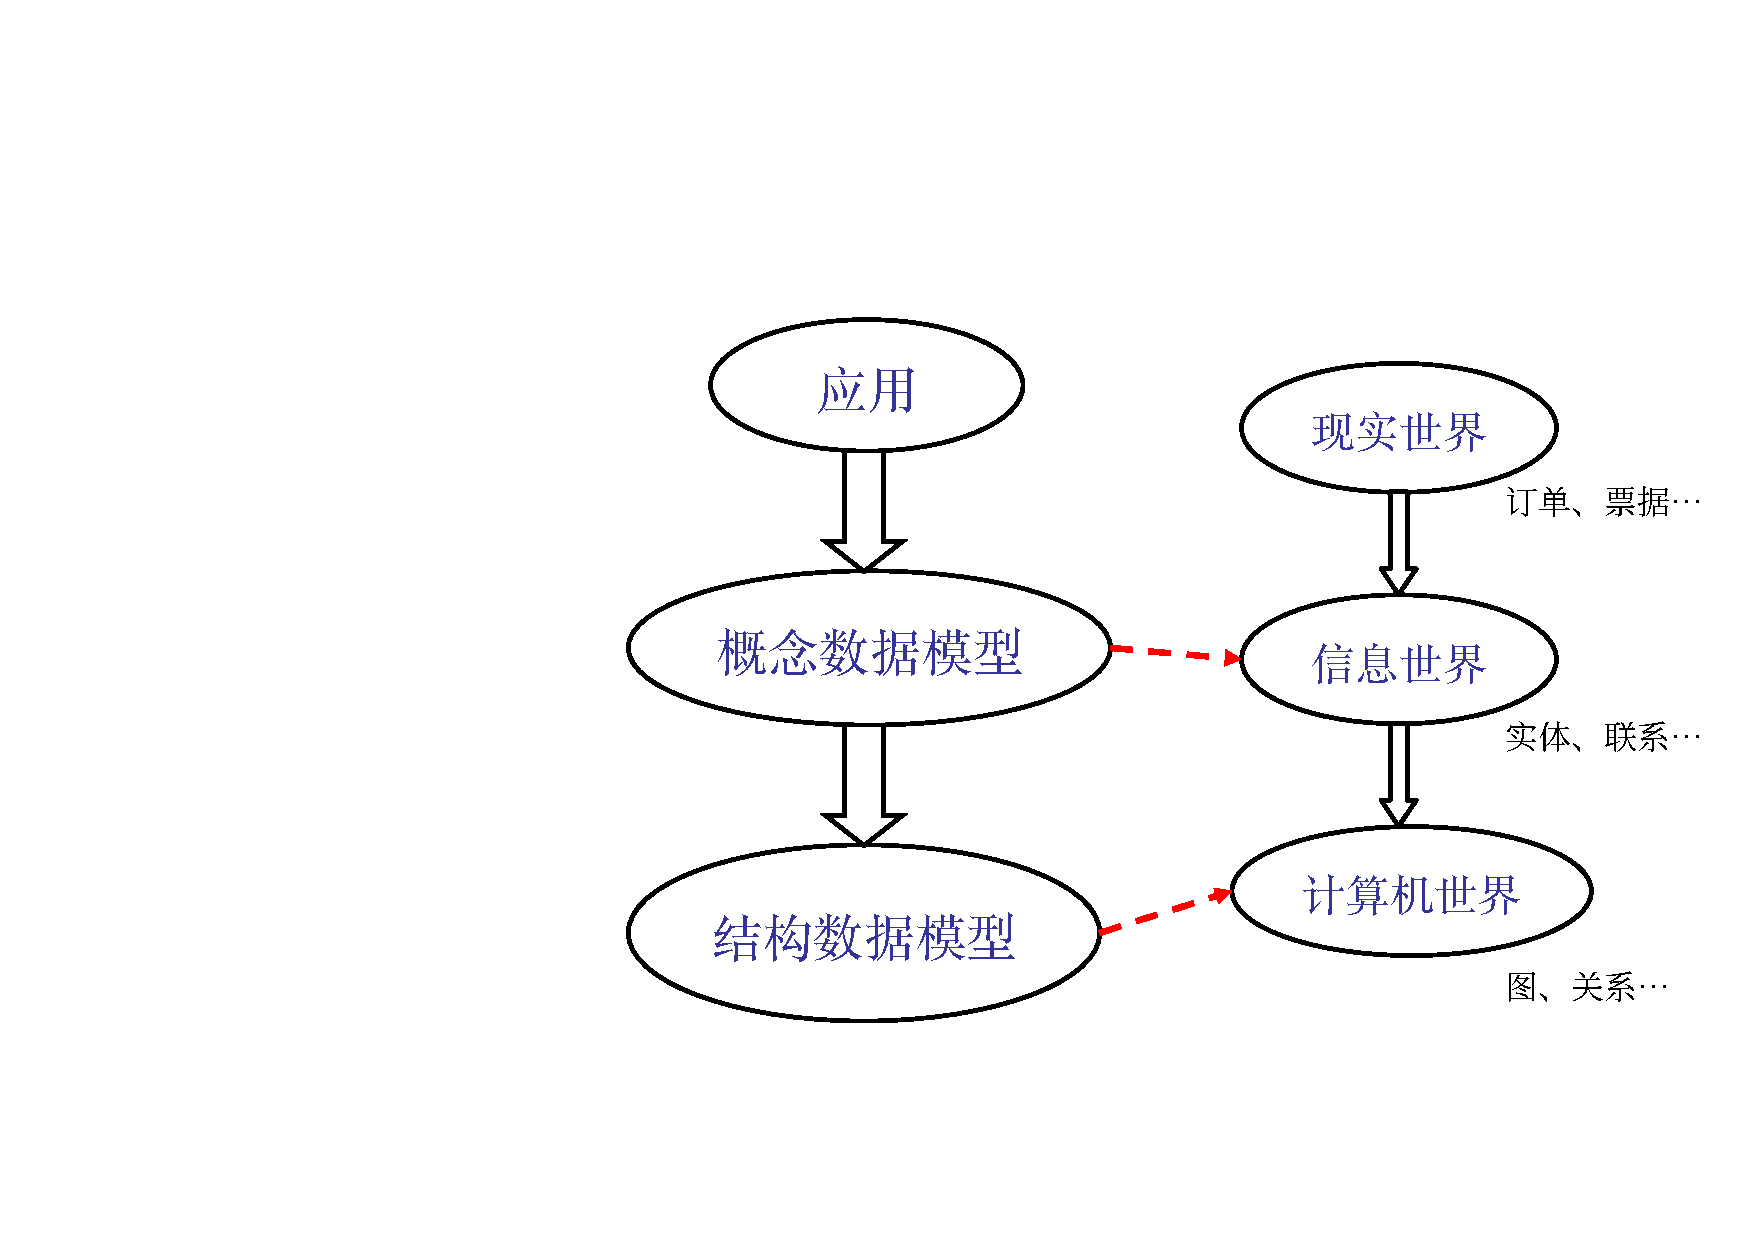
\includegraphics[width=.35\textwidth]{figure/数据模型.pdf}
    \caption{数据模型}
\end{figure}

概念模型: 强调语义表达能力, 给人看
\begin{enumerate}
    \item E-R(实体-联系模型, entity-relationship model).
    \item 基于对象的数据模型(object-based data model)
\end{enumerate}

结构数据模型的概念、种类、特性比较(强调数据结构, 计算机实现, 形式化定义, 给程序看.):
\begin{enumerate}
    \item 层次模型: 使用树状结构表示数据之间的关系, 每个记录只有一个父记录.
    \item 网络模型: 扩展了层次模型, 允许一个记录有多个父记录.
    \item 关系模型: 基于关系理论, 使用表格形式组织数据, 是目前最常用的数据模型.
    \item 面向对象模型: 将数据及其处理方法封装在一起, 支持复杂数据类型.
\end{enumerate}

\begin{figure}[H]
    \centering
    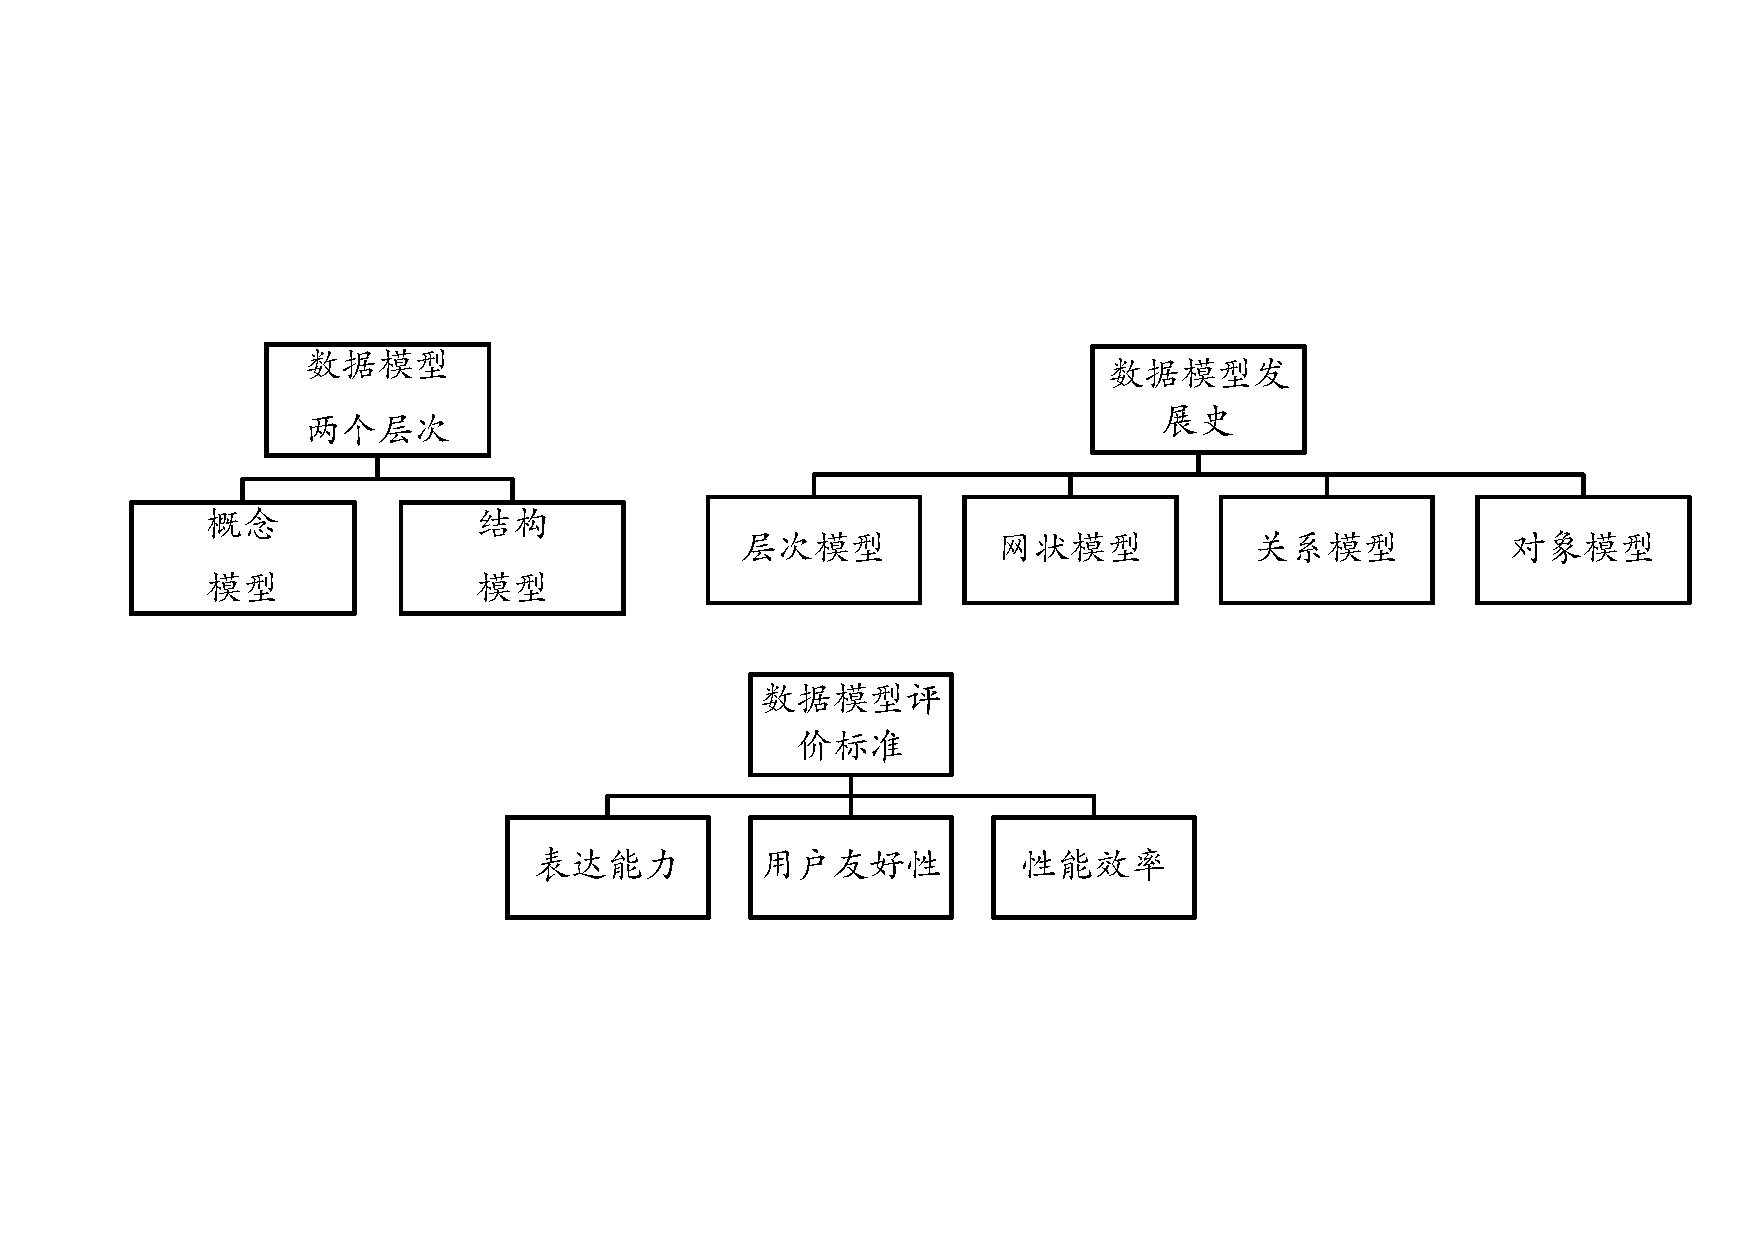
\includegraphics[width=.7\textwidth]{figure/db-5.pdf}
    \caption{数据模式总结}
\end{figure}

\begin{definition}[元数据(metadata)]
元数据是\textcolor{red}{描述数据的数据}.
\end{definition}

所谓\textcolor{red}{数据库模式}, 实际上是一种类型, 而它的值就是数据库当前的一个快照.

数据库系统的架构通常遵循\textcolor{red}{三级模式}和\textcolor{red}{两级映像}的原则.
\begin{enumerate}
    \item 外模式(视图层): 用户看到并与之交互的数据视图.
    \item 模式(逻辑层): 描述数据库中数据的整体逻辑结构.
    \item 内模式(物理层): 定义数据的实际存储方式和访问路径.
    \item 两级映像指的是\textit{外模式/模式映像}和\textit{模式/内模式映像}, 用于保证数据独立性
    \begin{itemize}
        \item 外模式/模式映像: 定义某个外模式和模式之间的对应关系
        \item 模式/内模式映像: 定义数据逻辑结构与存储结构之间的对应关系
    \end{itemize}
\end{enumerate}

\textit{我的理解: 所谓外模式映像就是定义这样一个映射$f$把当前的view映射到某个表上, 内模式映像则是一个映射$g$将某个table映射到存储结构上.}

\begin{figure}[H]
    \centering
    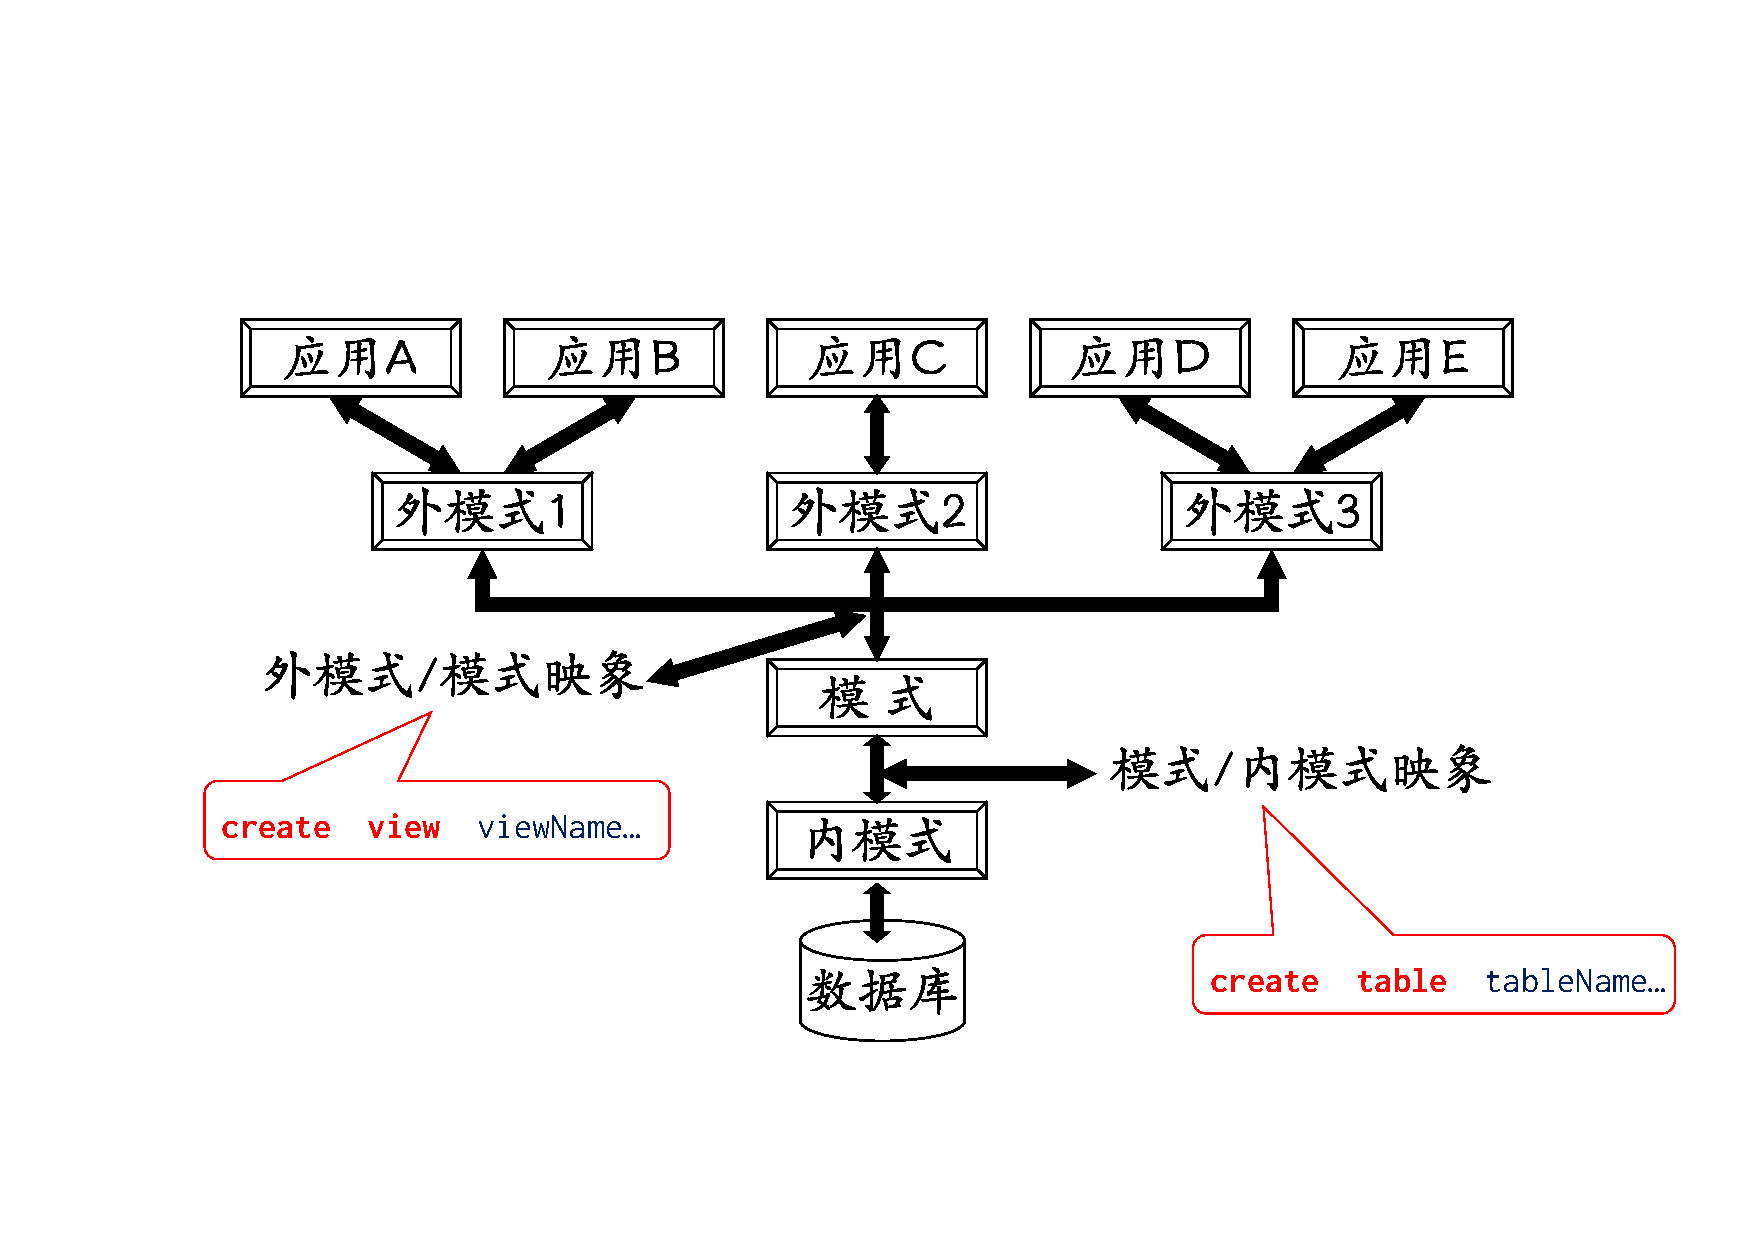
\includegraphics[width=.6\textwidth]{figure/db-6.pdf}
    \caption{数据库的三种模式}
\end{figure}

\begin{remark}
    数据库的逻辑独立性来自于: 外模式/模式映像. 数据库的物理独立性来自于: 模式/内模式映像.
\end{remark}

\begin{figure}[H]
    \centering
    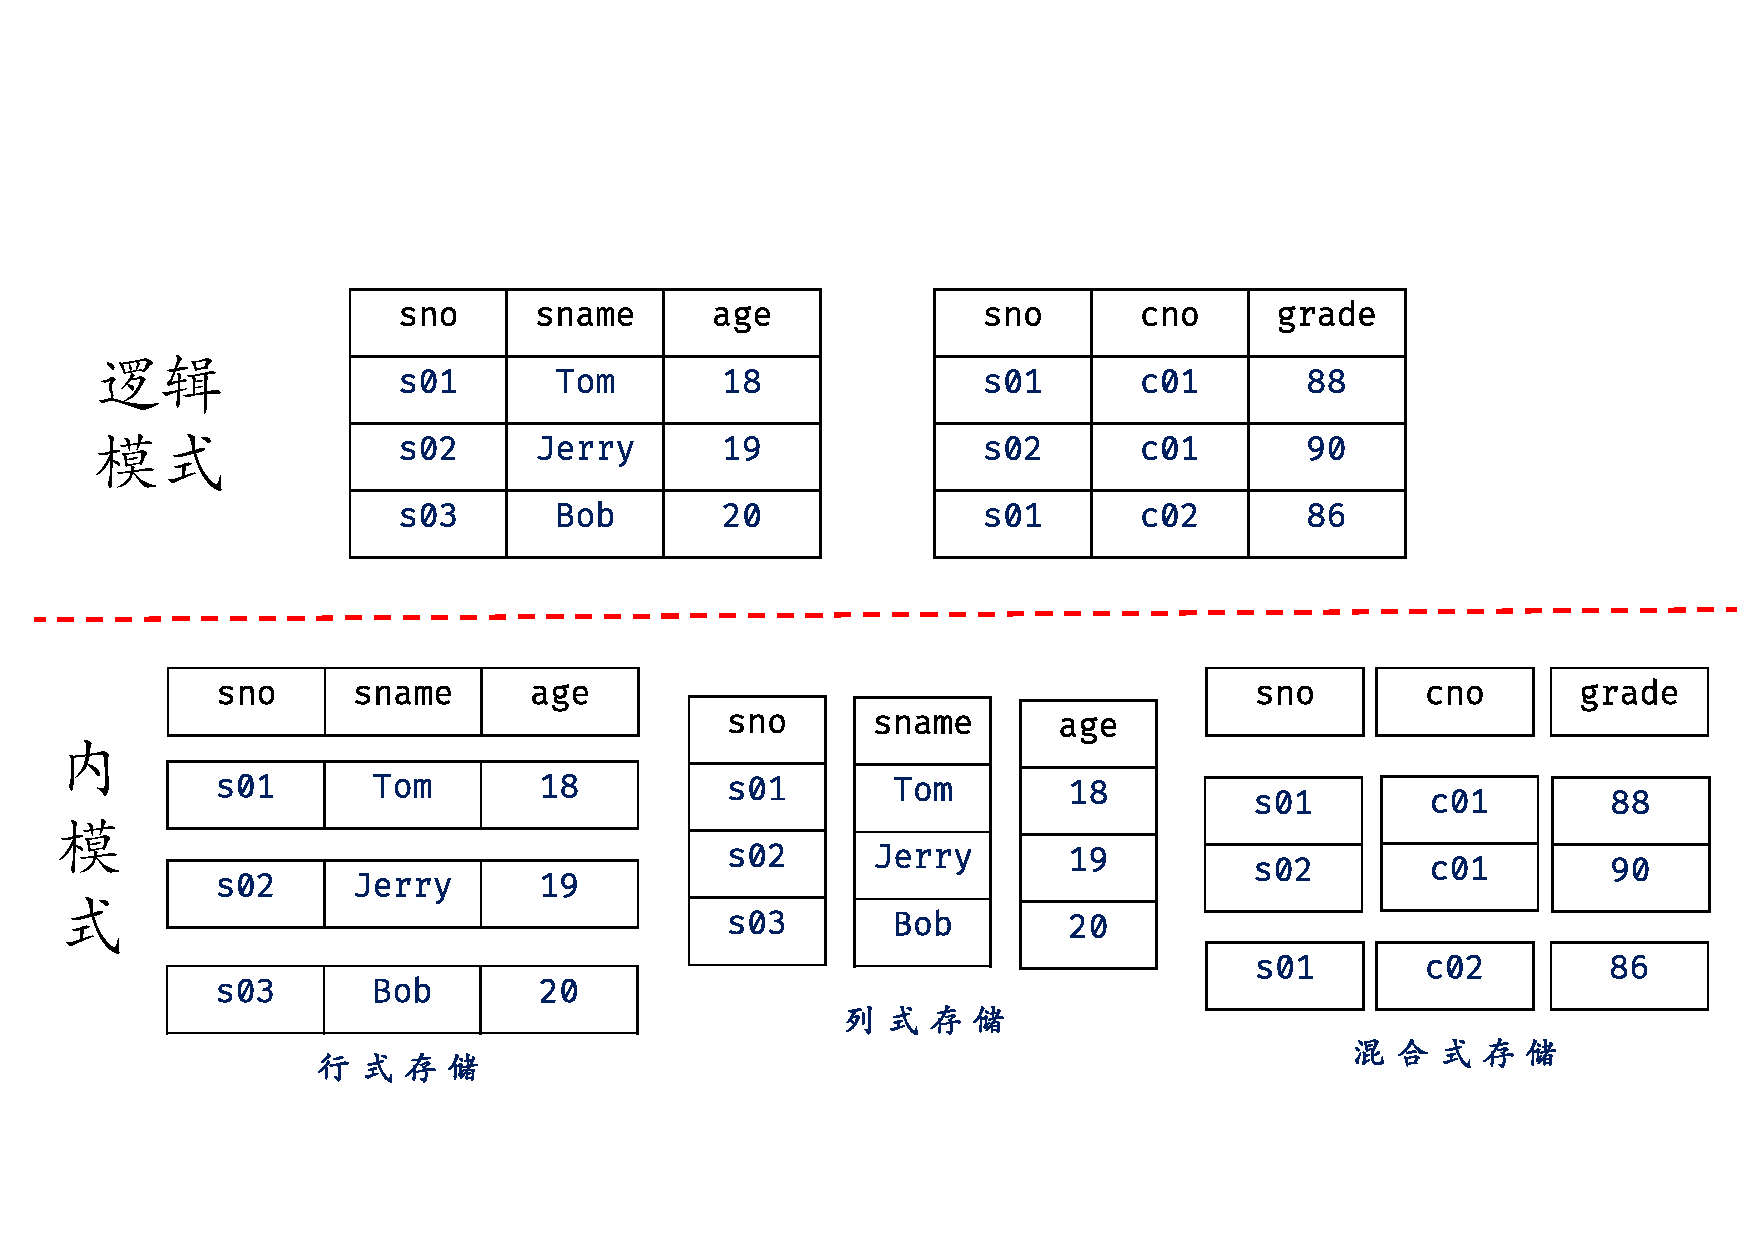
\includegraphics[width=.8\textwidth]{figure/内模式.pdf}
    \caption{数据库内模式的例子}
\end{figure}

\section{数据库系统的构成}

\begin{definition}[数据库]
    数据的集合. 由DBMS统一管理, 多用户共享.
\end{definition}

\begin{definition}[数据库管理系统DBMS]
    系统软件, 对数据库进行统一管理和控制.
\end{definition}

\begin{definition}[数据库系统]
    带有数据库的整个计算机系统, 包括硬件、软件、数据、人员.
\end{definition}

DBMS(数据库管理系统)的功能包括但不限于:
\begin{itemize}
    \item 数据定义: 创建、修改和删除数据库中的对象.
    \item 数据操作: 插入、更新、删除和查询数据库中的数据.
    \item 数据库事务管理: 确保数据库操作的原子性、一致性、隔离性和持久性(ACID属性).
    \item 数据库备份与恢复: 提供机制以防止数据丢失, 并在必要时恢复数据.
\end{itemize}

DBA(数据库管理员)的职责:
\begin{itemize}
    \item 建库方面: 确定模式、外模式、存储结构、存取策略; 负责数据的整理和装入.
    \item 用库方面: 
    \begin{itemize}
        \item 定义完整性约束条件
        \item 规定数据的保密级别、用户权限
        \item 监督和控制数据库的运行情况
        \item 制定后援和恢复策略, 负责故障恢复
    \end{itemize}
    \item 改进方面:
    \begin{itemize}
        \item 监督分析系统的性能(空间利用率, 处理效率)
        \item 数据库重组织, 物理上重组织, 以提高性能
        \item 数据库重构造, 设计上较大改动, 模式和内模式修改
    \end{itemize}
\end{itemize}
 % FINISHED

\chapter{实体-联系模型}

\begin{introduction}[期末考试提纲]
    \item 实体、联系、属性
    \item 超码、候选码、主码
    \item 联系的种类、联系的势
    \item 弱实体、特化、概化、聚集
    \item E-R图概念模型设计应用实例
    \item E-R图和关系模式的相互转换
\end{introduction}

\section{E-R模型基本概念}

E-R模型: Entity-Relation Model.
\begin{itemize}
    \item 世界是由一组称为实体的基本对象和这些对象之间的联系构成的.
    \item \textcolor{red}{实体(Entity)}: \textcolor{red}{客观存在}并\textcolor{red}{可相互区分}的事物叫实体.
    \item 属性(Attribute): 实体具有的某一特性称为属性. 用椭圆表示.
    \item 域(Domain): 属性的取值范围称为域.
    \item 实体型(Entity Type): 实体名+属性名集合. e.g. 学生(学号, 姓名, 年龄, 性别, 系, 年级)
    \item 实体集(Entity Set): 同类型的实体的集合. 用矩形表示.
    \item 联系(Relationship): 实体之间的相互关联. 联系也可以有属性. 用联系表示.
    \item 联系的元(Degree): 参与联系的实体集的个数.
    \begin{itemize}
        \item 学生与学生的班长联系: 一元. 只有一个实体集.
        \item 有时称一元联系为递归联系.
        \item 联系是发生在实体集之间的还是实体型之间的? \textbf{实体集.}
    \end{itemize}
    \item 实体集属性中作为主码的一部分的属性用\underline{下划线}来标明.
\end{itemize}

\begin{figure}[H]
    \centering
    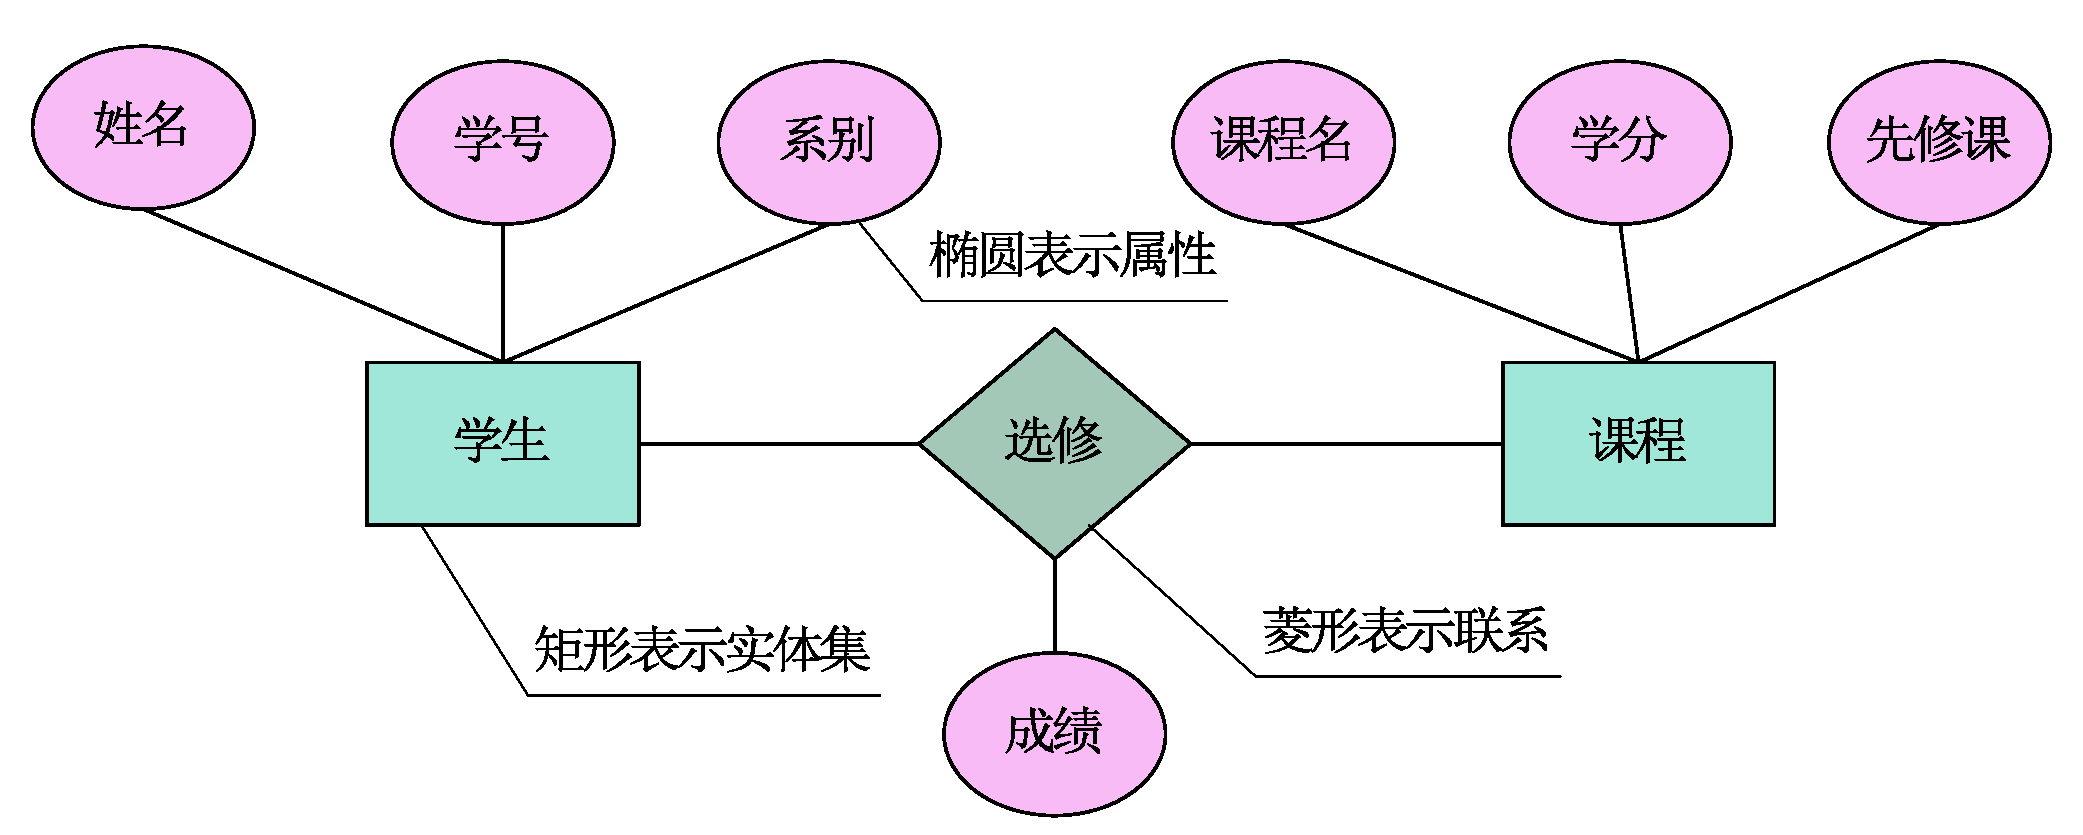
\includegraphics[width=.8\textwidth]{figure/db-8.pdf}
    \caption{E-R图}
\end{figure}

表达一元联系:
\begin{figure}[H]
    \centering
    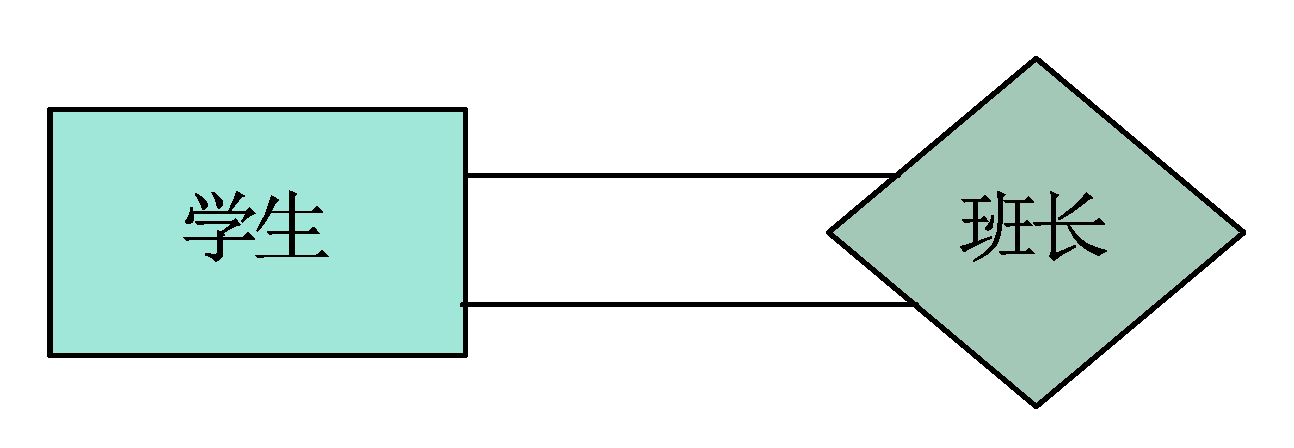
\includegraphics[width=.3\textwidth]{figure/db-9.pdf}
    \caption{一元联系}
\end{figure}

\section{实体的码(Key)}

\begin{definition}[超码(Superkey)]
    能\textcolor{red}{唯一标识实体}的属性或者属性组. 超码的任意超集也是超码.
\end{definition}

\begin{definition}[候选码(candidate key)]
    其任意真子集都不能成为超码的最小超码.
\end{definition}

\begin{definition}[主码(primary key)]
    选定的候选码作为实体的标识码.
\end{definition}

\begin{definition}[替代码]
    除去主码的其他候选码. (可以替代主码的候选码)
\end{definition}

\begin{definition}[代理码]
    人为添加的属性作为主码. e.g. ssn(单纯的随机码)
\end{definition}

\begin{definition}[自然码]
    e.g. 不重名的情况下, 姓名可以作为候选码. “真正的”候选码.
\end{definition}

\begin{definition}[智能码]
    经过编码的标识符. e.g. 学号, 电话号码, 身份证
\end{definition}

\section{属性}

属性包括: 复合、多值、派生、NULL.

\begin{definition}[简单属性]
     不可再分的属性. e.g. 学号, 姓名
\end{definition}

\begin{definition}[复合属性(Composite)]
    可以划分为更小的属性. e.g. 电话号码=区号+号码, 地址=省+市+区+街道+门牌号, 日期=年+月+日.
\end{definition}

\begin{definition}[单值属性]
    每一个特定的实体在该属性上的取值唯一.
\end{definition}

\begin{definition}[多值属性]
    多于一个的取值(取值是一个集合. 必须展开.)
\end{definition}

\begin{definition}[派生属性(Derived)]
    可以从其他属性或者实体派生出来的值. e.g., 绩点可以通过成绩计算出来.
\end{definition}

\begin{definition}[NULL 属性]
    值存在但是目前没有获得其信息. / 当实体在某个属性上没有值时设为 NULL.

    \textcolor{red}{实体完整性: 主码取值不能为 NULL.}
\end{definition}

\begin{figure}[H]
    \centering
    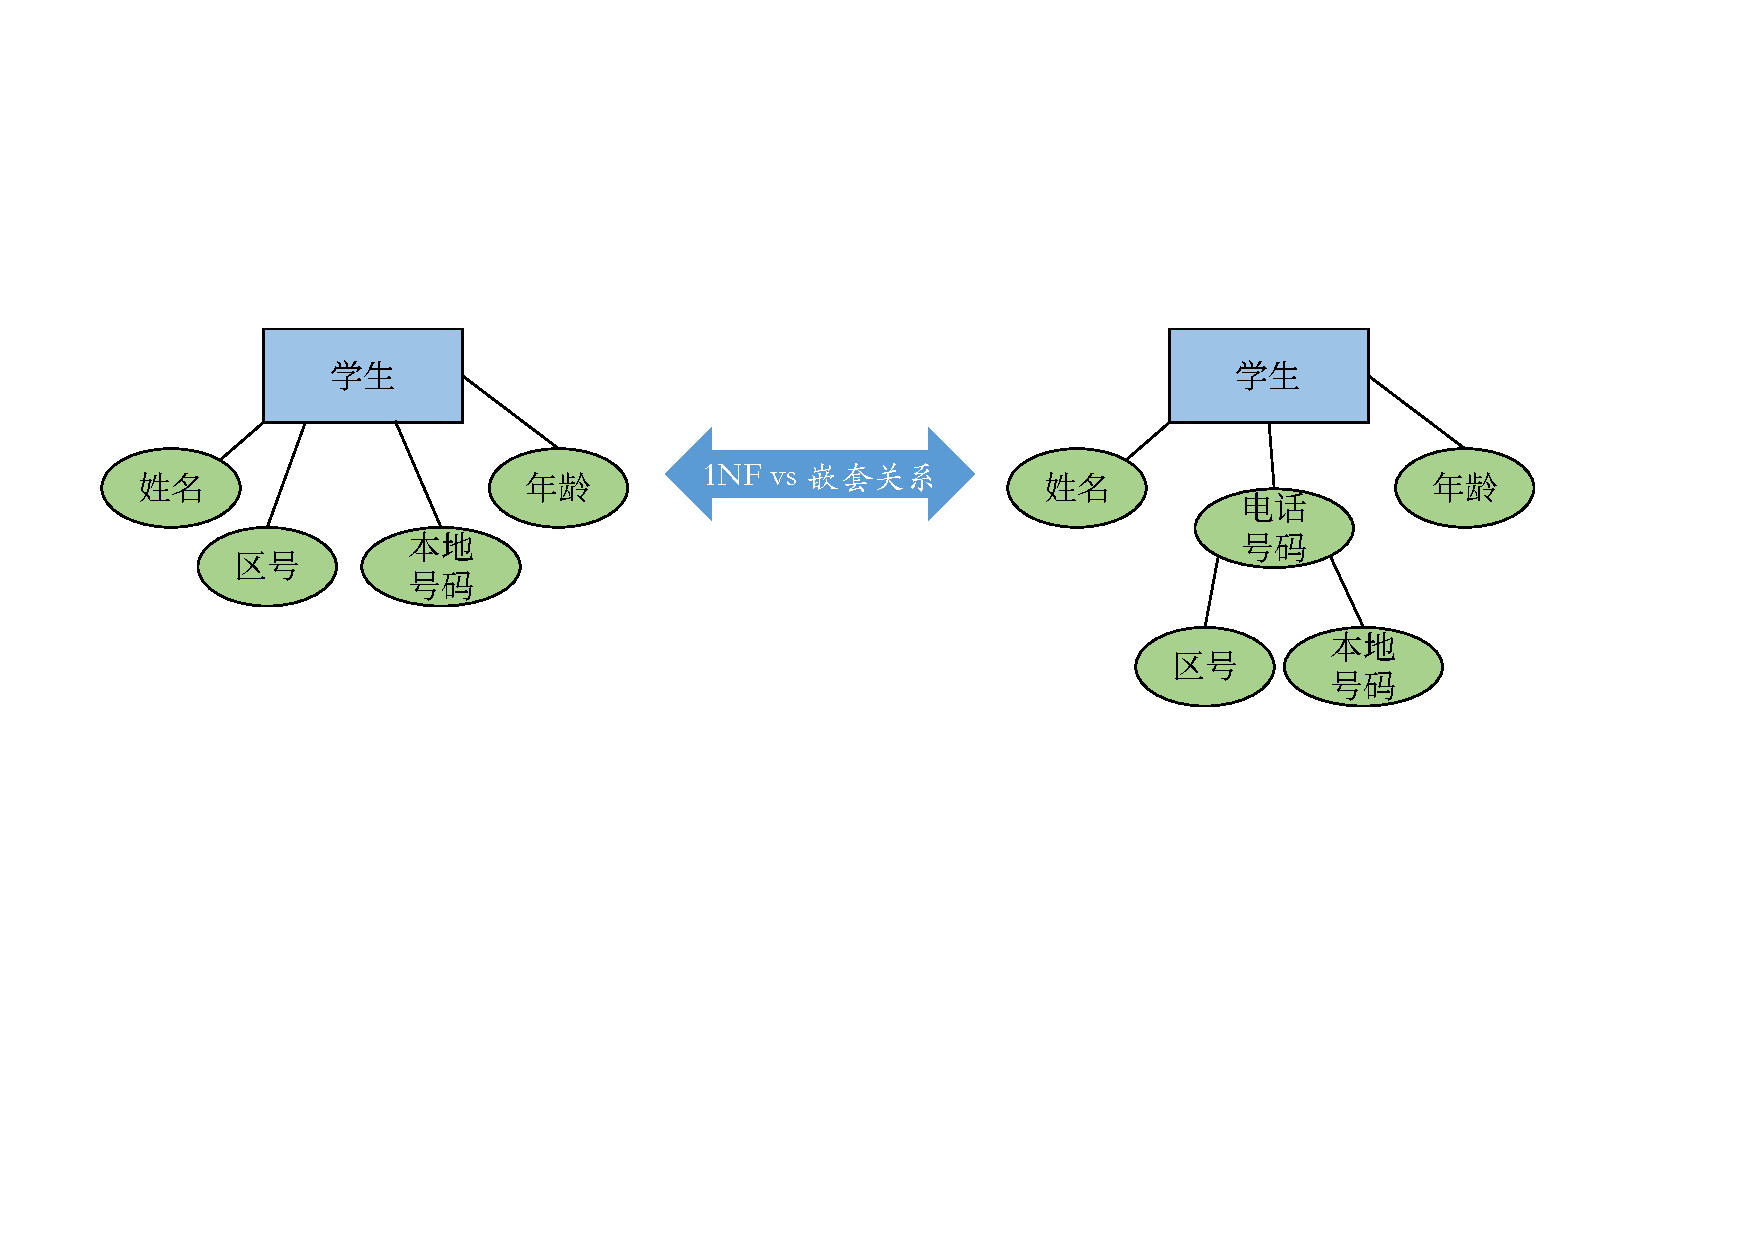
\includegraphics[width=.8\textwidth]{figure/多值.pdf}
    \caption{简单属性 vs 复合属性}
\end{figure}

\begin{figure}[H]
    \centering
    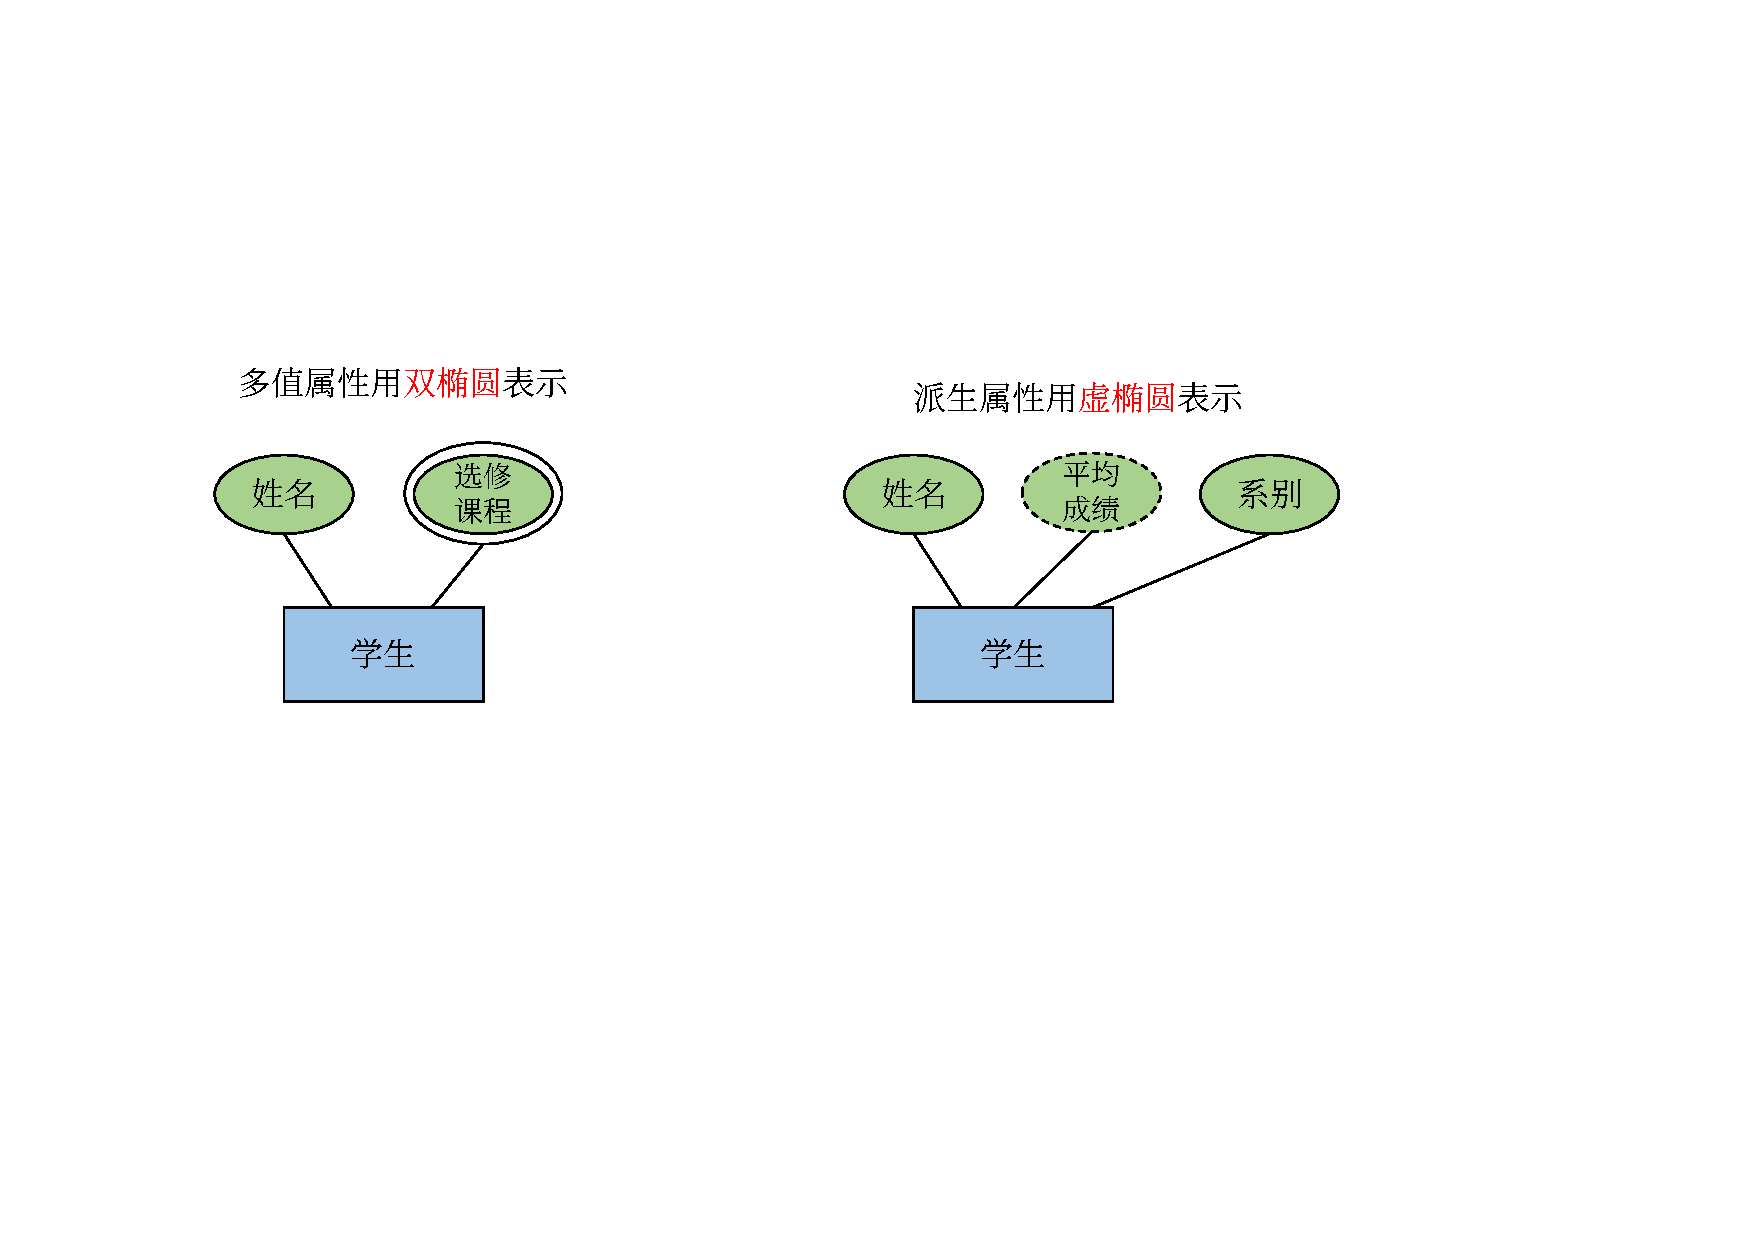
\includegraphics[width=.8\textwidth]{figure/多值属性和派生属性.pdf}
    \caption{多值属性和派生属性的表示}
\end{figure}

\section{联系}

注: 在多方实体和联系之间的线段上标注字母; 在单方实体和联系之间的线段上标注数字1.
\begin{figure}[H]
    \centering
    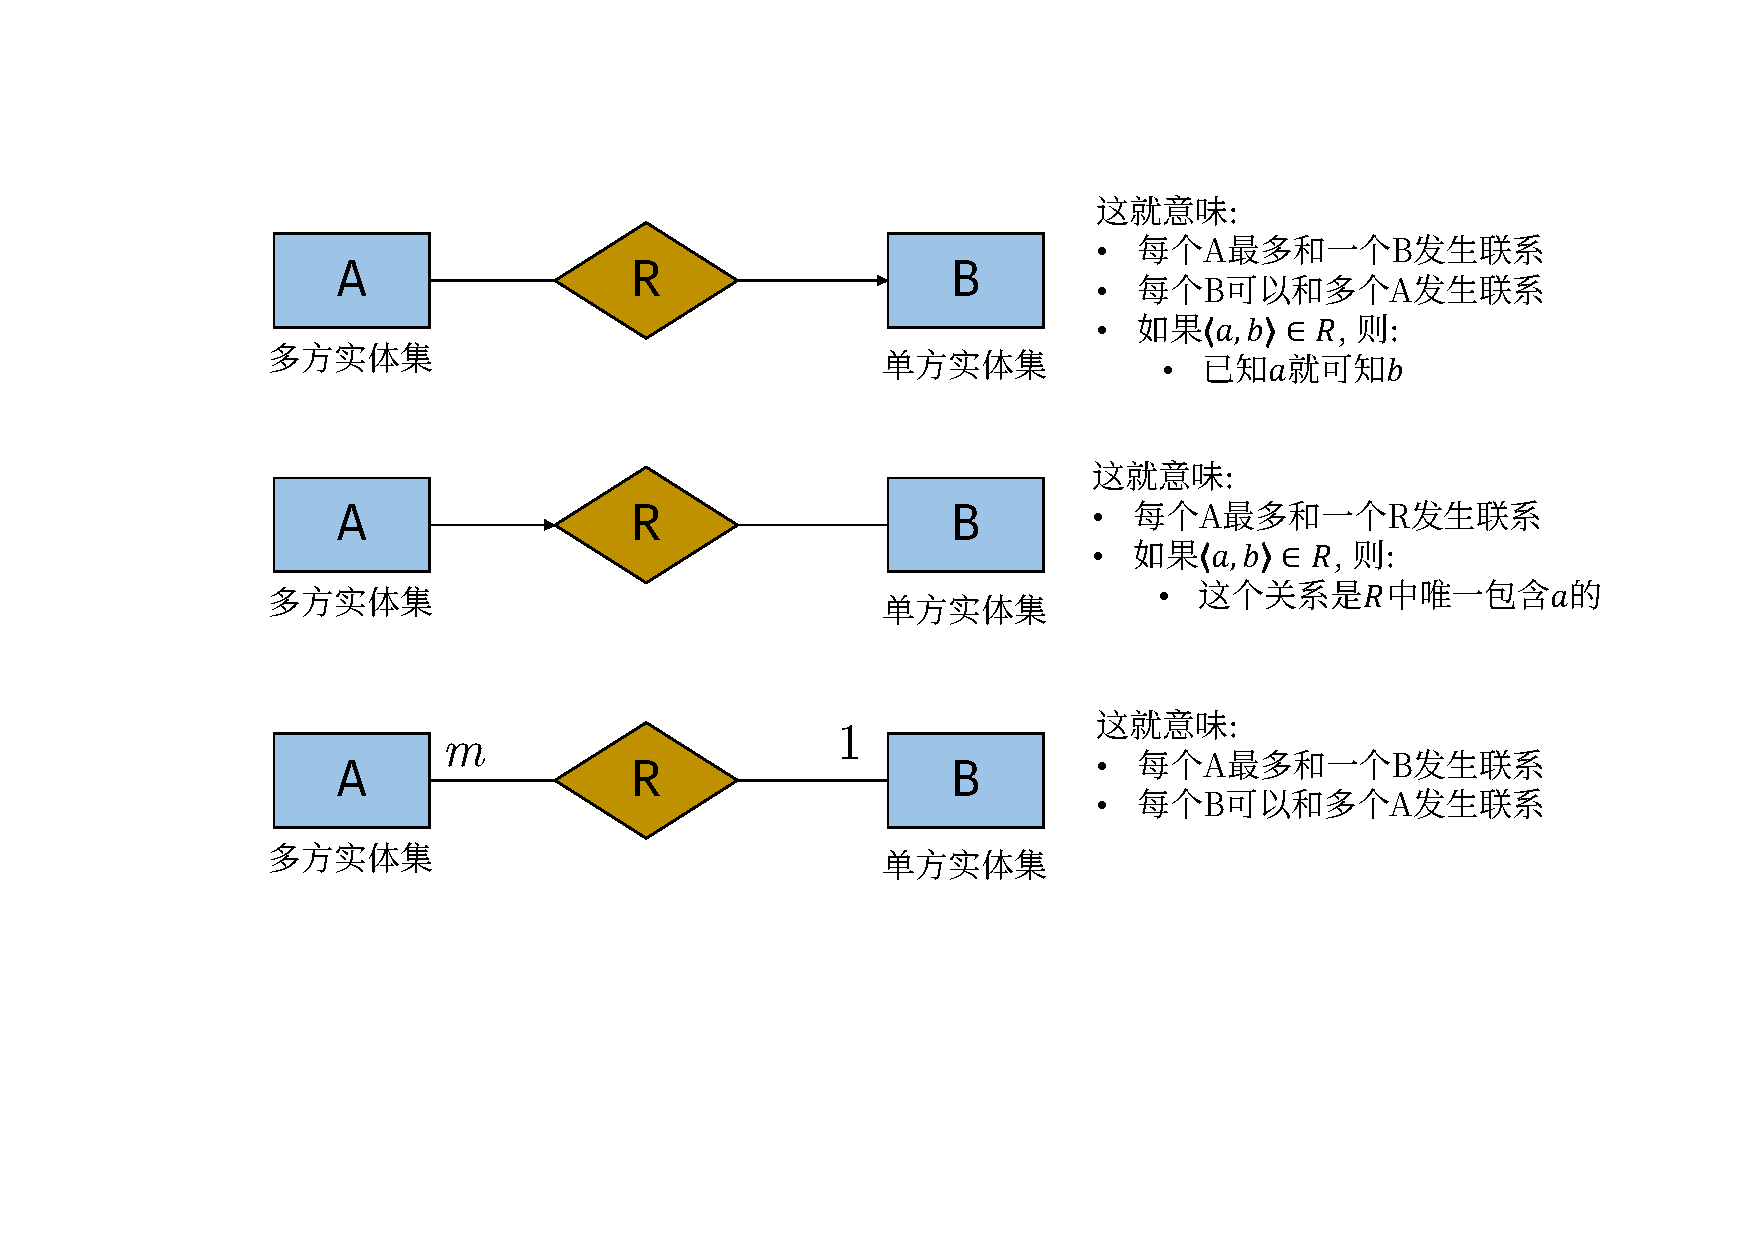
\includegraphics[width=.7\textwidth]{figure/联系.pdf}
    \caption{联系种类在E-R图中的表示}
\end{figure}

\begin{definition}[联系的数量]
    实体之间的\textcolor{red}{联系的数量}, 即一个实体通过一个联系集能与另
    一实体集相关联的实体的数目.
    \begin{itemize}
        \item 一对一的 (1:1)
        \item 一对多的 (1:$m$)
        \item 多对多的 ($m:n$)
    \end{itemize}
\end{definition}

用箭头或线段来表示联系的种类, \textcolor{red}{箭头指向单方实体集}.


二元联系的种类:
\begin{definition}[一对一联系]
    两个实体集$E_1,E_2$之间的一对一联系:
    \begin{itemize}
        \item $E_1$中的一个实体与$E_2$中至多一个实体相联系;
        \item $E_2$中的一个实体与$E_1$中至多一个实体相联系.
    \end{itemize}
    \textcolor{red}{一对一不是一一对应!!!}
\end{definition}

\begin{figure}[H]
    \centering
    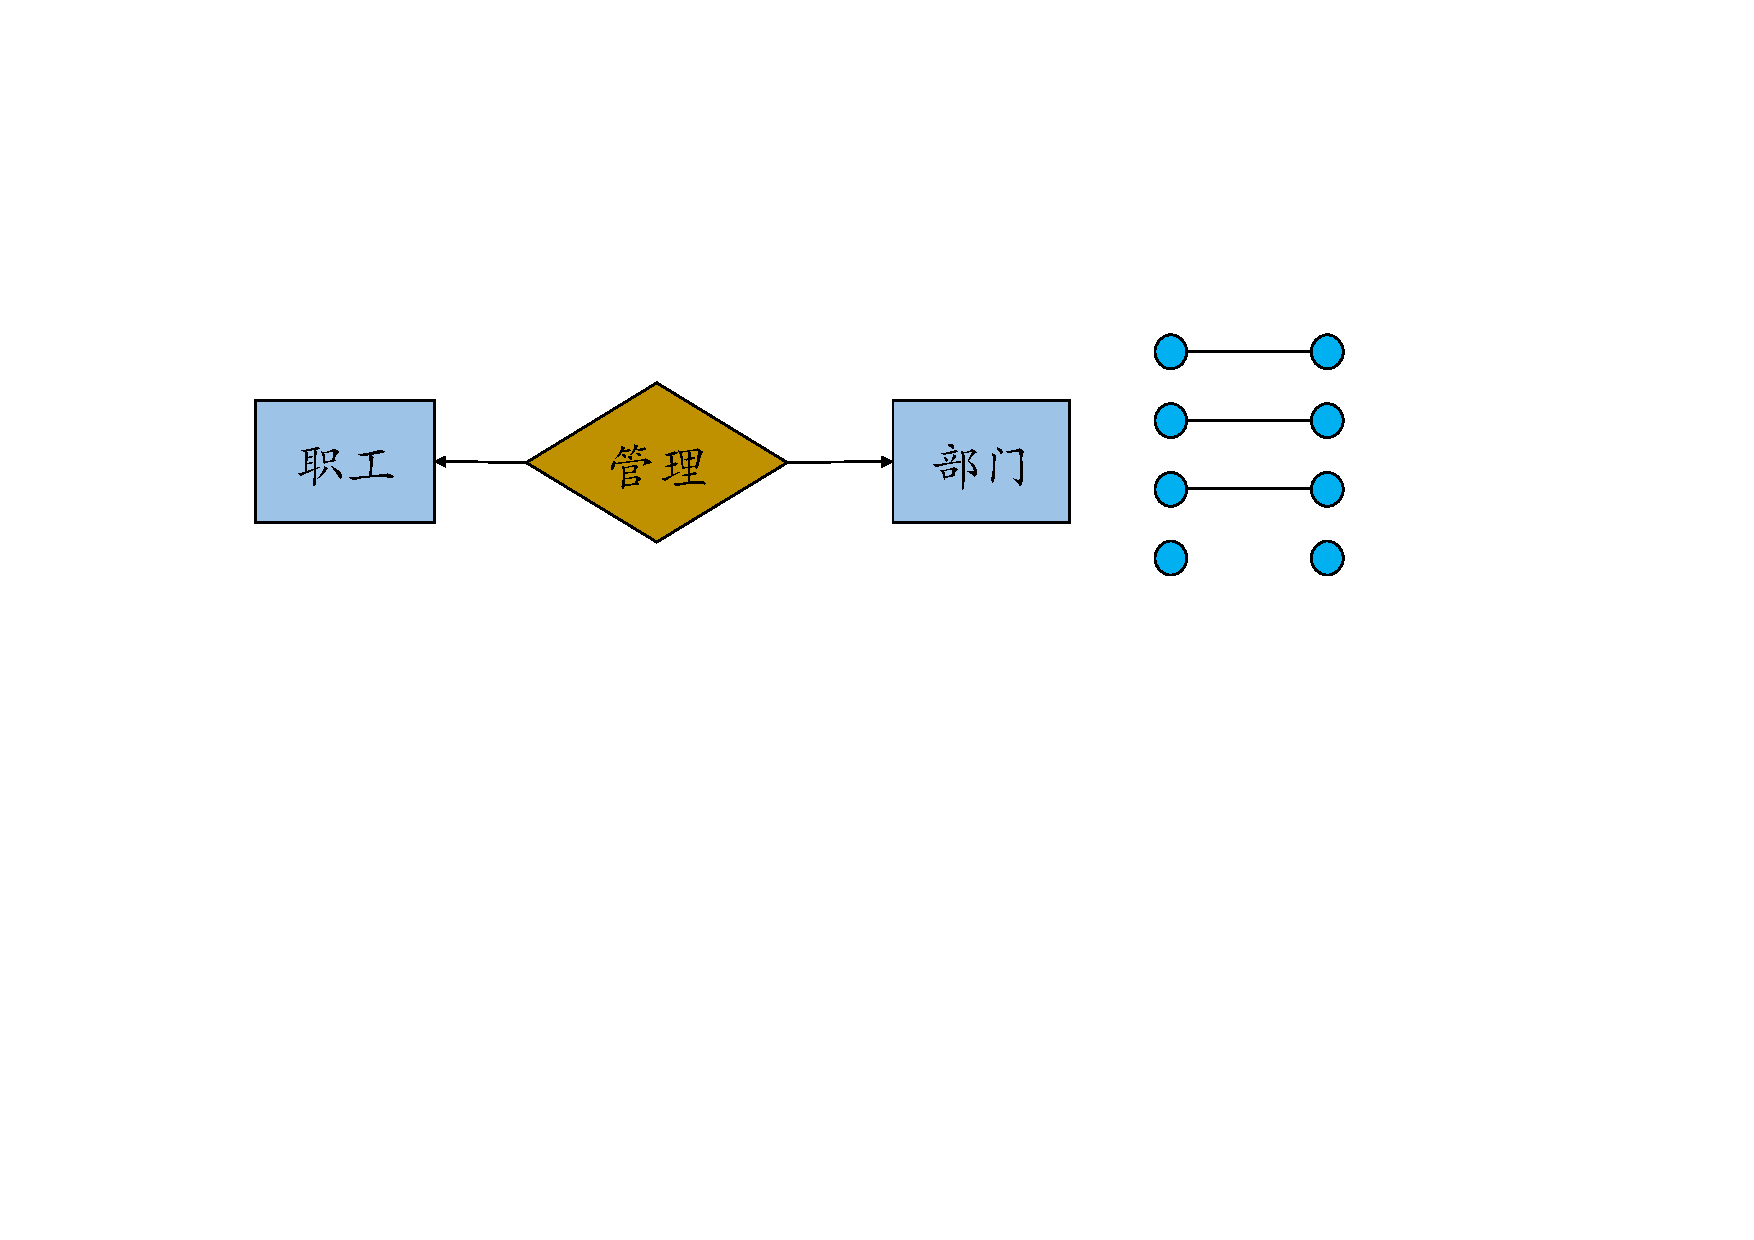
\includegraphics[width=.6\textwidth]{figure/一对一.pdf}
    \caption{一对一联系}
\end{figure}


\begin{definition}[一对多联系]
    两个实体集$E_1,E_2$之间的一对多联系:
    \begin{itemize}
        \item $E_1$中的一个实体与$E_2$中$n(n\geq 0)$个实体相联系;
        \item $E_2$中的一个实体与$E_1$中至多一个实体相联系.
    \end{itemize}
\end{definition}

\begin{figure}[H]
    \centering
    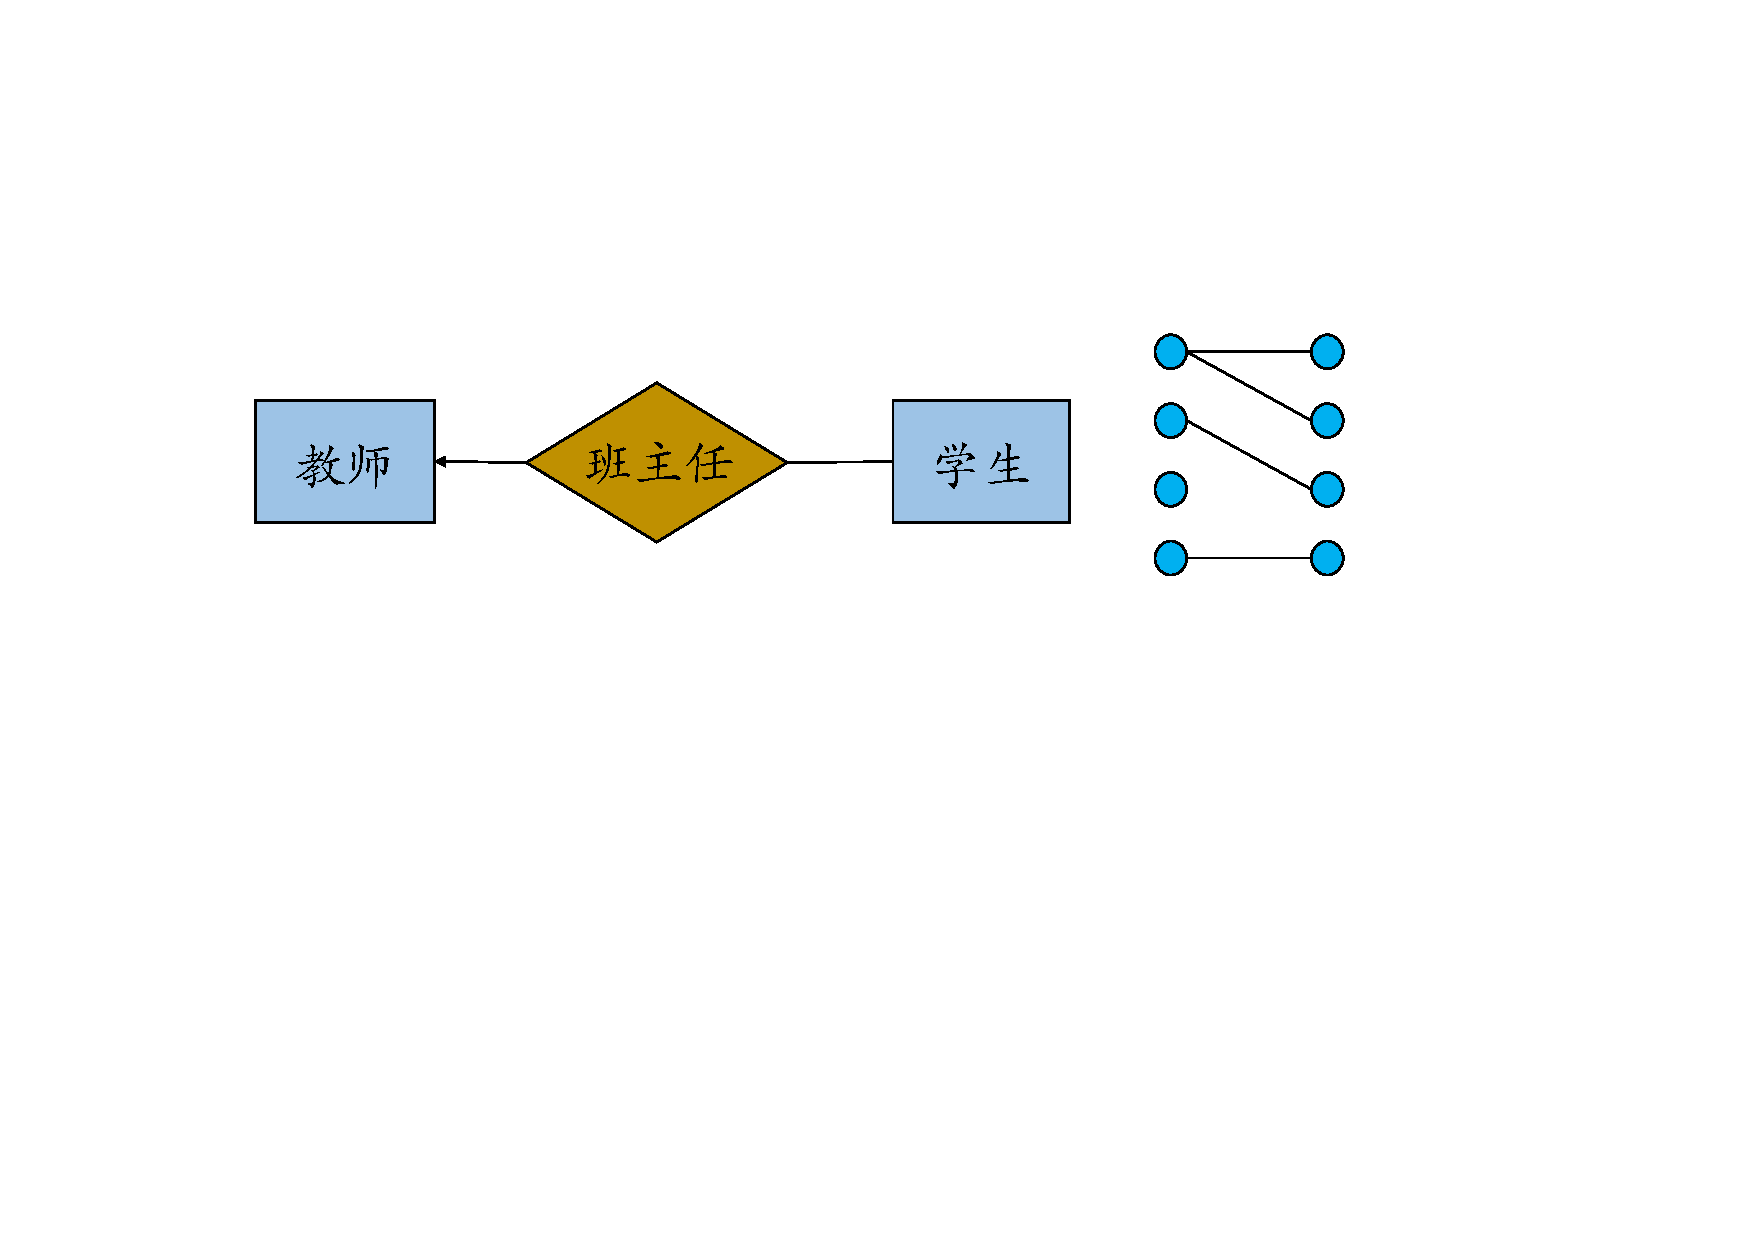
\includegraphics[width=.6\textwidth]{figure/一对多.pdf}
    \caption{一对多联系}
\end{figure}

\begin{definition}[多对多联系]
    两个实体集$E_1,E_2$之间的多对多联系:
    \begin{itemize}
        \item $E_1$中的一个实体与$E_2$中$n(n\geq 0)$个实体相联系;
        \item $E_2$中的一个实体与$E_1$中$m(m\geq 0)$个实体相联系.
    \end{itemize}
\end{definition}

\begin{figure}[H]
    \centering
    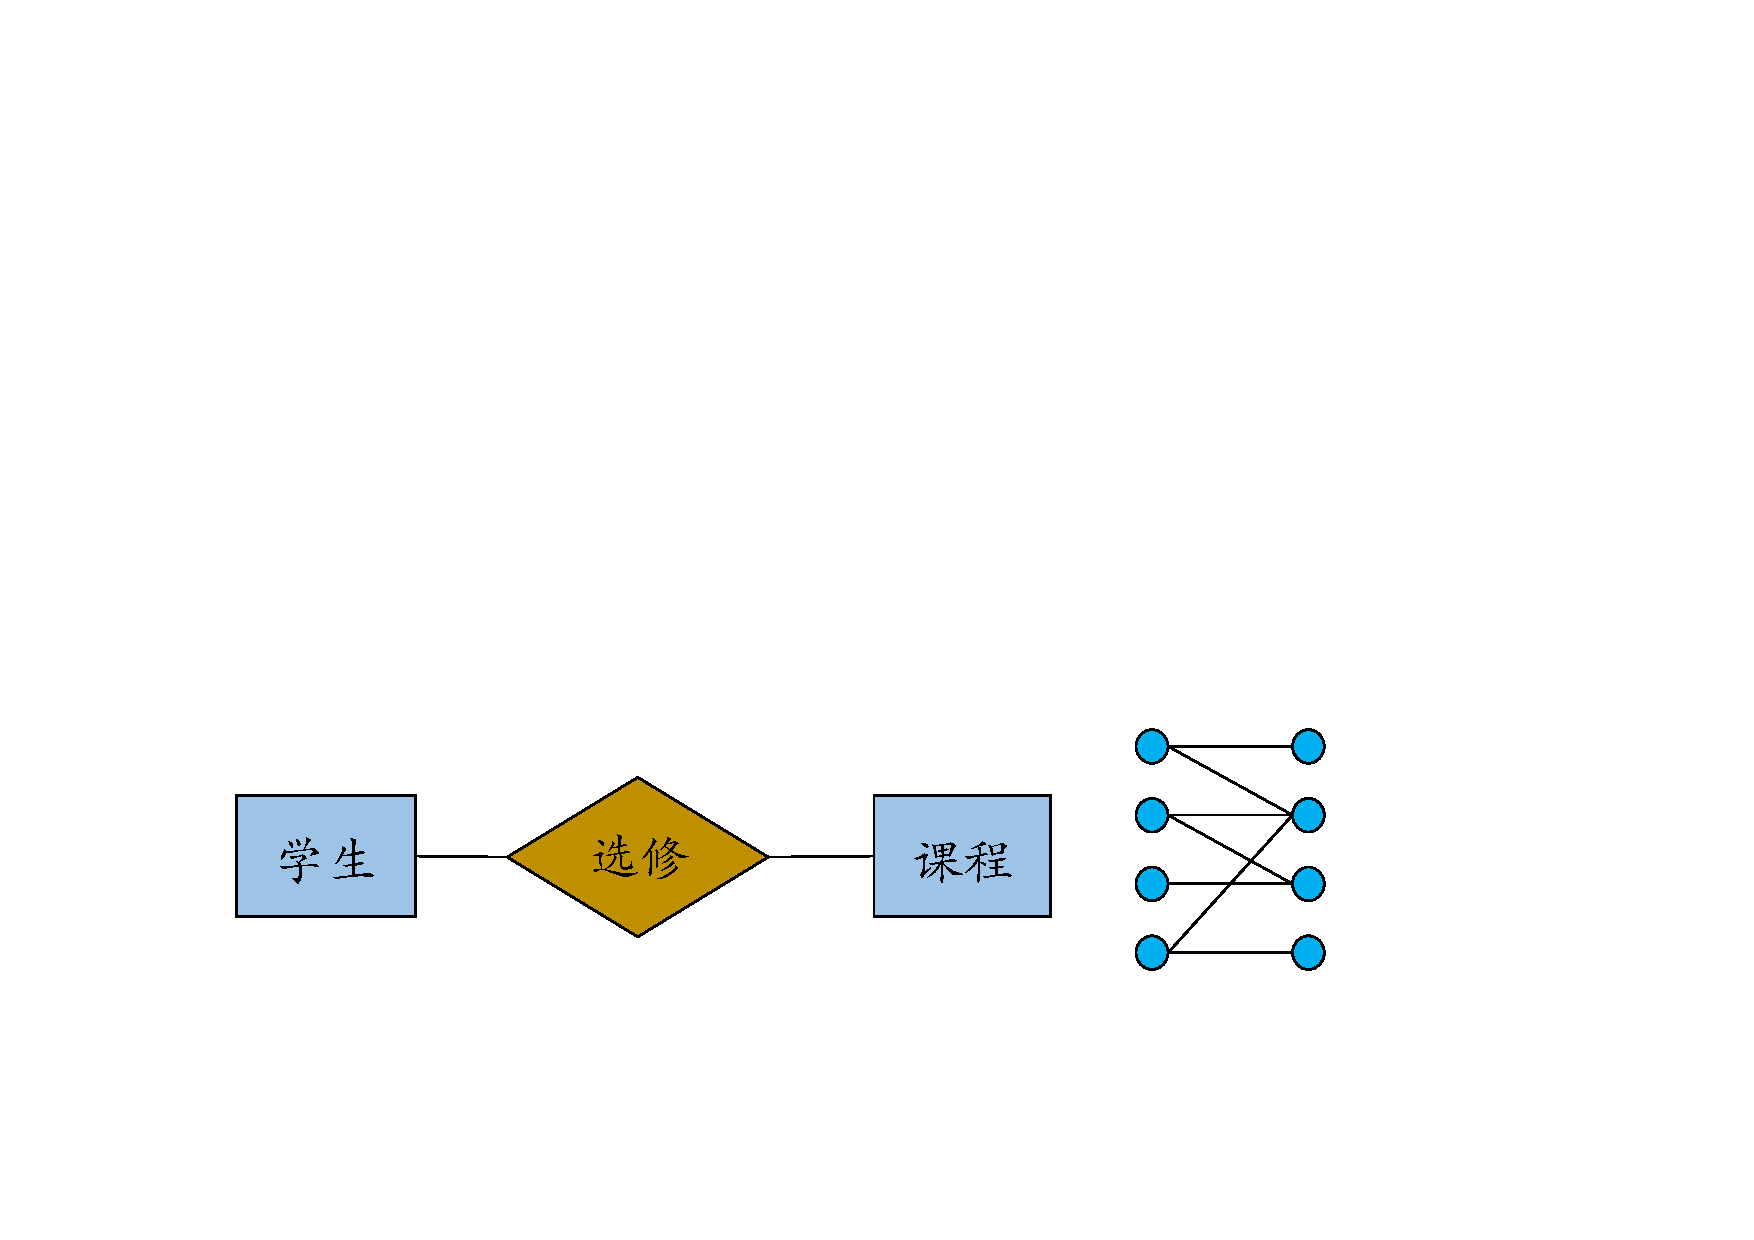
\includegraphics[width=.6\textwidth]{figure/多对多.pdf}
    \caption{多对多联系}
\end{figure}

\textbf{一个实体集内的递归联系:}

\begin{figure}[H]
    \centering
    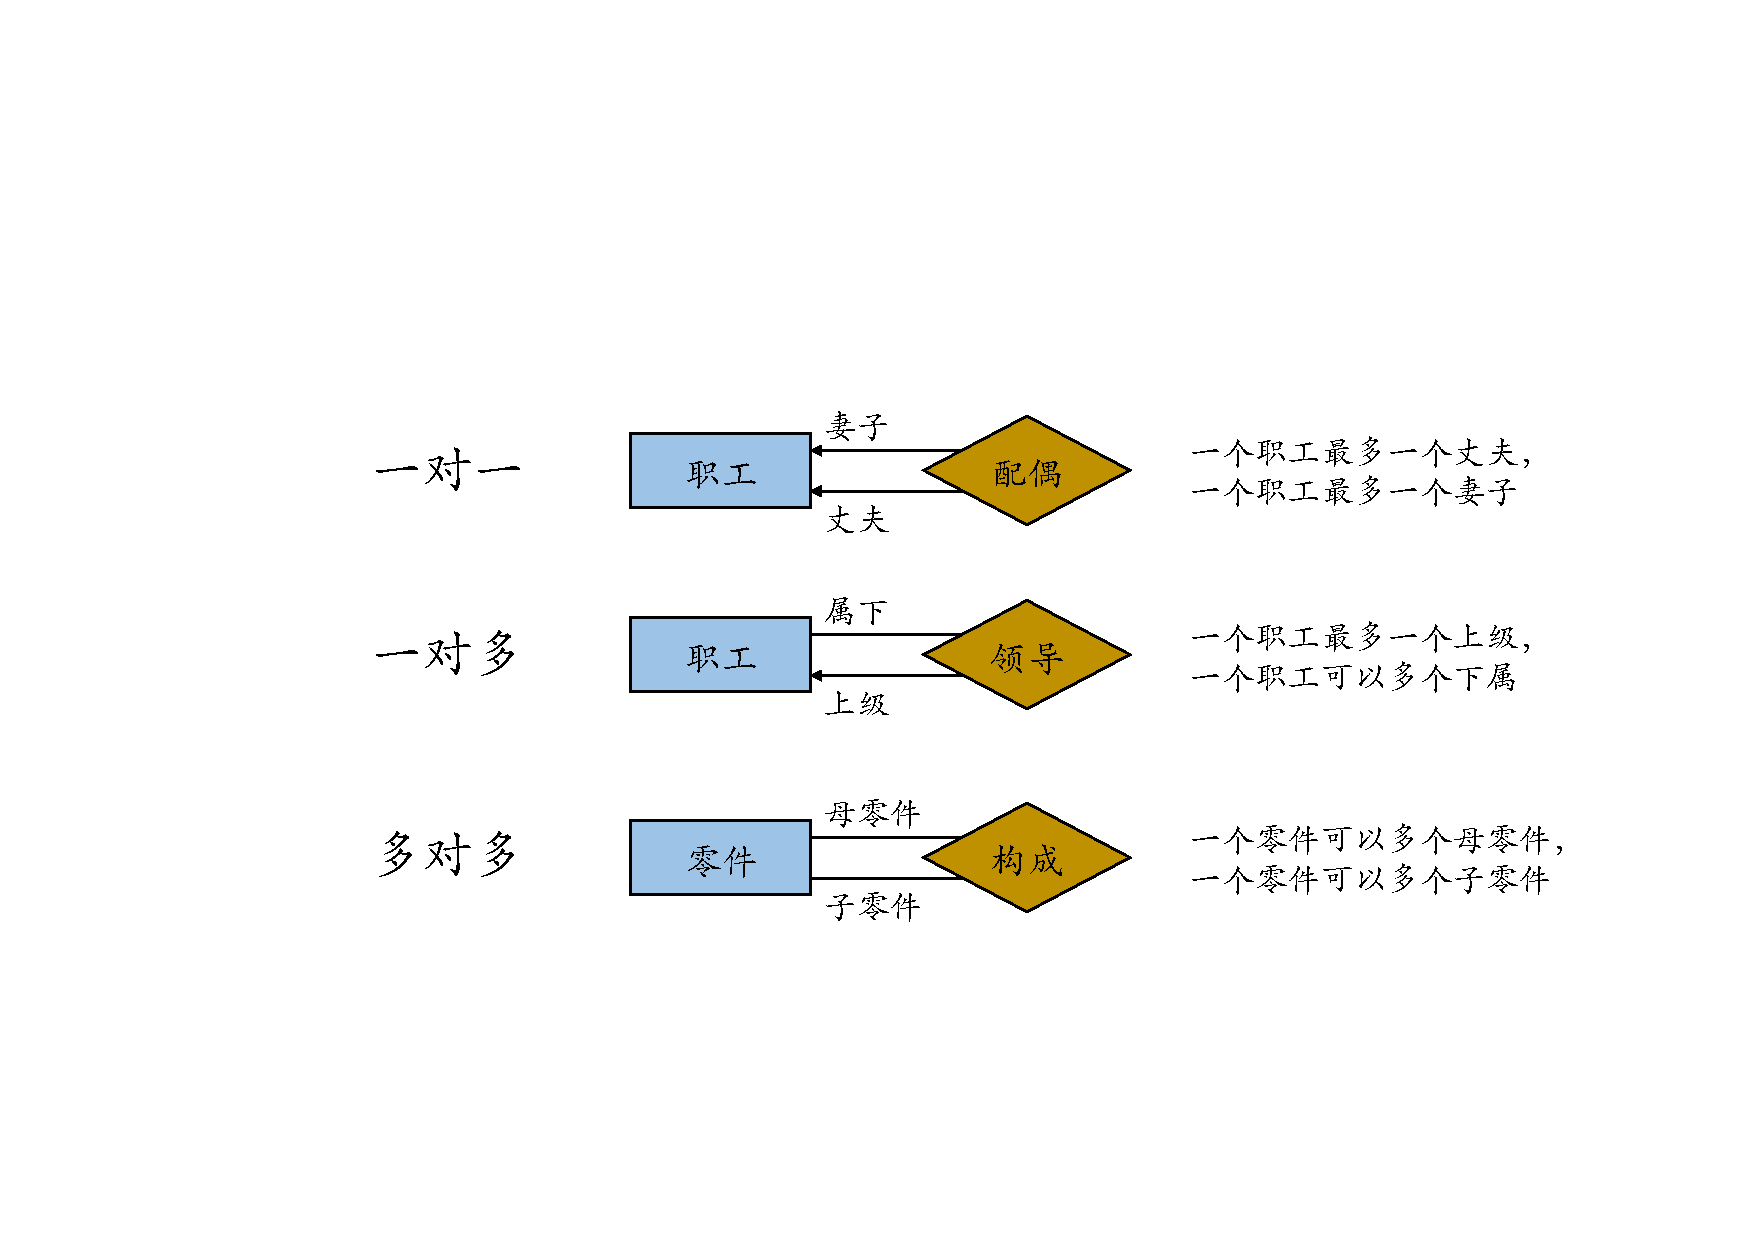
\includegraphics[width=.7\textwidth]{figure/递归联系.pdf}
    \caption{一个实体集内的递归联系}
    \label{n-ary-link}
\end{figure}

\begin{definition}[多元联系]
    当一个联系涉及三个或更多实体集时, 我们称之为多元联系.
\end{definition}

\begin{figure}[H]
    \centering
    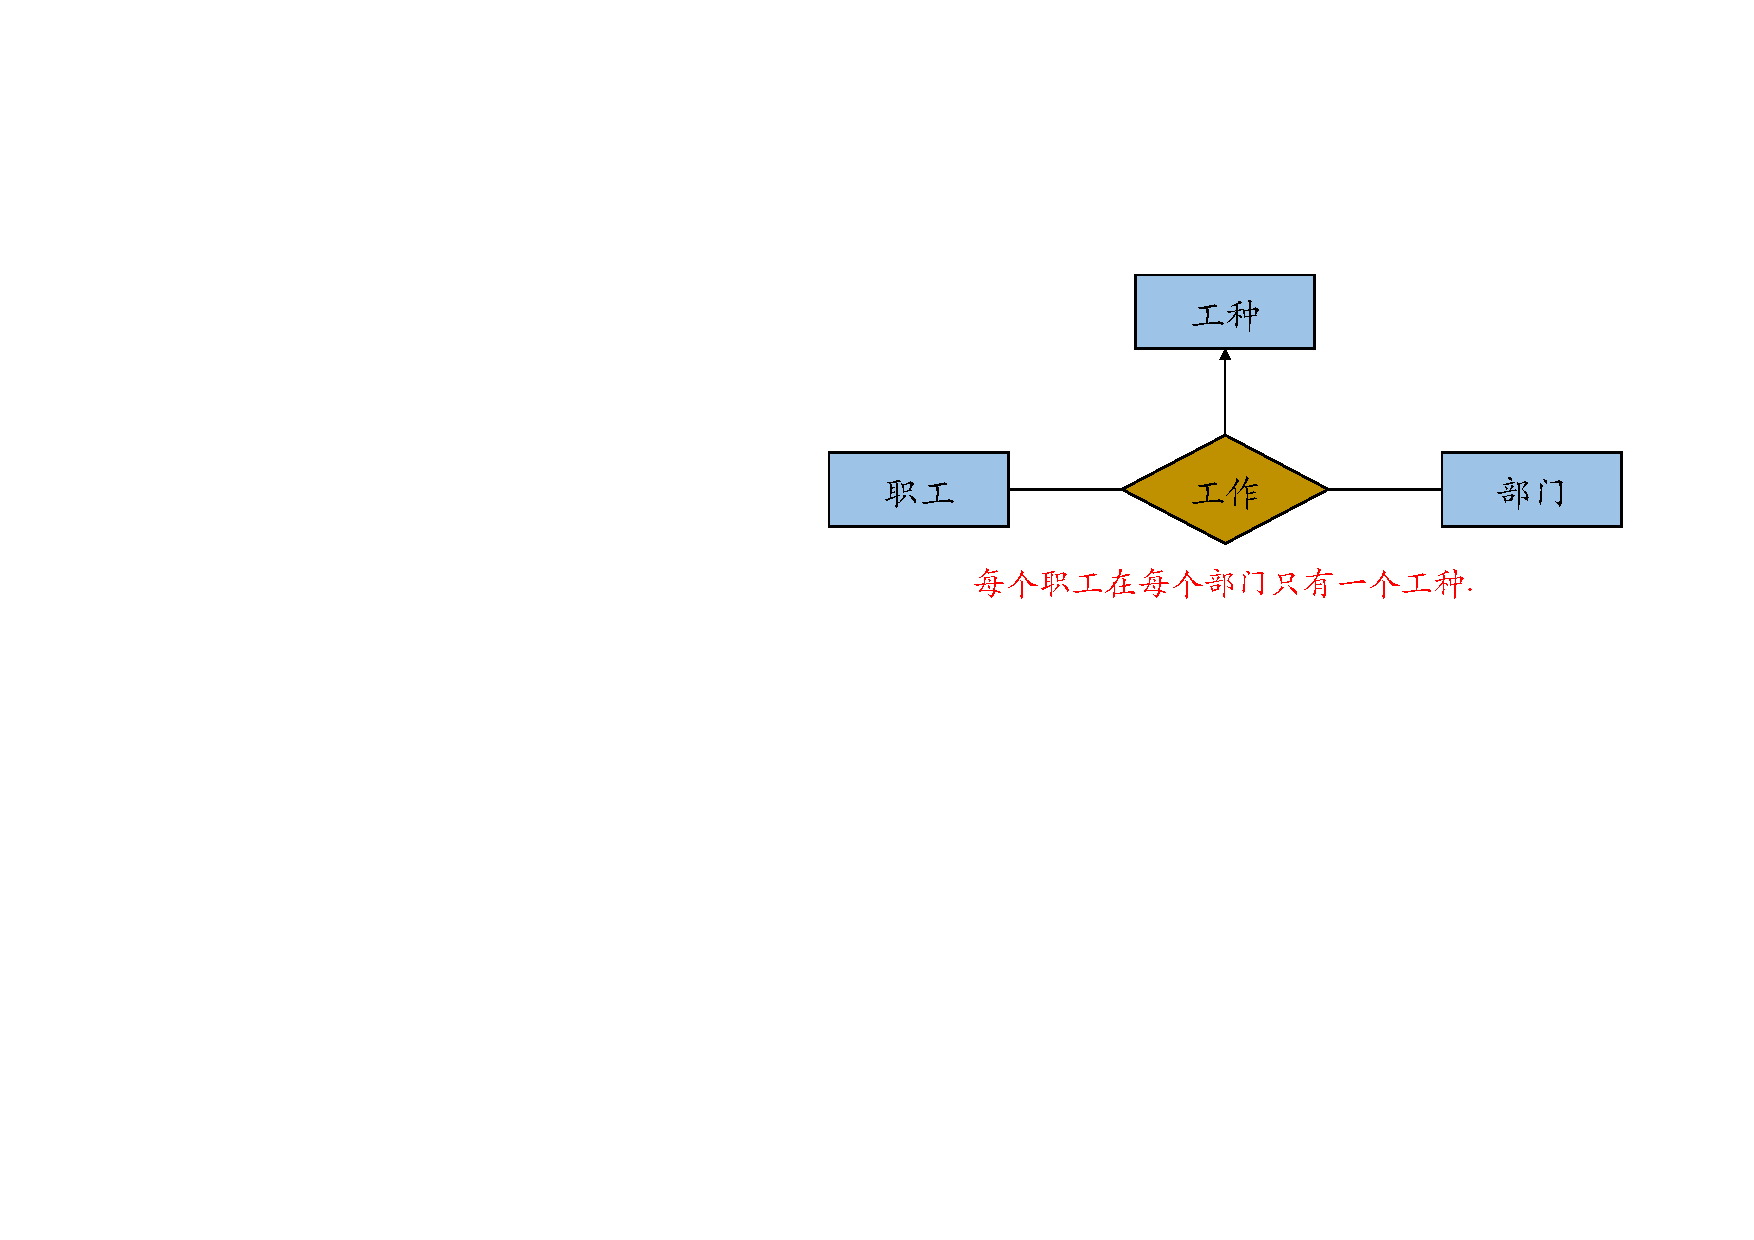
\includegraphics[width=.5\textwidth]{figure/多元联系.pdf}
    \caption{多元联系}
\end{figure}

\begin{definition}[联系的势]
    势表达了一个实体出现在联系中的次数.
\end{definition}

\begin{figure}[H]
    \centering
    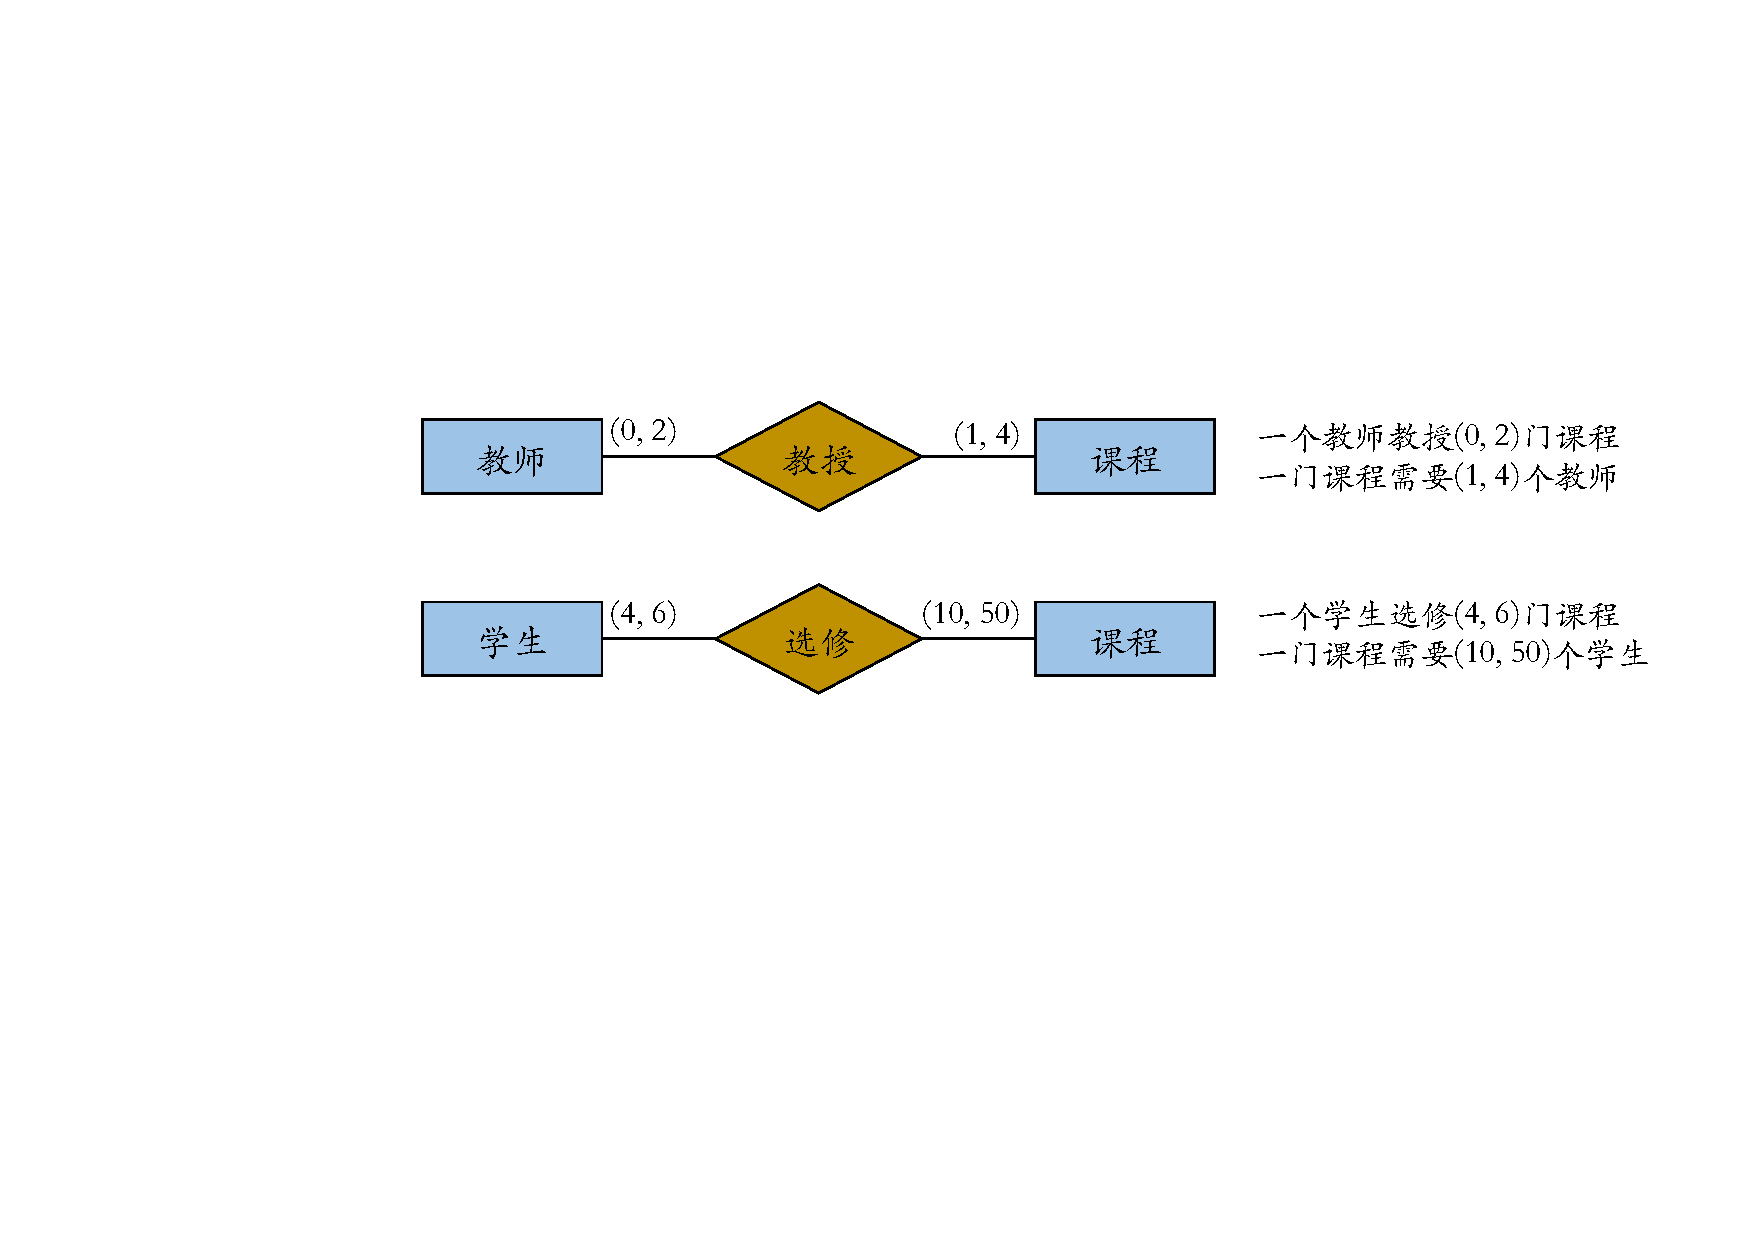
\includegraphics[width=.8\textwidth]{figure/联系的势.pdf}
    \caption{联系的势}
\end{figure}

\section{ER设计实例}

\subsection{基于业务描述的ER设计实例}

\begin{example}
    考虑一个学校数据库, 它要存储以下信息:
    \begin{itemize}
        \item 教师: \underline{教工号}、教工名、职称;
        \item 项目: \underline{项目号}、项目名称、起始年份、资助额;
        \item 学生: \underline{学号}、学生名、年龄、学位;
        \item 一个教工可以负责多个项目;
        \item 每个项目只能有一个负责人;
        \item 一个老师可以参与多个项目;
        \item 一个学生只能参与一个项目;
        \item 一个项目可以有多个学生和老师参与.
    \end{itemize}
\end{example}

\begin{figure}[H]
    \centering
    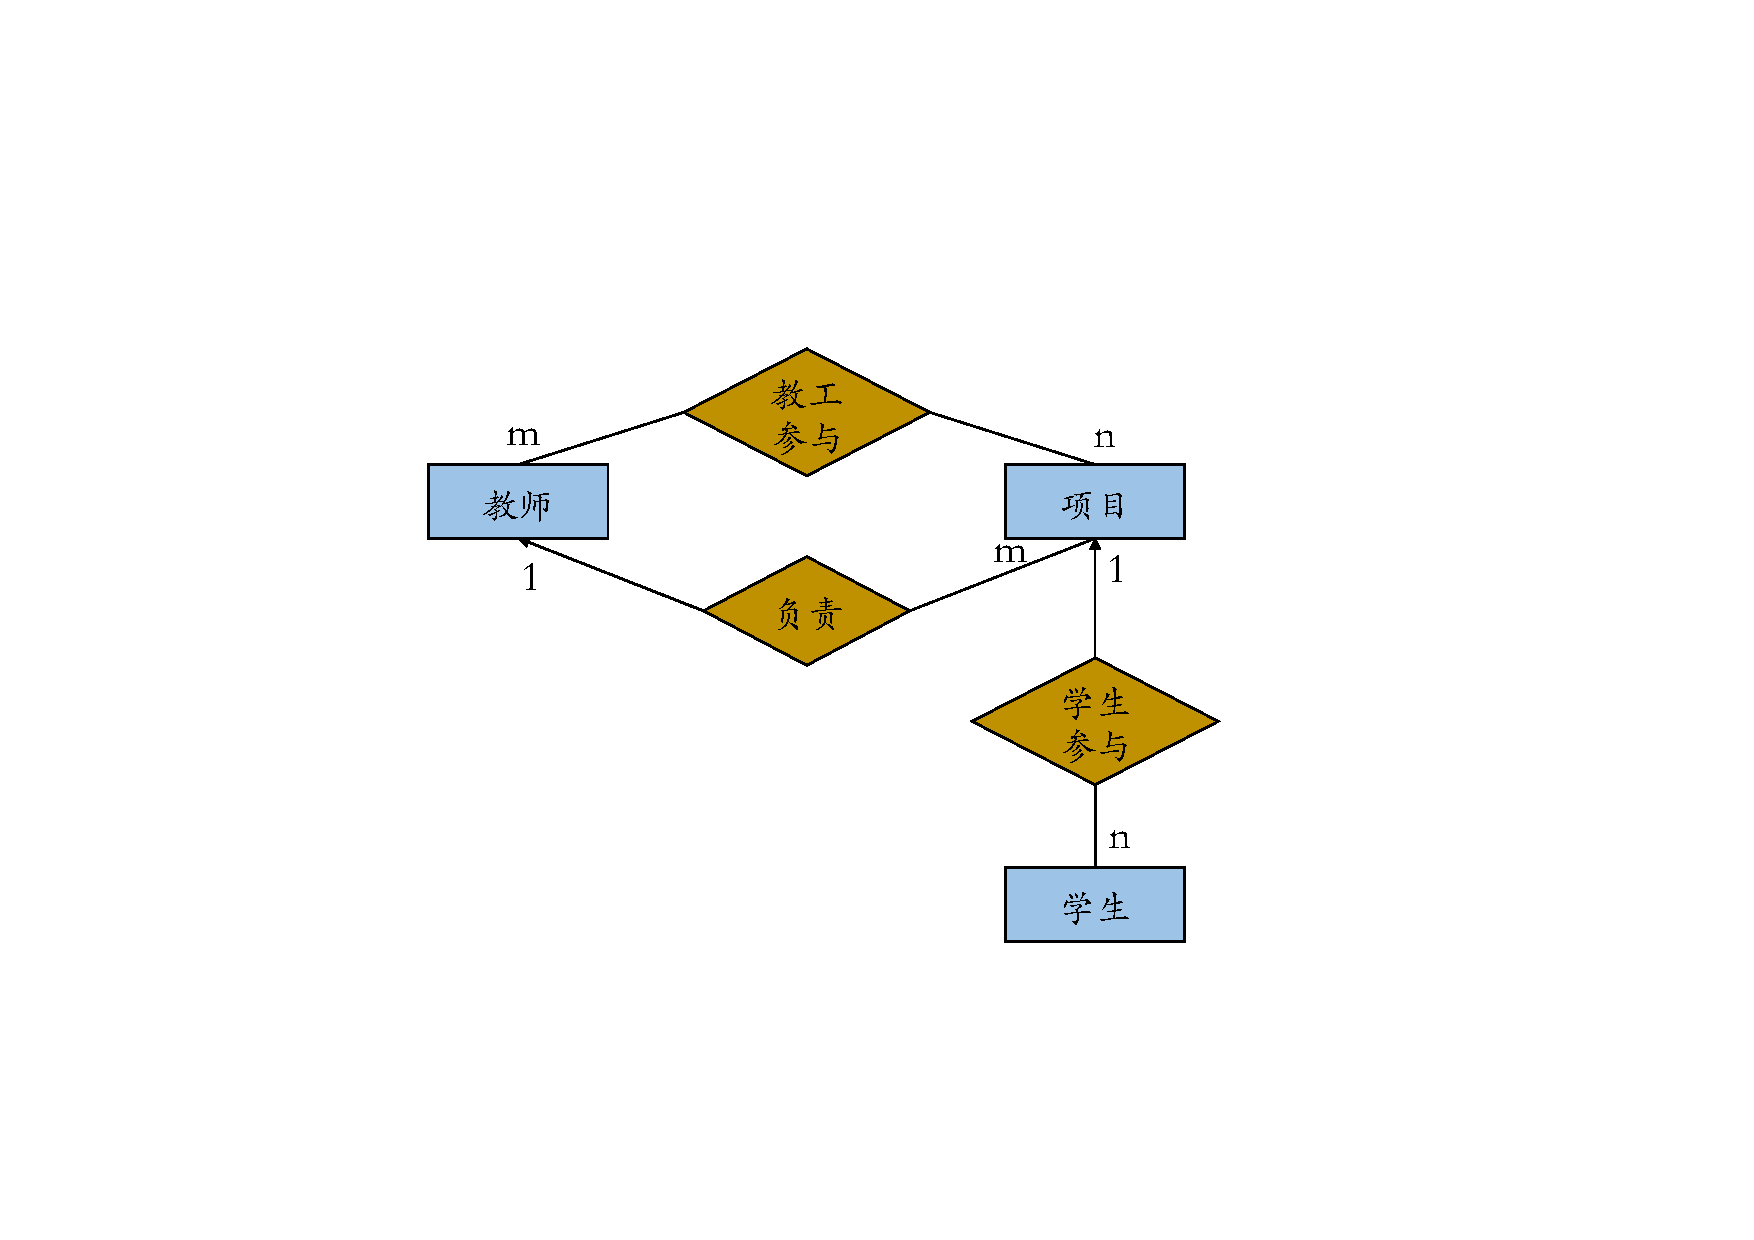
\includegraphics[width=.5\textwidth]{figure/ER实例1.pdf}
    \caption{基于业务描述的ER设计实例}
\end{figure}

\subsection{由业务单据生成ER模型}

\begin{figure}[H]
    \centering
    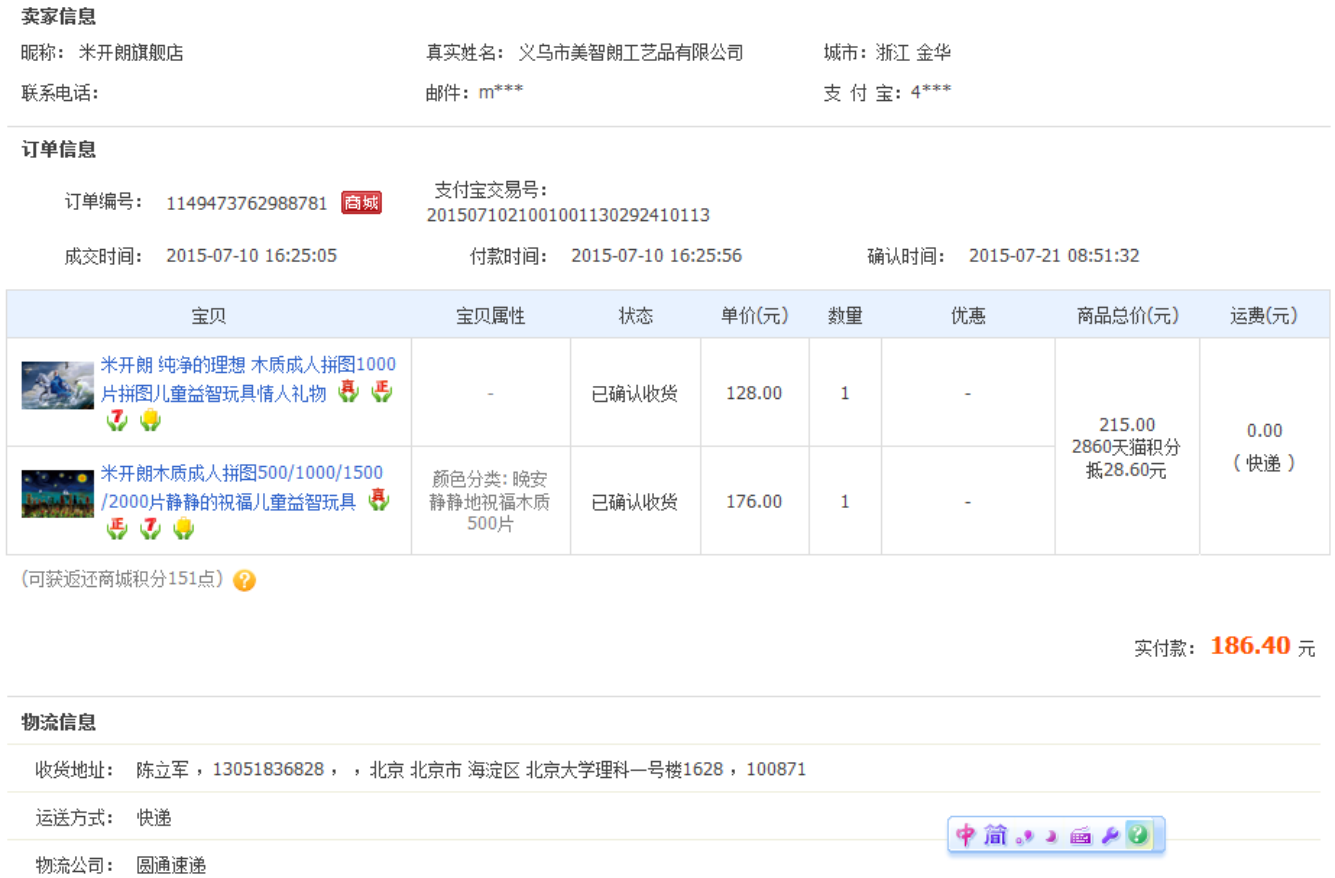
\includegraphics[width=.7\textwidth]{figure/ER实例2.png}
    \caption{订单}
\end{figure}

\begin{figure}[H]
    \centering
    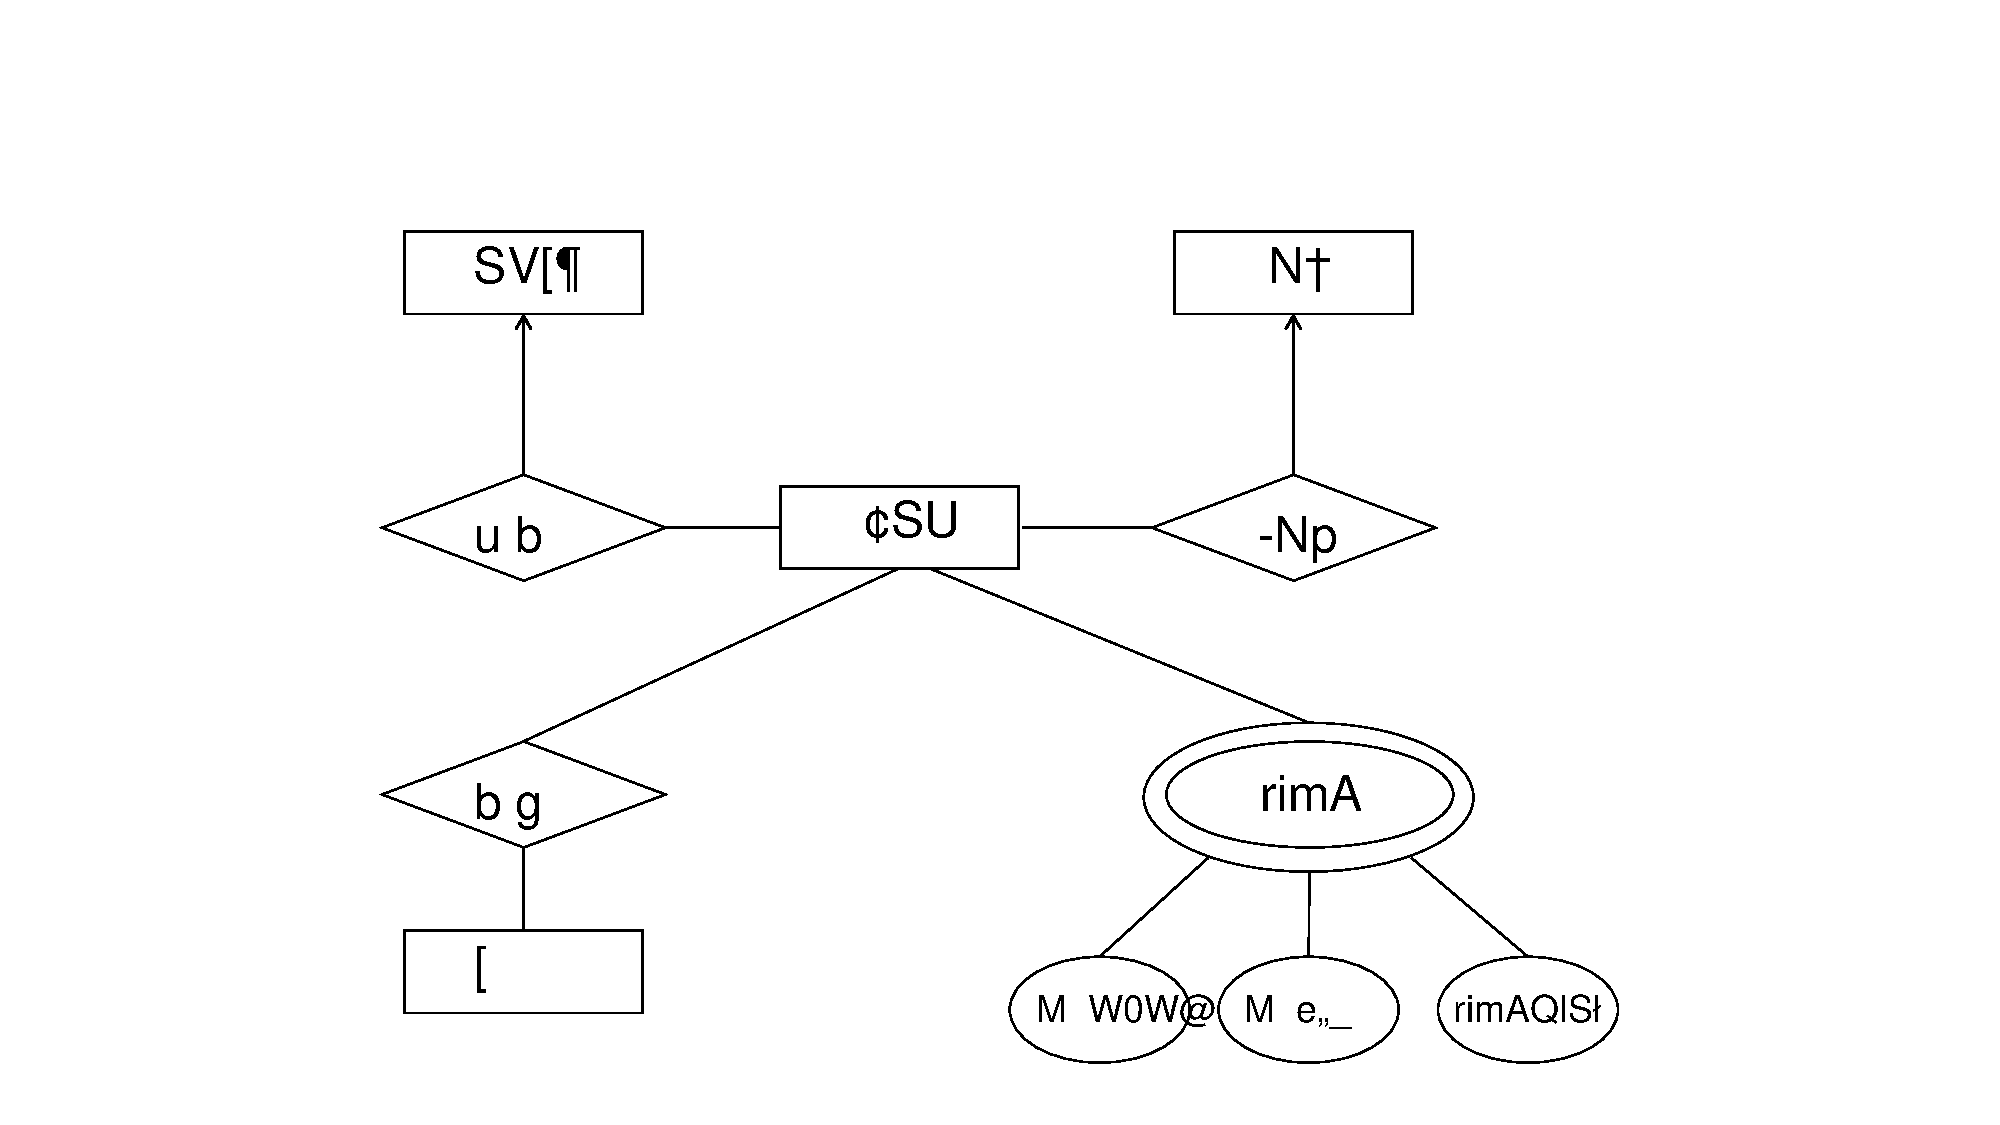
\includegraphics[width=.6\textwidth]{figure/ER实例3.pdf}
    \caption{由业务单据生成ER模型}
\end{figure}

\section{其他概念术语}

\begin{definition}[参与 (Participation)]
    实体集之间的关联称为参与, 即实体参与联系.
    \begin{itemize}
        \item $E$全部参与$R$: 实体集$E$中的每个实体都参与到联系集$R$中的至少一个联系.
        \item $E$部分参与$R$: 实体集$E$中只有部分实体参与到联系集$R$中的联系.
    \end{itemize}
\end{definition}

\begin{figure}[H]
    \centering
    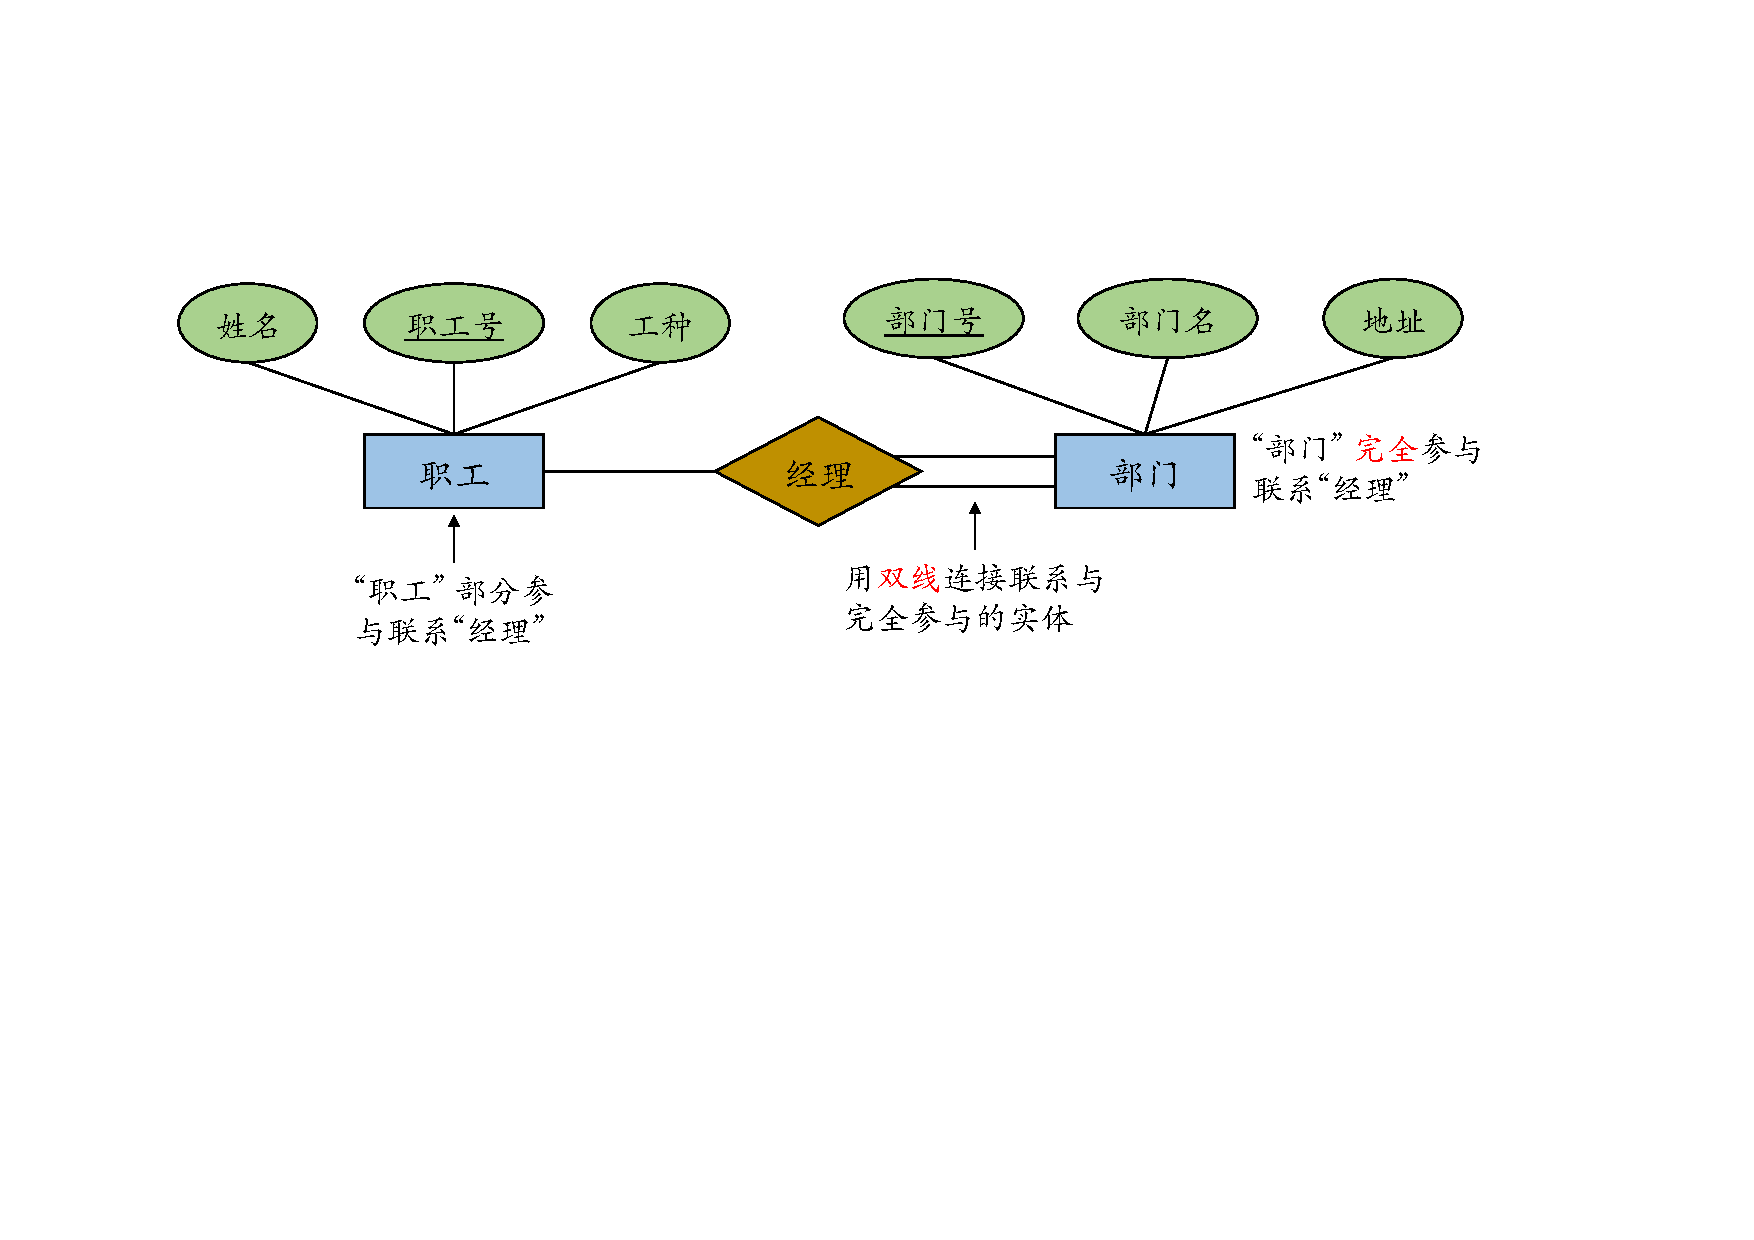
\includegraphics[width=.8\textwidth]{figure/参与.pdf}
    \caption{参与的ER图表示}
\end{figure}

\begin{definition}[角色 (Role)]
    实体在联系中的作用称为实体的角色. 对于一元联系, 为区别各实体参与联系的方式, 需要显式指明其角色. 如图\ref{n-ary-link}.
\end{definition}

\begin{definition}[存在依赖 (Exisitence Dependency)]
    $x$存在依赖于$y$意味着实体$x$的存在依赖于$y$, $y$称为支配实体, $x$称为从属实体.
\end{definition}

\begin{figure}[H]
    \centering
    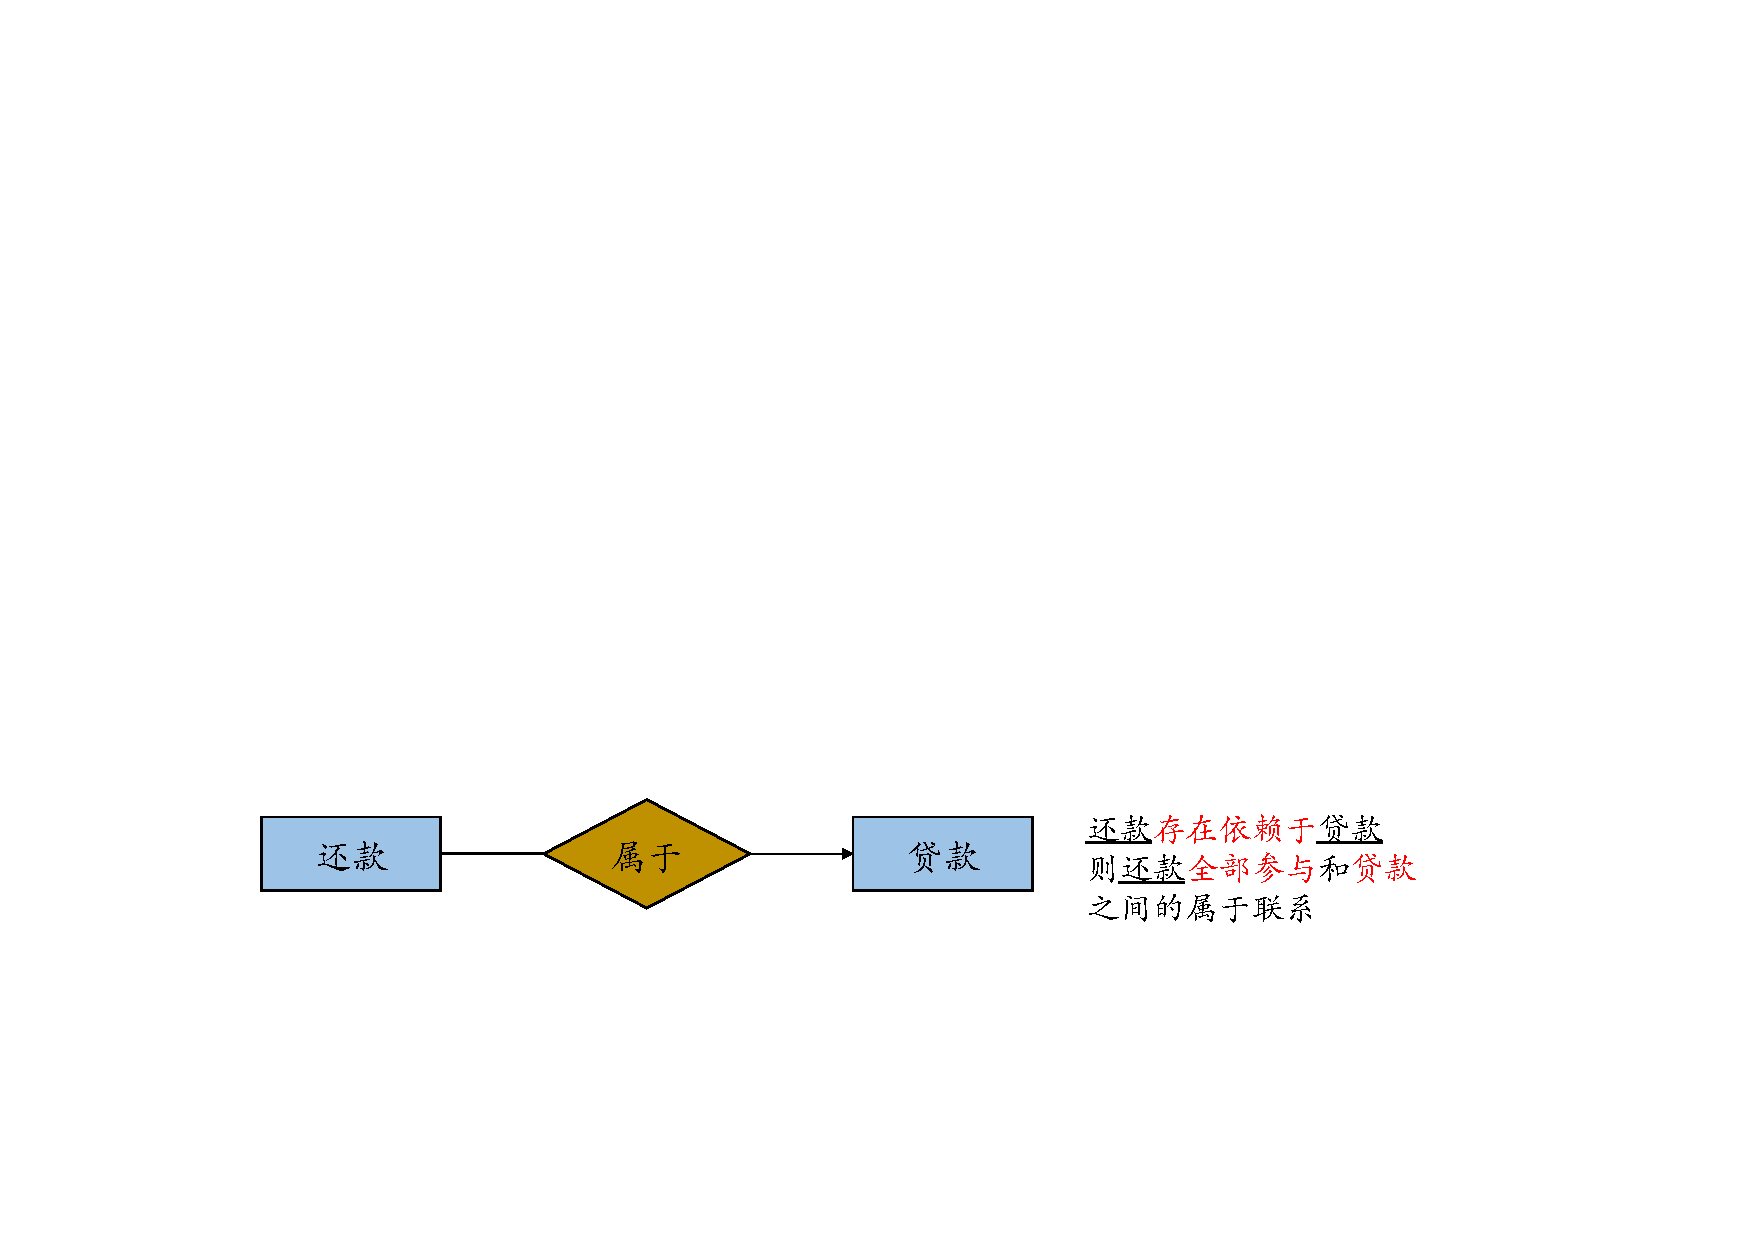
\includegraphics[width=.8\textwidth]{figure/存在依赖.pdf}
    \caption{存在依赖}
\end{figure}

复合实体. 一个 M:N 联系分解成两个 1:M. (了解即可.)

\section{扩展ER特性}

\begin{definition}[弱实体集 (weak entity set)]
    没有足够的属性以形成主码的实体集称为弱实体集.
\end{definition}

\begin{definition}[标识性联系 (identifying relationship)]
    弱实体集与其标识实体集相连的联系称为标识性联系 (identifying relationship). 其实就是弱实体集和强实体集的那一个联系.
\end{definition}

\begin{remark}
    弱实体集必然存在依赖于强实体集, 但是\textcolor{red}{存在依赖并不总会导致一个弱实体集}, 从属实体集可以有自己的主码.
\end{remark}

\begin{definition}[分辨符 (Discriminator)]
    弱实体集中用于区别依赖于某个特定强实体集的属性集合, 也称作部分码 (partial key).
\end{definition}

\textcolor{red}{!!!!!! 弱实体集的主码 = 强实体集的主码 + 弱实体集的分辨符}

\begin{figure}[H]
    \centering
    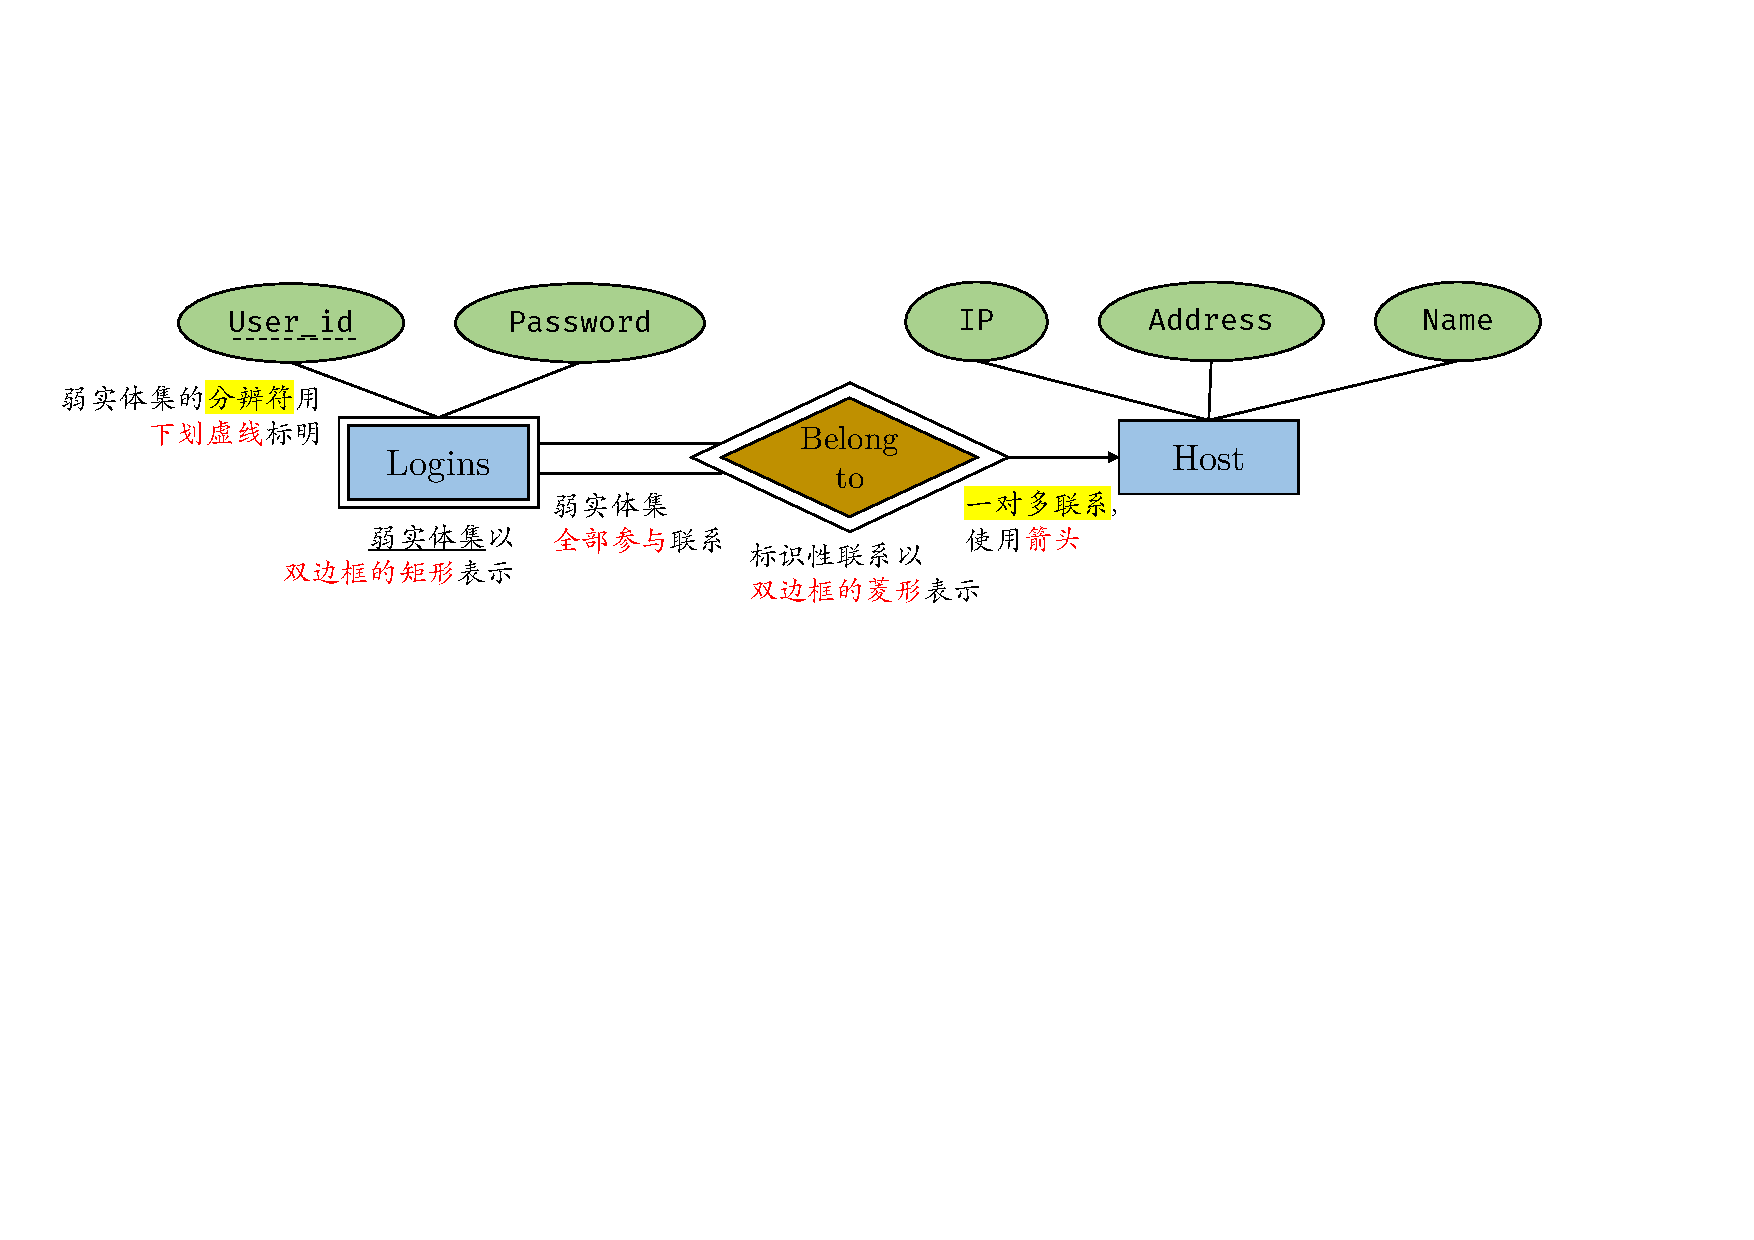
\includegraphics[width=\textwidth]{figure/弱实体集.pdf}
    \caption{弱实体集的ER表示}
\end{figure}

\begin{remark}
    何时引入弱实体集?
    \begin{itemize}
        \item 作为层次结构的一部分.
        \item 实体集的一些多值、复合属性可以抽取出来作为弱实体集.
        \item 如果弱实体集不但参与和强实体集之间的标识性联系, 
        而且参与和其它实体集的联系, 或者弱实体集本身含有很多属性, 则将其表述为弱实体集.
    \end{itemize}
\end{remark}

\begin{figure}[H]
    \centering
    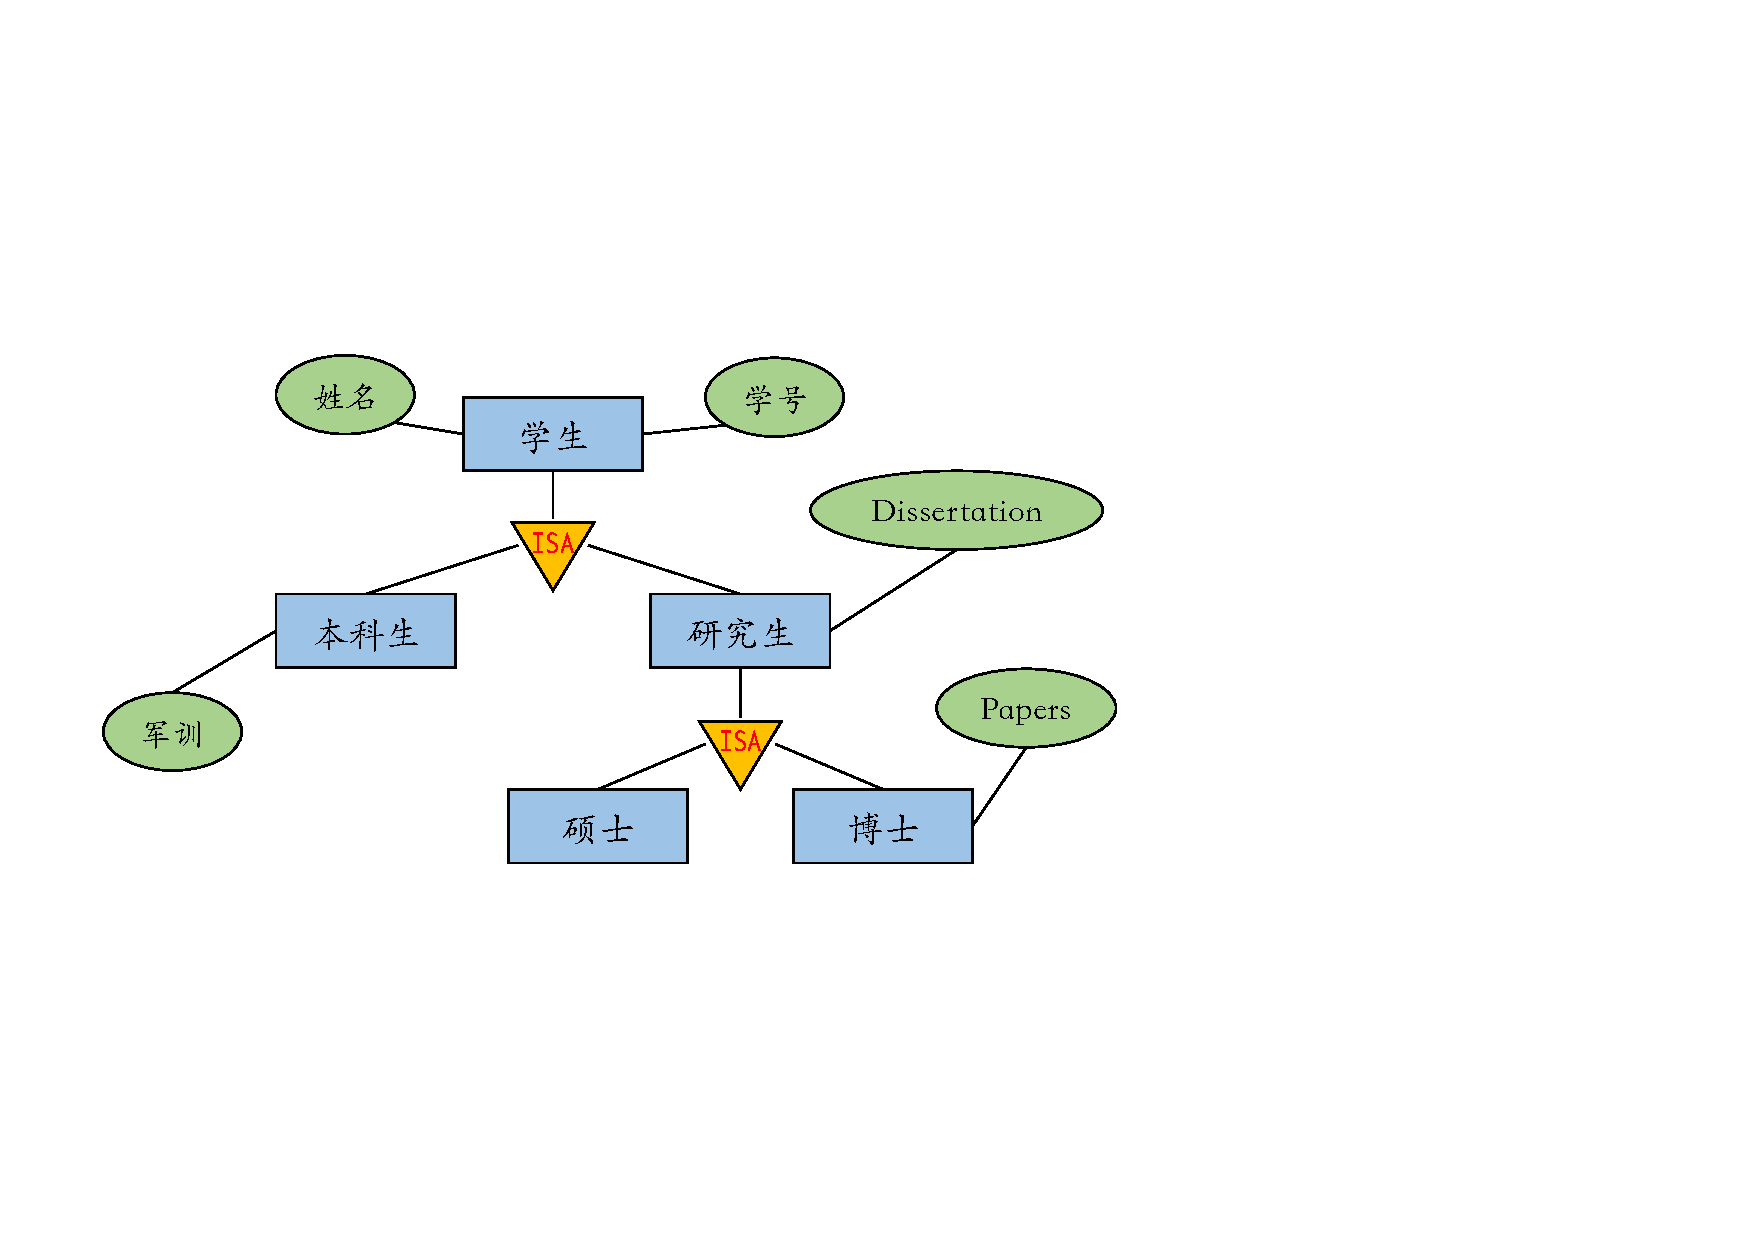
\includegraphics[width=.6\textwidth]{figure/特化.pdf}
    \caption{特化的ER表示}
\end{figure}

\begin{definition}[特化]
    实体集中某些子集具有区别于该实体集内其它实体的特性,可以根据这些差异特性对实体集进行分组,这一分组的过程称作特化. 标识为 ISA 的三角形. ISA = “is a”.
\end{definition}

\begin{definition}[概化]
    概化是高层实体集与一个或多个底层实体集的包含关系. 得到的 E-R 图和特化得到的 E-R 图是一样的, 只不过是自底向上.
\end{definition}

\begin{itemize}
    \item 层次结构(Hierarchy): 实体集作为低层实体集只能参与到一个ISA联系中.
    \item 格结构(Lattice): 低层实体集可以参与到多个ISA联系中.
\end{itemize}

\begin{figure}[H]
    \centering
    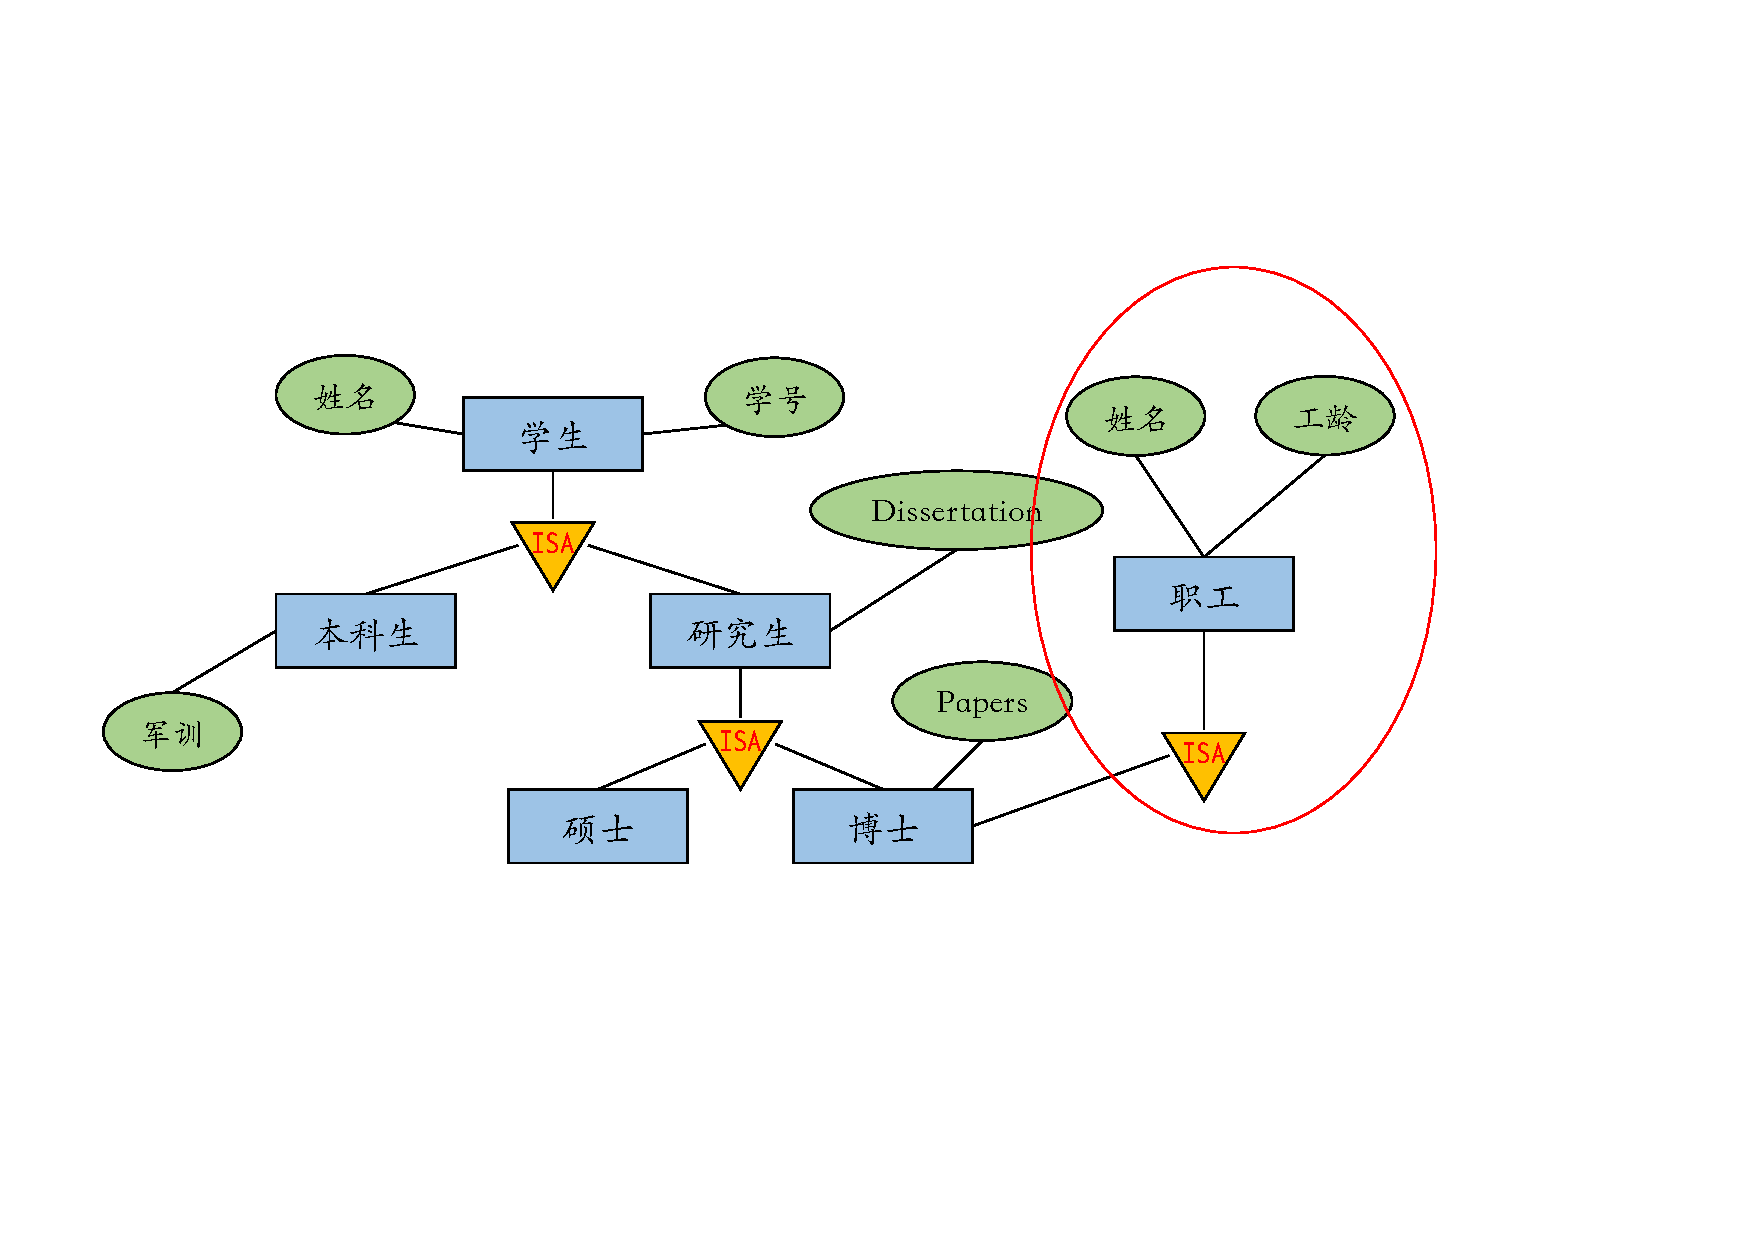
\includegraphics[width=.7\textwidth]{figure/格结构.pdf}
    \caption{格结构}
\end{figure}

概化中的成员身份:
\begin{itemize}
    \item 不相交的 (Disjoint): 一个实体至多属于一个低层实体集. e.g., 学生只能参加一个项目组, 学生就是不相交成员身份.
    \item 有重叠的 (Overlapping): 同一实体可同时属于同一概化的多个低层实体集. e.g., 老师可以参加多个项目组, 老师就是有重叠成员身份.
\end{itemize}

概化中的全部性约束: 确定高层实体集中的一个实体是否\textbf{必须}属于至少一个低层实体集.
\begin{itemize}
    \item 全部的 (Total): 每个高层实体必须属于一个低层实体集. e.g., 学生必须属于本科生或者研究生其中一种.
    \item 部分的 (Partial): 允许一些高层实体不属于任何低层实体集. e.g., 学生可以不属于任何的项目组.
\end{itemize}

\begin{definition}[聚集]
    两个先后动作的序列.
\end{definition}

\begin{figure}[H]
    \centering
    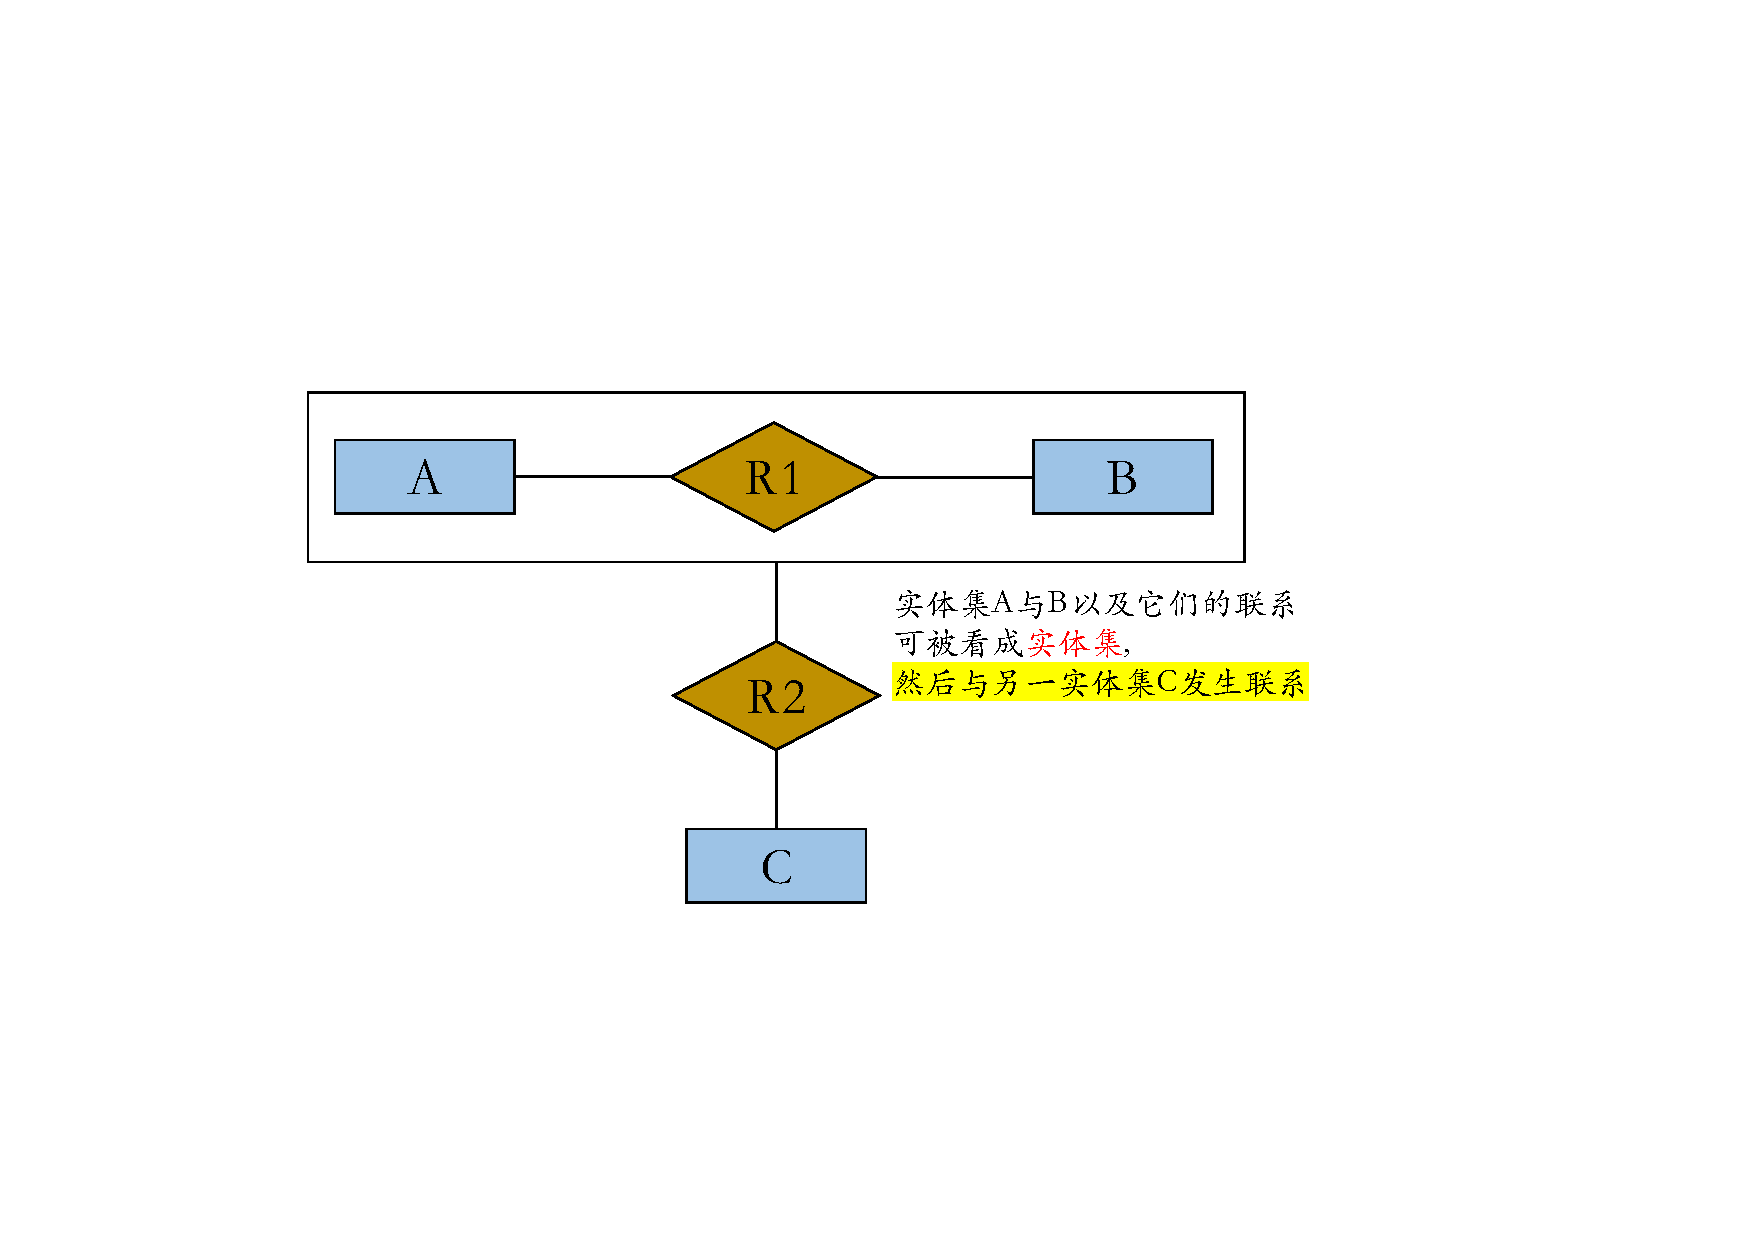
\includegraphics[width=.5\textwidth]{figure/聚集.pdf}
    \caption{聚集的ER表示}
\end{figure}


\begin{example}
    能否把多元联系转换为若干个二元联系?
\end{example}

新构建一个\textcolor{red}{标识实体集}$E$, 构造三个新联系集$R_A, R_B, R_C$, 对于每个$(a_i,b_i,c_i)\in R$, 在$E$中创建一个$e_i$, 然后在$R_A, R_B, R_C$中分别加入联系$(e_i,a_i),(e_i,b_i),(e_i,c_i)$.

这样的转换并无实际意义.

\begin{figure}[H]
    \centering
    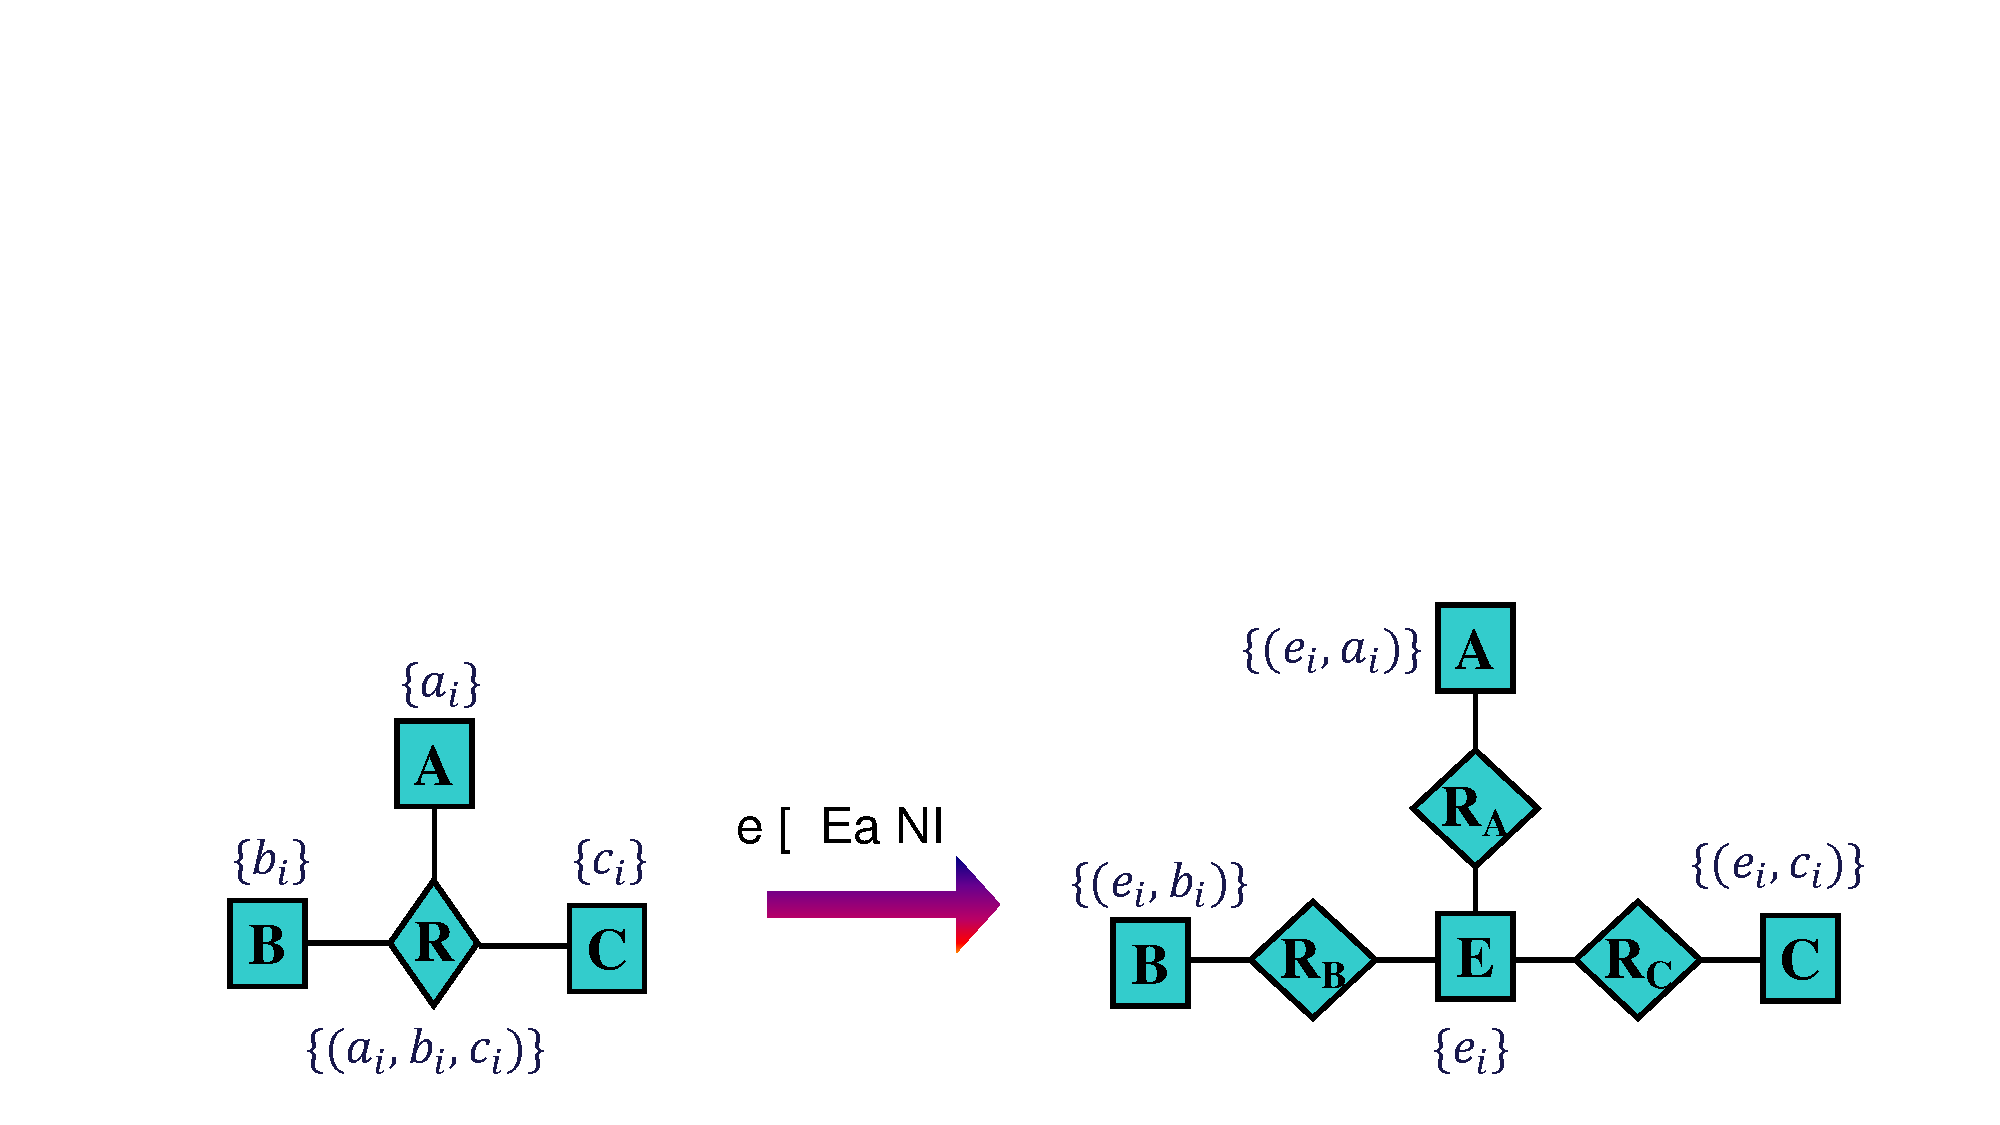
\includegraphics[width=.8\textwidth]{figure/无意义转换.pdf}
    \caption{无意义的转换}
\end{figure}

\section{概念数据库设计过程}

\begin{itemize}
    \item 局部ER模式设计.
    \item 全局ER模式设计.
    \item 全局ER模式优化.
\end{itemize}

\section{ER模型向关系模式的转换}

\begin{enumerate}
    \item 实体 $\to$ 关系.
    \item 属性 $\to$ 关系的属性.
    \begin{enumerate}
        \item 复合属性定义为视图, 或者由应用定义, 这里摊平即可.
        \item 多值属性 $\to$ 新的关系 + (取值+所在实体的码)
    \end{enumerate}
    \item 一对多联系 $\to$ 将单方参与实体的码作为多方参与实体的属性.
    \item 多对多联系 $\to$ 将联系定义为新的关系, 属性为参与双方的码.
    \item 一对一联系 $\to$ 若联系双方均部分参与, 则将联系定义为一个新的关系, 属性为参与双方的码. 全部参与同一对多.
    \item 弱实体集 $\to$ 弱实体集所对应的关系的码由弱实体集本身的分辨符再加上所依赖的强实体集的码.
    \item 概化 $\to$ 高层实体集和低层实体集分别转为表, 低层实体集所对应的关系包括高层实体集的码.
    \item 聚集 $\to$ 实体集A与B及其联系R被抽象成实体集C, C与另一实体集D构成联系S, 则S的码由C和D的码构成.
\end{enumerate}

\section{关系模式向ER的转换}

!识别关系间的重合属性.


 % !UNIFINSHED FOR LAST 3 SECTORS.

\chapter{关系模型}

\section{关系基本概念}

\begin{definition}[域(Domain)]
具有相同数据类型的一组值的集合.
如整数集合、字符串集合、全体学生集合.
\end{definition}

\begin{definition}[笛卡尔积(Cartesian Product)]
一组域$D_1,D_2,...,D_n$的\textcolor{red}{笛卡尔积}为:
\begin{align*}
    D_1\times D_2\times \cdots\times D_n = \{(d_1,d_2,...,d_n)|d_i\in D_i, i=1,2,...,n\}.
\end{align*}
笛卡尔积的元素$(d_1,d_2,...,d_n)$称作$n$元组(tuple).

元组的每一个值$d_i$被称作分量(component).

若$D_i$的基数为$m_i$, 则笛卡尔积的基数为$\prod_{i=1}^{n}m_i$.
\end{definition}

\begin{definition}[关系]
笛卡尔积$D_1\times D_2\times \cdots\times D_n$的子集称作在域$D_1,D_2,...,D_n$上的\textcolor{red}{关系}. 用$R(D_1,D_2,...,D_n)$表示. $R$是关系的名字, $n$是关系的度或目.

关系是笛卡尔积中\textcolor{red}{有意义}的子集.
\end{definition}

关系的性质:
\begin{enumerate}
    \item $P_1$: 列是同质的, 是同一类型的数据, 即每一列中的分量来自同一域.
    \item $P_2$: 不同的列可以来自同一域, 每列必须有不同的属性名. (一元联系、类型相同的属性)
    \item $P_3$: 行列的顺序无关紧要.
    \item $P_4$: 任意两个元组不能完全相同 (集合内不能有相同的两个元素)
    \item $P_5$: 每一分量必须是不可再分的数据, 称其为作满足第一范式(1NF)的关系. 
\end{enumerate}

\section{关系模型三要素}

关系模型的三要素:
\begin{enumerate}
    \item 数据结构.
    \item 数据操作.
    \item 数据完整性.
\end{enumerate}

\subsection{数据结构}

关系模型的数据结构就是\textcolor{red}{关系}: 实体集和联系都表示为关系.

\begin{definition}[候选码(Candidate Key)]
关系中的一个属性组, 其值能唯一标识一个元组. 
若从属性组去掉任何一个属性, 它就不具有这一性质了, 这样的属性组称为候选码.
\end{definition}

\begin{definition}[主属性]
任何一个候选码中的属性被称为主属性.
\end{definition}

\begin{definition}[主码(Priamry Key, PK)]
进行数据库设计时, 从一个关系的多个候选码中选定一个作为主码.
\end{definition}

\begin{definition}[外码(Foreign Key, FK)]
关系$R$中的一个属性组, 它不是$R$的码, 但它与另一个关系$S$的码相
对应, 称这个属性组为$R$的外码.
\end{definition}

\begin{definition}[关系模式]
关系的描述, 记为$R(A_1,A_2,...,A_n)$, 包括:
\begin{enumerate}
    \item 关系名、关系中的属性名.
    \item 属性向域的映像, 通常说明为属性的类型、长度等.
    \item 属性间的数据依赖关系, 比如在特定的时间和教室只能安排一门课.
\end{enumerate}
关系模式是稳定的.
\end{definition}

\begin{definition}[关系]
关系是某一时刻对应某个关系模式的内容(元组的集合). 关系是某一时刻的值, 是随时间不断变化的.
\end{definition}

\begin{definition}[关系型数据库]
\begin{enumerate}
    \item 型: 关系模式的集合, 数据库描述. 数据库的内涵(Intension).
    \item 值: 是某一时刻关系的集合. 数据库的外延(Extension).
\end{enumerate}
\end{definition}

\subsection{数据操作}

关系操作是集合操作. 操作的对象及结果都是集合. 是一次一集合 (Set-at-a-time)的方式.

非关系型的数据操作方式是一次一记录(Record-at-a-time).

关系数据语言的特点:
\begin{enumerate}
    \item 一体化: 对象单一, 都是关系, 因此操作符也单一
    \item 非过程化: 用户只需提出“做什么” , 无须说明“怎么做”. 存取路径的选择和操作过程由系统自动完成
    \item 面向集合的存取方式: 一次一关系.
\end{enumerate}

抽象的关系模型查询语言:
\begin{enumerate}
    \item 关系代数. 过程查询语言.
    \item 关系演算: 元组关系演算、域关系演算. 非过程查询语言.
\end{enumerate}

SQL(介于关系代数和关系验算之间, by IBM)、QUEL(基于 Codd 提出元组关系演算语言ALPHA)、QBE.

\subsection{数据完整性}

\begin{definition}[关系模型完整性]
关系模型完整性由三部分组成:
\begin{enumerate}
    \item 实体完整性
    \item 参照完整性
    \item 用户定义完整性
\end{enumerate}
\end{definition}

\begin{definition}[实体完整性]
关系的主码中的属性值不能为空值. (保证其实体存在.)
\end{definition}

\begin{definition}[参照完整性]
如果关系$R_2$的外码$F_k$与关系$R_1$的主码$P_k$相对应, 
则$R_2$中每个元组的$F_k$值或者等于$R_1$中某个元组的$P_k$值, 或者为空值.

如果关系$R_2$的某个元组$t_2$参照了关系$R_1$的某个元组$t_1$, 则$t_1$必须存在, 
也即必须与客观存在的实体发生联系.
\end{definition}

\begin{figure}[H]
    \centering
    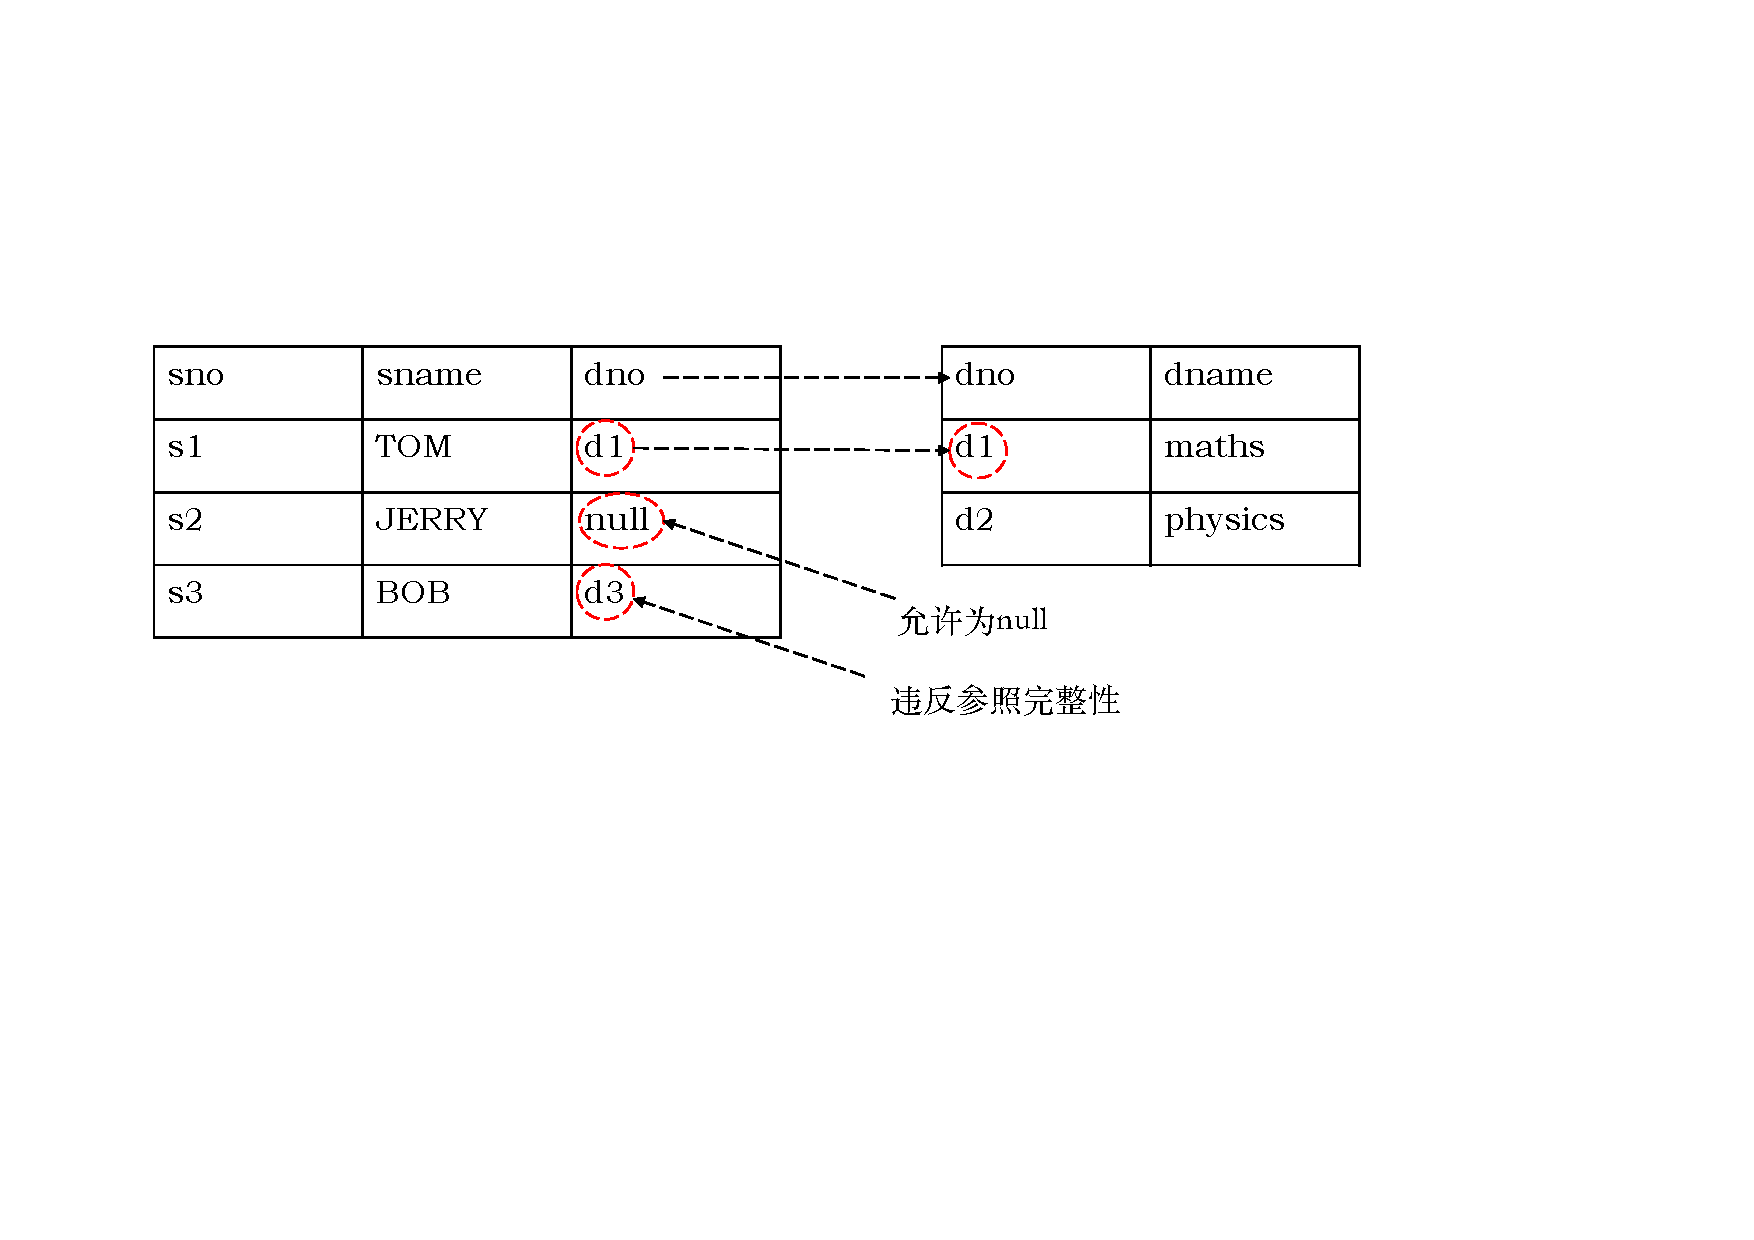
\includegraphics[width=.6\textwidth]{./figure/参照完整性.pdf}
    \caption{参照完整性}
\end{figure}

\begin{definition}[用户完整性]
用户针对具体应用环境定义的完整性约束条件.
\end{definition}

实体完整性和参照完整性由系统自动支持, 系统提供定义和检验用户定义的完整性的机制.

\section{关系代数运算}

\begin{figure}[H]
    \centering
    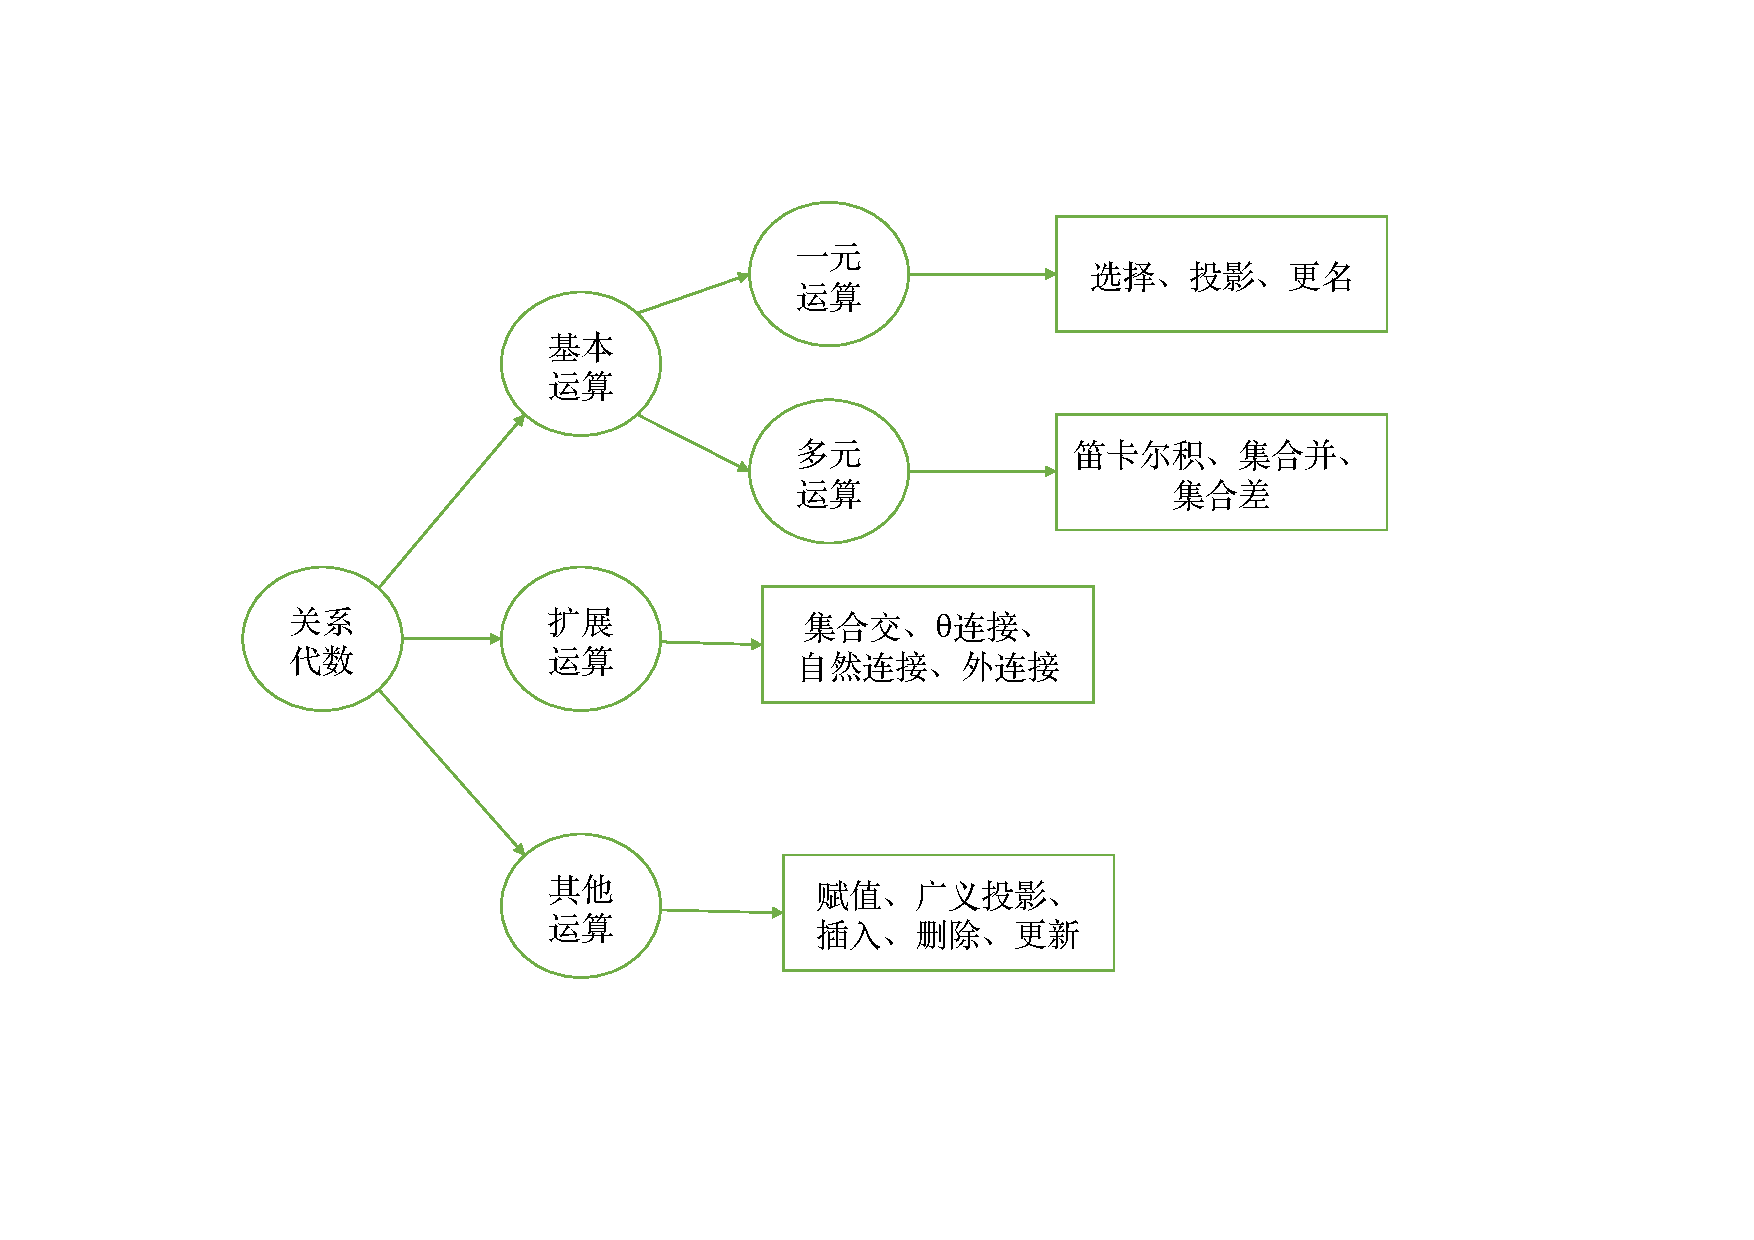
\includegraphics[width=.6\textwidth]{./figure/关系代数.pdf}
    \caption{关系代数示意图}
\end{figure}

\subsection{基本关系代数运算}

\subsubsection{一元运算}

\begin{definition}[选择运算]
在关系中选择给定条件的元组(行角度):
\begin{align*}
    \sigma_F(R)=\{t|t\in R,F(t)=\text{true}\}.
\end{align*}
$F$由逻辑运算符连接算术表达式而成.
\end{definition}

\begin{definition}[投影运算]
从关系中取若干列组成新的关系(从列的角度):
\begin{align*}
    \Pi_A(R) = \{t[A]|t\in R\}, A \subseteq R.
\end{align*}
\end{definition}

投影的结果要去掉相同的行:
\begin{figure}[H]
    \centering
    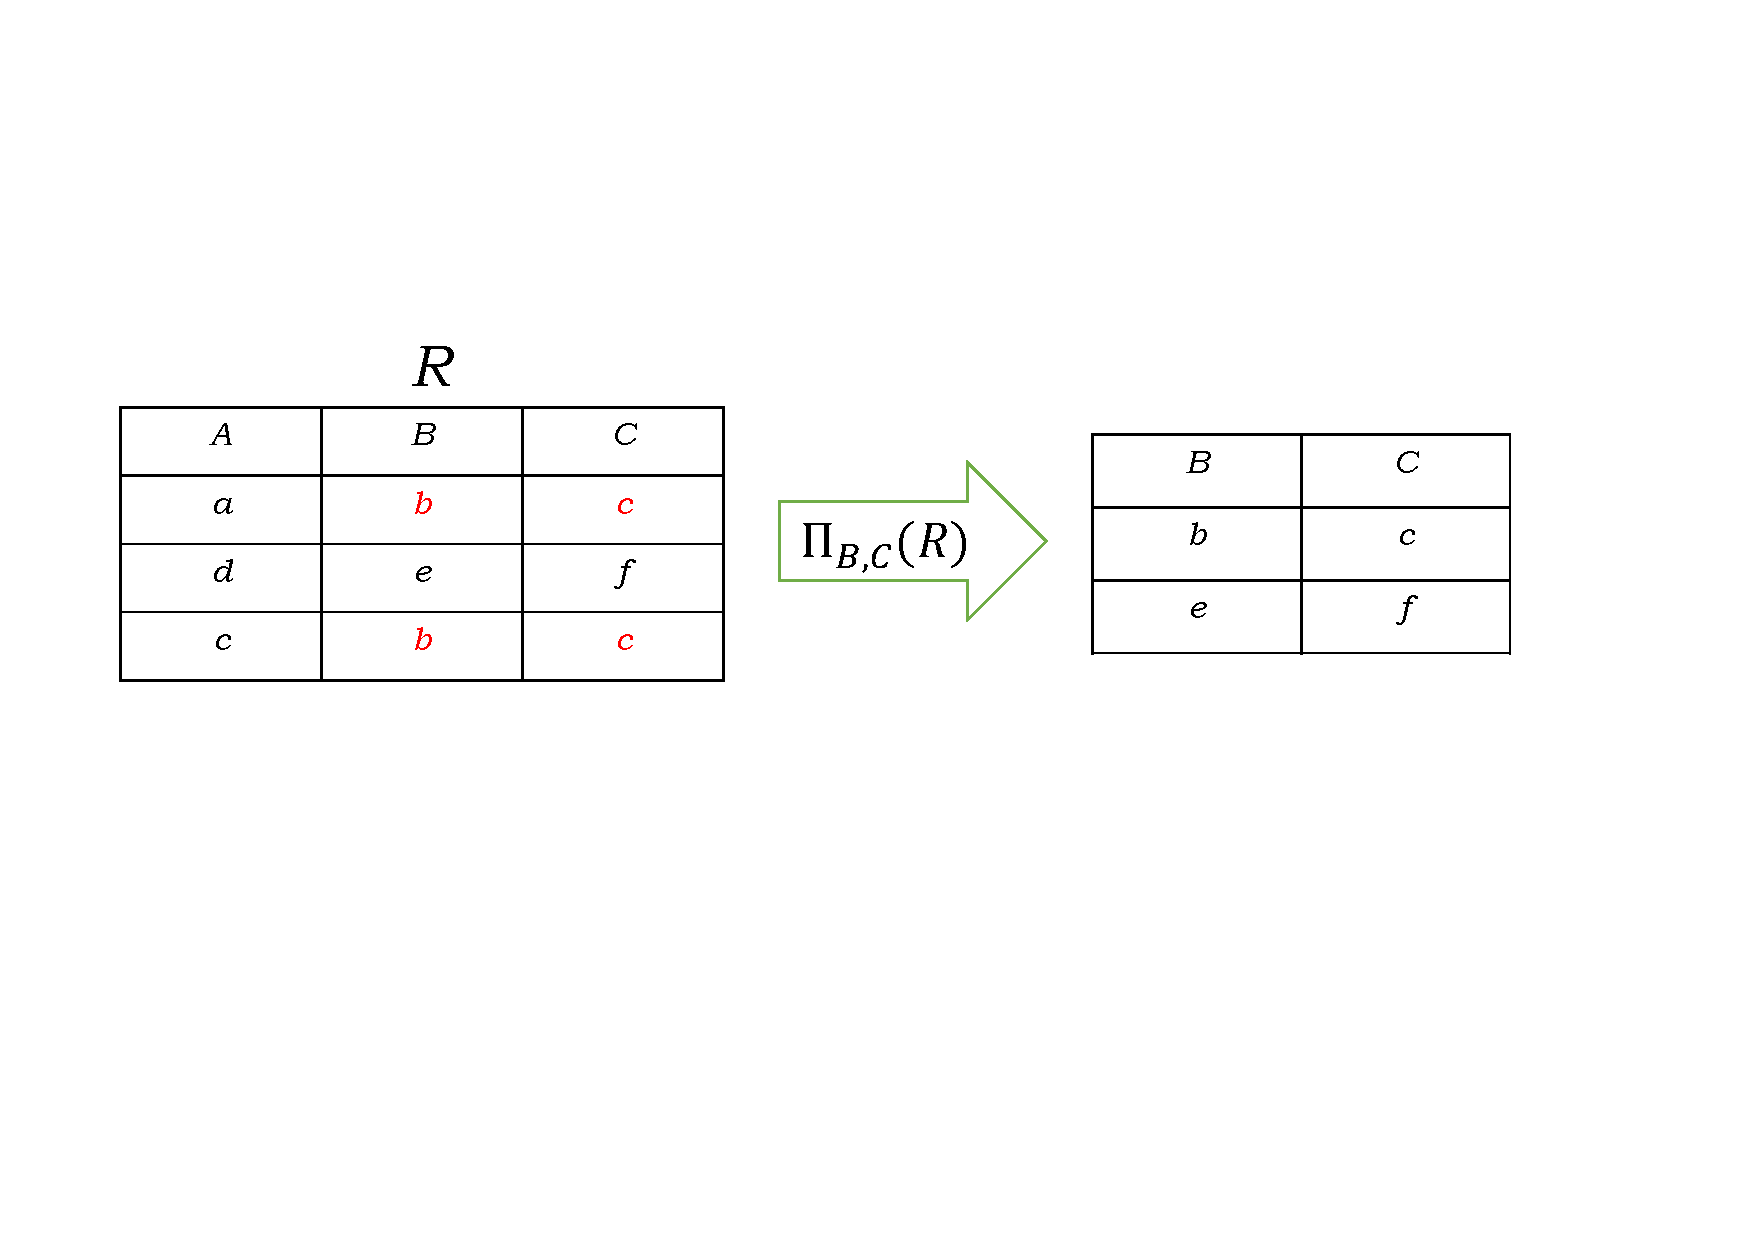
\includegraphics[width=.7\textwidth]{./figure/投影.pdf}
    \caption{投影运算要去掉相同的行}
\end{figure}

\begin{definition}[更名运算]
将关系$R$更名为$S: \rho_S(R)$; 将计算表达式$E$更名为关系$S: \rho_{S(A_1,A_2,...,A_n)}(E)$.
\begin{enumerate}
    \item 将更名运算施加到关系上, 得到具有不同名字的同一关系
    \item 当同一关系多次参与同一运算时需要更名
\end{enumerate}
\end{definition}

\subsubsection{多元运算}

\begin{definition}[并运算]
\begin{align*}
    R\cup S =\{r|r\in R\lor r \in S\}.
\end{align*}
关系$R$和$S$进行并运算的前提是它们必须是相容的.
\begin{enumerate}
    \item 关系$R$和$S$必须是同元的, 其属性数目必须相同.
    \item 对$\forall i$, $R$的第$i$个属性和$S$的第$i$个属性的域必须相同.
\end{enumerate}
\end{definition}

\begin{example}
选修了001号或002号课程的学生号.
\begin{align*}
    &\Pi_{\text{sno}}(\sigma_{\text{cno}=001\lor \text{cno}=002}(\text{SC})) \\
    &\Pi_{\text{sno}}(\sigma_{\text{cno}=001}(\text{SC})\lor \sigma_{\text{cno}=002}(\text{SC}))
\end{align*}
\end{example}

\begin{definition}[差运算]
\begin{align*}
    R-S =\{r|r\in R\land r \not\in S\}.
\end{align*}
\end{definition}

\begin{example}
求选修了001号但未选修002号课程的学生号.
\begin{align*}
    &\Pi_{\text{sno}}(\sigma_{\text{cno}=001}(\text{SC})) - \Pi_{\text{sno}}(\sigma_{\text{cno}=002}(\text{SC})) \\
   &\Pi_{\text{sno}}(\sigma_{\text{cno}=001\lor \text{cno}\neq 002}(\text{SC}))
\end{align*}
\end{example}

\begin{definition}[连串(Concatenation)]
$r=(r_1,r_2,...,r_n)$, $s=(s_1,s_2,...,s_m)$, $r$与$s$的连串定义为:
\begin{align*}
    \widehat{rs} = (r_1,r_2,...,r_n,s_1,s_2,...,s_m).
\end{align*}
\end{definition}

\begin{definition}[笛卡尔积]
\begin{align*}
    R\times S=\{\widehat{rs}|r\in R\land s\in S\}.
\end{align*}
\begin{itemize}
    \item $R\times S$的度为$R$和$S$的度之和.
    \item $R\times S$的元组个数为$R$和$S$的元组个数之积.
\end{itemize}
\end{definition}

\begin{example}
求选修c1课程的学生姓名.
\end{example}

\begin{figure}[H]
    \centering
    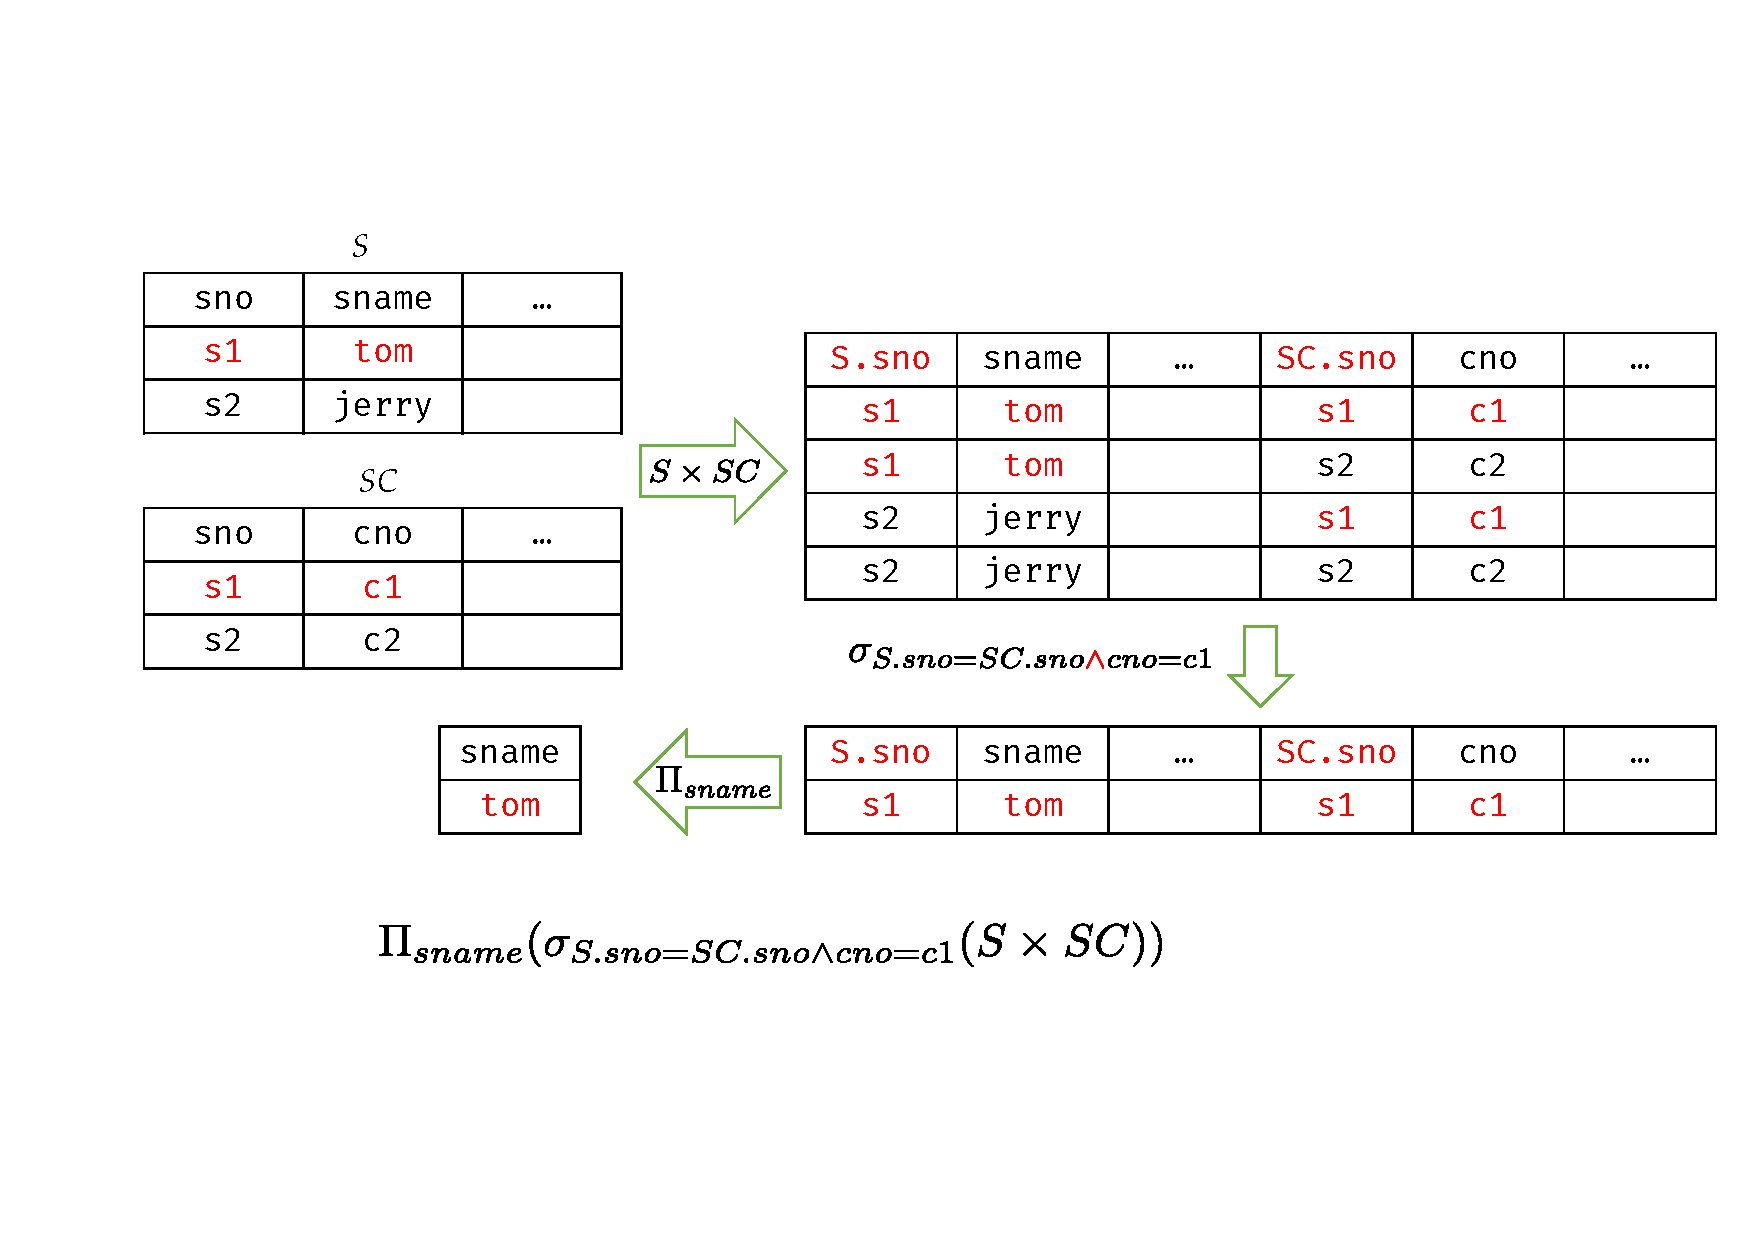
\includegraphics[width=.8\textwidth]{./figure/笛卡尔积的使用.pdf}
    \caption{笛卡尔积的使用}
\end{figure}

\begin{example}
求数学成绩比王红同学高的学生姓名.
\end{example}
\begin{align*}
    \Pi_{S.\text{姓名}}\left(\sigma_{R.\text{姓名}=\text{王红}\land R.\text{课程}=\text{数学}\land S.\text{课程}=\text{数学} \land R.\text{成绩} < S.\text{成绩}} (R\times \rho_S(R))\right)
\end{align*}

\subsection{扩展关系代数运算}

\begin{definition}[交运算]
\begin{align*}
    R\cap S =\{r|r\in R\land r \in S\}.
\end{align*}
$R\cap S = R-(R-S)$.
\end{definition}

\begin{example}
求同时选修了001号和002号课程的学生号.
\end{example}
\begin{align*}
    &\Pi_{\text{sno}}(\sigma_{\text{cno}=001}(\text{SC})) \cap \Pi_{\text{sno}}(\sigma_{\text{cno}=002}(\text{SC})) \\
    &\Pi_{\text{sno}}(\sigma_{\text{cno}=001\land \text{cno}=002}(\text{SC}))
\end{align*}

\begin{definition}[$\theta$连接]
从两个关系的广义笛卡儿积中选取给定属性间满足一定条件的元组:
\begin{align*}
    R \underset{{A\theta B}}{\bowtie} S = \{\widehat{rs}|r\in R \land s \in S \land r[A]\theta s[B]\}
    = \sigma_{r[A]\theta s[B]}(R\times S).
\end{align*}
\end{definition}

$A,B$为$R$和$S$上度数相等且可比的属性列, $\theta$为算术比较符.

\begin{example}
求数学成绩比王红同学高的学生姓名.
\end{example}
\begin{align*}
    \Pi_{S.\text{姓名}}\left(\sigma_{\text{课程}=\text{数学}\land \text{姓名}=\text{王红}}(R) \underset{R.\text{成绩}<S.\text{成绩}}{\bowtie}\sigma_{\text{课程}=\text{数学}}\rho_S(R)\right)
\end{align*}

\begin{definition}[等值连接]
$\theta$为等号的时候为等值连接.
\end{definition}

\begin{definition}[自然连接]
从两个关系的广义笛卡儿积中选取在相同属性列$B$上取值相等的元组, 并去掉重复的列:
\begin{align*}
    R \bowtie S = \{ \widehat{rs}[\bar{B}] | r \in R \land s \in S \land r[B]=s[B] \}.
\end{align*}
自然连接与等值连接不同: 自然连接中相等的分量必须是相同的属性组, 并且要在结果中去掉重复的属性, 而等值连接则不必.
\end{definition}

\begin{example}
求出001号学生所在系的名称:
\begin{align*}
    &\Pi_{\text{dname}}(\sigma_{\text{sno}=001}(S\bowtie \text{Dept})) \\
    &\Pi_{\text{dname}}(\sigma_{\text{sno}=001}(S)\bowtie \text{Dept})
\end{align*}
\end{example}

\begin{figure}[H]
    \centering
    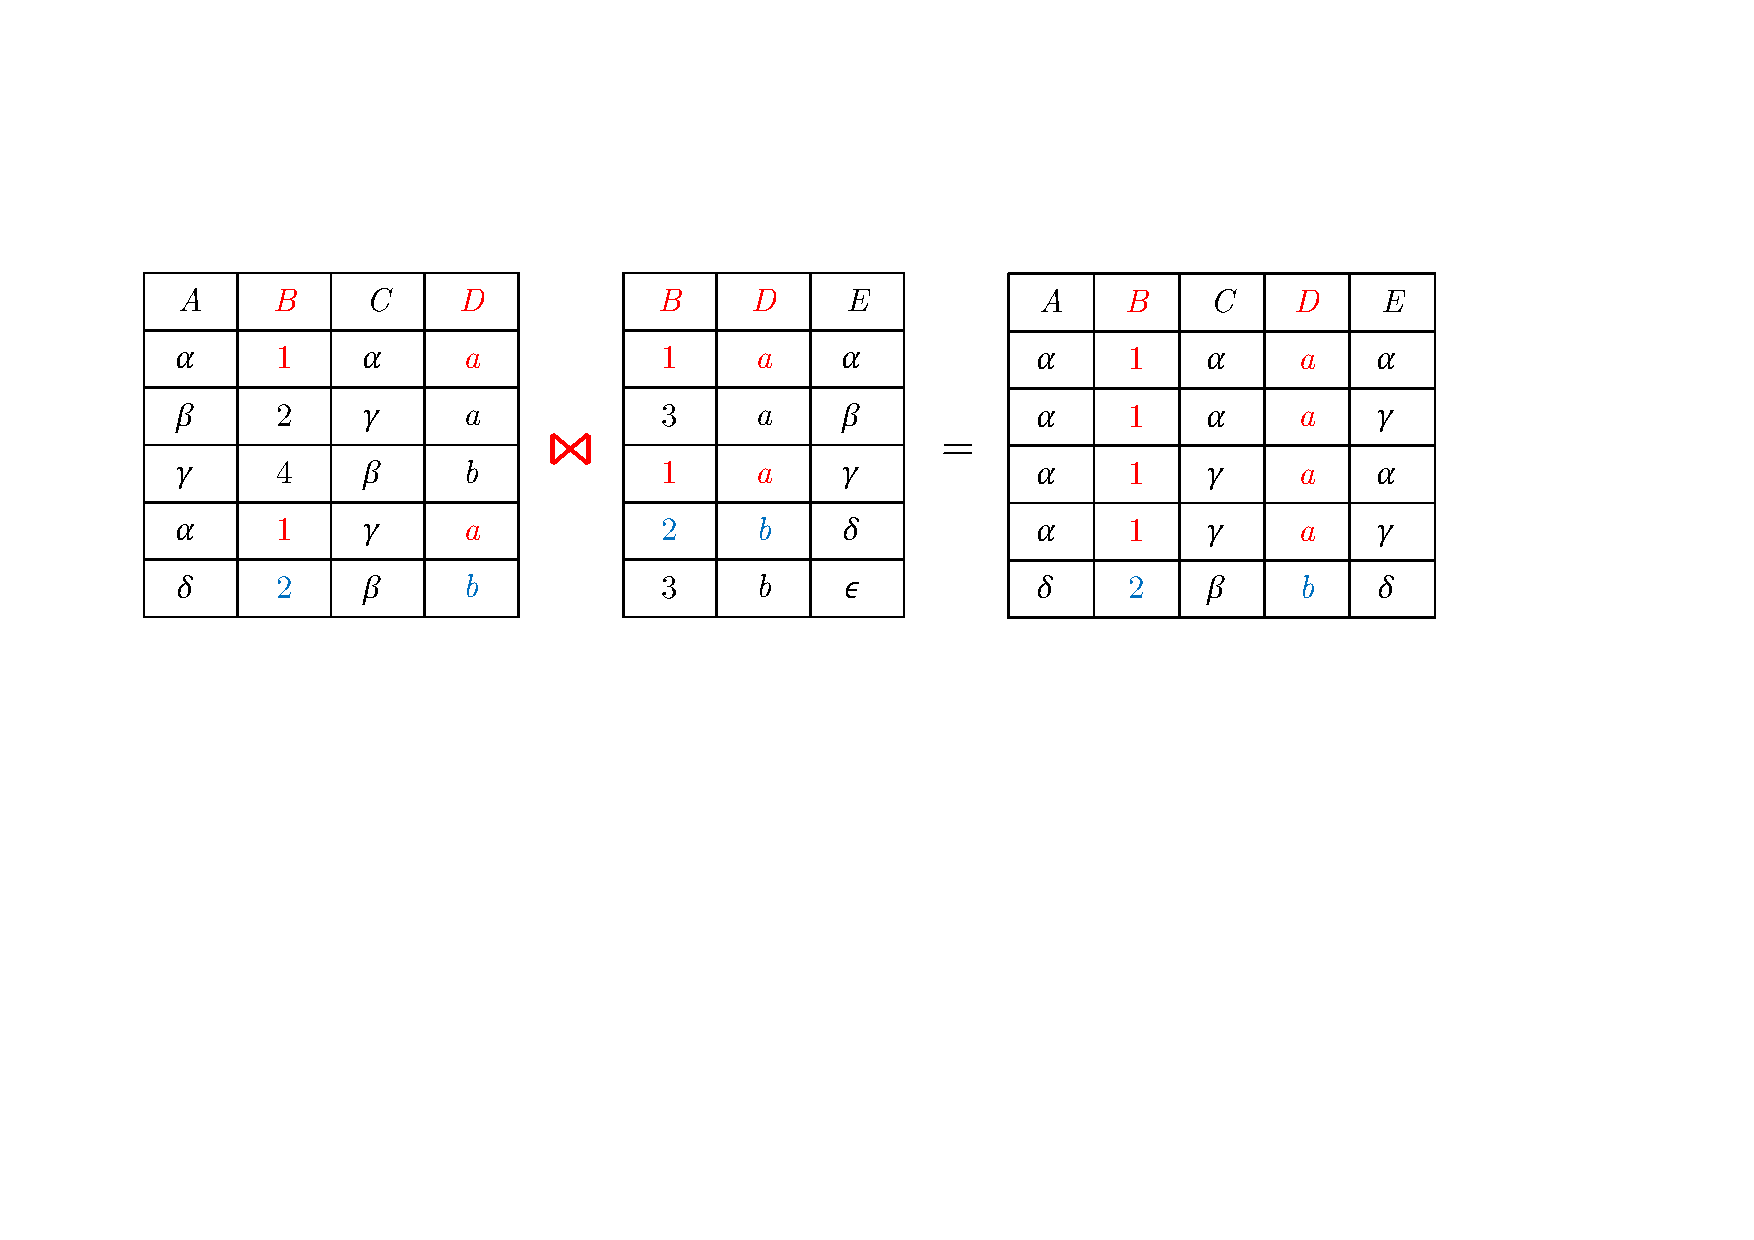
\includegraphics[width=.8\textwidth]{./figure/自然连接.pdf}
    \caption{自然连接例子}
\end{figure}

\begin{example}
关系$R(A,B)$, $S(A,C)$, $R$与$S$中元组个数分别为10, 15, 试填写下表.
\end{example}

\begin{table}[H]
\centering
\begin{tabular}{|c|c|c|c|}
\hline
条件 & 表达式 & 最小元组数 & 最大元组数 \\ \hline
\multirow{2}{*}{无任何条件} & $R \bowtie S$ & 0 & 150 \\ \cline{2-4}
 & $\Pi_A(R) \cup \Pi_A(S)$ & 1 & 25 \\ \hline
\multirow{2}{*}{A是R的主码} & $R \bowtie S$ & 0 & 15 \\ \cline{2-4}
 & $\Pi_A(R) \cup \Pi_A(S)$ & 10 & 25 \\ \hline
\multirow{2}{*}{\begin{tabular}[c]{@{}c@{}}A是R的主码\\ A是S的外码\end{tabular}} & $R \bowtie S$ & 15 & 15 \\ \cline{2-4}
 & $\Pi_A(R) \cup \Pi_A(S)$ & 10 & 10 \\ \hline
\end{tabular}
\caption{不同条件下的表达式及其元组数范围}
\end{table}

自然连接的问题: \textbf{因失配而发生信息丢失}.

\begin{definition}[外连接]
为避免自然连接时因失配而发生的信息丢失, 
可以假定往参与连接的一方表中附加一个取值全为空值的行, 
它和参与连接的另一方表中的任何一个未匹配上的元组都能匹配, 称之为外连接.

外连接 = 自然连接 + 未匹配元组(悬挂元组).

外连接的形式:
\begin{enumerate}
    \item 左外连接 = 自然连接 + 左侧表中未匹配元组. $\leftouterjoin$.
    \item 右外连接 = 自然连接 + 右侧表中未匹配元组. $\rightouterjoin$.
    \item 全外连接 = 左外连接 + 右外连接. $\fullouterjoin$.
\end{enumerate}
\end{definition}

\begin{figure}[H]
    \centering
    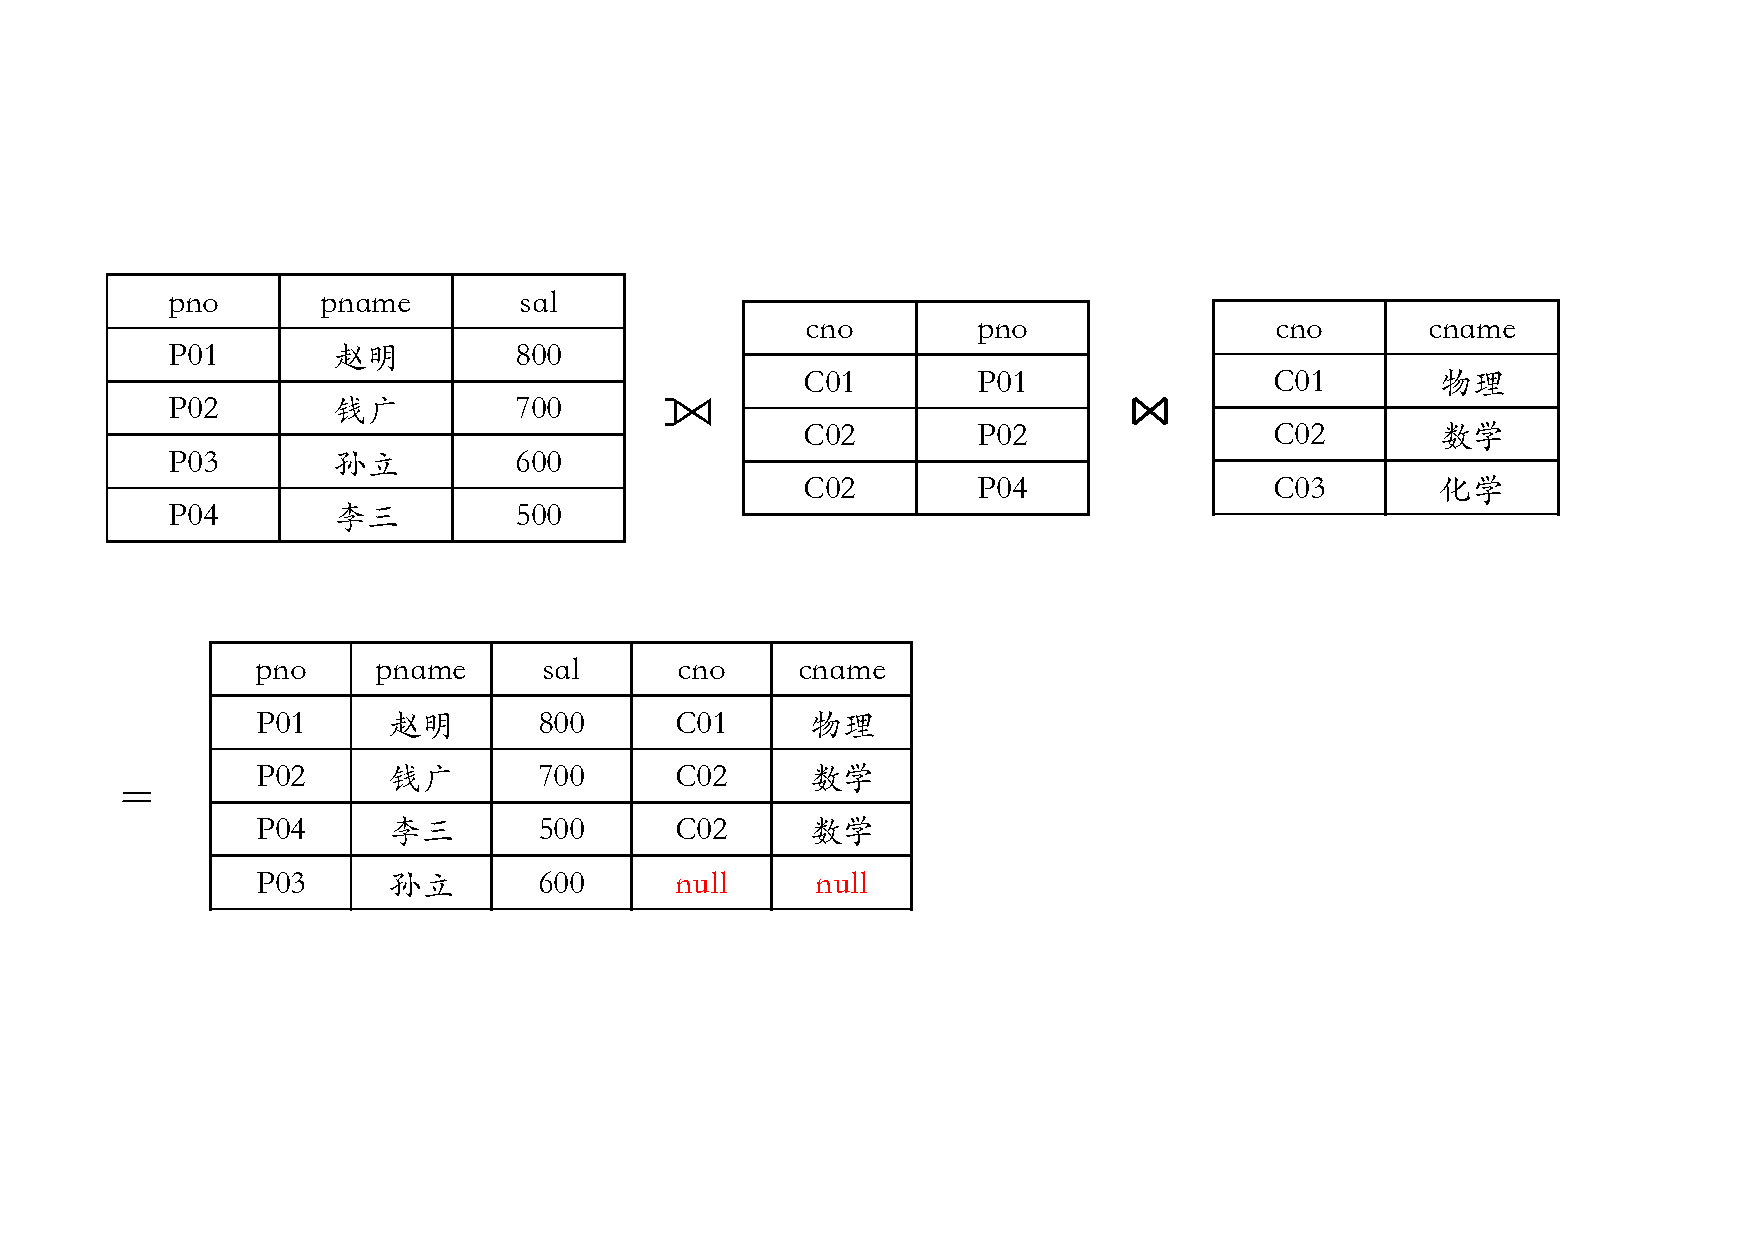
\includegraphics[width=.85\textwidth]{./figure/左外连接.pdf}
    \caption{左外连接示意图}
\end{figure}

外连接结合律不成立的反例:
\begin{figure}[H]
    \centering
    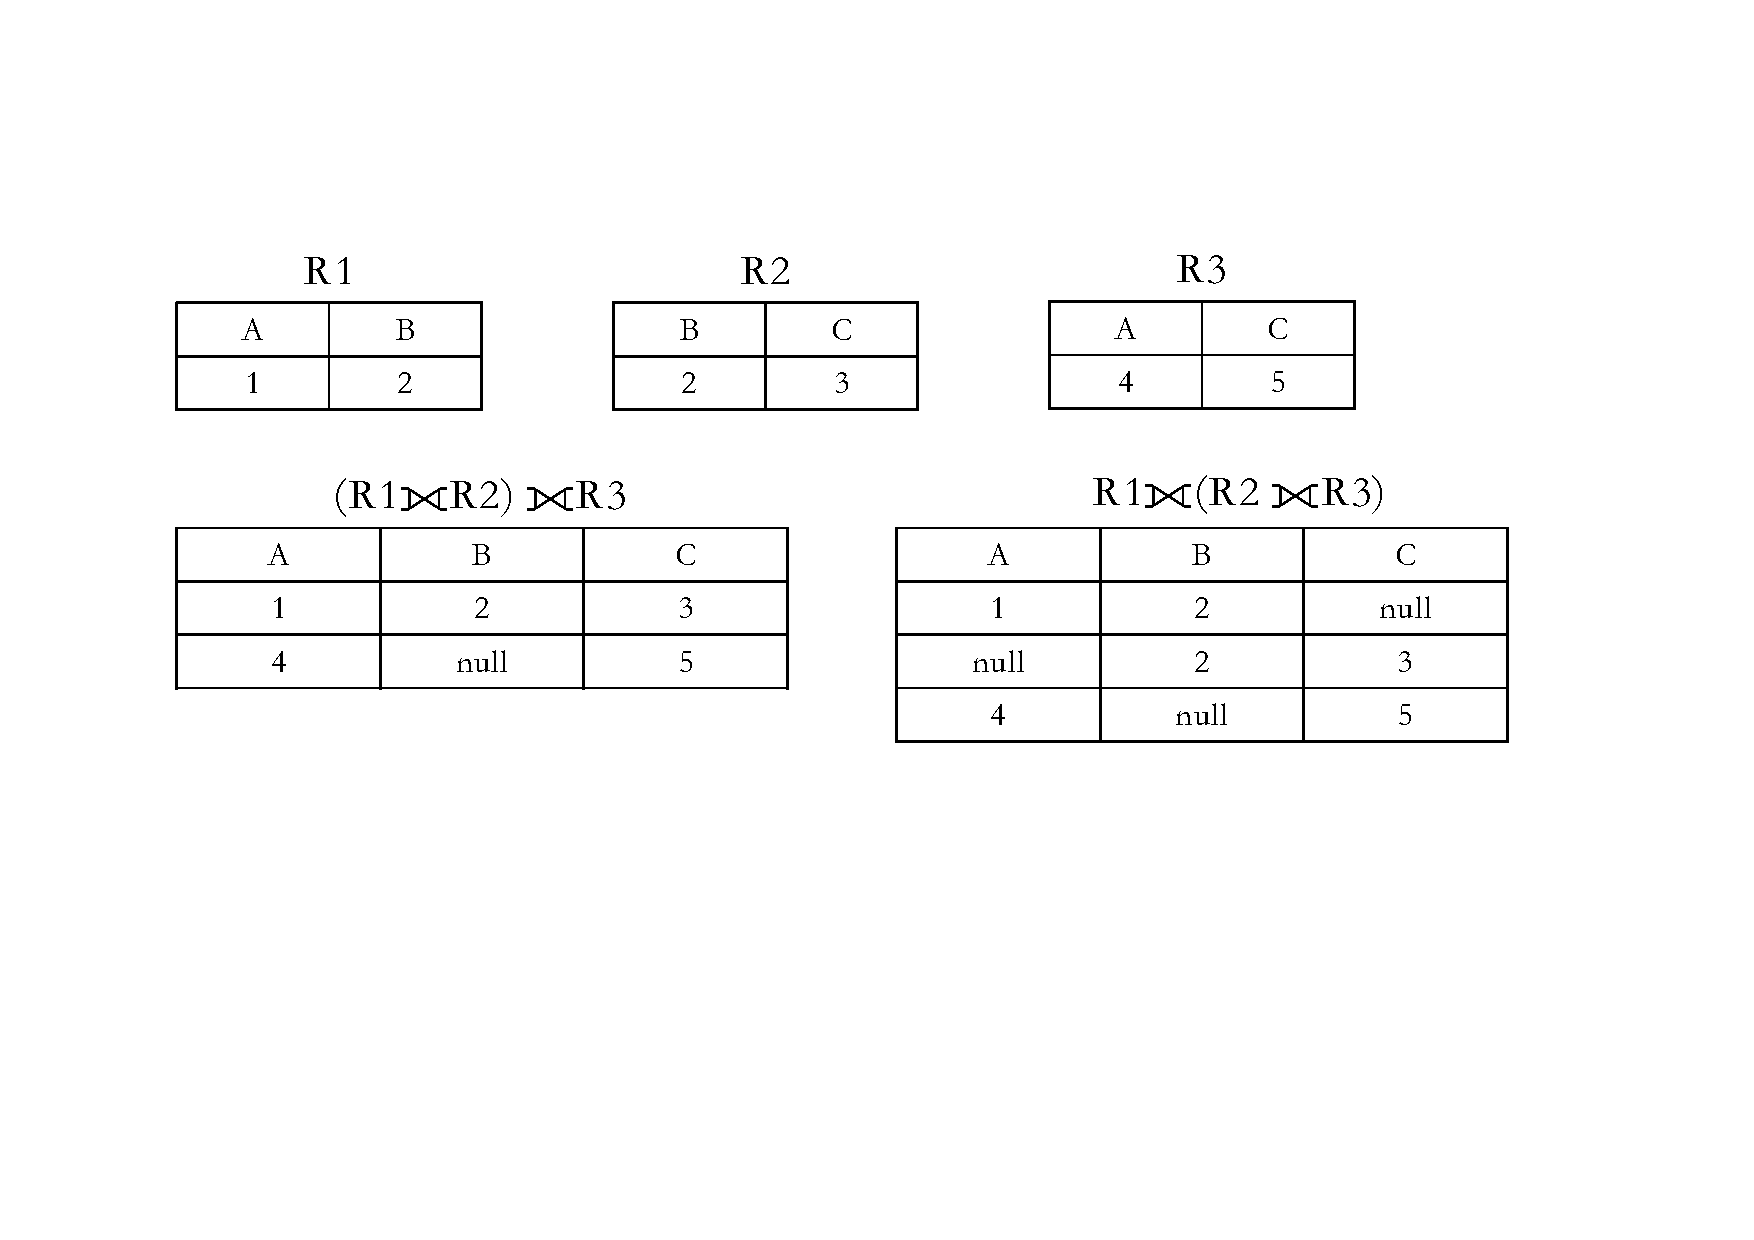
\includegraphics[width=.8\textwidth]{./figure/外连接结合律不成立.pdf}
    \caption{外连接结合律不成立的反例}
\end{figure}

\begin{definition}[半连接]
半连接(Semi-join)是一种用于优化查询的操作, 特别是在分布式数据库系统中. 
它主要用于减少数据传输量, 提高查询效率. 
半连接操作的目标是从两个关系(表)中返回第一个关系中的那些元组(行), 
这些元组与第二个关系中的至少一个元组匹配. $\ltimes$.

简单来说, 半连接操作会从一个表(称为外部表或左表)中选择记录, 
并检查这些记录是否在另一个表(称为内部表或右表)中有对应的记录.
如果有, 则保留该记录; 如果没有, 则丢弃. 
但是, 与普通连接不同的是, 结果集只包含来自外部表的列, 而不包含内部表的任何列.
\end{definition}

半连接可以通过 SQL 查询中的 \verb|EXISTS| 或 \verb|IN| 子查询来实现.

\begin{definition}[反半连接]
在半连接操作中, 我们会从第一个表(外部表或左表)中选出那些在第二个表(内部表或右表)中有匹配记录的行. 
而反半连接则恰恰相反, 它的目的是找出那些在第一个表中存在但在第二个表中没有匹配记录的所有行. $\overline{\ltimes}$.
\end{definition}

在SQL中, 反半连接通常可以通过 \verb|NOT EXISTS| 或者 \verb|LEFT JOIN| 加上 \verb|IS NULL| 的方式来实现.

\begin{figure}[H]
    \centering
    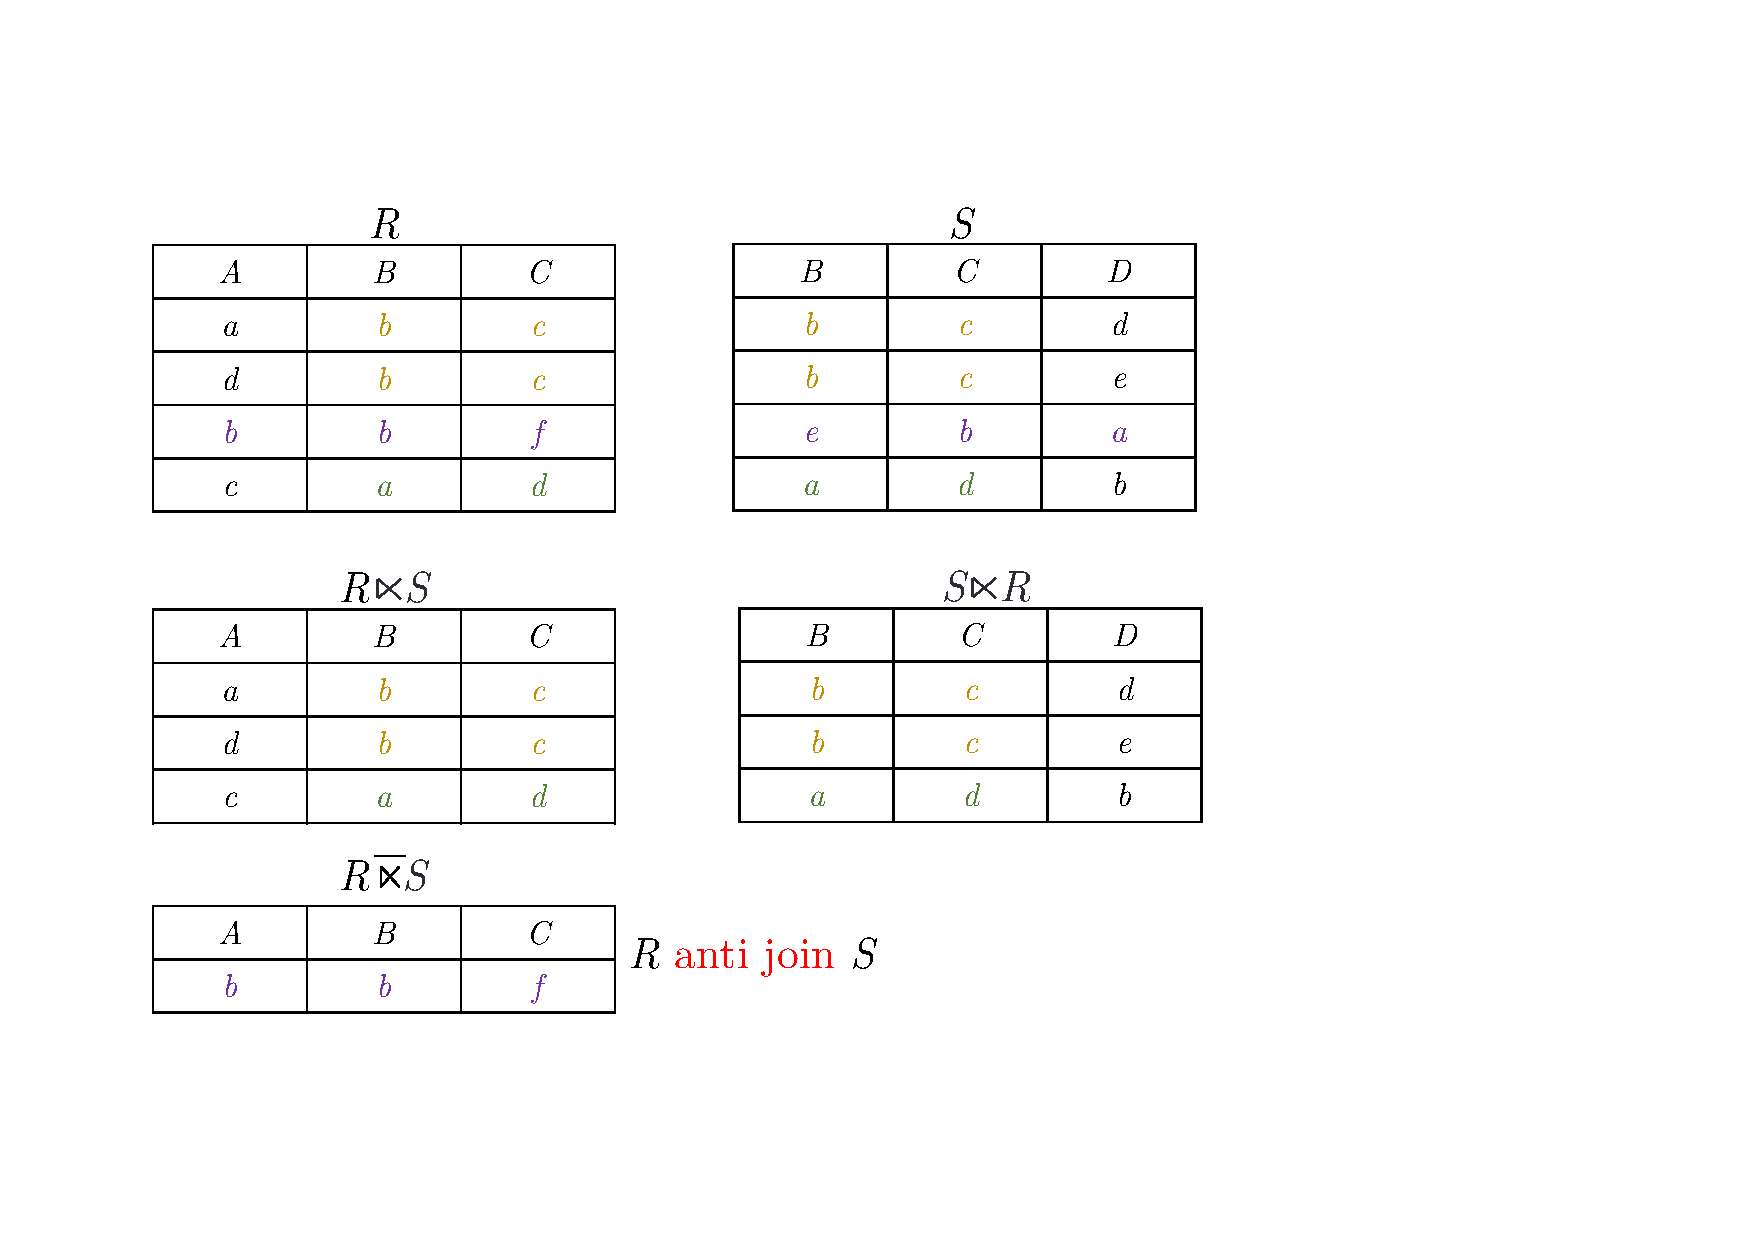
\includegraphics[width=.6\textwidth]{./figure/半连接.pdf}
    \caption{半连接示意图}
\end{figure}
 % FINISHED

\chapter{SQL}

\begin{introduction}[期末考试提纲]
  \item 了解数据类型、表的定义
  \item 掌握各种索引的定义及其作用
  \item 掌握各种查询表达操作的含义
  \item 能用SQL表达查询操作
  \item 表连接、分组聚集、集合、嵌套子查询、null、游标、with定义临时视图
\end{introduction}

SQL: Structured Query Languang

SQL语言的特点:
\begin{enumerate}
    \item 语言简洁,易学易用.
    \item 面向集合的操作方式,一次一集合.
    \item 高度非过程化.\textit{用户只需提出“做什么” ,无须告诉“怎么做”}
    \item 一体化.单一的结构——关系,带来了数据操作符的统一.
    \item 两种使用方式,统一的语法结构.
    \begin{enumerate}
        \item 既是自含式(用户使用)的
        \item 又是嵌入式的(程序员使用)
    \end{enumerate}
\end{enumerate}

\begin{table}[H]
  \centering
  \begin{tabular}{|c|c|}
    \hline
    \textbf{SQL功能} & \textbf{操作符} \\
    \hline
    数据定义 & \verb|create|, \verb|alter|, \verb|drop| \\
    \hline
    数据查询 & \verb|select| \\
    \hline
    数据修改 & \verb|insert|, \verb|update|, \verb|delete| \\
    \hline
    数据控制 & \verb|grant|, \verb|revoke| \\
    \hline
  \end{tabular}
  \caption{SQL主要操作符}
\end{table}

text2SQL: 建立自然语言与结构化数据之间的关系.

\section{数据定义}

\begin{figure}[H]
  \centering
  \begin{minipage}[t]{0.45\textwidth}
    \centering
    \includegraphics[width=\linewidth]{./figure/标准SQL.pdf}
    \caption{标准SQL中的数据定义对象}
  \end{minipage}
  \hfill
  \begin{minipage}[t]{0.5\textwidth}
    \centering
    \includegraphics[width=\textwidth]{./figure/实际.pdf}
    \caption{实际数据库(SQL Server)中的定义对象}
  \end{minipage}
\end{figure}

SQL Server: 模式把对象和用户分离开来.

对象命名: \verb|<数据库>.<模式>.<表>|.

\subsection{数据模式定义}

创建模式:
\begin{lstlisting}[language=SQL]
create schema <模式名>
create schema University.Library
\end{lstlisting}

数据库定义: SQL Server
\begin{lstlisting}[language=SQL]
create database <数据库名>
  [on [primary] <文件描述> <文件组> ...]
  [log on <文件描述> <文件组> ...]
\end{lstlisting}

最简单的创建数据库的命令: \verb|create databse University|.

\verb|use| 命令指定当前要使用的数据库: \verb|use University|.

\begin{lstlisting}[language=SQL]
create database demoDB1
on primary
( name = demo_dat1,
  filename = 'D:\SQL_Practice\demodata1.mdf',
  size = 10,
  maxsize = 50)
log on
(
  name = demo_log1,
  filename = 'D:\SQL_Practice\demodata1.ldf',
  size = 5,
  filegrowth = 5
)
\end{lstlisting}

数据库定义: MySQL
\begin{lstlisting}[language=SQL]
create database <数据库名>
  [ default character set utf8
    default collate utf8_Chinese_ci ]
\end{lstlisting}

\verb|create database| 等于 \verb|create schema|.

MySQL表空间:

\begin{figure}[H]
    \centering
    \includegraphics[width=.45\textwidth]{./figure/MySQL表空间.pdf}
    \caption{MySQL表空间}
\end{figure}

\begin{lstlisting}[language=SQL]
create tablespace myTs 'ts1.ibd' engine = innodb
create tablespace myTs add datafile
  'F:\\test_mysql_tablespace\\first.ibd'
create table myTb (...) tablespace myTs
\end{lstlisting}

创建基本表的语法命令:
\begin{lstlisting}[language=SQL]
create table <表名> (
  <列名> <数据类型> [default <缺省值>] [not null] [unique]
  [, <列名> <数据类型> [default <缺省值>] [not null] [unique]]
  ...
  [, primary key (<列名> [, <列名>] ...)]
  [, foreign key (<列名> [, <列名>] ...)
    references <表名> (<列名> [, <列名>] ...)]
  [, check(<条件>)]
)
\end{lstlisting}

下面是创建表的一些例子:
\begin{lstlisting}[language=SQL]
create table student
( sno char(8),
  sname char(8) not null default '佚名',
  age tinyint,
  sex char(1),
  primary key (sno),
  check (sex = 'M' or sex='F')
)
\end{lstlisting}

\begin{lstlisting}[language=SQL]
create table course
( cno char(8) primary key,
  cname char(8) not null unique,
  pcno char(8) foreign key references C(cno),
  credit tinyint
)
\end{lstlisting}

\begin{lstlisting}[language=SQL]
create table SC
( sno char(8) foreign key references S(sno),
  cno char(8) foreign key references C(cno),
  grade tinyint,
  primary key (sno, cno),
  check((grade is null) or grade between 0 and 100)
)
\end{lstlisting}

修改基本表: 更改、添加、除去列和约束.
\begin{lstlisting}[language=SQL]
alter table <表名>
  [add column <子句>]
  [add constraint <子句>]
  [drop <子句>]
  [alter column <子句>]
\end{lstlisting}

\begin{lstlisting}[language=SQL]
-- 在student表age列之后加入addr
alter table student add column addr CHAR(30) after age;
-- 把addr列重命名为address
alter table student change addr address CHAR(50) not null;
-- 试修改teacher表中的salary列的数据类型为bigint
alter table teacher modify salary bigint;
-- 重命名一个表中的列名从sal到salary
alter table rename sal to salary
\end{lstlisting}

删除基本表:
\begin{lstlisting}[language=SQL]
drop table <表名>;
\end{lstlisting}
删除表定义及该表的所有数据、索引、触发器、约束和权限规范.

drop table不能删除被foreign key约束所引用的表, 必须先除去foreign key约束或引用表.

任何引用已删除表的视图或存储过程必须通过drop view或drop procedure语句显式除去.

标准SQL中的信息视图:
\begin{lstlisting}[language=SQL]
INFORMATION_SCHEMA.SCHEMATA
INFORMATION_SCHEMA.TABLES
INFORMATION_SCHEMA.COLUMNS
INFORMATION_SCHEMA.CHECK_CONSTRAINTS
INFORMATION_SCHEMA.VIEWS
INFORMATION_SCHEMA.DOMAINS
\end{lstlisting}

MySQL中的信息视图查询:
\begin{lstlisting}[language=SQL]
select shcema_name from information_schema.schemata;
select table_name from information_schema.tables;
select column_name from information_schema.columns where table_name = 'student';
\end{lstlisting}

\begin{table}[H]
\centering
\label{tab:sysobjects}
\begin{tabular}{|l|l|l|}
\hline
\multicolumn{3}{|c|}{sysobjects} \\ \hline
\textbf{列名} & \textbf{数据类型} & \textbf{描述} \\ \hline
name & sysname & 对象名 \\ \hline
Id & int & 对象标识号 \\ \hline
xtype & char(2) & 对象类型 \\ \hline
uid & smallint & 所有者对象的用户ID \\ \hline
crdate & datetime & 对象的创建日期 \\ \hline
schema\_ver & int & 版本号,该版本号在每次表的架构更改时都增加 \\ \hline
\end{tabular}
\caption{表定义相关的字典表: SQL Server}
\end{table}

\begin{table}[H]
\centering
\label{tab:syscolumns}
\begin{tabular}{|l|l|l|}
\hline
\multicolumn{3}{|c|}{syscolumns} \\ \hline
\textbf{列名} & \textbf{数据类型} & \textbf{描述} \\ \hline
name & sysname & 列名或过程参数的名称 \\ \hline
id & int & 该列所属的表对象ID \\ \hline
 xtype & tinyint & systypes 中的物理存储类型 \\ \hline
xusertype & smallint & 扩展的用户定义数据类型ID \\ \hline
length & smallint & systypes 中的最大物理存储长度 \\ \hline
offset & smallint & 该列所在行的偏移量;如果为负,表示可变长度行 \\ \hline
type & tinyint & systypes 中的物理存储类型 \\ \hline
usertype & smallint & systypes 中的用户定义数据类型ID \\ \hline
isnullable & int & 表示该列是否允许空值 \\ \hline
\end{tabular}
\caption{表定义相关的字典表: SQL Server}
\end{table}

SQL中, 任何时候都可以执行一个数据定义语句, 随时修改数据库结构.

\subsection{数据类型}

\begin{table}[H]
\centering
\label{tab:mysql_int_types}
\begin{tabular}{|l|l|l|l|}
\hline
\textbf{数据类型} & \textbf{范围} & \textbf{unsigned范围} & \textbf{存储字节数} \\ \hline
tinyint & $-2^7 \sim 2^7 - 1$ & $0 \sim 2^8 - 1$ & 1字节 \\ \hline
smallint & $-2^{15} \sim 2^{15} - 1$ & $0 \sim 2^{16} - 1$ & 2字节 \\ \hline
mediumint & $-2^{23} \sim 2^{23} - 1$ & $0 \sim 2^{24} - 1$ & 3字节 \\ \hline
int & $-2^{31} \sim 2^{31} - 1$ & $0 \sim 2^{32} - 1$ & 4字节 \\ \hline
bigint & $-2^{63} \sim 2^{63} - 1$ & $0 \sim 2^{64} - 1$ & 8字节 \\ \hline
\end{tabular}
\caption{MySQL整数数据类型及其范围和存储字节数}
\end{table}

\begin{lstlisting}[language=SQL]
create table test_int (
  a(6) tinyint zerofill,
  b(6) tinyint unsigned );
insert into test_int values (1, 111);
select a, b from test_int;
-- a 000001 b 111
select a - b from test_int;
-- ERROR 1690 (22003): BIGINT UNSIGNED value is out of range
\end{lstlisting}

宽松模式: \verb|set sql_mode = 'ANSI'|. 对于违反数据约束的有一些默认操作.

严格模式: \verb|set sql_mode = 'traditional'|. 直接报错.


\begin{table}[H]
  \centering
  \begin{tabular}{|l|l|l|l|}
    \hline
    \textbf{数据类型} & \textbf{描述} & \textbf{unsigned范围} & \textbf{存储字节数} \\ \hline
    \verb|float|($m$, $d$) & \makecell[l]{单精度浮点数\\ $m$是总位数\\ $d$是小数点后位数} & ... & 4字节 \\ \hline
    \verb|double|($m$, $d$) & \makecell[l]{双精度浮点数\\ $m$是总位数\\ $d$是小数点后位数} & ... & 8字节 \\ \hline
    \makecell[l]{\texttt{decimal}($m$, $d$) \\ \texttt{numeric}} & \makecell[l]{精确小数\\ $m$是总位数\\ $d$是小数点后位数} & \makecell[l]{最大位数$m$为65 \\ 最大支持小数为$d$为30} & \\ \hline
    \verb|float|($n$) & ... & ... & \makecell[l]{$1\leq n \leq 24$是4字节\\ $25\leq n \leq 53$是8字节} \\ \hline
  \end{tabular}
  \caption{定点数与浮点数}
\end{table}

money使用4位小数存储数据, 容易发生小数的舍入错误.

\begin{table}[H]
  \centering
  \begin{tabular}{|l|l|l|l|}
    \hline
    \textbf{数据类型} & \textbf{范围} & \textbf{描述} & \textbf{存储字节数} \\ \hline
    \verb|char|($n$) & $0\sim 255$ & 定长字符串 & 4字节 \\ \hline
    \verb|varchar|($n$) & $0\sim 65,535$ & 变长字符串 & 实际字符串长度 \\ \hline
    \makecell[l]{\texttt{tinytext} \\ \texttt{text} \\ \texttt{mediumtext}\\ \texttt{longtext}} & \makecell[l]{$0\sim 2^8$\\ $0\sim 2^{16}$\\ $0\sim 2^{24}$ \\ $0\sim 2^{32}$} &  & \\ \hline
  \end{tabular}
  \caption{字符型}
\end{table}

\begin{lstlisting}[language=SQL]
-- 创建表时指定字符集和校对规则
CREATE TABLE users (
  name VARCHAR(100)
) CHARACTER SET utf8mb4 COLLATE utf8mb4_unicode_ci;
-- ci 表示不区分大小写

-- 查看服务器字符集
SHOW VARIABLES LIKE 'character_set%';
-- 查看数据库字符集
SHOW CREATE DATABASE mydb;
-- 查看表字符集
SHOW CREATE TABLE users;
\end{lstlisting}

\begin{table}[H]
    \centering
    \begin{tabular}{|l|l|p{5cm}|l|}
        \hline
        \textbf{类型名称} & \textbf{日期格式} & \textbf{日期范围} & \textbf{存储需求} \\ \hline
        year & YYYY & 1901 $\sim$ 2155 & 1 个字节 \\ \hline
        time & HH:MM:SS & -838:59:59 $\sim$ 838:59:59 & 3 个字节 \\ \hline
        date & YYYY-MM-DD & 1000-01-01 $\sim$ 9999-12-31 & 3 个字节 \\ \hline
        datetime & YYYY-MM-DD HH:MM:SS & 1000-01-01 00:00:00 $\sim$ 9999-12-31 23:59:59 & 8 个字节 \\ \hline
        timestamp & YYYY-MM-DD HH:MM:SS & 1980-01-01 00:00:01 UTC $\sim$ 2040-01-19 03:14:07 UTC & 4 个字节 \\ \hline
    \end{tabular}
    \caption{日期类型及其描述}
    \label{tab:date_types}
\end{table}

\begin{table}[H]
  \centering
  \begin{tabular}{|l|l|}
    \hline
    \textbf{数据类型} & \textbf{描述} \\ \hline
    \verb|enum('v1', 'v2', ...)| & 只能取一个值 \\ \hline
    \verb|set('v1', 'v2', ...)| & 可以取多个值 \\ \hline
  \end{tabular}
  \caption{枚举型}
\end{table}

\begin{lstlisting}[language=SQL]
create table test_enum(
  a enum('男' ,'女'),
  b set('1', '2', '3', '4') )
insert into test_enum values ('男', '2,4')
\end{lstlisting}

\begin{table}[H]
  \centering
  \begin{tabular}{|l|l|}
    \hline
    \textbf{数据类型} & \textbf{大小} \\ \hline
    \verb|binary(n)| & 255 \\ \hline
    \verb|varbinary(n)| & 16384 \\ \hline
    \verb|tinyblob, blob, mediumblob, longblob| & 256, 16K, 16M, 4G \\ \hline
  \end{tabular}
  \caption{二进制类型}
\end{table}

下面是几个关于数据类型的问题:
\begin{enumerate}
    \item char 还是 varchar?
    \begin{table}[H]
      \centering
      \begin{tabular}{|l|l|l|}
        \hline
        \textbf{特性} & \textbf{CHAR} & \textbf{VARCHAR} \\ \hline
        存储方式 &	固定长度 & 可变长度 \\ \hline
        存储效率 & 可能浪费空间(固定长度填充空格) &	高效(仅存储实际数据 + 长度信息)\\ \hline
        检索速度 & 更快(直接定位)& 稍慢(需计算长度) \\ \hline
        适用场景 & 固定长度数据(如代码、哈希值) &	可变长度数据(如姓名、地址) \\ \hline
        空格处理 & 自动填充空格(需注意业务逻辑) &	不填充空格 \\ \hline
      \end{tabular}
    \end{table}
    \item 显式数据类型转换: 
    \begin{lstlisting}[language=SQL]
cast ( 表达式 as 数据类型 [(数据长度)] )
convert ( 数据类型 [(数据长度)], 表达式 [, 输出样式] )
select cast( 123.45 as decimal(10,4) )            -- 输出结果: 123.4500
select cast( 123.45 as decimal(10,1) )            -- 输出结果: 123.5
select cast( 12.34567 as money )                  -- 输出结果: 12.3457
select 'My age is: ' + cast( 28 as char(4) )      -- 输出结果: My age is: 28
select cast( cast( 123.45 as int ) as char(10) )  -- 输出结果: 123
select convert( varchar(30), getdate(), 106 )     -- 输出结果: 17 08 2012
select convert( varchar(30), getdate(), 110 )     -- 输出结果: 08-17-2012
select cast( 'SQL' as binary(3) )                 -- 输出结果: 0x53514C
    \end{lstlisting}
    \item 隐式数据类型转换: 执行\verb|select 1 + '1'|, 结果会是2; 执行\verb|select 1 + 'a'|, 会显示类型转换错误.
    \item 特殊类型: XML, JSON, Array, 空间数据.
    \item 用户定义数据类型UDDT(User-defined Datatype).
    \begin{itemize}
      \item 标准SQL: \verb|create domain 域名 数据类型|;
      \item SQL Server: \verb|create type phone_number from varchar(20) not null|.
      \item Oracle: 
      \begin{lstlisting}[language=SQL]
create type animal_ty as OBJECT(
  breed varchar2(25),
  name vharchar2(25),
  birthday date
)
      \end{lstlisting}
    \end{itemize}
    \item 冗长主码的危害: 占据很大的表空间; 减少索引项, 增加了磁盘I/O数, 减慢索引速度.
\end{enumerate}

MySQL中的自增字段:
\begin{lstlisting}[language=SQL]
create table test_incr(
  id bigint auto_increment,
  name char(10)
)
\end{lstlisting}

SQL Server中的序列号: identity.
\begin{lstlisting}[language=SQL]
create table customer(
  cust_id smallint identity(100, 20) not null,
  -- identity 有一个起始数和增量值
  cust_name varchar(50) not null
)
\end{lstlisting}

SQL Server中的序列号: sequence.
\begin{lstlisting}[language=SQL]
create sequence mySeq as int start with 1 increment by 1
insert into myTb(id, Name) values (next value for mySeq, 'Tom')
insert into myTb(id, Name) values (next value for mySeq, 'jerry')
\end{lstlisting}

uniqueidentifier 产生跨数据库和服务器的全局唯一标识符(GUID), newid()函数产生uniqueidentifier 类型的值, newsequentialid()产生的GUID总是大于先前通过该函数生成的GUID.

如果表中有一列被声明为rowversion, 只要行被修改, 其rowversion
列就会发生改变. 它是跨表唯一的, 任何表的修改都会使该值递增.

\subsection{索引}

\begin{definition}[索引]
  索引是数据库管理系统中用于加速数据检索的核心工具. 
  它通过创建特定数据结构(如B树、哈希表等), 
  将数据表中的某些列的值与对应的物理存储位置关联起来, 从而大幅提升查询效率.
\end{definition}

索引的作用:
\begin{itemize}
  \item 加速查询;
  \item 支持排序和分组;
  \item 保证唯一性;
  \item 优化连接操作.
\end{itemize}

\begin{lstlisting}[language=SQL]
create [unique] index 索引名
  [using { btree | hash }]
on 表名 (列名 [asc/desc] [, 列名asc/desc] ...)

drop index 索引名
\end{lstlisting}

\begin{figure}[H]
  \centering
  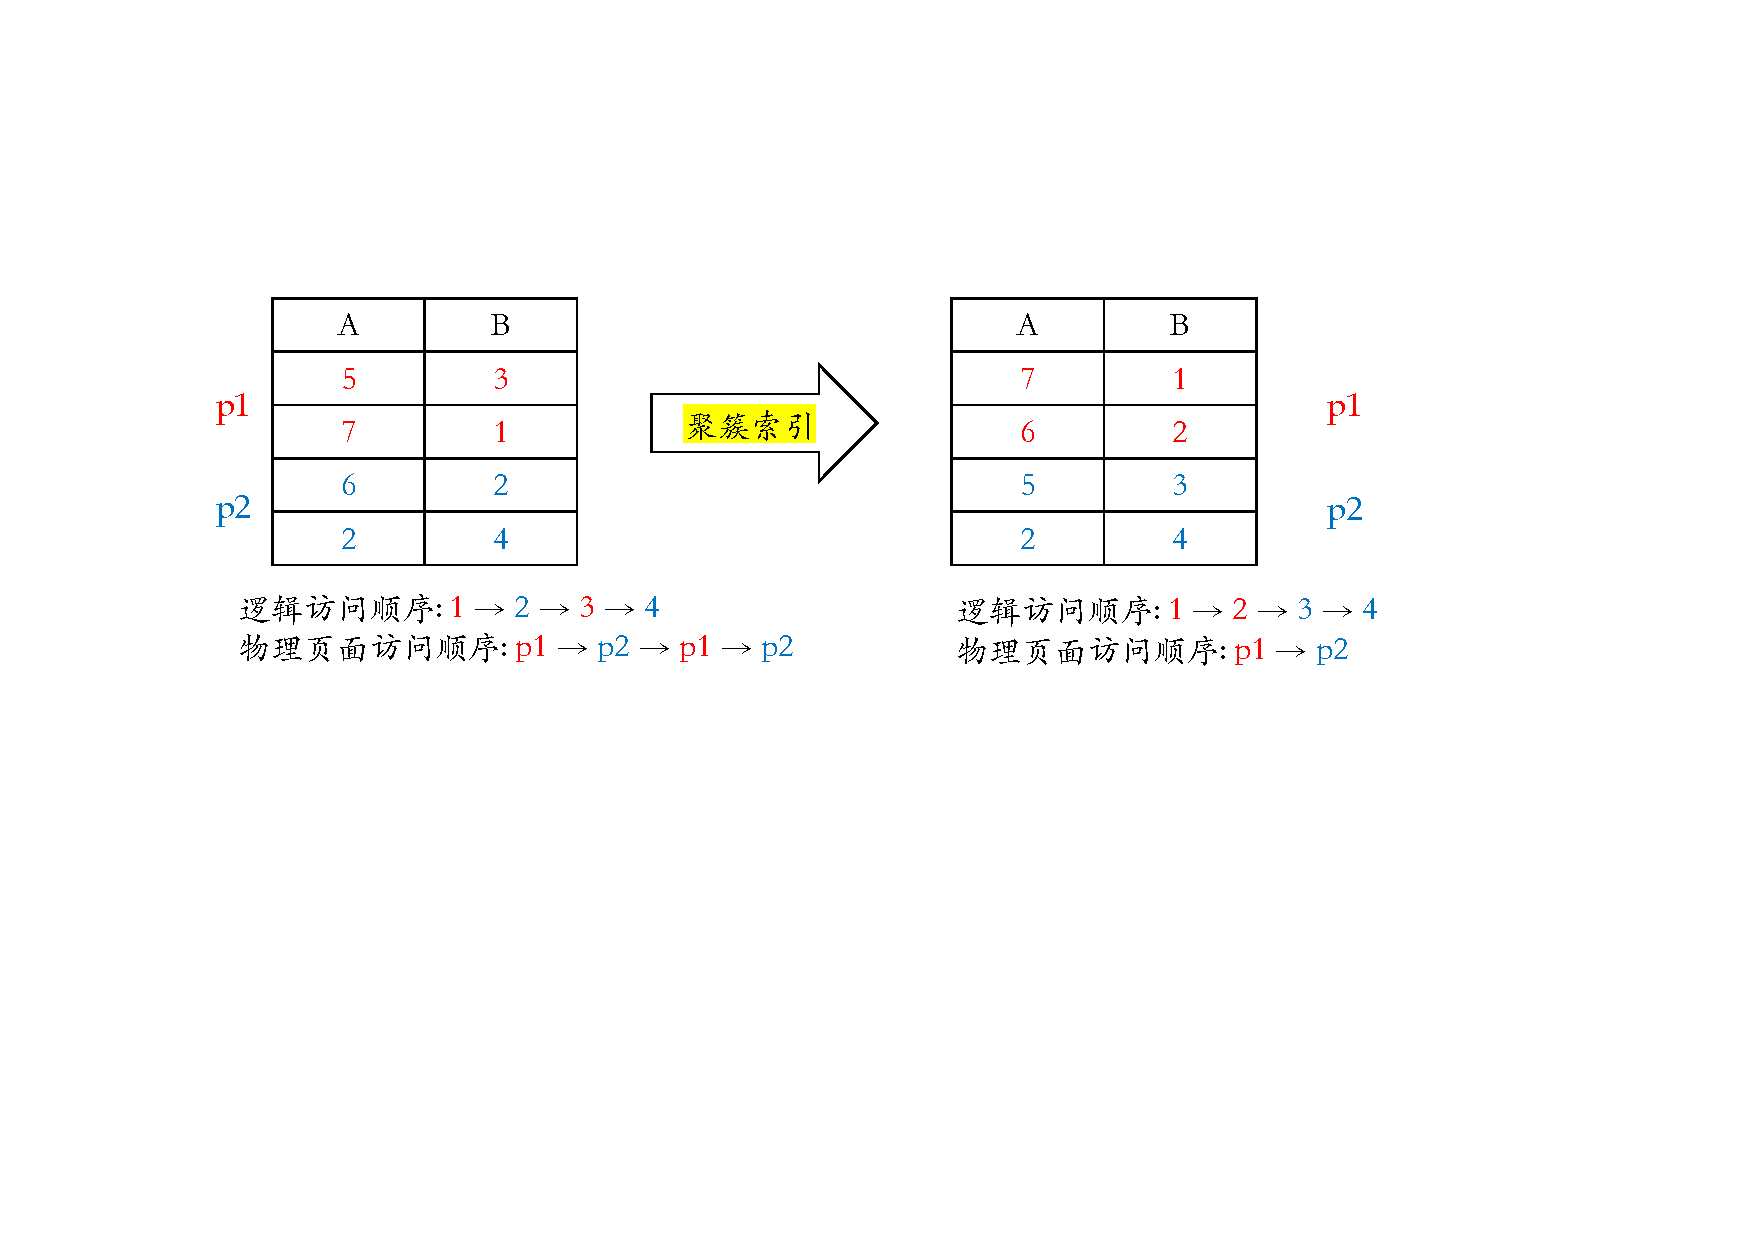
\includegraphics[width=.8\textwidth]{figure/聚簇索引.pdf}
  \caption{聚簇索引}
  \label{fig:cluster}
\end{figure}

\begin{definition}[索引碎片]
  索引碎片: 页面逻辑顺序与物理顺序不一致.
\end{definition}

\textbf{下面是若干实现索引的方法:}
\begin{itemize}
  \item 聚簇索引(cluster): 表中元组按索引项的值排序并物理地聚簇在一起. \textcolor{red}{聚簇索引使得逻辑访问顺序和物理存储顺序尽可能一致.} 如图\ref{fig:cluster}.
  \item 组合索引: 建立在多个属性列上的索引. 
  
  索引 (A, B, C) 的B+树会先按 A 排序, 再在 A 相同的情况下按 B 排序, 最后在 B 相同的情况下按 C 排序.

  必须满足\textbf{最左前缀原则}: 即查询条件必须从索引的最左列开始连续匹配.

  假如我们针对索引(user\_id, name) 的查询:
  \begin{lstlisting}[language=SQL]
SELECT user_id, name FROM users WHERE user_id = 100;
  \end{lstlisting}
  那么可以\textit{直接从索引获取数据, 无需访问表数据.}

  但是查询\verb|SELECT * FROM users WHERE user_id = 100;|需\textbf{回表}查询所有列.
\end{itemize}

\textbf{下面是描述索引的性质:}
\begin{itemize}
  \item 覆盖索引: 覆盖索引的核心是“索引覆盖查询需求”. 当查询的字段全部被索引包含时, 数据库可以直接从索引中获取结果, 而不需要回表查询数据行.
  \begin{lstlisting}[language=SQL]
create index my_idx on R(A) include B
  \end{lstlisting}
  换言之, 这是在描述一个索引\verb|my_idx|会覆盖对B的查询!
  \item 过滤索引: 在索引的定义中加入where语句, 索引中只包括那些满足过滤条件的列值.
  \begin{lstlisting}[language=SQL]
create index filter_idx1 on R(A) where A is not null
  \end{lstlisting}
  应用: 比如大部分男而少部分女, 可只对女做索引. 这些是低频值, 不用每次都会更新索引结构.
  \item 函数索引: 
  \begin{lstlisting}[language=SQL]
select * from student where UPPER(name) = 'TOM'
create index idx2 on student(UPPER(name))
-- 由于建立了一个针对 UPPER(name) 的索引, 会就是把 UPPER(name) 来查
  \end{lstlisting}
\end{itemize}

\textbf{索引的使用说明:}
\begin{itemize}
  \item 一个表上可建多个索引;
  \item 可以动态地定义索引;
  \item 随时建立和删除索引;
  \item 索引可以提高\textcolor{red}{查询效率};
  \item 耗费空间;
  \item 降低插入、删除、更新效率.
\end{itemize}

\begin{definition}[索引选择度]
  索引选择度 = 1 / 索引列的唯一值个数.\footnote{这里老师的定义有点怪. 根据\hyperlink{https://www.red-gate.com/simple-talk/databases/sql-server/performance-sql-server/14-sql-server-indexing-questions-you-were-too-shy-to-ask/}{14 SQL Server Indexing Questions You Were Too Shy To Ask}: The ratio of unique values within a key column is referred to as index selectivity. The more unique the values, the higher the selectivity, which means that a unique index has the highest possible selectivity. The query engine loves highly selective key columns, especially if those columns are referenced in the WHERE clause of your frequently run queries. The higher the selectivity, the faster the query engine can reduce the size of the result set. The flipside, of course, is that a column with relatively few unique values is seldom a good candidate to be indexed.
  
  这里的定义是: NUM\_DISTINCT / NUM\_ROWS. 在这种情况下, 选择度高的更好.}

  在这种情况下, 应该选择索引选择度低的建立索引.
\end{definition}

\begin{definition}[索引过滤性]
  索引过滤性=查询结果行数/总行数.

  现在我们假设每个都分布均匀, 比如基数为NUM\_DISTINCT, 每个里面的记录=个数都一样.
  \begin{itemize}
    \item "="的索引过滤性为 1/NUM\_DISTINCT.
    \item "$\neq$"的索引过滤性为 (NUM\_DISTINCT-1)/NUM\_DISTINCT.
    \item "$\geq$"的索引过滤性为 更大的/NUM\_DISTINCT.
  \end{itemize}
\end{definition}

\begin{example}
  我们假设SC分布在10个页中, 平均每个学生选修3门课, 每门课程有3个学生选.

  有下面的三个操作:
  \begin{itemize}
    \item Q1: 查询某个学生所修的课程 (with probability $p_1$);
    \item Q2: 查询选修某门课程的学生 (with probability $p_2$);
    \item I: 插入选课元组 (with probability $1-p_1-p_2$).
  \end{itemize}
  求问: 当前最好应该使用怎样的索引?
\end{example}

\textit{ 解答. }
\begin{table}[ht]
\centering
\begin{tabular}{lcccc}
\hline
操作 & 无索引 & sno 索引 & cno 索引 & 全索引 \\
\hline
Q1 & 10 & 4 & 10 & 4 \\
Q2 & 10 & 10 & 4 & 4 \\
I & 2 & 4 & 4 & 6 \\
\hline
代价 & $2 + 8p_1 + 8p_2$ & $4 + 6p_2$ & $4 + 6p_1$ & $6 - 2p_1 - 2p_2$ \\
代价最小时概率分布 & $p_1 = p_2 = 0.1$ & $p_1 = 0.5, p_2 = 0.1$ & $p_1 = 0.1, p_2 = 0.5$ & $p_1 = p_2 = 0.4$ \\
\hline
\end{tabular}
\caption{不同索引下的操作代价与最优概率分布}
\end{table}

为什么是4? 因为访问索引一次+返回的三个元组3次.

\subsection{视图定义}

\begin{definition}[视图]
  视图是命名的、从基本表中导出的虚表, 它在物理上并不存在, 存在的只是其定义, 属于外模式.

  视图中的数据是从基本表中导出的, 每次对视图查询都要重新计算.

  视图之上可以再定义视图.
\end{definition}

\begin{lstlisting}[language=SQL]
create view view_name[(列名[,列名] ...)]
  as (查询表达式)
[with check option]

drop view view_name
\end{lstlisting}

\begin{lstlisting}[language=SQL]
create view computer_teacher
as
  ( select tno, tname, salary
    from department, teacher
    where department.tno = teacher.tno
    and dname = '计算机系')

select  tname
from    computer_teacher
where   salary > 1000
\end{lstlisting}

视图的优点:
\begin{itemize}
  \item 使不同用户可以从不同角度观察同一数据;
  \item 逻辑独立性: 视图作为基本表与外模式之间的映象;
  \item 安全性: 限制用户数据的访问范围;
\end{itemize}

\begin{theorem}[不可更新的视图: 不含基表主码]
  视图定义中不包括基表主码时, 视图不可更新.
\end{theorem}

\begin{proof}
  设当前的视图定义为$V(A_1,A_2,...,A_m)$, 这其中不含基表$R$的主键$P$. 那么当我们视图对视图更新时, 这个更新操作会变成对基表的更新. 唯一的问题在于: 主键$P$自动的被填充为null, 而这种插入操作显然是不合法的, 因而此时视图不可更新.
\end{proof}

\begin{theorem}[不可更新的视图: 包含聚集函数]
  视图定义中包含聚集函数时, 视图不可更新.
\end{theorem}

\begin{proof}
  原因在于: 对于聚集值的更新无法回逆到基表上.
\end{proof}

\begin{theorem}[不可更新的视图: 不含连接属性]
  视图定义中没有包括连接属性时, 视图不可更新.
\end{theorem}

\begin{lstlisting}[language=SQL]
create table RT (A int , B int);
create table ST (B int , C int);
insert into RT values (1,2),(2,3);
insert into ST values (1,2),(2,3);

create view joinV as
(select A, C
 from RT, ST
 where RT.B = ST.B)
\end{lstlisting}

现在试图: \verb|insert into joinV values (3, 3)|.

\begin{figure}[H]
    \centering
    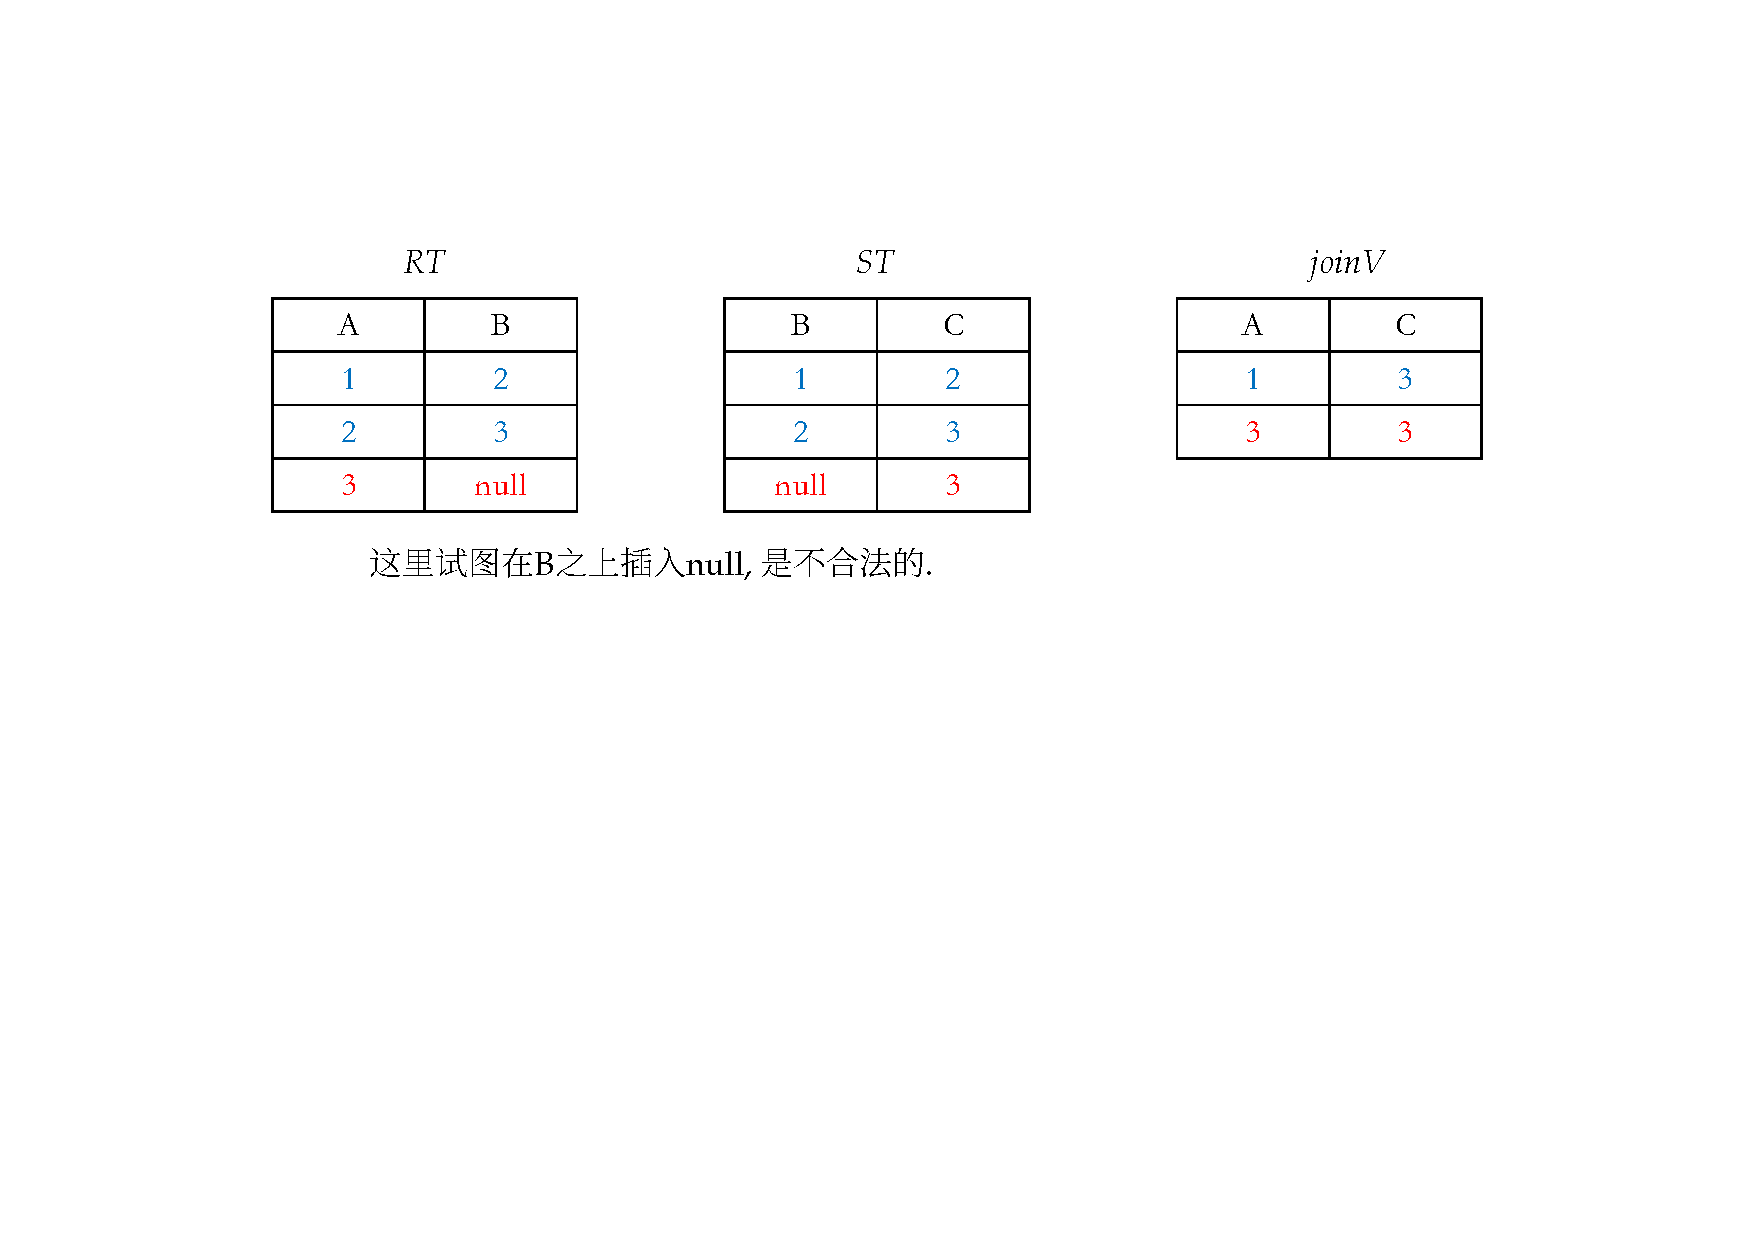
\includegraphics[width=.8\textwidth]{figure/不合法的视图更新.pdf}
    \caption{不可更新的视图: 不含连接属性}
\end{figure}

不可更新视图还包括:
\begin{itemize}
  \item select子句中的目标列包含了聚集函数;
  \item select子句中使用unique或distinct关键字;
  \item select子句中包含经算术表达式计算出来的列;
  \item from子句中包含了多个表;
  \item 包含了group by子句.
\end{itemize}

这些都是因为违反了\textbf{全关系系统准则 6: 视图更新准则}. 要存在一个算法可以无二
义地把更新要求转换为对基本表的更新序列.

\subsection{临时表和内存表}

\begin{table}[H]
\centering
\begin{tabular}{|l|l|l|}
\hline
 & 临时表 & 内存表 \\
\hline
存储 & 表结构和数据都存储在内存中 & 表结构存储在磁盘中,表数据存储在内存中 \\
\hline
会话 & 单个会话独享 & 多个会话共享 \\
\hline
断开连接 & 表结构和表数据都没了 & 表结构和表数据都存在 \\
\hline
服务重启 & 表结构和表数据都没了 & 表结构存在,表数据不存在 \\
\hline
\end{tabular}
\caption{临时表与内存表的比较}
\end{table}

\subsection{公用表表达式CTE}

\begin{lstlisting}[language=SQL]
with S-total (sno, value) as
      select sno, sum (grade)
      from SC
      group by sno
    S-total-avg(value) as
      select avg (value)
      from S-total
select sno
from S-total, S-total-avg
where S-total.value >= S-total-avg.value
\end{lstlisting}

\begin{lstlisting}[language=SQL]
values row(1,2,3), row(10,9,8)
union all
values row(-1,-2,0),row(10,29,30),row(100,20,-9)
\end{lstlisting}

\subsection{分区表}

\begin{definition}[分区表]
  把逻辑上统一的数据分割成较小的、可以独立管理的物理单元(分片)进行存储.
\end{definition}

分区表的优点:
\begin{itemize}
  \item 增强可用性;
  \item 维护方便;
  \item 均衡I/O;
  \item 改善查询性能.
\end{itemize}

一般的分区方式:
\begin{itemize}
  \item 范围分区: 根据某个属性值的范围进行分区;
  \item 散列分区: 通过分区编号将数据均匀散列到I/O设备上, 使得这些分区大小一致;
  \item 复合分区: 先使用范围分区; 再在每个分区内使用散列分区.
\end{itemize}

\section{数据查询}

开门见山: 数据查询只需要会下面的语法即可.
\begin{lstlisting}[language=SQL]
Select     <目标列>
From       <数据源表>
Where      <行过滤>
Group by   <分组>
Having     <分组过滤>
Union      <合并>
Order by   <输出排序>
Limit      <输出行数>
\end{lstlisting}

数据查询必须要经过: 笛卡尔积 $\to$ 选择 $\to$ 投影.

\begin{figure}[H]
    \centering
    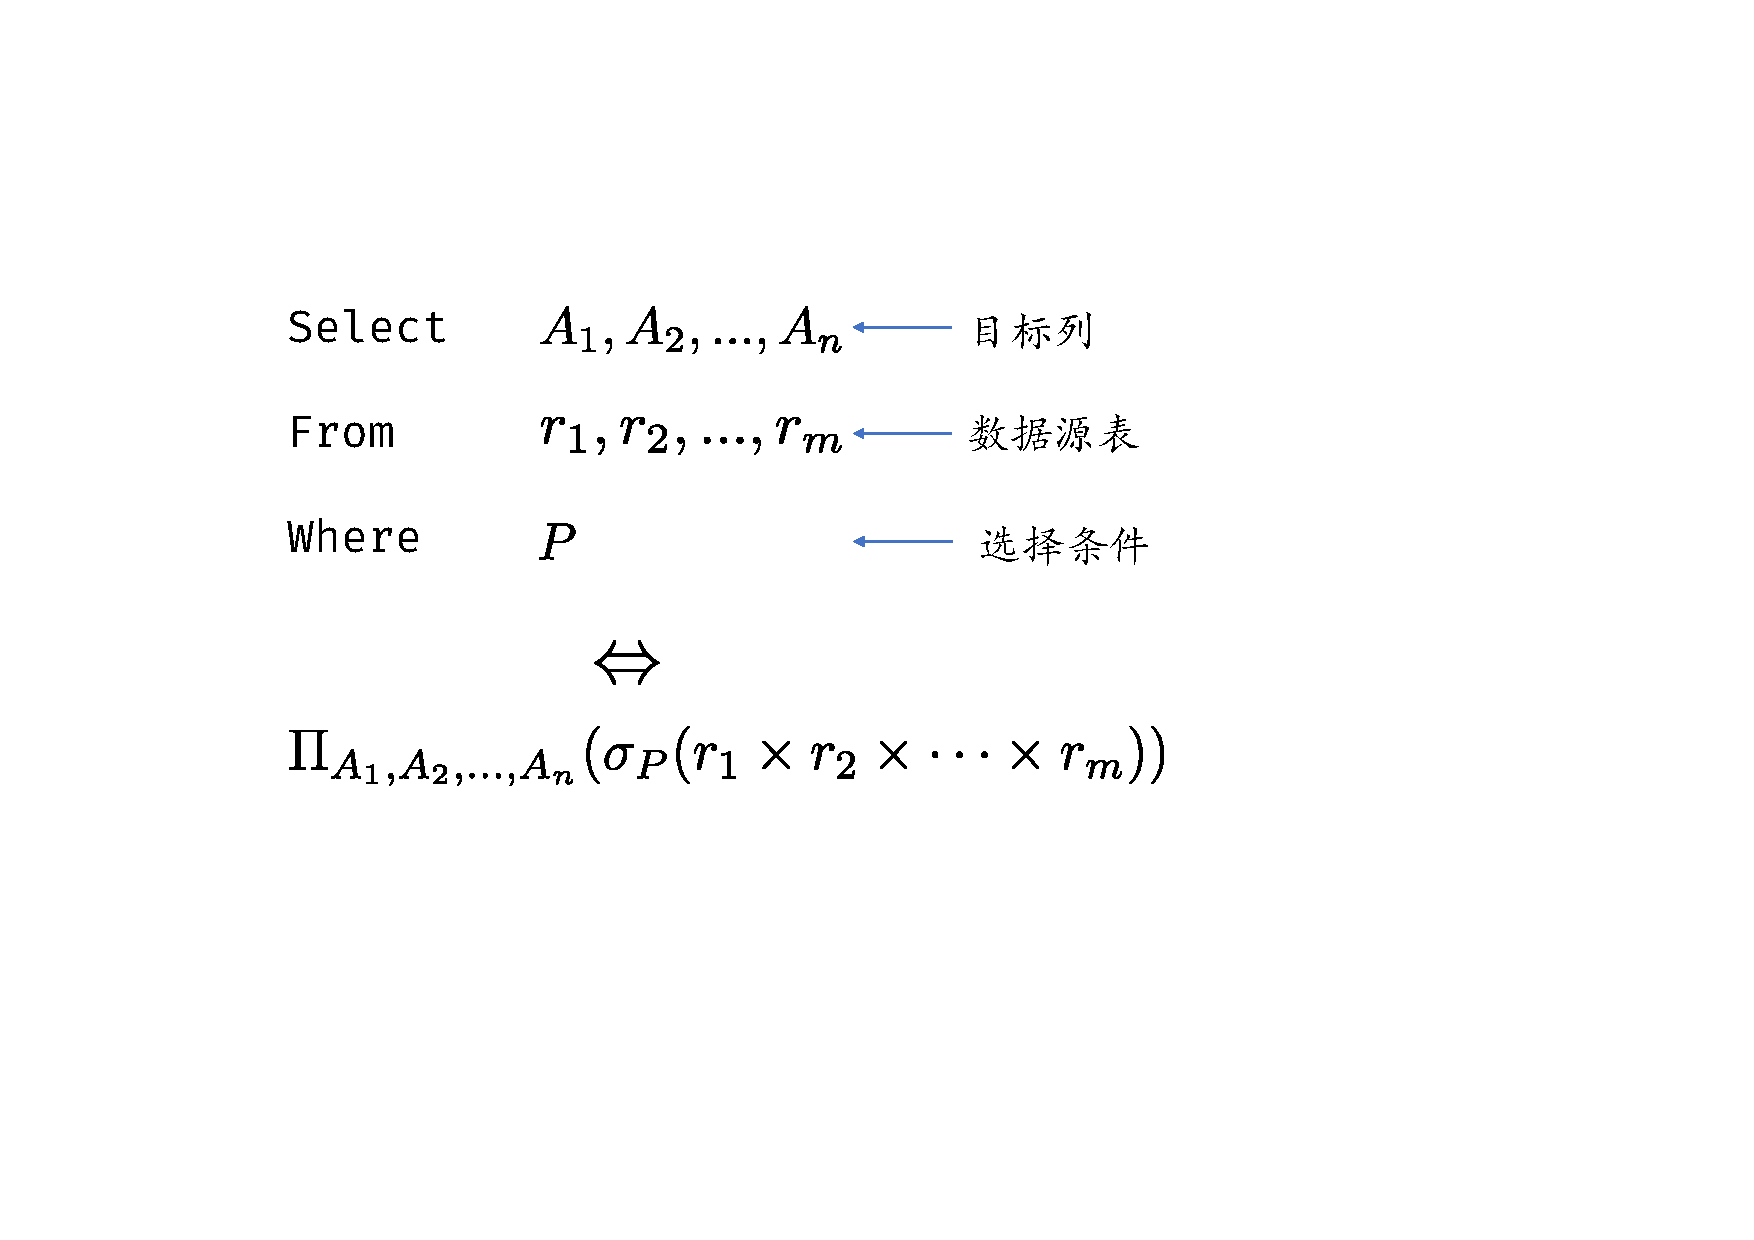
\includegraphics[width=.5\textwidth]{figure/数据查询.pdf}
    \caption{SQL查询基本结构}
\end{figure}

\begin{example}
  找出选修课程的学生姓名、课程名、成绩.
\end{example}

\textit{ 解答. }最基础的解是:
\begin{align*}
    \Pi_{sname,cname,grade} (S \bowtie SC \bowtie C).
\end{align*}
可以写成上面的三步走的形式, 如下图:
\begin{figure}[H]
    \centering
    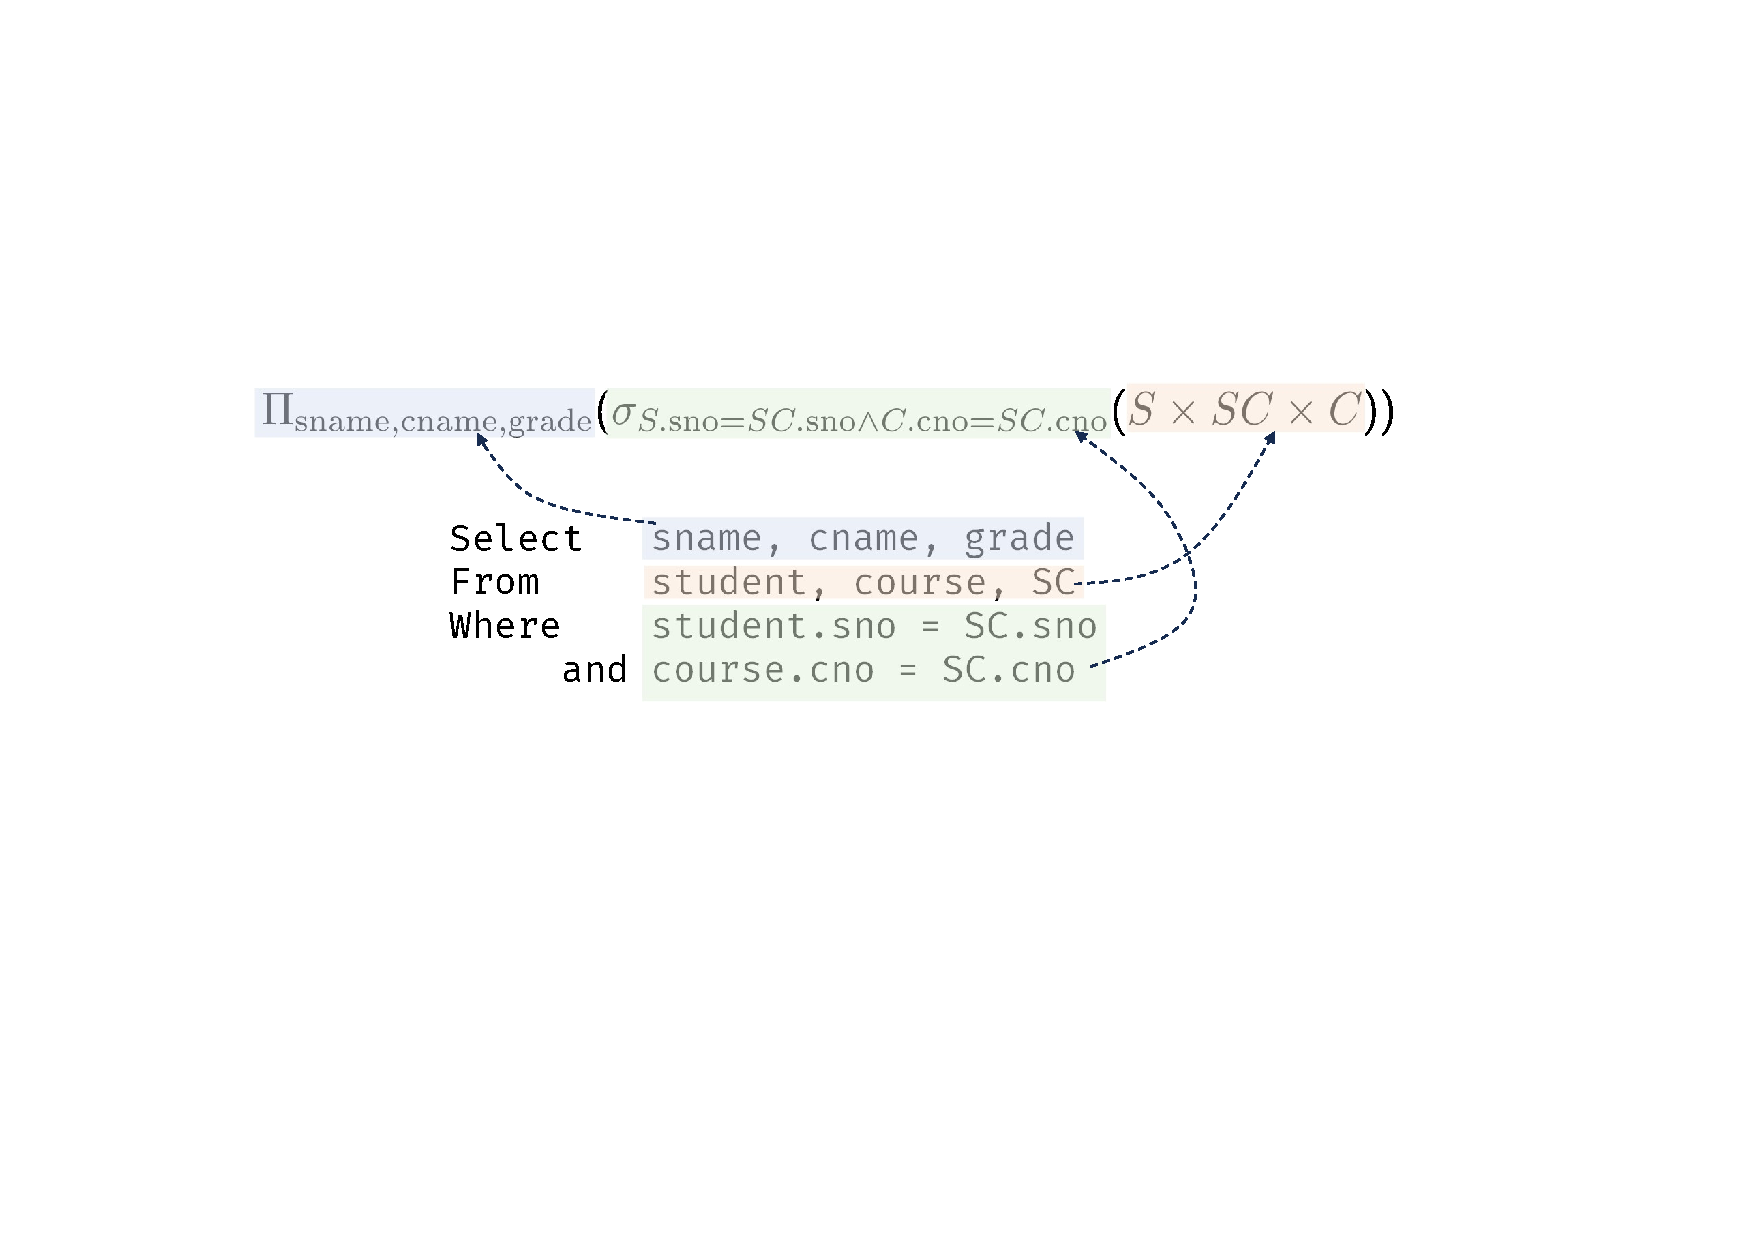
\includegraphics[width=.7\textwidth]{figure/查询例题1.pdf}
    \caption{数据查询三步走}
\end{figure}

\begin{example}
  写出与\textcolor{red}{$R(A,B) \bowtie S(B,C)$}等价的SQL.
\end{example}

\textit{ 解答. }
\begin{lstlisting}[language=SQL]
Select  A, R.B, C
From    R, S
Where   R.B = S.B
\end{lstlisting}

\begin{example}
  寻找每个学生在哪个系.
\end{example}

\textit{ 解答. }
\begin{lstlisting}[language=SQL]
Select     sname, dname
From       student, department
Where      dname = '计算机系'
      and  student.dno = department.dno
\end{lstlisting}

\begin{lstlisting}[language=SQL]
-- 给出所有学生的所有信息
select *
from student

-- 给出所有学生的姓名及出生日期
select sname, 2025-age
from student

-- 给出每个老师信息的自然语言描述
select  tname + '老师的工资是' + salary
        + ',年龄是' + age
        + ',职称是' + title
from teacher

-- 列出成绩在60~80之间的学生学号
-- 优化小窍门: 使用 between 合并两个比较谓词
select sno
from SC
where grade between 60 and 80
\end{lstlisting}

!!!注意, SQL缺省为保留重复值, 也可以用关键字 \textcolor{red}{\texttt{all}} 显式指明; 若要去掉重复行, 可以用关键字 \textcolor{red}{\texttt{distinct}} 指明.
\begin{align*}
    \Pi_A(R) = \texttt{select distinct }A\texttt{ from }R
\end{align*}

优化小窍门: 只在必要时使用 \textcolor{red}{\texttt{distinct}}.

输出顺序: \texttt{order by 列名 [asc | desc]}.
\begin{lstlisting}[language=SQL]
select *
from student
order by age asc, sname desc
-- 按照年龄升序输出学生信息, 相同年龄按照姓名降序

select tname, salary*2
from teacher
order by 2
-- 按照 输出列 的编号排序

select sname
from student
order by age
-- 排序列可以不是 输出列
\end{lstlisting}

更名运算: 可以出现在 \verb|select| 和 \verb|from| 子句中. \verb|old_name (as) new_name|.

\begin{lstlisting}[language=SQL]
select  sname '姓名',
        sex '性别',
        2025 - age '出生日期'
from student
order by 出生日期
-- 或者 order by 3

select S2.sno
from SC as S1, SC as S2
where S1.sno = 's1'
  and S1.cno = 'c1'
  and S2.cno = 'c1'
  and S1.grade < S2.grade
-- 找出比 s1 学生选修 c1 课程成绩高的学生号
\end{lstlisting}

\subsection{空值}

数据库中允许取null, 就变成了三值逻辑. true, false, unknown.
\begin{itemize}
  \item A-Mark null: 表示“未知的”. 值存在, 只是当前没有获得该信息.
  \item T-Mark null: 表示“不适用”.
\end{itemize}

\textcolor{red}{全关系系统准则 3: 空值的系统化处理. 全关系型DBMS应支持空值概念, 并用系统化的方式处理空值.}

注意: 运算中牵扯到了null, 结果都是null, 例如: \verb|null <> null| 结果为null.

注意: 空值测试. \verb|is [not] null|.
\begin{itemize}
  \item 除 \verb|is [not] null| 之外, 空值不满足任何查找条件.
  \item 如果null参与算术运算, 则该算术表达式的值为null.
  \item 如果null参与比较运算, 则结果可视为unknown.
\end{itemize}

\begin{lstlisting}[language=SQL]
select sno
from SC
where grade is null
-- 不要写成 where grade = null
\end{lstlisting}

MySQL中的空值处理函数:
\begin{itemize}
  \item \verb|isnull(expr)|: 如果 \verb|expr| 值为空, 返回1, 否则为0;
  \item \verb|ifnull(check_expr, replace_value)|: 如果 \verb|check_expr| 值为空, 返回\verb|replace_value|; 否则返回 \verb|check_expr|.
  \item \verb|nullif(expr1, expr2)|: 如果两个表达式相等则返回空值, 否则返回第一个表达式.
  \item \verb|coalesce(expr1, expr2, ... )|: 返回第一个不为null的\verb|expr|.
\end{itemize}

\begin{lstlisting}[language=SQL]
select sno, cno, ifnull (grade, 0)
from SC

select sno, cno, coalesce (grade, 0)
from SC
where coalesce (grade, 0) < 60
\end{lstlisting}

当指定 \verb|order by| 的时候, \verb|asc| 首先输出空值, \verb|desc| 最后输出空值.

如果要求首先输出空值, 然后由大到小输出非空值怎么办?
\begin{lstlisting}[language=SQL]
select  id, val,
        1 - isnull(val) as is_null
from order_null
order by is_null, val desc
\end{lstlisting}

\subsection{连接运算}

连接类型:
\begin{itemize}
  \item \verb|inner join|.
  \item \verb|left out join|.
  \item \verb|right out join|.
  \item \verb|full out join|.
\end{itemize}

\begin{lstlisting}[language=SQL, caption={不用外连接表达查询的例子}]
-- 列出所有老师的教工号、姓名、工资、所教课程号
select tno, tname, salary, cno
from teacher, TC
where teacher.tno = TC.tno
unoinselect tno, tname, salary, null
from teacher
where tno not in (select tno from TC)
\end{lstlisting}

\begin{lstlisting}[language=SQL, caption={用外连接表达查询的例子}]
-- 列出所有老师的教工号、姓名、工资、所教课程号
select tno, tname, salary, cno
from teacher left join TC
      on teacher.tno = TC.tno
\end{lstlisting}

inner join: 只保留符合连接条件的元组.
\begin{figure}[H]
    \centering
    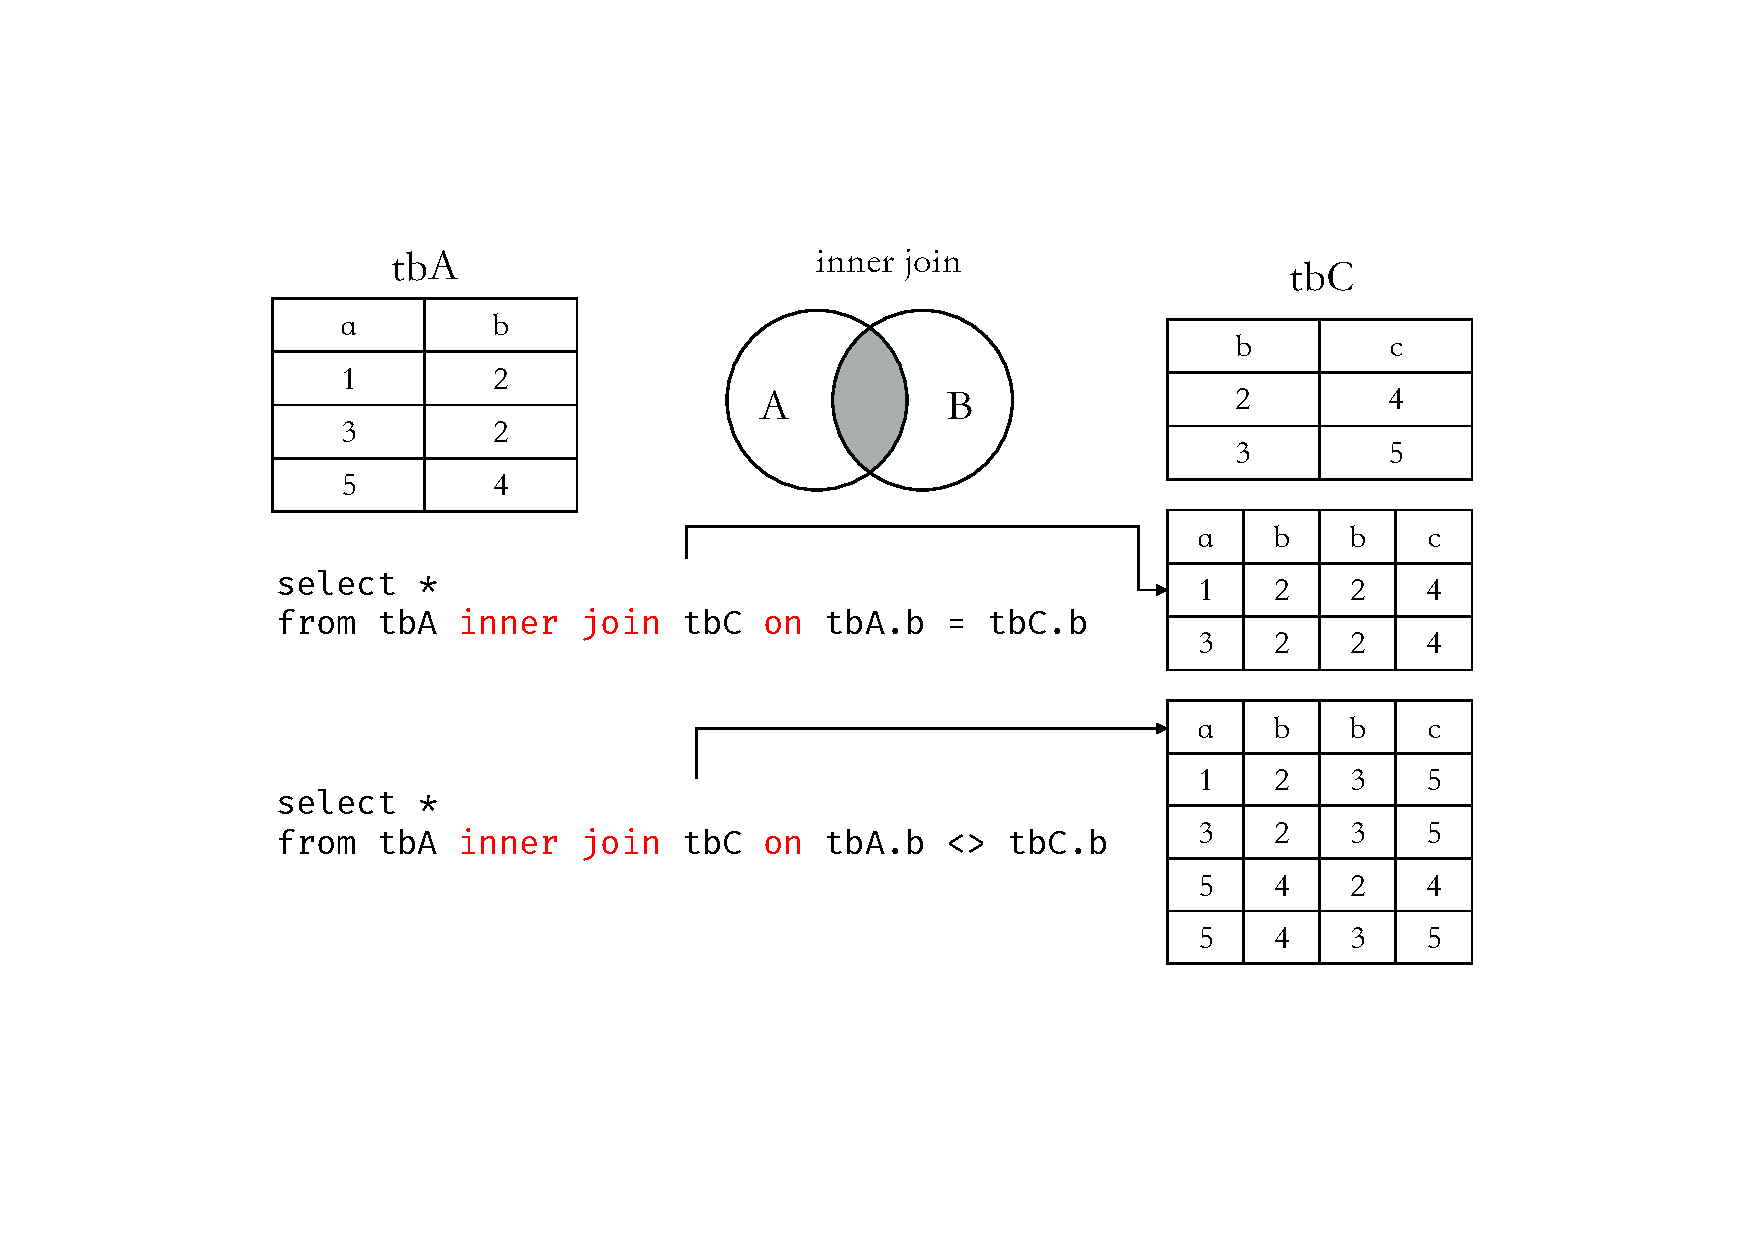
\includegraphics[width=.55\textwidth]{figure/inner_join.pdf}
    \caption{inner join示例}
\end{figure}

left join: 对于失配部分, 保留左边信息+null.

\begin{figure}[H]
    \centering
    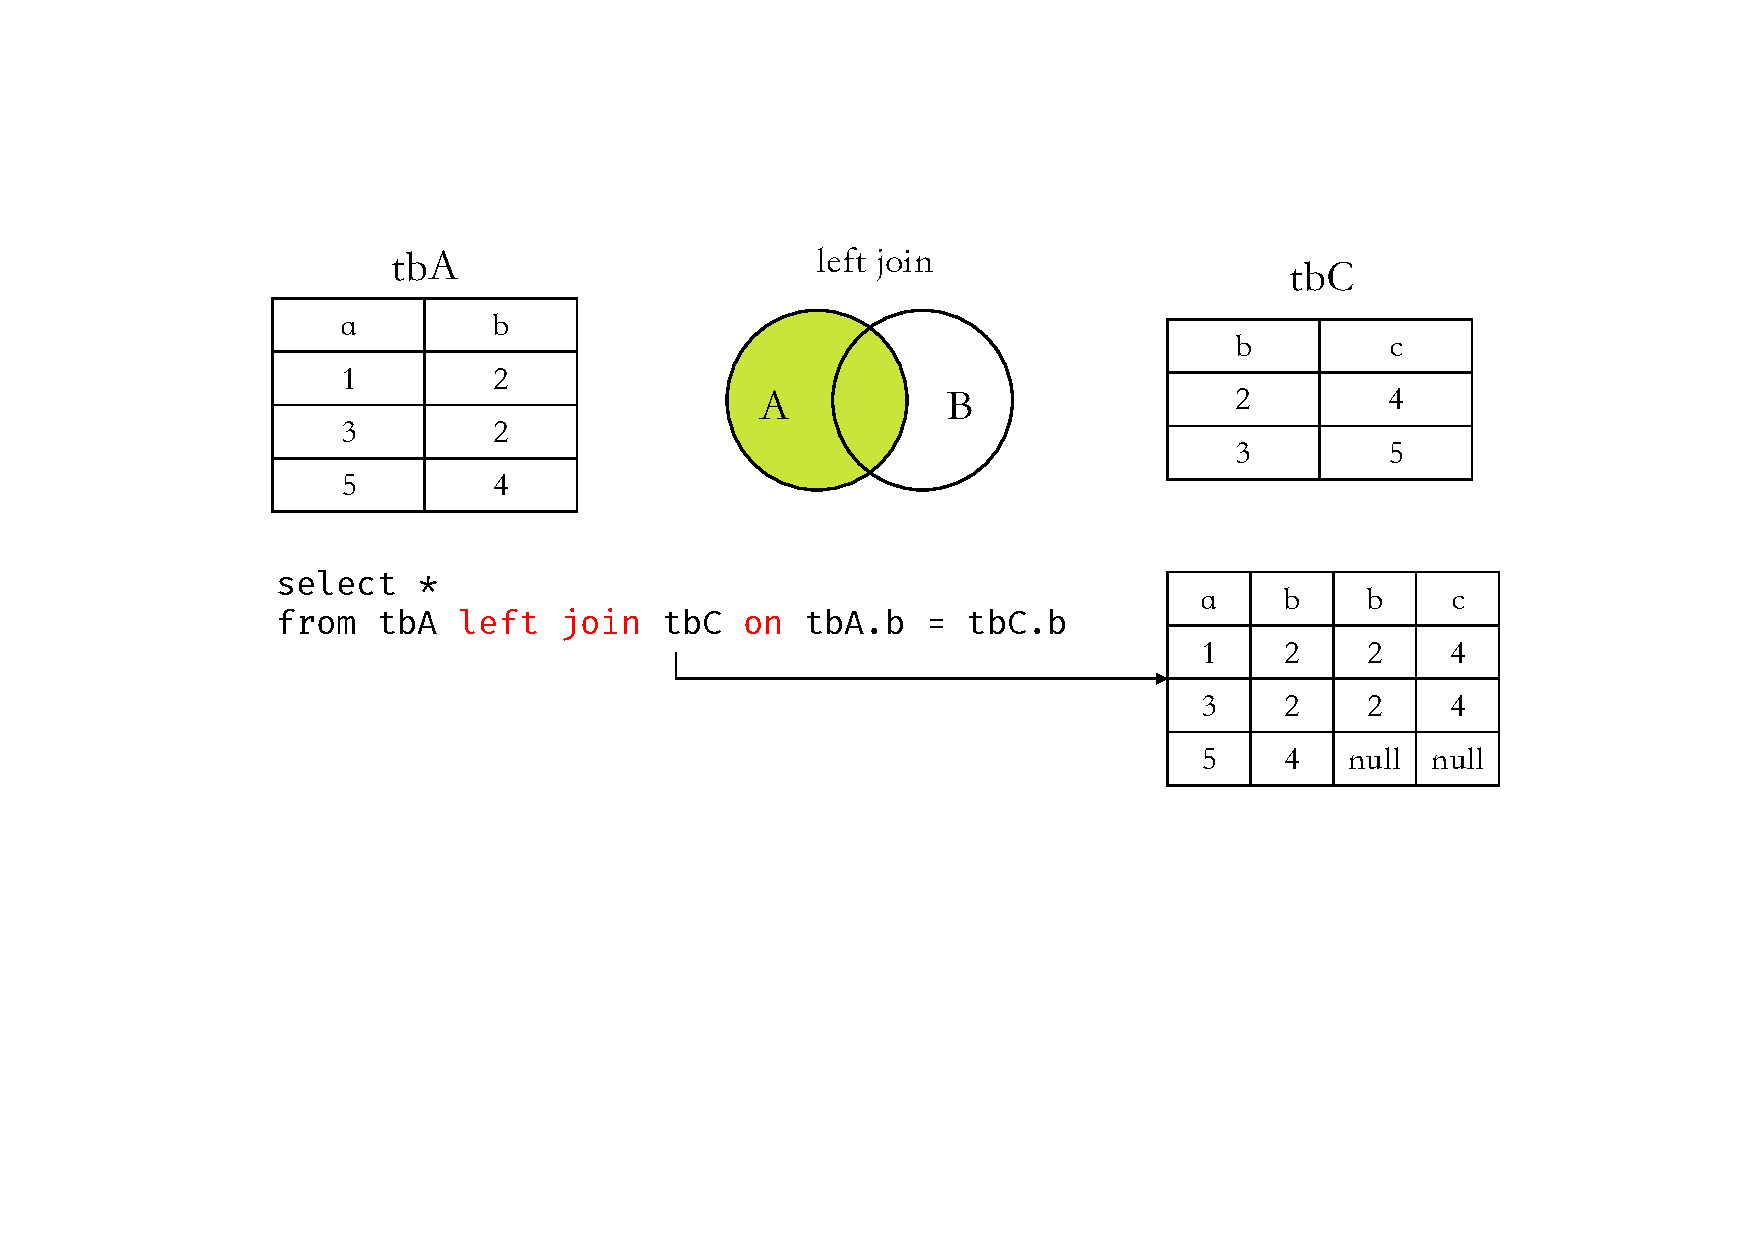
\includegraphics[width=.55\textwidth]{figure/left_join.pdf}
    \caption{left join示例}
\end{figure}

right join: 对于失配部分, 保留右边信息+(左边)null.

\begin{figure}[H]
    \centering
    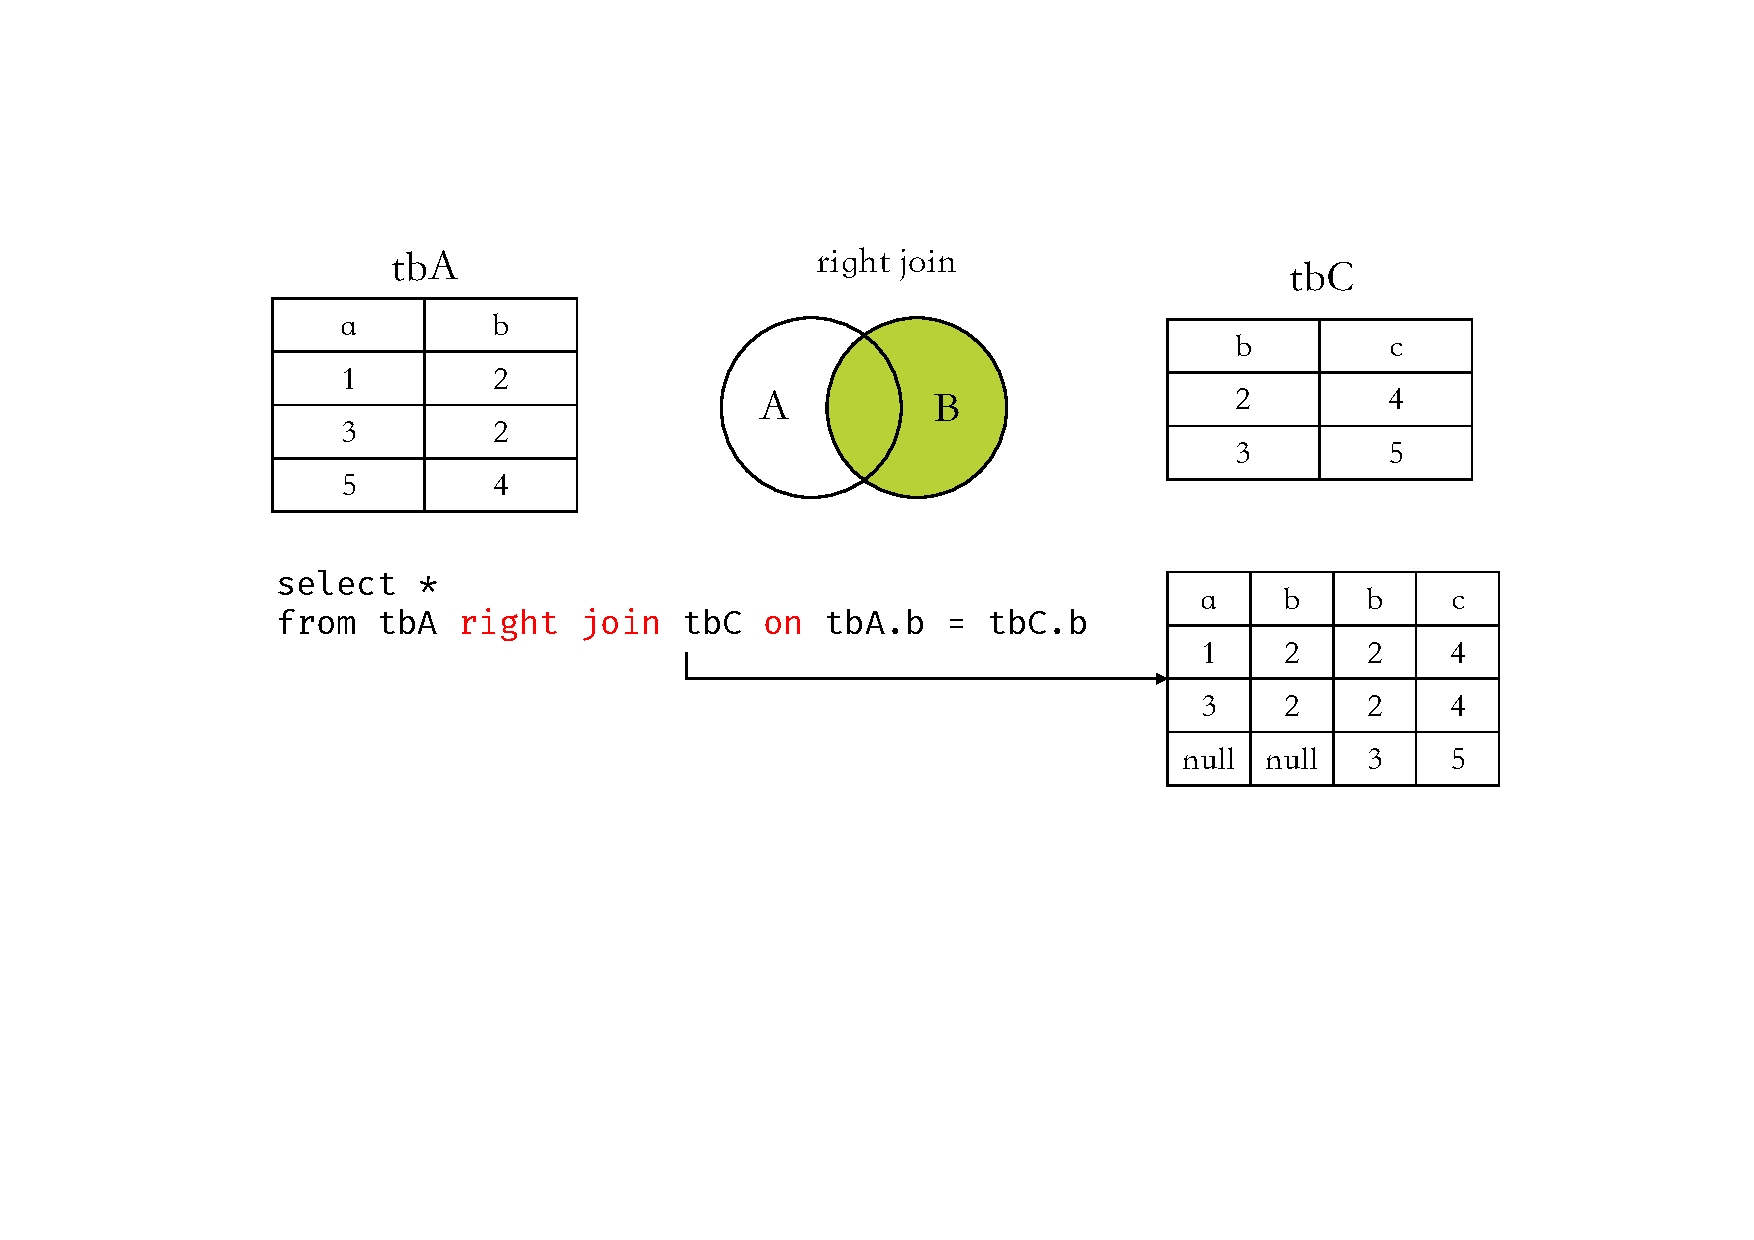
\includegraphics[width=.55\textwidth]{figure/right_join.pdf}
    \caption{right join示例}
\end{figure}

left join excluding inner join: 保留左边表中和右边失配的部分.

\begin{figure}[H]
    \centering
    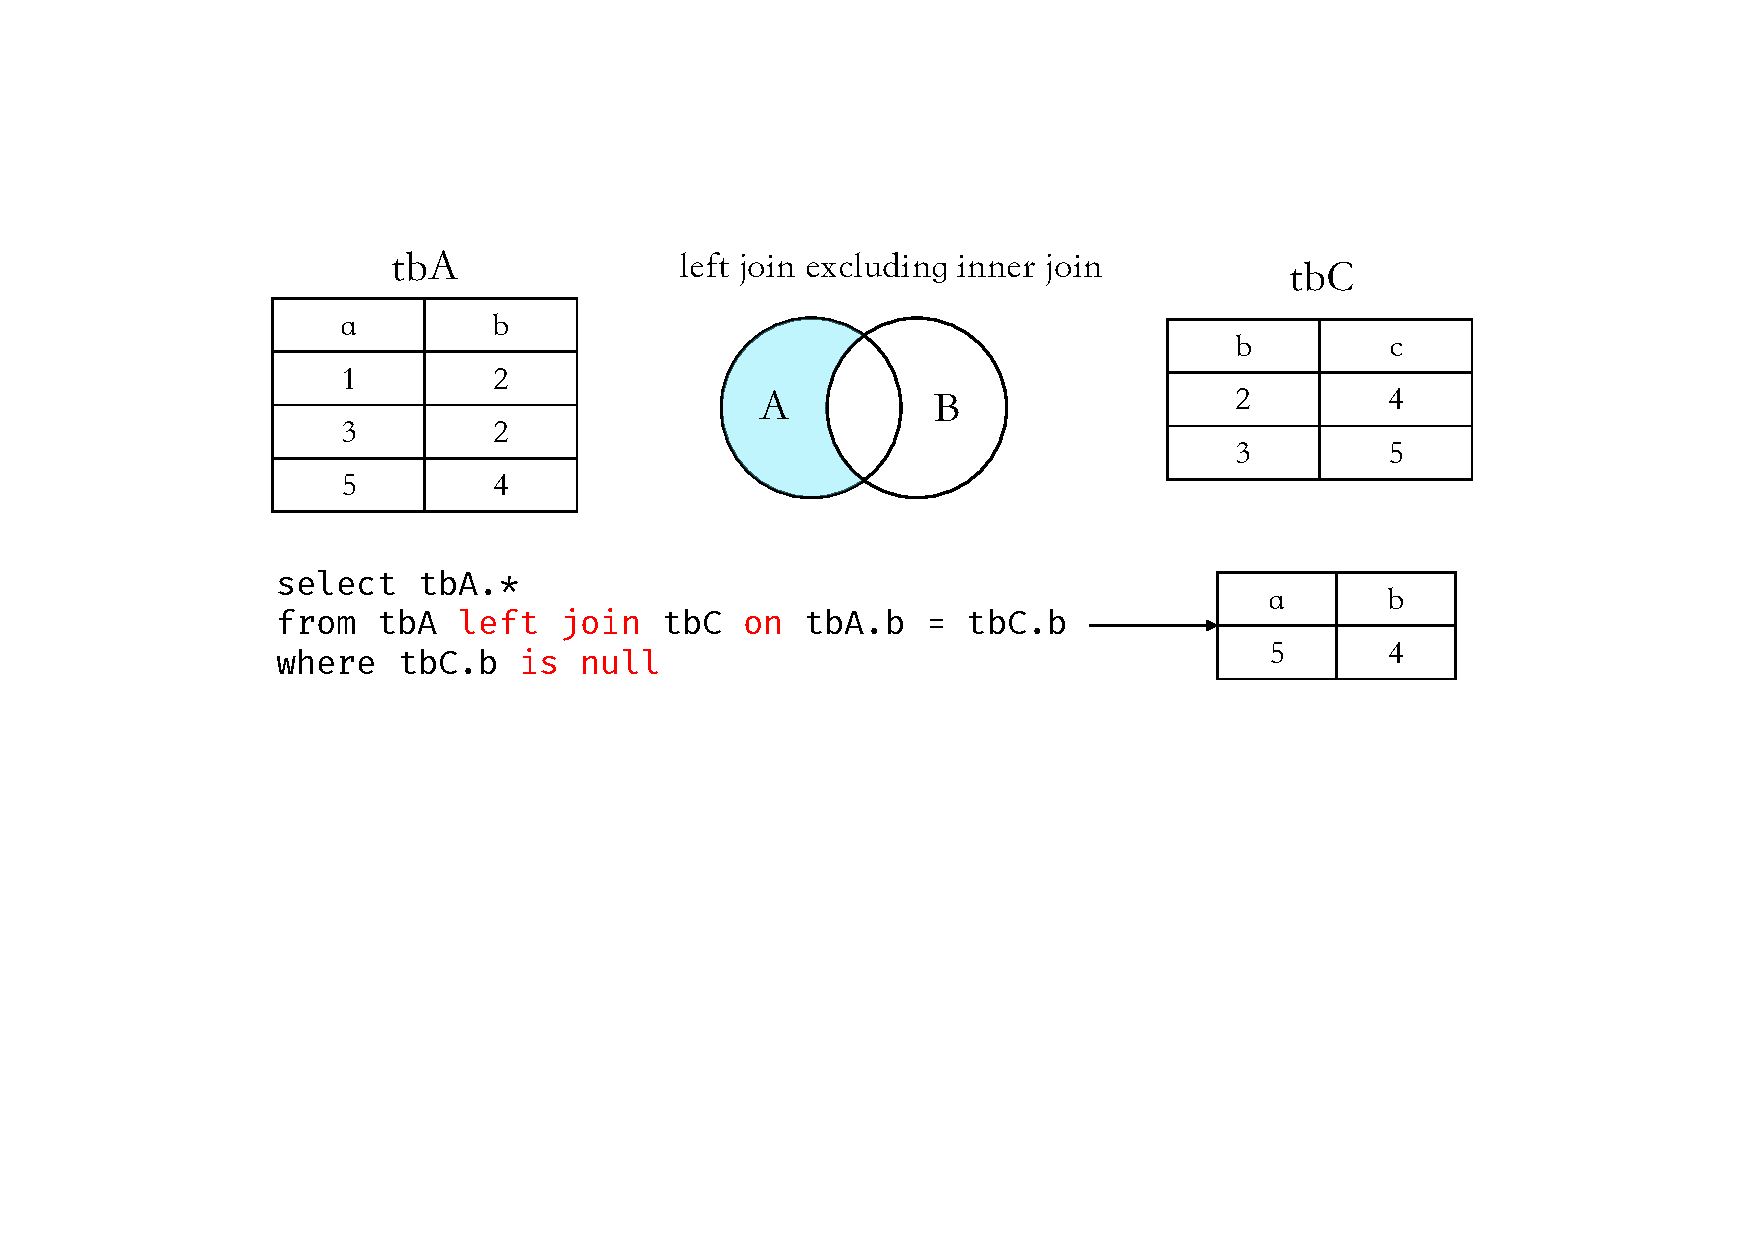
\includegraphics[width=.55\textwidth]{figure/left_join_ex_inner_join.pdf}
    \caption{left join excluding inner join}
\end{figure}

full join excluding inner join: 分别保留两边失配的部分.

\begin{figure}[H]
    \centering
    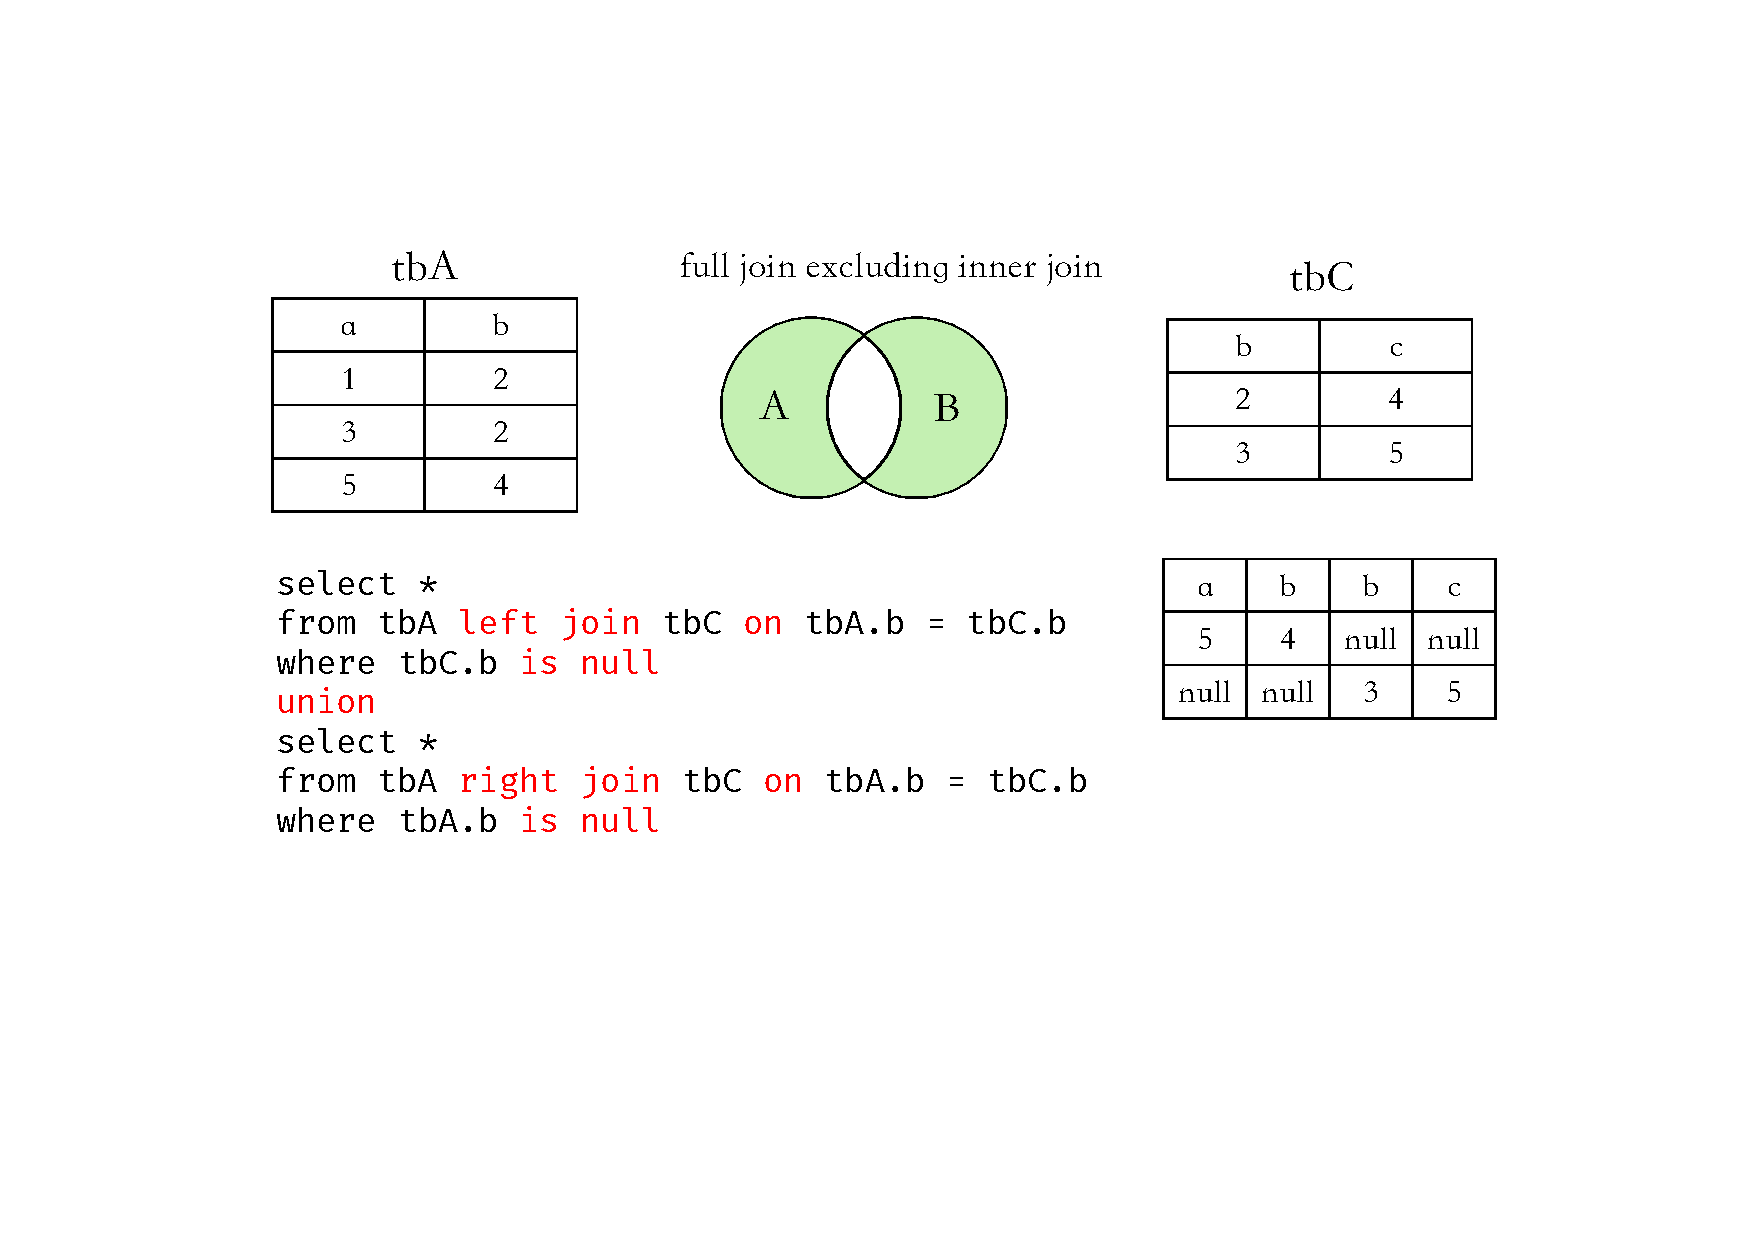
\includegraphics[width=.55\textwidth]{figure/full_join_ex.pdf}
    \caption{full join excluding inner join}
\end{figure}

cross join: \verb|(R cross join S) as T|: 两个关系的笛卡尔积.

\begin{figure}[H]
    \centering
    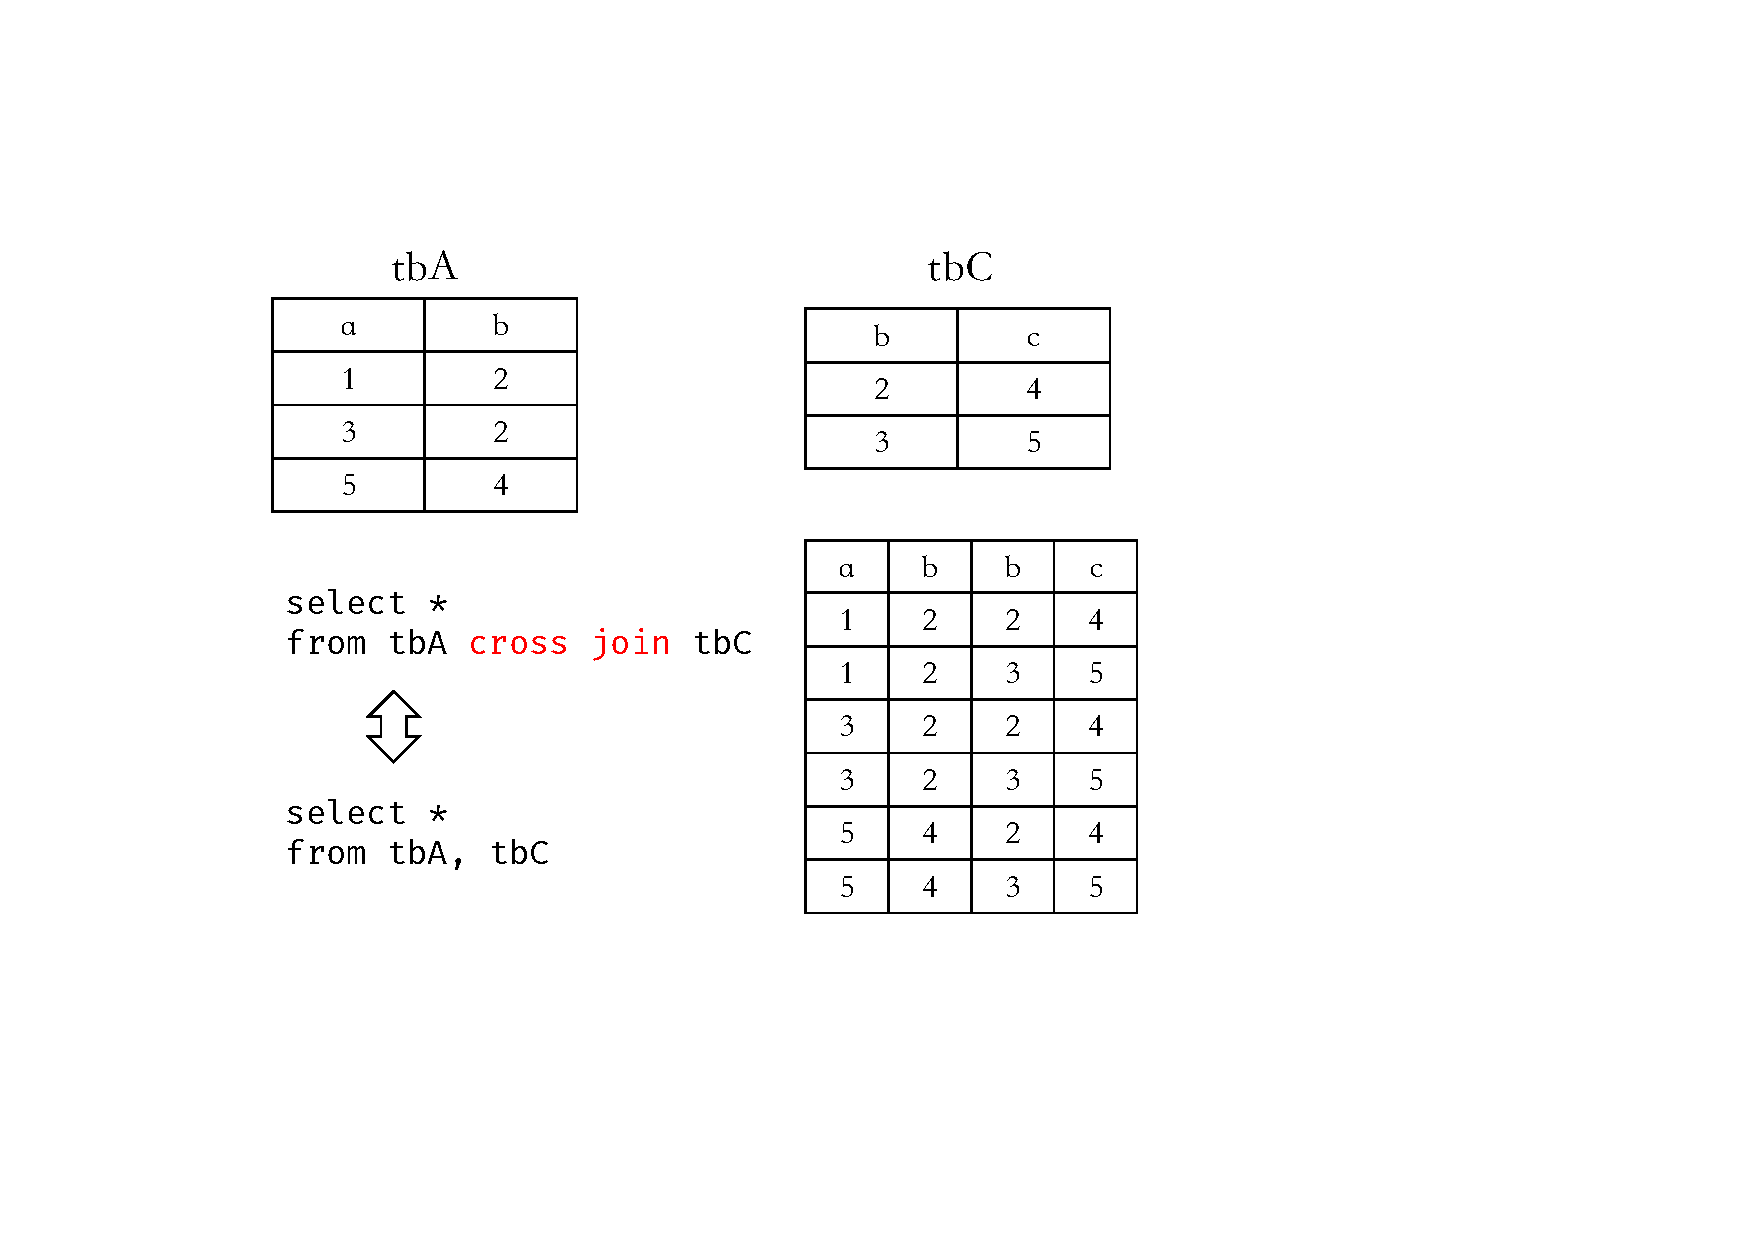
\includegraphics[width=.5\textwidth]{figure/cross_join.pdf}
    \caption{cross join}
\end{figure}

natural join: 匹配相同部分.

\begin{figure}[H]
    \centering
    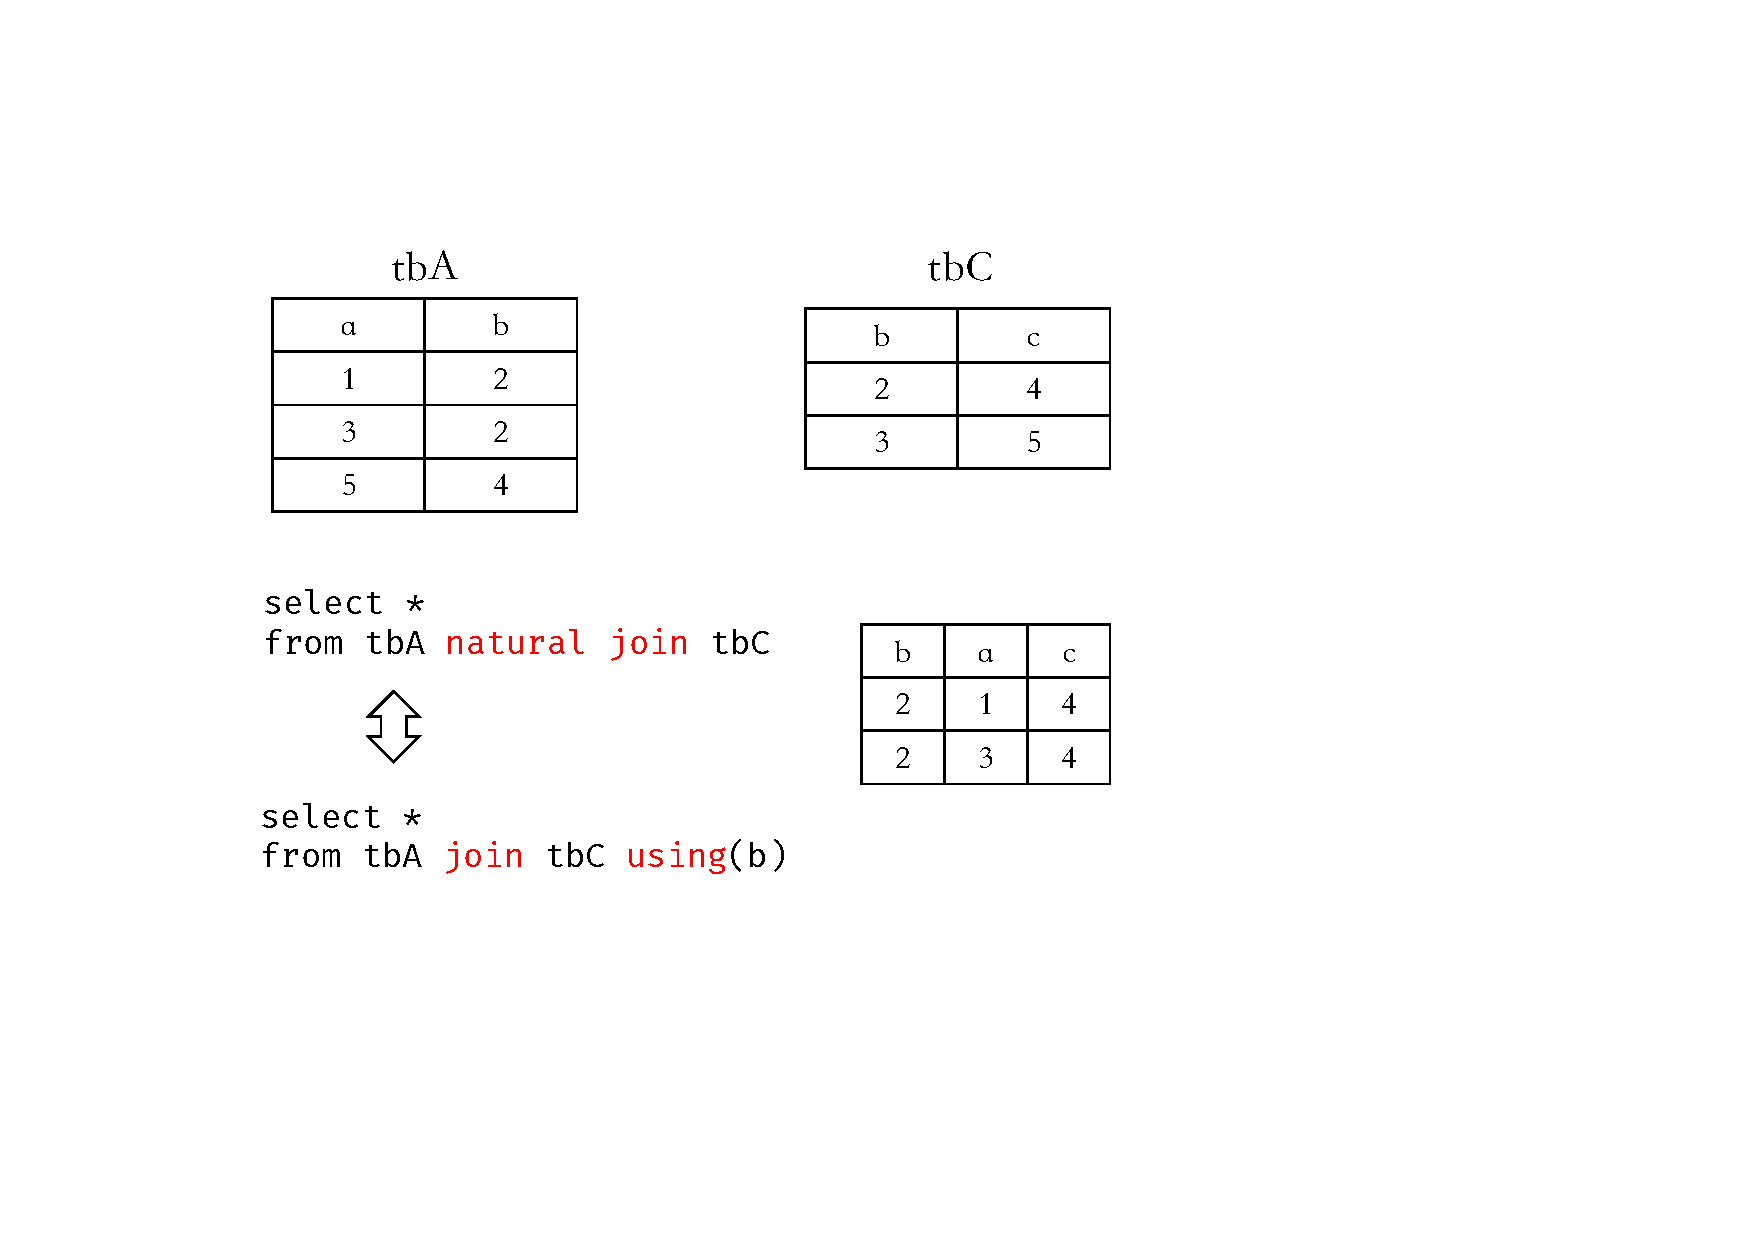
\includegraphics[width=.5\textwidth]{figure/natural_join.pdf}
    \caption{natural join}
\end{figure}

在某些数据库(如 MySQL)中, \verb|JOIN| 关键字默认等价于 \verb|INNER JOIN|, 但其他数据库(如 PostgreSQL)可能需要显式写 \verb|INNER JOIN|.

straight join:
默认情况下, MySQL 优化器会根据统计信息(如表大小、索引使用情况等)决定连接顺序. 
但在某些情况下, 优化器的选择可能不是最优的. 
此时, \verb|STRAIGHT_JOIN| 可以手动指定连接顺序, 确保左侧表作为驱动表.

\begin{lstlisting}[language=SQL, caption={多表连接}]
select *
from tbA A  inner join tbA B on A.b=B.b
            inner join tbA C on A.b=C.b

select *
from tbA A  join (tbA B, tbA C)
            on (A.b=B.b and A.b=C.b)
\end{lstlisting}

cross apply与outer apply: 提取左表中的每一行, 与右表中的所有行进行匹配.
\begin{figure}[H]
    \centering
    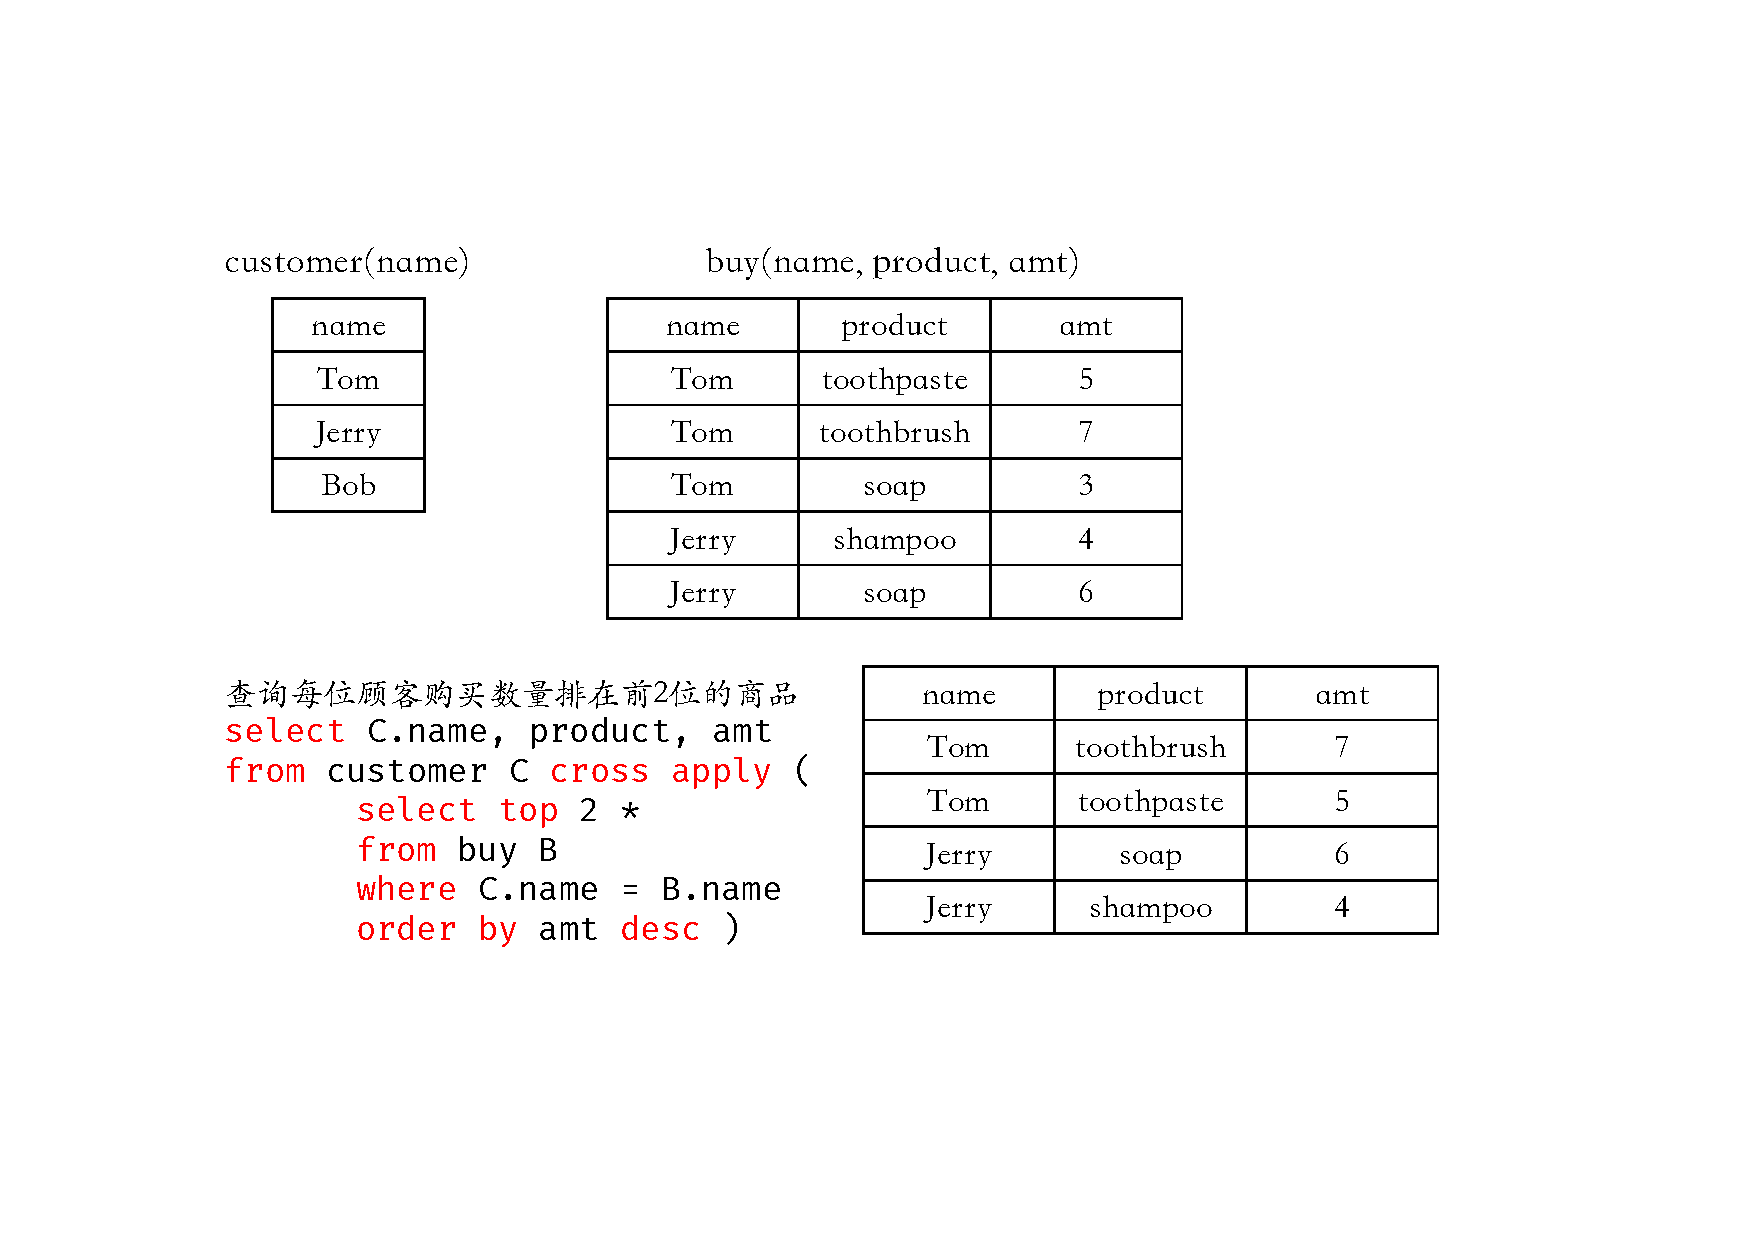
\includegraphics[width=.8\textwidth]{figure/cross_apply.pdf}
    \caption{cross apply示例}
\end{figure}

\subsection{集合运算}

\begin{itemize}
  \item 集合并: \verb|union (all)|
  \item 集合交: \verb|intersect (all)|
  \item 集合差: \verb|except (all)|
  \item 集合操作缺省去除重复元组
  \item \verb|intersect| 的优先级高于其他集合操作的优先级
  \item 加上 \verb|all| 表示当成 multi-set 来操作.
\end{itemize}

求工资大于1000或者年龄大于60的教工:
\begin{lstlisting}[language=SQL, caption={集合操作表达查询的例子}]
-- 查询 1
select tno
from teacher
where salary > 1000
union all
select tno
from teacher
where age > 60

-- 查询 2
select tno
from teacher
where salary > 1000
   or age > 60
\end{lstlisting}

上面的查询 1和查询 2等价, 但是查询 2的效率更高.

\begin{lstlisting}[language=SQL, caption={求出选修所有课程的同学}]
SELECT sno
FROM student S1
WHERE
  (
    -- 所有课程
    SELECT cno
    FROM C
    EXCEPT
    -- 除去学生选的课程
    SELECT cno
    FROM SC
    WHERE S1.sno = SC.sno
  ) IS NULL;
  -- 剩下的课程为 NULL
\end{lstlisting}

\subsection{聚集函数(Group function)}

\begin{itemize}
  \item 平均值: \verb|avg|
  \item 最小值: \verb|min|
  \item 最大值: \verb|max|
  \item 总和: \verb|sum|
  \item 记数: \verb|count|
\end{itemize}

\begin{lstlisting}[language=SQL, caption={聚集函数最容易犯的语法错误}]
select sno
from SC
where grade = max(grade)
-- Error Code: 1111. Invalid use of group function

-- 正确的使用方法
select sno
from SC
where grade = (select max(grade) from SC)
\end{lstlisting}

聚集函数处理null: \textcolor{red}{除了 \texttt{count} 之外忽略null.}

统计型聚集函数: \verb|std|, \verb|stddev|, \verb|stddev_pop|, \verb|stddev_samp|,
\verb|variance|, \verb|var_pop|, \verb|var_samp|.

\subsection{分组运算}

\verb|group by| 将表中行按指定列上值相等的原则分组, 然后在每一分组上使用聚集函数, 得到单一值.

\verb|having| 对分组进行选择, 只将聚集函数作用到满足条件的分组上.

\begin{lstlisting}[language=SQL]
-- 每门课程 所有同学的平均成绩
select avg(grade)
from SC

-- 特定同学的平均成绩
select avg(grade)
from SC
where sno = 's1'

-- 列出每个学生的最高、最低、平均成绩
select  sno,
        max(grade),
        min(grade),
        avg(grade)
from SC
group by sno
\end{lstlisting}

分组查询中各子句的顺序: where $\to$ group by $\to$ having.
\begin{lstlisting}[language=SQL]
-- 所有课程都及格了的同学的平均成绩
select sno, avg(grade)
from SC
group by sno
having min(grade) >= 60

-- 所有同学的及格了的课程的平均成绩
select sno, avg(grade)
from SC
where grade >=60
group by sno

-- 列出每一年龄组中男学生(超过50人) 的人数
select age, count(sno)
from student
where sex = 'M'
group by age
having count(*) > 50
\end{lstlisting}

\hyperlink{https://leetcode.cn/problems/sum-of-unique-elements/description/}{Leetcode 1748. 唯一元素的和}: \textit{给你一个整数数组 \texttt{nums}.数组中唯一元素是那些只出现恰好一次的元素.
请你返回 \texttt{nums} 中唯一元素的和.}

我们把原来的 \verb|nums| 数组放在表 \verb|numTb| 的 \verb|nums| 列之中.
\begin{lstlisting}[language=SQL]
select sum(nums)
from
  (select nums
   from numTb
   group by nums -- 按照 nums 的数值分组
   -- 如果组内只有一个, 说明是唯一元素
   having count(*)=1 ) tmpT
\end{lstlisting}


\begin{lstlisting}[language=SQL]
group_concat 列名
  [order by 排序列]
  [separator 分隔符]

insert into ds value  ('cs', 'bob'),
                      ('cs', 'tom'),
                      ('maths', 'mary'),
                      ('maths', 'lisa'),
                      ('maths', null);

select  dname,
        group_concat(sname)
from ds
group by dname

select  dname,
        group_concat(name order by sname)
from ds
group by dname

select  dname,
        group_concat(name order by separator ' | ')
from ds
group by dname
\end{lstlisting}

注意: $n$个属性的所有 \verb|group by|, 共有$2^n$个.

\textbf{Cube}: 其实是这样的, 假设我们$\texttt{group by }A_1,A_2,...,A_m$. 同时我们设每个属性上的Distinct的取值集合为$D_i(1\leq i\leq m)$.

那么, \verb|with cube| 会让每个属性在$\{\texttt{NULL}\}\cup D_i$上变化. 这样总共就是有:
\begin{align*}
    \prod_{i=1}^m (|D_i|+1).
\end{align*}

\begin{figure}[H]
    \centering
    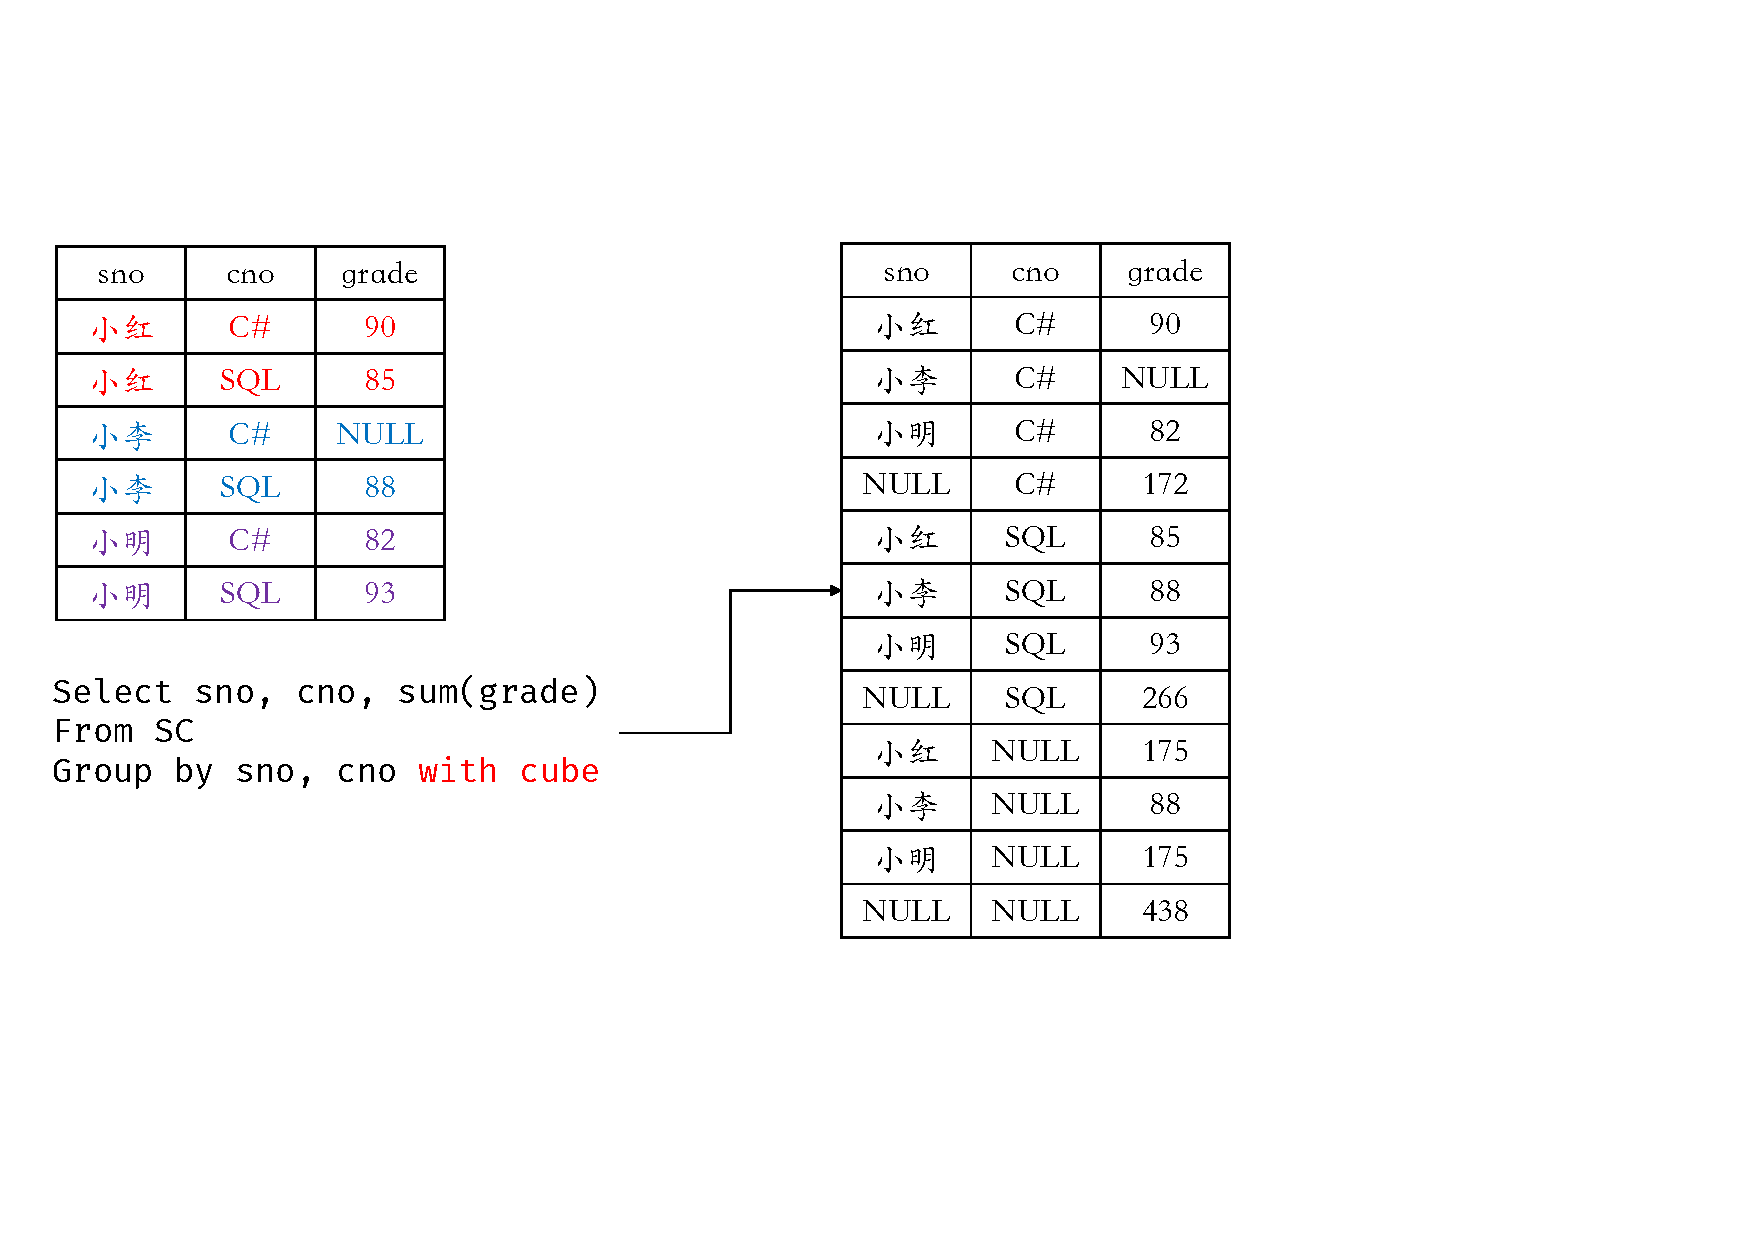
\includegraphics[width=.6\textwidth]{figure/with_cube.pdf}
    \caption{Cube示例}
\end{figure}

\begin{lstlisting}[language=SQL]
select Model, Year, Color, sum(Sales)
from car_sales
group by Model, Year, Color with cube
\end{lstlisting}

\textbf{Rollup}: 按照维度顺序统计. 例如$\texttt{group by }A_1,A_2,...,A_m$, 先不分组统计, 再按照$A_1$分组统计, 再按照$A_1,A_2$分组统计, ..., 最后按照分组$A_1,A_2,...,A_m$统计.

同时我们设每个属性上的Distinct的取值集合为$D_i(1\leq i\leq m)$.
那么Rollup产生的行数为:
\begin{align*}
    |D_1| + |D_1|\times |D_2| + |D_1|\times |D_2| \times |D_3| + \cdots + \prod_{i=1}^m |D_i| = \sum_{k=1}^m \prod_{i=1}^k |D_i|.
\end{align*}

只有 \verb|count(*)| 会把 null计入, 其他(包括 \verb|count(B)| 这样的)都不会计入.

group by将多个null行视为同一个分组.

\textbf{Grouping}: grouping是一个聚合函数, 它产生一个附加的列, 当用cube或rollup运算符添加行时, 附加
列的输出值为1, 否则为0.

\begin{lstlisting}[language=SQL]
select  if (grouping(A)=1, '汇总', '原始') grpA, A,
        if (grouping(B)=1, '汇总', '原始') grpB, B,
        count(*)
from group_null
group by A, B with rollup
\end{lstlisting}

对于grouping(A, B, C), 
\begin{itemize}
  \item 分组(A, B, C)的标识为4*0+2*0+1*0=0
  \item 分组(A, B)的标识为4*0+2*0+1*1=1
  \item 分组(A)的标识为4*0+2*1+1*1=3
  \item 分组()的标识为4*1+2*1+1*1=7
\end{itemize}

\textbf{Grouping sets}:
\begin{lstlisting}[language=SQL]
group by grouping sets
( (分组属性集1), (分组属性集2), ...(分组属性集n) )

select model, car_year, color, sum(sales)
from car_sales
group by grouping sets (
  (model, theyear),
  (model, color),
  (theyear, color),
  () )
\end{lstlisting}

\begin{align*}
&\texttt{cube}(a, b) = \texttt{grouping sets}((a, b), (a), (b), ()) \\
&\texttt{rollup}(x, y, z) = \texttt{grouping sets}((x, y, z), (x, y), (x), ()) \\
&\texttt{group by cube}(a, b), \texttt{rollup}(x, y, z) \\
&= \texttt{group by } \texttt{grouping sets}((a, b), (a), (b), ()), \texttt{grouping sets}((x, y, z), (x, y), (x), ()) \\
&= \texttt{group by grouping sets}((a, b, x, y, z), (a, b, x, y), (a, b, x), (a, b), \\
&\quad (a, x, y, z), (a, x, y), (a, x), (a), \\
&\quad (b, x, y, z), (b, x, y), (b, x), (b), \\
&\quad (x, y, z), (x, y), (x), ())
\end{align*}

\subsection{嵌套子查询}

\textbf{in子查询}. \verb|[not] in (子查询)|.

\begin{lstlisting}[language=SQL]
SELECT sname
FROM student S, SC
WHERE S.sno = SC.sno
  AND cno = 'c1';

SELECT sname
FROM student S
WHERE sno IN (
    SELECT sno
    FROM SC
    WHERE cno = 'c1'
);

-- 一般来说, 第 1 个查询更有效
\end{lstlisting}

\textbf{some/all子查询}:
\begin{itemize}
  \item 表达式 比较运算符$\theta$ some (子查询): 表达式的值至少与子查询结果中的一个值相比满足比较运算符$\theta$;
  \item 表达式 比较运算符$\theta$ all (子查询): 表达式的值与子查询结果中的所有的值相比都满足比较运算符$\theta$;
  \item =some就等价于in; $\neq$all就等价于not in.
\end{itemize}

\begin{lstlisting}[language=SQL, caption={找出平均成绩最高的学生号}]
select sno
from SC
group by sno
having avg(grade) >= all
        (select avg(grade)
        from SC
        group by sno)
\end{lstlisting}

\begin{lstlisting}[language=SQL, caption={找出每个系平均成绩最高的学生}]
select dno, S.sno
from student S, SC
where S.sno = SC.sno
group by dno, S.sno
having avg(grade) >= all
        (select avg(grade)
        from student X, SC
        where X.sno = SC.sno
        and X.dno = S.dno
        group by sno)
\end{lstlisting}

\textbf{exists子查询}: [not] exists (子查询). 判断子查询的结果集合中是否有任何元组存在.

\begin{itemize}
  \item in后的子查询与外层查询无关, 每个子查询执行一次, 称其为无关子查询.
  \item exists后的子查询与外层查询有关, 需要执行多次, 称之为相关子查询.
\end{itemize}

\begin{lstlisting}[language=SQL, caption={列出选修了c1号课程的学生姓名}]
select sname
from student S
where exists
      (select *
      from SC
      where cno = c1
      and sno = S.sno)
\end{lstlisting}

\begin{lstlisting}[language=SQL, caption={列出选修了c1号和c2号课程的学生的学号}]
select sno
from SC SC1
where SC1.cno = c1
  and exists
      (select sno
      from SC
      where cno = c2
      and sno = SC1.sno)
\end{lstlisting}

反半连接: not in, not exists.

列出没有选修课程的学生的姓名:
\begin{align*}
    \Pi_{sno}(S)-\Pi_{sno}(SC).
\end{align*}

\begin{lstlisting}[language=SQL]
select sname
from student
where sno not in
      (select sno
      from SC)

select sname
from student S
where not exists
      (select sno
      from SC
      where sno=S.sno)
\end{lstlisting}

ps. 这里后面介绍了除法 和 not exists ... not exists 的关系.

\subsection{字符串与文本操作}

LIKE 操作符:
\begin{lstlisting}[language=SQL]
SELECT * FROM table_name 
WHERE column_name LIKE pattern;
-- 查找以 "A" 开头的所有名字
SELECT * FROM users WHERE name LIKE 'A%';

-- 查找第二个字符是 "o" 的三字名字
SELECT * FROM users WHERE name LIKE '_o_';

-- 查找包含 "cat" 的名字
SELECT * FROM users WHERE name LIKE '%cat%';
\end{lstlisting}


REGEXP:
\begin{lstlisting}[language=SQL]
SELECT * FROM table_name 
WHERE column_name REGEXP pattern;

-- 查找以 "A" 开头且以 "e" 结尾的名字
SELECT * FROM users WHERE name REGEXP '^A.*e$';

-- 查找包含连续三个数字的名字
SELECT * FROM users WHERE name REGEXP '[0-9]{3}';

-- 查找格式为 "XXX-XXX-XXXX" 的电话号码
SELECT * FROM contacts WHERE phone REGEXP '^[0-9]{3}-[0-9]{3}-[0-9]{4}$';
\end{lstlisting}

\section{数据更新}

\begin{remark}
  期末考试不考!!!
\end{remark}

INSERT、DELETE、TRUNCATE、UPDATE、OUTPUT、MERGE.

\begin{lstlisting}[language=SQL]
-- 插入单条记录
INSERT INTO employees (name, age, department) 
VALUES ('John Doe', 28, 'Engineering');

-- 批量插入
INSERT INTO students (class_id, name, gender, score) 
VALUES 
  (1, '大宝', 'M', 87),
  (2, '二宝', 'M', 81);

-- 删除特定记录
DELETE FROM employees WHERE employee_id = 100;

-- 删除所有记录(危险操作!)
DELETE FROM employees;

TRUNCATE TABLE logs; -- 清空 logs 表的所有数据

-- 更新单列
UPDATE employees 
SET department = 'Senior Engineering' 
WHERE age > 30;

-- 更新多列
UPDATE customers 
SET cust_contact = 'Sam Roberts', cust_email = 'sam@toyland.com'
WHERE cust_id = '1000000006';

-- 删除记录并返回被删除的数据
DELETE FROM orders 
OUTPUT DELETED.order_id, DELETED.customer_id
WHERE order_date < '2023-01-01';

-- 合并订单数据:匹配则更新,否则插入
MERGE INTO orders AS target
USING (SELECT * FROM temp_orders) AS source
ON target.order_id = source.order_id
WHEN MATCHED THEN 
  UPDATE SET target.amount = source.amount
WHEN NOT MATCHED THEN 
  INSERT (order_id, amount) VALUES (source.order_id, source.amount);
\end{lstlisting}

\section{服务器端脚本语言}

\textcolor{red}{主要掌握游标和触发器的定义和使用!!!}

\subsection{SQL脚本语法成分}

\begin{enumerate}
    \item 局部变量: 使用 \verb|DECLARE| 声明变量, 以 \verb|@| 开头(如 \verb|@var|). 赋值可通过 \verb|SET| 或 \verb|SELECT|.
\begin{lstlisting}[language=SQL]
DECLARE @Name NVARCHAR(50) = 'Alice';
DECLARE @Counter INT = 0;
SET @Counter = 1;
SELECT @Name = Name FROM Users WHERE UserID = 1;
\end{lstlisting}
    \item 控制流:
    \begin{enumerate}
        \item 条件判断: \verb|IF...ELSE...| 和 \verb|CASE|.
\begin{lstlisting}[language=SQL]
IF @Age >= 18
    PRINT 'Adult';
ELSE
    PRINT 'Minor';

SELECT 
    Name,
    Status = CASE 
        WHEN Salary > 10000 THEN 'High'
        WHEN Salary > 5000 THEN 'Medium'
        ELSE 'Low'
    END
FROM Employees;
\end{lstlisting}
        \item 循环结构: \verb|WHILE| 和 \verb|LOOP ... LEAVE / ITERATE|.
\begin{lstlisting}[language=SQL]
DECLARE @i INT = 1;
WHILE @i <= 5
BEGIN
    PRINT 'Iteration ' + CAST(@i AS NVARCHAR);
    SET @i += 1;
END
\end{lstlisting}
    \end{enumerate}
      \item 异常处理, 使用 \verb|TRY...CATCH|.
\begin{lstlisting}
BEGIN TRY
    UPDATE Accounts SET Balance = Balance - 100 WHERE AccountID = 1;
    UPDATE Accounts SET Balance = Balance + 100 WHERE AccountID = 2;
END TRY
BEGIN CATCH
    ROLLBACK;
    PRINT 'Error: ' + ERROR_MESSAGE();
END CATCH
\end{lstlisting}
  \item 游标(Cursor).
\begin{lstlisting}[language=SQL]
-- 1. 声明游标
DECLARE employee_cursor CURSOR FOR
SELECT EmployeeID, Name FROM Employees WHERE Department = 'Sales';

-- 2. 打开游标
OPEN employee_cursor;

-- 3. 声明变量存储提取的数据
DECLARE @EmpID INT, @Name NVARCHAR(50);

-- 4. 提取数据并处理
FETCH NEXT FROM employee_cursor INTO @EmpID, @Name;
WHILE @@FETCH_STATUS = 0
BEGIN
    PRINT 'Employee ID: ' + CAST(@EmpID AS NVARCHAR) + ', Name: ' + @Name;
    FETCH NEXT FROM employee_cursor INTO @EmpID, @Name;
END

-- 5. 关闭游标
CLOSE employee_cursor;

-- 6. 释放游标
FREE employee_cursor;
\end{lstlisting}
  \item 动态 SQL.
\begin{lstlisting}[language=SQL]
DECLARE @SQL NVARCHAR(MAX);
SET @SQL = 'SELECT * FROM Users WHERE Name = ''Alice''';
EXEC(@SQL);

DECLARE @SQL NVARCHAR(MAX), @Name NVARCHAR(50) = 'Alice';
SET @SQL = N'SELECT * FROM Users WHERE Name = @Name';
EXEC sp_executesql @SQL, N'@Name NVARCHAR(50)', @Name;
\end{lstlisting}
\end{enumerate}

\subsection{服务器端 SQL 脚本形式}

\begin{enumerate}
    \item 批处理(Batch).一组 SQL 语句的集合, 通过 \verb|GO| 分隔.
\begin{lstlisting}[language=SQL]
-- GO 是 SQL Server 的批处理分隔符(非 SQL 标准)
DECLARE @Msg NVARCHAR(50) = 'Hello';
PRINT @Msg;
GO
PRINT @Msg; -- 错误:@Msg 作用域仅在第一个批处理中
\end{lstlisting}
    \item 存储过程(Stored Procedure): 预编译的 SQL 代码块, 可接受输入/输出参数.
\begin{lstlisting}[language=SQL]
CREATE PROCEDURE usp_GetEmployee
    @ID INT
AS
BEGIN
    SELECT * FROM Employees WHERE EmployeeID = @ID;
END

EXEC usp_GetEmployee @ID = 1;
\end{lstlisting}
  \item 函数(Function): 标量函数(返回单个值), 表值函数(返回表结果集).
\begin{lstlisting}
CREATE FUNCTION dbo.GetAge(@DOB DATE)
RETURNS INT
AS
BEGIN
    RETURN DATEDIFF(YEAR, @DOB, GETDATE());
END

SELECT dbo.GetAge('2000-01-01');

CREATE FUNCTION dbo.GetEmployeesByDept(@Dept NVARCHAR(50))
RETURNS TABLE
AS
RETURN SELECT * FROM Employees WHERE Department = @Dept;

SELECT * FROM dbo.GetEmployeesByDept('Sales');
\end{lstlisting}
  \item 触发器(Trigger): 在表的 \verb|INSERT|, \verb|UPDATE|, \verb|DELETE| 操作前后自动执行的代码.
\begin{lstlisting}[language=SQL]
CREATE TRIGGER trg_AuditLog
ON Employees
AFTER UPDATE
AS
BEGIN
    INSERT INTO AuditLog (Action, Timestamp)
    VALUES ('Update', GETDATE());
END
\end{lstlisting}
\end{enumerate}
 

\chapter{关系中的非关系数据}

大数据分为:
\begin{enumerate}
    \item 结构化数据. \textit{指关系型数据表.}
    \item 半结构化数据. \textit{指关系结构与内容混合在一起的数据类型.}
    \item 非结构化数据. \textit{文档、视频、音频、图片.}
\end{enumerate}

\section{递归查询}

\subsection{层次结构的关系表示}

邻接表: \verb|Adjacent(child, parent)|.

物化路径: \verb|material_path(node, path)|. 从起点出发的路径.

嵌套集合: \verb|nestedSet(node, left_value, right_value)|. \textit{嵌套集模型是根据树遍历来对节点进行编号,遍历会访问每个节点两次,按访问顺序分配数字,并在两次访问中都分配.这将为每个节点留下两个数字,它们作为节点两个属性存储.这使得查询变得高效:通过比较这些数字来获得层级结构关系.但是更新数据将需要给节点重新分配数字,因此变得低效.}

\subsection{递归查询}

层次结构的传递闭包: 使用递归查询.

\begin{figure}[H]
    \centering
    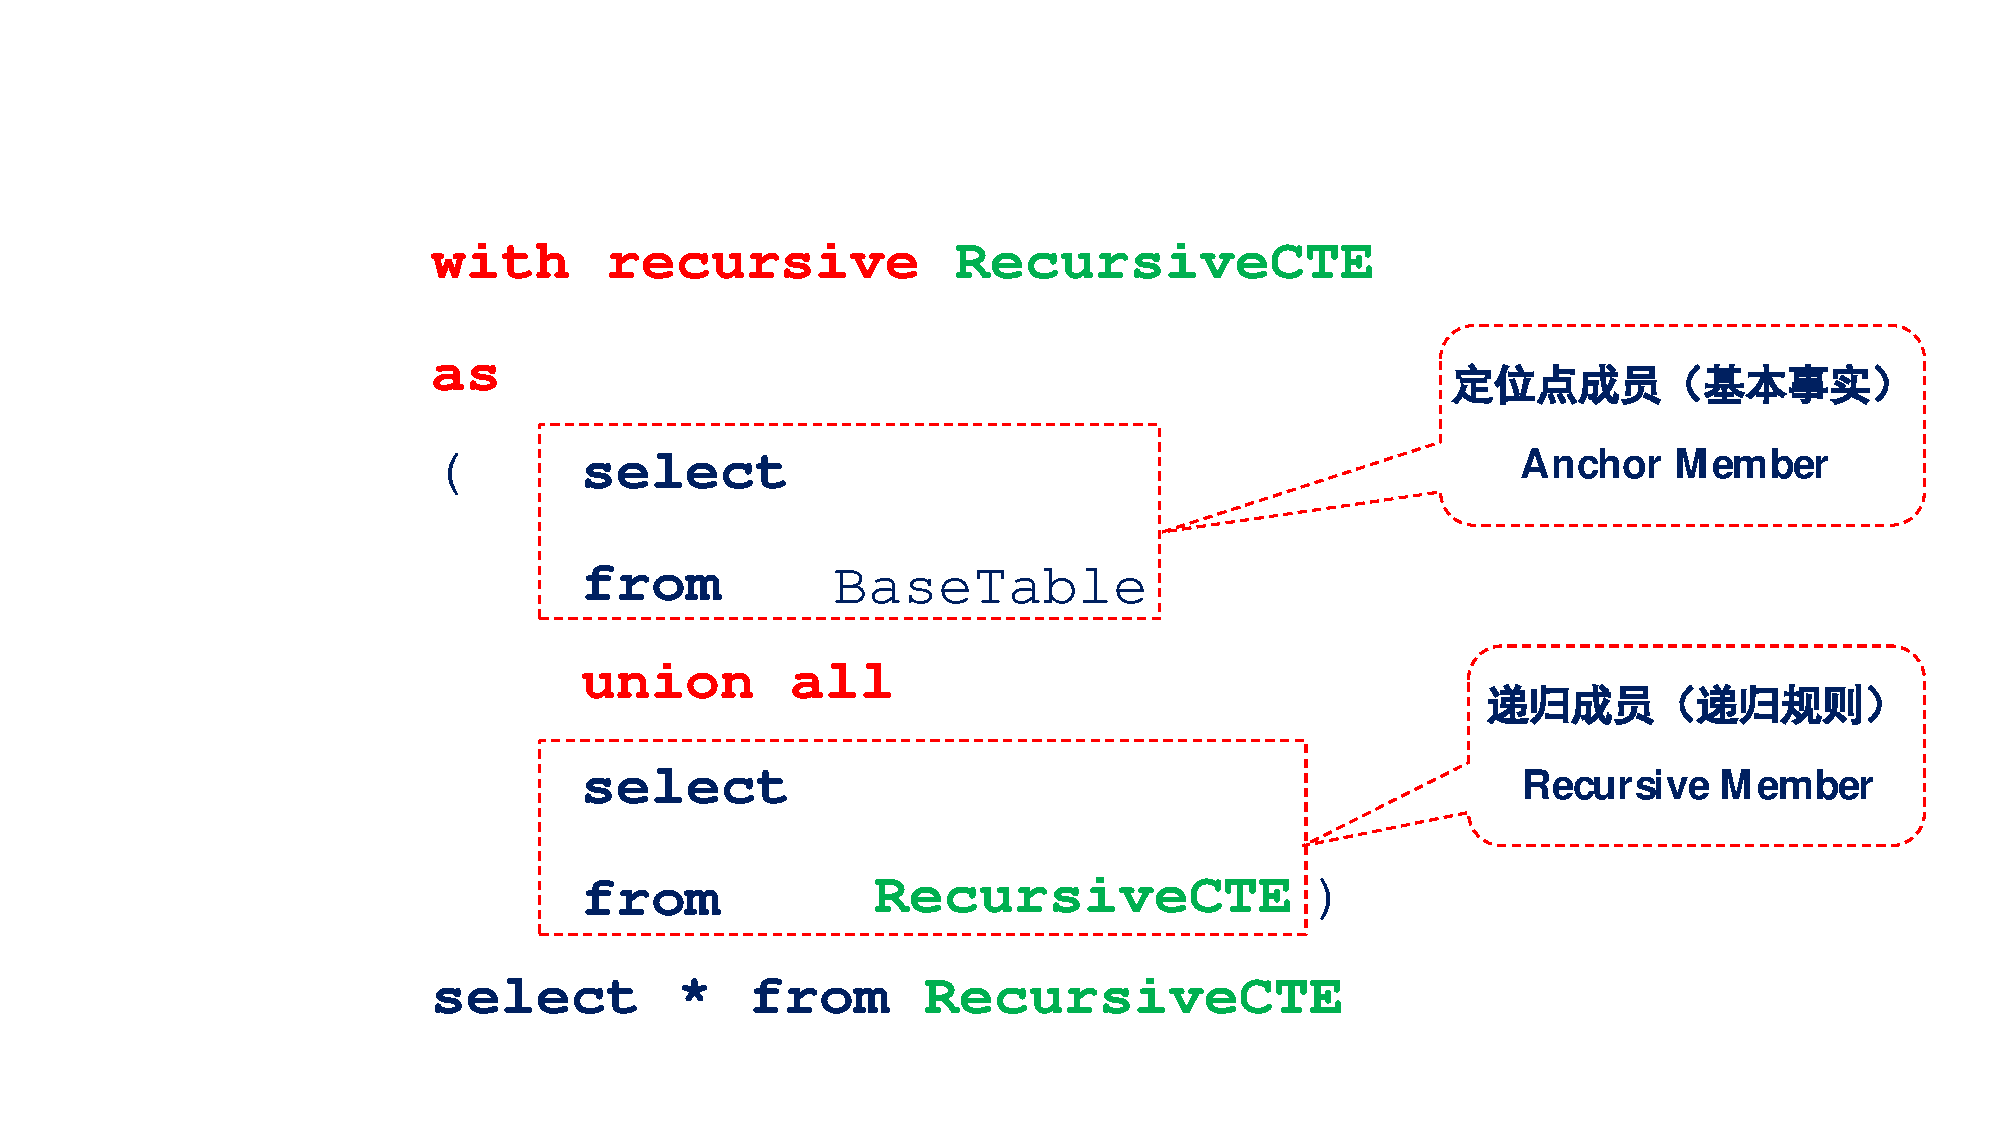
\includegraphics[width=.4\textwidth]{./image/递归查询.pdf}
    \caption{MySQL中的递归查询}
\end{figure}

\begin{lstlisting}[language=SQL]
with recursive nums(n)
as
(   select 1
    union all
    select n+1
    from nums
    where n < 100 )
select sum(n) from nums
\end{lstlisting}

\begin{lstlisting}[language=SQL]
with recursive Components ( part, subpart )
as
( select part, subpart
  from Assembly
  union all
  select A.part, C.subpart
  from Assembly A, Components C
  where A.subpart = C.part )
  select * from Components where part = 'trike'
\end{lstlisting}

\begin{example}
    利用递归查询计算经理下属. 表结构: emp(empid, ename, mgrid).
\end{example}

\begin{lstlisting}[language=SQL]
declare @root = 1 as int
-- 定义递归起点编号
with recursive SubsCTE
as ( select empid, ename, 0 as lvl
     from emp
     where empid = @root
     -- 初始查询
     union all
     select C.empid, C.ename, P.lvl + 1
     from SubsCTE as P join emp AS C on C.mgrid = P.empid
     -- 查询当前层级的表: SubsCTE
      )
select * from SubsCTE    
\end{lstlisting}

\begin{lstlisting}[language=SQL]
declare @lvl = 0 as int
create temporary table Subs( empid int, level int )
-- 插入根节点
insert into Subs( empid, level )
    select empid, @lvl from emp
    where empid = @root;
while found_rows() > 0

-- 递归查找下属
begin
    set @lvl = @lvl + 1
    insert into Subs( empid, level )
        select C.empid, @lvl
        from Subs as P join emp as C
        on P.lvl = @lvl - 1 and C.mgrid = P.empid
end    
\end{lstlisting}

\begin{figure}[H]
    \centering
    \includegraphics[width=.6\textwidth]{./figure/递归查询.pdf}
    \caption{Oracle中的递归查询}
\end{figure}

\subsection{层次结构典型查询问题}

树形结构(数据存放在邻接表中)
\begin{enumerate}
    \item 返回给定节点的所有下属,并标注层级
    \item 返回给定节点的所有上级,并标注层级
    \item 移动子树,将一颗子树的根节点换成另外一个
    \item 将邻接表转换为物化路径,并存放在一个表中
    \item 基于物化路径表,查询指定节点的所有子节点
    \item 基于物化路径表,查询指定节点的所有父节点
    \item 将邻接表转换为嵌套集合,并存放在一个表中
    \item 基于嵌套集合表,查询指定节点的所有子节点
    \item 基于嵌套集合表,查询指定节点的所有父节点
\end{enumerate}

图
\begin{enumerate}
    \item 计算传递闭包
    \item 计算最短路径
    \item 环路检测
\end{enumerate}

\section{XML}

\begin{enumerate}
    \item 标签(tag): 定义数据成为一个元素.
    \item 文本(text): 说明元素属性.
    \item 元素(elements): \texttt{<起始标签>元素属性<结束标签>}的组合.
\end{enumerate}

格式正确的(well-formed)XML文档
\begin{enumerate}
    \item 只能有唯一的根元素
    \item 所有元素都必须有起始标签和结束标签
    \item 大小写一致, XML区分大小写
    \item 子元素必须被上层元素完全包含
    \item 属性值必须被双引号或单引号括起来
    \item 元素内的属性不能被重复使用
\end{enumerate}

\begin{lstlisting}[language=XML]
<books>
    <book id="0001">
        <bookname> 数据库技术</bookname>
    </book>
    <book id="0001">
        <bookname> 数据仓库技术</bookname>
    </book>
</books>
\end{lstlisting}

HTML: HyperText Markup Language. 描述数据的显示格式

XML: eXtensible Markup Language. 描述数据的内容

XML: 半结构化模型的资源描述框架. RDF (Resource Description Framework)

存储RDF使用三元组: \texttt{<标识符, 属性名, 属性值>}. 或者\texttt{<Subject, Property, Object>}.

基于三元组表的RDF查询:
Implementation Techniques for Main Memory Databases喜欢什么和不喜欢什么?
\begin{lstlisting}[language=SQL]
SELECT    C.object, D.object
FROM      triples A, triples B, triples C, triples D
-- 四张相同的表triples, 别名分别为A, B, C, D
WHERE     A.subject = B.object
  AND     A.property = "title"
  AND     A.object = "Implementation Techniques for Main Memory Databases"
  -- A中找到标题为给出标题的对象.
  AND     B.property = "authorOf"
  -- B中找到authorOf A找出的书, 也就是找出作者
  AND     B.subject = C.subject
  AND     C.property = "likes"
  -- C中找出这个作者喜欢的东西
  AND     C.subject = D.subject
  AND     D.property = "dislikes"
  -- D中找出这个作者不喜欢的东西
\end{lstlisting}

三元组的\textcolor{red}{单属性表}表示: 过于细碎, 导致太多的连接操作.

三元组的\textcolor{red}{宽表}表示: 太多列+稀疏.

DTD(Document Type Definition)是XML的核心机制之一, 用于定义XML文档的结构和规则.
它的主要作用是:
\begin{enumerate}
    \item 验证 XML 文档的合法性: 确保 XML 文档的元素、属性、内容等符合预定义的结构规则.
    \item 约束文档格式: 通过定义元素的嵌套关系、属性的取值范围等, 保证数据的一致性和正确性.
    \item 支持数据交换: 为不同系统之间共享数据提供统一的结构规范.
\end{enumerate}

\begin{lstlisting}[language=XML]
<?xml version="1.0" encoding="UTF-8"?>
<!DOCTYPE note [
    <!ELEMENT note (to,from,heading,body)>
    <!ELEMENT to (#PCDATA)>
    <!ELEMENT from (#PCDATA)>
    <!ELEMENT heading (#PCDATA)>
    <!ELEMENT body (#PCDATA)>
]>
<note>
    <to>Tove</to>
    <from>Jani</from>
    <heading>Reminder</heading>
    <body>Don't forget me this weekend!</body>
</note>
\end{lstlisting}

每个DTD规则表达式是一个有限状态自动机.
\begin{lstlisting}[language=XML]
<!ELEMENT books (book+)>
<!ELEMENT book (title, author+, year, price)>
<!ATTLIST book id ID #REQUIRED>
<!ELEMENT title (#PCDATA)>
<!ELEMENT author (#PCDATA)>
<!ELEMENT year (#PCDATA)>
<!ELEMENT price (#PCDATA)>
<!ENTITY company "MyPublisher">
\end{lstlisting}

XML数据模型(DOM, Document Object Model)是 W3C(万维网联盟)制定的一种标准接口规范, 
用于动态访问和操作 XML 或 HTML 文档的内容、结构和样式. 
它是通过将文档解析为树形结构(即 DOM 树), 并以对象的形式表示每个节点(如元素、属性、文本等), 
从而允许程序或脚本以编程方式操作文档.

XPath (XML Path Language)是一种用于在 XML 或 HTML 文档中定位和选择节点的查询语言.
它通过路径表达式(Path Expressions)和条件筛选(谓语)来导航 XML 文档的树形结构, 
从而提取特定的数据或节点.


\begin{table}[H]
    \centering
    \begin{tabular}{|l|l|l|}
    \hline
    \textbf{表达式} & \textbf{含义} & \textbf{示例} \\
    \hline
    / & 从根节点开始选取 & /bookstore/book \\
    \hline
    // & 从当前节点开始,选取文档中任意位置的节点 & //title \\
    \hline
    . & 当前节点 & .//price \\
    \hline
    .. & 父节点 & ../author \\
    \hline
    @ & 选取属性 & @id \\
    \hline
    \end{tabular}
    \caption{路径表达式}
\end{table}

\begin{table}[H]
    \centering
    \begin{tabular}{|l|l|l|}
    \hline
    \textbf{表达式} & \textbf{含义} & \textbf{示例} \\
    \hline
    * & 选取所有子节点 & /* (根节点的所有子元素) \\
    \hline
    @* & 选取所有属性 & //@lang \\
    \hline
    text() & 选取文本节点 & //price/text() \\
    \hline
    \end{tabular}
    \caption{节点选择}
\end{table}

谓语(条件筛选):
\begin{itemize}
    \item \textbf{索引筛选}: [n] 选择第 n 个节点(从 1 开始计数):
    \begin{verbatim}
/bookstore/book[1]  % 第一个 book 节点
    \end{verbatim}
    \item \textbf{属性筛选}: [@属性名='值']:
    \begin{verbatim}
//book[@id='b001']  % id 为 b001 的 book 节点
    \end{verbatim}
    \item \textbf{文本筛选}: [text()='值'] 或 contains(text(), '部分值'):
    \begin{verbatim}
//title[text()='XML权威指南']  % 文本完全匹配
//title[contains(text(), '指南')]  % 文本包含 "指南"
    \end{verbatim}
\end{itemize}

\begin{table}[H]
    \centering\begin{tabular}{|l|l|l|}
        \hline
        \textbf{轴} & \textbf{含义} & \textbf{示例} \\
        \hline
        child:: & 子元素(默认可省略) & child::book (等价于 book) \\
        \hline
        parent:: & 父节点 & parent::bookstore \\
        \hline
        ancestor:: & 所有祖先节点 & ancestor::bookstore \\
        \hline
        descendant:: & 所有后代节点 & descendant::title \\
        \hline
        following-sibling:: & 所有后续兄弟节点 & following-sibling::author \\
        \hline
    \end{tabular}
    \caption{轴(Axis)}
\end{table}


MySQL中的XML函数: \verb|ExtractValue(xml_target, xpath_expr)|, 从 XML 数据中提取特定节点的值.
\begin{lstlisting}[language=SQL]
-- 提取 <to> 节点的值
SELECT ExtractValue('<note><to>Tove</to></note>', '/note/to');
-- 结果: Tove

-- 提取多个节点的值(使用 `|` 分隔)
SELECT ExtractValue('<a><b>1</b><c>2</c></a>', '//b/text() | //c/text()');
-- 结果: 1 2
\end{lstlisting}

\section{JSON}

JSON的基本成分为:
\begin{enumerate}
    \item 对象. \verb|{属性名: 属性值, 属性名: 属性值}|. E.g., \verb|{'name': 'Tom', 'hobby': ['sing', 'dance']}|.
    \item 数组. \verb|[value, value, value ...]|. \verb|[{'name': 'Tom', 'age': 12}, {...}]|.
\end{enumerate}

MySQL中生成JSON的函数:
\begin{enumerate}
    \item \texttt{JSON\_ARRAY} 函数. 创建一个 JSON 数组.
    \begin{verbatim}
JSON_ARRAY(val1, val2, ..., valN)
    \end{verbatim}
    \begin{verbatim}
SELECT JSON_ARRAY(1, 'apple', NULL, TRUE);
-- 输出: [1, "apple", null, true]
    \end{verbatim}
    \item \texttt{JSON\_OBJECT} 函数. 将键值对列表返回为JSON对象.
    \begin{verbatim}
JSON_OBJECT('key1' VALUE val1, 'key2' VALUE val2, ...)
    \end{verbatim}
    \begin{verbatim}
SELECT JSON_OBJECT('id' VALUE 1, 'name' VALUE 'Alice');
-- 输出: {"id": 1, "name": "Alice"}
    \end{verbatim}
\end{enumerate}

MySQL中的JSON数据类型:
\begin{lstlisting}[language=SQL]
CREATE TABLE testJSON (
    a JSON,
    b INT
);
INSERT INTO testJSON VALUES
('[3, 10, 5,"x", 44]', 33),
('[3, 10, 5, 17,[22,"y", 66]]', 0);
-- 提取嵌套值
SELECT a->"$[3]", a->"$[4][1]" FROM testJSON;
-- 结果分别为: ["x", 17], [NULL, "y"]
\end{lstlisting}

JSON的检索操作:
\begin{lstlisting}[language=SQL]
create table user (
    id int not null primary key auto_increment,
    info json );
insert into user(info) values (
    '{"name":"wangming",
      "age":18,
      "address":{"province":"sichuan","city":"chengdu"},
      "hobby" :["sing", "dance"]}' );

-- 提取多层嵌套值
SELECT json_extract('[10, 20, [30, 40]]', '$[2][*]');
-- 输出: [30, 40]

-- 提取 JSON 对象中的字段
SELECT json_extract(info, '$.address.city') FROM user;
-- 输出: "chengdu"

-- 提取多个字段
SELECT json_extract(info, '$.name', '$.hobby') FROM user;
-- 输出: ["wangming", ["sing", "dance"]]
\end{lstlisting}

将JSON展开为平面表:
\begin{lstlisting}[language=SQL]
-- 展开 JSON 数组为行
SELECT *
FROM json_table(
    '[{"a":"3"},{"a":2},{"b":1},{"a":0},{"a":[1,2]}]',
    "$[*]"
    COLUMNS(
        rowid FOR ORDINALITY,
        ac VARCHAR(100) PATH "$.a" DEFAULT '111' ON EMPTY DEFAULT '999' ON ERROR,
        aj JSON PATH "$.a" DEFAULT '{"x": 333}' ON EMPTY,
        bx INT EXISTS PATH "$.b"
    )
) AS tt;
\end{lstlisting}
上面展开后的结果为:
\begin{table}[H]
    \centering
    \begin{tabular}{|l|l|l|l|}
        \hline
        rowid & ac & aj & bx \\ \hline
        1 & 3 & "3" & 0 \\ \hline
        2 & 2 & 2 & 0 \\ \hline
        3 & 111 & \{"x": 333\} & 1 \\ \hline
        4 & 0 & 0 & 0 \\ \hline
        5 & 999 & [1, 2] & 0 \\ \hline
    \end{tabular}
\end{table}

将JSON展开为平面表: 数组的unwind操作.
\begin{lstlisting}[language=SQL]
-- 展开 JSON 中的嵌套数组(类似 unwind 操作)
SELECT *
FROM json_table(
    '[{"a": 1, "b": [11, 111]}, {"a": 2, "b": [22, 222]}, {"a": 3}]',
    "$[*]"
    COLUMNS(
        a INT PATH "$.a",
        NESTED PATH "$.b[*]" COLUMNS(b INT PATH "$")
    )
) AS jt
WHERE b IS NOT NULL;
\end{lstlisting}

将平面表转换为JSON:
\begin{lstlisting}[language=SQL]
-- 将平面表转换为 JSON 数组
CREATE TABLE score (
    sname CHAR(10),
    cname CHAR(10),
    score INT
);

INSERT INTO score VALUES
('张三', '数学', 96),
('张三', '语文', 99),
('李四', '数学', 98),
('李四', '语文', 88);

-- 转换为 JSON 数组
SELECT CONCAT(
    '[',
    GROUP_CONCAT(
        json_object('sname' VALUE sname, 'cname' VALUE cname, 'score' VALUE score)
    ),
    ']'
) AS scores
FROM score;
\end{lstlisting}

\section{向量}

向量嵌入使得我们具有处理非结构化数据的能力.

向量数据库中的核心问题: 近似最近邻查找. ANN (Approximate nearest neighbor search)

多维索引使用k-d tree: \href{https://oi-wiki.org/ds/kdt/}{k-d树文档}

近似最近邻搜索算法 ANNOY: \cite{liApproximateNearestNeighbor2016}.

高维数据的搜索: HNSW: Hierarchical Navigable Small World \cite{malkovEfficientRobustApproximate2018}.

基于PostgreSQL的向量插件: pgvector (基于IVFFlat索引), pg\_embedding (基于HNSW索引).
\begin{lstlisting}[language=SQL]
-- 1. 启用插件
CREATE EXTENSION vector;

-- 2. 创建表
CREATE TABLE items (
    id bigserial PRIMARY KEY,
    embedding vector(3)
);

-- 3. 插入数据
INSERT INTO items (embedding) VALUES
    ('[1,2,3]'),
    ('[4,5,6]');

-- 4. 创建索引(IVFFlat)
CREATE INDEX idx_items_embedding_ivfflat 
ON items 
USING ivfflat (embedding vector_l2_ops) 
WITH (lists = 100);

-- 5. 查询相似向量
SELECT * 
FROM items 
ORDER BY embedding <=> '[3,1,2]' 
LIMIT 5;
\end{lstlisting} % FINISHED.

\chapter{关系规范化}

\section{关系模式的设计问题}

信息在关系模式中的表示完全取决于主码。

\begin{table}[H]
  \centering
  \begin{tabular}{|c|c|c|}
    \hline
    \textbf{职工} & \textbf{级别} & \textbf{工资} \\
    \hline
    赵明 & 4 & 500 \\
    \hline
    钱广 & 5 & 600 \\
    \hline
    孙志 & 6 & 700 \\
    \hline
    李开 & 5 & 600 \\
    \hline
    周祥 & 6 & 700 \\
    \hline
  \end{tabular}
  \caption{职工信息表}
\end{table}


\begin{enumerate}
    \item 信息的不可表示问题。
    \begin{enumerate}
        \item 插入异常:如果没有职工具有8级工资,则8级工资的工资数额就难以插入。
        \item 删除异常:如果仅有职工赵明具有4级工资,删除赵明则会将有关4级工资的工资数额信息也一并删除。
    \end{enumerate}
    \item 信息的冗余问题.
    \begin{enumerate}
        \item 数据冗余:职工很多,工资级别有限,每一级别的工资数额反复存储多次。
        \item 更新异常:如果将5级工资的工资数额调为620,则需要找到每个具有5级工资的职工,逐一修改。
    \end{enumerate}
\end{enumerate}

\ 

\fbox{职工}$\to$\fbox{级别}$\to$\fbox{工资}。\textbf{分解}为:\fbox{职工}$\to$\fbox{级别} + \fbox{级别}$\to$\fbox{工资}。

\section{函数依赖}

\begin{definition}[函数依赖] \label{def:func-dep}
  设$R(U)$是属性集$U$上的关系模式, $X,Y\subseteq U$, $r$是$R(U)$上的任意一个关系, 如果成立:
  \begin{center}
    对$\forall t,s\in r$, 若$t[X]=s[X]$, 则$t[Y]=s[Y]$
  \end{center}
  则称``$X$函数决定$Y$''或者``$Y$函数依赖于$X$'', 记作$X\to Y$. 称$X$为决定因素.
\end{definition}

例如, $sno\to sname$, $(sno, cno)\to grade$.

\begin{definition}[函数依赖的双重否定形式的定义] \label{def:func-dep-2}
  不存在$t,s\in r$, $t[X]=s[X]$, 但$t[Y]\neq s[Y]$.
\end{definition}

\begin{definition}[平凡的函数依赖] \label{def:pingfan-func-dep}
  如果$X\to Y$, $Y\subseteq X$, 则称其为平凡的函数依赖. 否则称为非平凡的函数依赖.
\end{definition}

如, $(sno,sname)\to sname$是平凡的函数依赖.

\textit{一个关系模式有$n$个属性,在它上面成立的所有可能的函数依赖有多少个?非平凡的函数依赖有多少个?}

\textbf{Answer.} 需要计算$X\to Y$的个数. 其中$X$和$Y$都是非空子集, 这就可以知道答案为$(2^n-1)^2$.  先计算出平凡的函数依赖个数. 也就是$Y\subseteq X$的个数, $\sum_{k=1}^{n} \binom{n}{k} (2^k-1)=3^n-2^n$. 接着减去这个数, 得到: $2^{2n}-2^n-3^n+1$.


\begin{definition}[完全函数依赖] \label{def:tot-func-dep}
  如果$X\to Y$, 且对于任意$X$的真子集$X'$, 都有$X' \nrightarrow Y$, 则称$Y$对$X$完全函数依赖, 记作$X\overset{f}{\rightarrow} Y$. 否则称$Y$对$X$部分函数依赖, 记作$X\overset{p}{\rightarrow}Y$.
\end{definition}

\begin{definition}[传递函数依赖] \label{def:trans-func-dep}
  在$R(U)$中, 如果: $X\to Y$, $Y\to Z$, $Y\nrightarrow X$, 且$Z\nsubseteq Y$, 则称$Z$对$X$传递函数依赖.
\end{definition}

\begin{remark}
  定义\ref{def:trans-func-dep}中$Y\nrightarrow X$意味着必须通过$Y$来传递, 而$Z\nsubseteq Y$说明并非平凡依赖, 否则可以直接导出$X\to Z$.
\end{remark}

主要问题:如果关系模式设计不当,把本来彼此没有依赖关系的两个属性放在同一个关系模式中,所造成的对候选码的部分依赖和传递依赖是在现实中不存在的,从而会出现异常。
\textit{E.g., 学号$\to$系号, 系号$\to$系主任, 这样学号$\to$系主任, 这是不合理的.}

\section{码的定义(使用函数依赖)}

\begin{definition}[超码]
  设$K$为$R(U,F)$的属性或属性组, 若$K\to U$, 则称$K$为$R$的超码.
\end{definition}

\begin{example}
  $R(ABC;\{A\to B,B\to C\})$有多少超码?

  超码: $\{A,AB,AC,ABC\}$.
\end{example}

\begin{definition}[候选码]
  设$K$为$R(U,F)$的超码, 若$K\overset{f}{\rightarrow} U$, 则称$K$为$R$的候选码.
\end{definition}

\begin{example}
  $R(ABC;\{A\to B,B\to C\})$有多少候选码? $\{A\}$.
\end{example}

\begin{definition}[主属性]
  包含在任意候选码中的属性, 称作主属性.
\end{definition}

\begin{example}
  $R(ABC;\{AB\to C,C\to AB\})$, 计算$R$的主属性. 候选码: $\{AB,C\}$, 主属性: $\{A,B,C\}$.
\end{example}

\begin{definition}[全码]
  关系模式$R(U,F)$的码由整个属性集$U$构成.
\end{definition}

\begin{remark}
  一个全码的关系模式\textbf{不}存在非平凡的函数依赖, 否则就会有更小的码.
\end{remark}

\section{范式}

接下来考虑这个关系模式: $S(\underline{sno},sname,dno,dean,\underline{cno},grade)$.

函数依赖为:
\begin{align*}
  (sno,cno)&\overset{f}{\rightarrow} grade \\
  sno &\to sname \\
  sno &\to dno \\
  dno &\to dean
\end{align*}

数据在表\ref{tab:xuesheng1}中.

\begin{table}[H]
  \centering
  \begin{tabular}{|c|c|c|c|c|c|}
    \hline
    \underline{sno} & sname & dno & dean & \underline{cno} & grade \\
    \hline
    S01 & 杨明 & D01 & 思齐 & C01 & 90 \\ \hline
    S02 & 李婉 & D01 & 思齐 & C01 & 87 \\ \hline
    S01 & 杨明 & D01 & 思齐 & C02 & 92 \\ \hline
    S03 & 刘海 & D02 & 述圣 & C01 & 95 \\ \hline
    S04 & 安然 & D02 & 述圣 & C02 & 78 \\ \hline
    S05 & 乐天 & D03 & 省身 & C01 & 82 \\ \hline
  \end{tabular}
  \caption{学生数据表}
  \label{tab:xuesheng1}
\end{table}

\begin{definition}[范式]
  范式是对关系的不同数据依赖程度的要求.
\end{definition}

\begin{definition}[规范化]
  通过模式分解将一个低级范式转换为若干个高级范式的过程称作规范化.
\end{definition}

\begin{figure}[H]
    \centering
    \includegraphics[width=.25\textwidth]{./figure/范式.pdf}
    \caption{范式}
\end{figure}

\subsection{1NF}

\begin{definition}[1NF]
  关系中每一分量\fbox{不可再分}. 也即不能以集合、序列等作为属性值.
\end{definition}

\begin{figure}[H]
    \centering
    \includegraphics[width=.5\textwidth]{./figure/1NF.pdf}
    \caption{1NF}
\end{figure}

\begin{remark}
  1NF与应用对属性粒度的处理需求有关.

  较细的原子粒度有助于标准化,施加约束避免输入错误,从而提高数据质量。
\end{remark}

\textbf{1NF关系模式的不良特性}, 我们考察表\ref{tab:xuesheng1}.
\begin{enumerate}
    \item 插入异常:如果学生没有选课,关于他的个人信息及所在系的信息就无法插入。
    \item 删除异常:如果删除学生的选课信息,则他的个人信息及所在系的信息也随之删除。
    \item 更新异常:如果学生转系,若他选修了$k$门课,则需要修改$k$次。
    \item 数据冗余:如果一个学生选修了$k$门课,则有关他的所在系的信息重复$k$次。
\end{enumerate}
这些不良特性意味着非主属性对码存在着部分依赖: $(sno,cno)\overset{p}{\rightarrow} sname$, $(sno,cno)\overset{p}{\rightarrow} dno$, $(sno,cno)\overset{p}{\rightarrow} dean$.

从而我们提出了2NF来消除非主属性对码的部分依赖。

\subsection{2NF}

\begin{definition}[2NF]
  若$R\in 1\text{NF}$, 且每个非主属性完全依赖于码, 则称$R\in 2\text{NF}$.
\end{definition}

\begin{remark}
  之前的表\ref{tab:xuesheng1}存在非主属性对码的部分依赖, 不是2NF.
\end{remark}

\begin{example}
  关系模式$R(A,B,C,D)$, 给出它的一个函数依赖集, 使得码为$AB$, 并且$R$属于1NF而不属于2NF.

  $\{AB\to C, A\to D\}$.
\end{example}

如何把关系模式改进到2NF? 把非主属性划分为两部分, 一种是完全依赖于码, 一种是部分依赖于码.

那么我们有: $S_D(\underline{sno},sname,dno,dean)$, $S_C(\underline{sno}, \underline{cno}, grade)$.

但是在关系模式$S_D$中存在着$sno\to dno$, $dno \to dean$, 这就会导致学生和系主任被关联在一起了, 不合理的.

因而我们有3NF: 消除非主属性对码的传递依赖.

\subsection{3NF}

\begin{definition}[3NF]
  关系模式$R(U,F)$中, 若不存在这样的码$X$, 属性组$Y$及非主属性$Z(Z\nsubseteq Y)$, 使得下式成立:
  \begin{align*}
      X\to Y, Y\to Z, Y\nrightarrow X
  \end{align*}
  则称$R\in 3\text{NF}$.
\end{definition}

上面的$S_D \notin 3\text{NF}$.

\begin{example}
  关系模式$R(A,B,C,D)$, 给出它的一个函数依赖集, 使得码为$AB$, 并且R属于2NF而不属于3NF.

  $\{AB\to C, C\to D\}$.
\end{example}

如何将关系改进到3NF? 砸断函数依赖的传递链. $R(ABC,\{A\to B,B\to C\})$分解为$R_1(AB,\{A\to B\})$和$R_2(BC,\{B\to C\})$.

\begin{remark}
  一个全是主属性的关系模式最高一定可以达到3NF. 3NF的目的是为了消除非主属性的冗余.
\end{remark}

3NF的问题: 主属性对码的不良依赖.

\begin{example}
  考虑$STC(sno,tno,cno)$, 我们有:
  \begin{enumerate}
      \item 每位老师只教授一门课: $tno \to cno$.
      \item 某学生选定一门课,就对应一位老师: $(sno,cno)\to tno$.
  \end{enumerate}

  从而候选码为: $(sno, tno)$或$(sno,cno)$. 
  
  一旦没有同学选修, 无法保存一个老师的授课信息.
\end{example}

所以我们考虑BCNF: 所有属性都由码直接决定.

\subsection{BCNF}

\begin{definition}[BCNF]
  关系模式$R(U,F)$中, 对于属性组$X,Y$, 若$X\to Y(Y\nsubseteq X)$,那么$X$必是码, 则$R\in\text{BCNF}$.
\end{definition}

BCNF:所有属性都由码直接决定.

$STC\notin \text{BCNF}$, 因为$tno\to cno$, 但是$tno$不是码.

如何将关系模式改造成BCNF的? 将属性划归到以决定它的属性作为码的关系模式中.

\begin{figure}[H]
    \centering
    \includegraphics[width=.6\textwidth]{./figure/BCNF.pdf}
    \caption{把关系模式改造为BCNF}
\end{figure}


\begin{example}
  设$(sno,cno,order)$表示学生选课的名次, 假设存在函数依赖$(sno,cno)\to order$, $(cno,order)\to sno$, 请问它属于BCNF吗?

  首先不存在对码的传递依赖和部份依赖, 是3NF. 同时非平凡依赖左边一定是码也是对的. 所以是BCNF.
\end{example}

\begin{definition}[3NF]
  关系模式$R$中的函数依赖$X\to Y$, 满足下述条件之一:
  \begin{itemize}
    \item $X\to Y$是平凡的函数依赖.
    \item $X$是$R$的码.
    \item $Y$是主属性.
  \end{itemize}
\end{definition}

3NF vs. BCNF\quad
存储成本与性能的平衡: 现代存储成本较低, 冗余带来的空间问题可能不如查询性能重要.

\subsection{多值依赖}

\begin{definition}[多值依赖的描述型定义]
  对于关系模式$R(U)$, $X,Y,Z\subseteq U$, $Z=U-X-Y$. 多值依赖$X\to\to Y$成立当且仅当:
  对$R(U)$的任一关系$r$, 给定一对$(x,z)$值对应有一组$Y$的值, 这组$Y$值仅仅决定于$x$值而与$z$值无关. 也就是$\forall x,z, Y_{xz} = Y_x$.
\end{definition}

\begin{figure}[H]
    \centering
    \includegraphics[width=.4\textwidth]{./figure/多值依赖.pdf}
    \caption{多值依赖的例子}
\end{figure}

\begin{definition}[多值依赖的形式化定义]
  关系模式$R(U), X, Y, Z \subseteq U, Z = U - X - Y$.
  对$R(U)$的任一关系$r$, 若存在行$t_1, t_2$, 使得$t_1[X] = t_2[X]$,
  那么就必然存在行 $t_3, t_4$, 使得:
  \begin{align*}
    t_3 &= (t_1[X], t_1[Y], t_2[Z]) \\
    t_4 &= (t_2[X], t_2[Y], t_1[Z]) 
  \end{align*}
  则称$Y$多值依赖于$X$,记作$X \to\to Y$.
\end{definition}

\begin{figure}[H]
    \centering
    \includegraphics[width=.7\textwidth]{./figure/多值依赖的形式化定义.pdf}
    \caption{多值依赖的形式化定义}
\end{figure}

多值依赖的基本性质:
\begin{enumerate}
    \item 多值依赖具有对称性: 若$X\to\to Y$, 则$X\to\to Z$, 其中$Z=U-X-Y$.
    \item 函数依赖是多值依赖的特例. 若$X\to Y$, 则$X\to\to Y$.
    \item 平凡的多值依赖. 若$X\to\to Y$, $U-X-Y=\varnothing$, 称$X\to\to Y$为平凡的多值依赖.
\end{enumerate}

多值依赖与函数依赖有效性范围的不同:
\begin{itemize}
  \item $X\to Y$的有效性仅决定于$X,Y$属性集上的值. 它在任何属性集$W(XY\subseteq W\subseteq U)$上都成立.
  \item $X\to\to Y$在属性集$W(XY\subseteq W\subseteq U)$上成立, 但在$U$上不一定成立.
\end{itemize}

\begin{definition}[嵌入式多值依赖]
  若 $X \to\to Y$ 在属性集 $W (XY \subseteq W \subseteq U)$ 上成立,
则称 $X \to\to Y$ 为 $R(U)$ 的嵌入式多值依赖.
\end{definition}

\begin{remark}
  $X \to\to Y$ 在 $U$ 上成立 $\Rightarrow$ $X \to\to Y$ 在属性集 $W (XY \subseteq W \subseteq U)$ 上成立. \textbf{这是全集!} $A \to\to B$ 在 $ABCD$ 上成立,则在 $ABC$ 上也成立.

  若 $X \to\to Y$ 在 $R(U)$ 上成立,
  则对于 $\forall Y' \subseteq Y$, 不能确定 $X \to\to Y'$ 是否成立.
  $A \to\to BC$ 成立, $A \to\to B$ 未必成立.
\end{remark}


多值依赖可以保证无损连接: $A\to\to B,A\to\to C \Leftrightarrow r = \Pi_{AB}(r) \bowtie \Pi_{AC}(r)$.

\begin{theorem}[多值依赖成立]
  $A\to\to B$成立当且仅当$R = \Pi_{AB}(R) \bowtie \Pi_{AC}(R)$.
\end{theorem}

\subsection{4NF}

\begin{definition}[4NF]
  关系模式$R(U)\in \text{1NF}$, 对于非平凡的多值依赖$X\to\to Y (Y\nsubseteq X)$, $X$含有码, 则称$R\in\text{4NF}$.
\end{definition}

非4NF的主要弊端: 冗余大. 如果一门课$c_i$有$m$个教员, $n$本参考书, 则$c_i$在关系中一共有$mn$行.

如何将关系模式改造为4NF的? 多值属性单独放在独立的关系模式中.

\subsection{PJNF}

\begin{definition}[连接依赖]
  $R_1(U_1), R_2(U_2), \dots, R_n(U_n)$ 是 $R(U)$ 的一个分解,
  $r$ 是 $R(U)$ 上的一个关系,若 $r = \bowtie_{i=1}^{n} \Pi_{R_i}(r)$,
  则称 $r$ 满足连接依赖 $\leftindex^*(R_1, R_2, \dots, R_n)$.
\end{definition}


连接依赖 $\leftindex^{*}(R_1, R_2, \ldots, R_n)$中, 若有某个 $R_i$ 等于 $R$, 则称之为平凡的连接依赖.

连接依赖 $^{*}(R_1, R_2)$ 等价于多值依赖 $R_1 \cap R_2 \to\to R_1$,
$\alpha \to\to \beta \Leftrightarrow \leftindex^{*}(\alpha \cup (R - \beta), \alpha \cup \beta)$.

\begin{definition}[PJNF]
  若 $R \in \text{PJNF}$, 则对于 $R$ 的任一连接依赖 $\leftindex^{*}(R_1, R_2, \dots, R_n)$ 必是下述情况之一:
  \begin{enumerate}
      \item $\leftindex^{*}(R_1, R_2, \dots, R_n)$ 是平凡的连接依赖
      \item 每个 $R_i$ 是 $R$ 的超码
  \end{enumerate}
\end{definition}

\section{Armstrong公理系统}

\begin{definition}[逻辑蕴含]
  关系模式 $R(U, F)$, $F$ 是其函数依赖集, $X, Y \subseteq U$.
  如果从 $F$ 的函数依赖能够推出 $X \rightarrow Y$,
  则称 $F$ 逻辑蕴涵 $X \rightarrow Y$, 记作 $F \vdash X \rightarrow Y$.
\end{definition}

\begin{definition}[闭包]
  被 $F$ 所逻辑蕴涵的函数依赖的全体所构成的集合称作 $F$ 的闭包, 
  记作 $F^+ = \{X \rightarrow Y \mid F \vdash X \rightarrow Y\}$.
\end{definition}

\begin{theorem}[Armstrong公理系统]
  \begin{itemize}
    \item 自反律(reflexivity): 若 $Y \subseteq X$, 则 $X \rightarrow Y$.
    \item 增广律(augmentation): 若 $X \rightarrow Y$, 则 $XZ \rightarrow YZ$.
    \item 传递律(transitivity): 若 $X \rightarrow Y, Y \rightarrow Z$, 则 $X \rightarrow Z$.
  \end{itemize}
\end{theorem}

\begin{theorem}[正确性]
  设$A=\{f|\text{用Armstrong公理系统从}F\text{中导出的函数依赖}f\}$, 
  
  $B=\{f|\text{被}F\text{所逻辑蕴含的函数依赖}f\}$. 那么正确性就是: $A\subseteq B$.
\end{theorem}

\begin{proof}
  设$r$是$R(U,F)$上的任一关系, $t,s\in r$.
  \begin{enumerate}
      \item 检查自反律. 现在我们设$t[X]=s[X]$, 由于$Y\subseteq X$, 那么$t[Y]=s[Y]$, 那么也就是$X\to Y$. 也就是$X\to Y$可以被$F$(其实$\varnothing$也可以蕴含出)所逻辑蕴含.
      \item 检查增广律. 现在我们设$t[XZ]=s[XZ]$, 那么$t[X]=s[X]$. 结合上$X\to Y$, 那么有$t[Y]=s[Y]$. 同时$t[XZ]=s[XZ]$, 得到$t[Z]=s[Z]$. 最后结合$t[Y]=s[Y]$, $t[Z]=s[Z]$, 得到$t[YZ]=s[YZ]$, 从而得到$XZ\to YZ$.
      \item 检查传递律. 现在我们设$t[X]=s[X]$, 由于$X\to Y$, 得到$t[Y]=s[Y]$. 由于$Y\to Z$, 得到$t[Z]=s[Z]$. 这样就得到了$X\to Z$.
  \end{enumerate}
  综上所述, Armstrong公理系统的正确性得证.
\end{proof}

下面是由Armstrong公理系统推导出的推理规则:
\begin{enumerate}
    \item 合并律(union rule): 若$X\to Y$,$X\to Z$, 则$X\to YZ$.
    \item 分解律(decomposition rule): 若$X\to YZ$, 则$X\to Y$, $X\to Z$.\footnote{一个更强的推论: 若$X\to A_1 A_2 \dots A_n$, 则$X\to A_i$.}
    \item 伪传递律(pseudotransitivity rule): 若$X\to Y$, $WY\to Z$, 则$WX\to Z$.
\end{enumerate}

\section{闭包计算}

\begin{definition}[属性集的闭包]
  设$F$为属性集$U$上的一组函数依赖, $X\subseteq U$,
  \begin{align*}
    X_F^+=\{A|X\to A\text{能由}F\text{根据Armstrong公理系统推出}\},
  \end{align*}
  称$X_F^+$为属性集$X$关于函数依赖集$F$的闭包.
\end{definition}

\begin{algorithm}[H]
\caption{属性集 $X$ 关于函数依赖集 $F$ 的闭包 $X_F^+$ 的计算}
\label{algo:bibao}
\KwIn{属性集 $X$,函数依赖集 $F$}
\KwOut{$X_F^+$}

$X_F^+ \gets X$\;

\Repeat{$X_F^+$ 不再发生变化}{
    \ForEach{函数依赖 $A \rightarrow B \in F$}{
        \If{$A \subseteq X_F^+$}{
            $X_F^+ \gets X_F^+ \cup B$\;
        }
    }
}
\end{algorithm}


算法\ref{algo:bibao}的正确性: 
\begin{align*}
  A \subseteq X_F^+ \Rightarrow X\to A, A \to B \Rightarrow X\to B \Rightarrow B \in X_F^+.
\end{align*}

算法最多$|U-X|$步终止(每次都加入一个属性).

\begin{theorem}[闭包的封闭性]
  $(X^+)^+=X^+$.
\end{theorem}
\begin{proof}
  我们设$A\in(X^+)^+$, 那么就有$X^+\to A$, 同时我们有$X\to X^+$, 那么就有$X\to A$.
  那么$A\in X^+$, 这样就导出了$(X^+)^+\subseteq X^+$. 同时原本就有$X^+\subseteq (X^+)^+$, 
  那么$(X^+)^+=X^+$.
\end{proof}

\begin{definition}[属性集的封闭性]
  如果$X^+=X$, 则称$X$是\textcolor{red}{封闭}的.
\end{definition}

如何判断$X\to Y$是否可以由Armstrong公理系统导出?
\begin{enumerate}
    \item 计算出$F^+$, 再判断$X\to Y$是否属于$F^+$. \textit{计算很复杂!}
    \item 判断$Y\subseteq X_F^+$是否成立. \textit{简单. 判断依据来自于下面的定理.}
\end{enumerate}

\begin{theorem}
  $X\to Y$能由Armstrong公理系统导出 $\Leftrightarrow$ $Y\subseteq X_F^+$.
\end{theorem}

同时我们现在也可以借助属性集的闭包来说明Armstrong公理系统的完备性.
\begin{theorem}[完备性]
  设$A=\{f|\text{用Armstrong公理系统从}F\text{中导出的函数依赖}f\}$, 
  
  $B=\{f|\text{被}F\text{所逻辑蕴含的函数依赖}f\}$. 那么正确性就是: $B\subseteq A$.
\end{theorem}

\begin{proof}
  我们使用\textcolor{red}{反证法}.

  若存在函数依赖$X\to Y$被$F$逻辑蕴含, 但$X\to Y$不能用Armstrong公理系统从$F$中导出.
  
  则存在$Y$的子集不属于$X$的闭包, 也即$Y-X_F^+\neq \varnothing$, $U-X_F^+\neq \varnothing$.

  下面我们构造一个$R(U)$上的关系$r$:
  \begin{align*}
    \begin{array}{c|cc}
      \textcolor{red}{r} & \textcolor{blue}{X_F^+} & \textcolor{blue}{U - X_F^+} \\
      \hline
      \textcolor{blue}{t} & 1 & 0 \\
      \textcolor{blue}{s} & 1 & 1 \\
    \end{array}
  \end{align*}
  下面证明和我们的假设互相矛盾的两条结论:
  \begin{enumerate}
      \item $r$满足$F$.

      设$W\to V$是$F$中的任一一个函数依赖. 我们设$t[W]=s[W]$, 那么$W\subseteq X_F^+$, 在另一边不可能会有$t[W]=s[W]$. 这样就得到$X\to W$, 利用传递性得到$X\to V$, 从而$V\subseteq X_F^+$, 从而$t[V]=s[V]$. 所以$r$满足函数依赖$W\to V$, 也即$r$是$R(U,F)$上的关系.
      \item $r$不满足$X\to Y$.

      $Y-X_F^+\neq \varnothing$, 所以存在$A\not\in X_F^+$. 但是有$t[X]=s[X]$, $t[A]\neq s[A]$, 所以$t[Y]\neq s[Y]$, 也即$X\to Y$不成立.
  \end{enumerate}
  那么假设就不成立, 完备性得到证明.
\end{proof}

\section{候选码计算}

\begin{definition}[左部属性]
  \textcolor{red}{左部属性}, 只出现在$F$左边的属性.
\end{definition}

\begin{definition}[右部属性]
  \textcolor{green!60!black}{右部属性}, 只出现在$F$右边的属性.
\end{definition}

\begin{definition}[双部属性]
  \textcolor{violet}{双部属性}, 出现在$F$两边的属性.
\end{definition}

\begin{definition}[外部属性]
  \textcolor{brown}{外部属性}, 不出现在$F$中的属性.
\end{definition}

\begin{enumerate}
    \item \textcolor{red}{左部属性}一定出现在任何候选码中.
    \item \textcolor{green!60!black}{右部属性}一定不出现在任何候选码中.
    \item \textcolor{brown}{外部属性}一定出现在任何候选码中.
\end{enumerate}

候选码的构成: \textcolor{red}{左部属性} + \textcolor{brown}{外部属性} + [可能出现的\textcolor{violet}{双部属性}].

\begin{example}
  设$U=\{C,T,H,R,S\}$, $F=\{C\to T,HR\to C,HT\to R,HS\to R\}$, 给出$R$的所有候选码, 判断其范式级别.
\end{example}

左部属性为$\{H,S\}$, 双部属性为$\{C,T,R\}$. 注意到$(HS)_F^+=HSRCT$, 所以候选码为$HS$.

\begin{algorithm}[H]
    \KwIn{关系模式$R(U, F)$}
    \KwOut{一个候选码$K$}
    
    \caption{寻找一个候选码的一般算法}
    
    $K := U$\;
    构造一个FD: $K \rightarrow T$, 其中 $T \notin U$\;
    
    \For{每一个属性 $A \in K$}{
        \If{Membership$(F \cup \{K \rightarrow T\}, (K-A) \rightarrow T)$}{
            $K := K - A$\; 
            \Comment{$Membership(F,X\to Y)$判断是否有$X\to Y\in F^+$}
        }
    }
    return($K$)\;
\end{algorithm}

\begin{algorithm}[H]
    \KwIn{关系模式$R(U, F)$}
    \KwOut{$R(U,F)$的全部候选码}
    
    \caption{寻找全部候选码的算法}
    
    $K := $找到一个候选码\;
    $K$入队列$Q$\;
    \While{队列 $Q \neq \emptyset$}{
      $K :=$ 队列 $Q$ 的头\;
      $W := W \cup \{K\}$\;
      $D := K$ 中全部双部属性\;
        
      \While{$D \neq \emptyset$}{
        $A := D$ 中一个双部属性\;
        $D := D - \{A\}$\;
            
        \For{每一个 $X \rightarrow Y \in F$}{
          \If{$A \in Y$}{
            $K' := (K - A) \cup \{X\}$\;
            \If{$K' \notin Q$}{
              $K'$ 入队列 $Q$\;
            }
          }
        }
      }
    }
  return($W$)\;
\end{algorithm}

\section{函数依赖的等价和覆盖}

\begin{definition}[函数依赖集的等价性]\label{def:fd-eq}
  对于函数依赖集$F,G$, 若\textcolor{red}{$F^+=G^+$}, 则称\textcolor{red}{$F$与$G$等价}.
\end{definition}

定义\ref{def:fd-eq}实际上要求我们检验: \textcolor{red}{$F\subseteq G^+\land G\subseteq F^+$.}

\begin{definition}[函数依赖集的最小覆盖]
  对于函数依赖集, 它的最小覆盖$F$满足下面的三个条件:
  \begin{enumerate}
      \item \textcolor{red}{单属性化.} 对于$F$中任一函数依赖$X\to A$, $A$必是单属性.
      \item \textcolor{red}{无冗余化.} $F$中不存在这样的函数依赖$X\to A$, 使得$F$与$F-\{X\to A\}$等价.
      \item \textcolor{red}{既约化.} $F$中不存在这样的函数依赖$X\to A$, 在$X$中有真子集$Z$, 使得$F$与$F-\{X\to A\}\cup \{Z\to A\}$等价.
  \end{enumerate}
\end{definition}

下面给出求解函数依赖集$F$的最小覆盖$F_{min}$的算法:
\begin{enumerate}
    \item \textcolor{red}{单属性化:} 逐个检查$F$中各函数依赖$FD_i: X\to Y$, 若$Y=A_1A_2\dots A_k$, 则用诸$X\to A_i$代替$Y$.
    \item \textcolor{red}{无冗余化:} 逐个检查$F$中各函数依赖$X\to A$, 令$G=F-\{X\to A\}$, 若$A\in X_G^+$, 则从$F$中去掉该函数依赖.
    \item \textcolor{red}{既约化:} 逐个检查$F$中各函数依赖$X\to A$, 设$X=B_1B_2\dots B_m$, 逐个考察$B_i$, 若$A\in (X-B_i)_F^+$, 则$X-B_i$取代$X$.
\end{enumerate}

\begin{example}
  已知$F=\{A\to B,B\to A,A\to C,B\to C\}$, 求$F_{min}$.
\end{example}

检查 $A \rightarrow B$, $G = F - \{A \rightarrow B\} = \{B \rightarrow A, A \rightarrow C, B \rightarrow C\}$

$ A_G^+ = \{A, C\} \Rightarrow B \notin A_G^+ \Rightarrow A \rightarrow B \notin G^+ $.

检查 $A \rightarrow C$, $G = F - \{A \rightarrow C\} = \{A \rightarrow B, B \rightarrow A, B \rightarrow C\}$

$ A_G^+ = \{A, B, C\} \Rightarrow C \in A_G^+ \Rightarrow A \rightarrow C \in G^+ $.

$ F_{min} = \{A \rightarrow B, B \rightarrow A, B \rightarrow C\} \quad \text{或者} \quad F_{min} = \{A \rightarrow B, B \rightarrow A, A \rightarrow C\} $.


\section{函数依赖和多值依赖的推理规则}

\begin{enumerate}
    \item 自反律: 若$Y\subseteq X$, 则$X\to Y$.
    \item 增广律: 若$X\to Y$, 则$XZ\to YZ$.
    \item 传递律: 若$X\to Y$, $Y\to Z$, 则$X\to Z$.
    \item 复制律: 若$X\to Y$, 则$X\to\to Y$.
    \item 补充律: 若$X\to\to Y$, 则$X\to\to R-X-Y$.
    \item 多值增广律: 若$X\to\to Y$, $Z\subseteq R$, $W\subseteq Z$, 则$XZ\to\to YW$.
    \item 多值传递律: 若$X\to\to Y$, $Y\to\to Z$, 则$X\to\to Z-Y$.
    \item 联合律: 若$X\to\to Y$, $Z\subseteq Y$, 且存在$W$, 使得$W\subseteq R$, $W\cap Y=\varnothing$, $W\to Z$, 则$X\to Z$.
\end{enumerate}

\section{模式分解}

\begin{definition}[函数依赖在属性集上的投影]
  函数依赖集$F$在属性集$U_i$上的投影定义为:
  \begin{align*}
    F_i = \{X\to Y|X\to Y\in F^+ \land XY\subseteq U_i\}.
  \end{align*}
\end{definition}

\begin{remark}
  要判断$X\to Y\in F^+$, 只需要判断$Y\in X_F^+$.
\end{remark}

\begin{example}
  求$F=\{A\to B,B\to C,C\to D\}$在$S(ACD)$上的投影.
\end{example}

首先计算出: $A_F^+=ABCD, C_F^+=CD,D_F^+=D$. 那么从而得到投影为$\{A\to C,A\to D,C\to D\}$.
现在考虑右侧可以组合成的$CD$, $(CD)_F^+=CD$, 从而投影确实为$\{A\to C,A\to D,C\to D\}$.

\begin{example}
  计算下面的函数依赖集在$S(ABC)$上的投影:
  \begin{enumerate}
      \item $F=\{AB\to DE, C\to E, D\to C, E\to A\}$;
      \item $F=\{A\to D,BD\to E, AC\to E, DE\to B\}$;
      \item $F=\{AB\to D, AC\to E,BC\to D,D\to A,E\to B\}$.
  \end{enumerate}
\end{example}


\begin{definition}[模式分解]
  关系模式$R(U,F)$的一个分解是指
  \begin{align*}
    \rho = \{R_1(U_1,F_1), R_2(U_2,F_2),\dots,R_n(U_n,F_n)\},
  \end{align*}
  其中$U=\bigcup_{i=1}^n U_i$, 并且没有$U_i\subseteq U_j$, $1\leq i,j\leq n$, $F_i$是$F$在$U_i$上的投影.
\end{definition}

\subsection{保持函数依赖分解}

\begin{definition}[保持函数依赖分解]
  设关系模式$R(U,F)$的一个分解是
  \begin{align*}
    \rho = \{R_1(U_1,F_1), R_2(U_2,F_2),\dots,R_n(U_n,F_n)\},
  \end{align*}
  如果\textcolor{red}{$F^+=\left(\bigcup_{i=1}^n F_i\right)^+$},
  则称$\rho$是保持函数依赖的分解.
\end{definition}

保持函数依赖 $\Leftrightarrow$ \textcolor{red}{$F^+=\left(\bigcup_{i=1}^n F_i\right)^+$}
$\Leftrightarrow$ \textcolor{red}{$F\subseteq \left(\bigcup_{i=1}^n F_i\right)^+ \land F_i \subseteq F^+$}.


\subsection{保持无损连接分解}

\begin{definition}[无损连接分解]
  关系模式$R(U,F)$, $U=\bigcup_{i=1}^n U_i$, $\rho = \{R_1(U_1,F_1), R_2(U_2,F_2),\dots,R_n(U_n,F_n)\}$, $r$是$R$的任意一个关系实例, 定义
  \begin{align*}
    m_{\rho}(r) = \bowtie_{i=1}^n \Pi_{U_i}(r).
  \end{align*}
  若\textcolor{red}{$m_{\rho}(r)=r$}, 则称$\rho$是$R$的一个无损分解.
\end{definition}

\begin{figure}[H]
    \centering
    \includegraphics[width=.6\textwidth]{./figure/无损分解.pdf}
    \caption{无损分解的例子}
\end{figure}

\textbf{无损连接分解的判别算法.}

对于$U=\{A_1,A_2,\dots,A_n\}$, $\rho=\{R_1(U_1,F_1),R_2(U_2,F_2),\dots,R_k(U_k,F_k)\}$.
\begin{enumerate}
    \item \textcolor{red}{建立一个$k$行$n$列的矩阵}(行是子模式$U_i$, 列是$U$中属性$A_j$), 其中:
    \begin{align*}
      TB = \{C_{ij} | \text{若}A_j\in U_i, C_{ij}=a_j, \text{否则}C_{ij}=b_{ij}\}.
    \end{align*}
    \item 对$F$中的每一个函数依赖$X\to Y$, 若$TB$中存在元组$t_1,t_2$, 使得\textcolor{red}{$t_1[X]=t_2[X], t_1[Y]\neq t_2[Y]$}. 则对每一个$A_i\in Y$:
    \begin{enumerate}
        \item 若$t_1[A_i],t_2[A_i]$中有一个等于$a_i$, 则另一个也改为$a_j$;
        \item 若(a).不成立, 则取$t_1[A_i]=t_2[A_i]$ ($t_2$的行号小于$t_1$).
    \end{enumerate}
    \item 反复执行2., 直至:
    \begin{enumerate}
        \item $TB$中出现一行全为\textcolor{red}{$a_1,a_2,\dots,a_n$}的一行, 此时$\rho$为\textcolor{red}{无损分解};
        \item $TB$不再发生变化, 且没有一行为$a_1,a_2,\dots,a_n$, 此时$\rho$为\textcolor{red}{有损分解}.
    \end{enumerate}
\end{enumerate}

\begin{example}
  判断下面的分解是否是无损分解.
  
  $U=\{A,B,C,D,E\},F=\{AB\to C,C\to D,D\to E\}$, $\rho = \{ABC,CD,DE\}$.
\end{example}

\begin{figure}[H]
    \centering
    \includegraphics[width=.5\textwidth]{./figure/无损分解判定.pdf}
    \caption{无损连接分解判别算法示例}
\end{figure}

\begin{example}
  判断下面的分解是否是无损分解.
  
  $U=\{ A, B, C, D, E \},F = \{ A \rightarrow C, B \rightarrow C, C \rightarrow D, DE \rightarrow C, CE \rightarrow A \}$,  
  
  $\rho = \{ AD, AB, BE, CDE,AE\}$.
\end{example}

\begin{figure}[H]
    \centering
    \includegraphics[width=.45\textwidth]{./figure/1.pdf}
    \includegraphics[width=.45\textwidth]{./figure/2.pdf}
    \includegraphics[width=.5\textwidth]{./figure/3.pdf}
    \caption{无损连接分解判别算法示例}
\end{figure}

分解为两个关系模式的无损分解判定算法:

$\rho=\{U_1,U_2\}$是无损连接分解 $\Leftrightarrow$ \textcolor{red}{$U_1\cap U_2\to U_1-U_2$ 或者 $U_1\cap U_2 \to U_2-U_1$}.


\subsection{关系模式分解算法}

\subsubsection{达到BCNF无损连接分解算法}

给定关系模式$R(U,F)$
\begin{enumerate}
    \item 令$\rho=R(U,F)$;
    \item 检查$\rho$中各关系模式是否属于BCNF, 若是, 则算法终止;
    \item 设$\rho$中$R_i(U_i,F_i)$不属于BCNF.

    则存在函数依赖\textcolor{red}{$X\to A\in F_i^+$, 且$X$不是$R_i$的码.}

    我们将$R_i$分解为$\sigma= \{S_1(U_1), S_2(U_2)\}$, 其中\textcolor{red}{$U_1=XA$, $U_2=U_i-A$}, 我们以$\sigma$代替$R_i$, 返回到2.
\end{enumerate}

\begin{theorem}
  上述算法得到的分解是无损连接分解.
\end{theorem}

\begin{proof}
  上述算法中出现的分解操作在第3步, 只要证明这个分解是无损连接分解, 那么整个算法得到的分解都是无损连接分解.

  根据判断分解为两个关系模式的无损分解判定方法, 我们发现: $U_1\cap U_2=X$, $U_1-U_2=A$, 而已知$X\to A$, 那么就有$U_1\cap U_2\to U_1-U_2$, 从而是无损连接分解.

  那么上述算法得到的是无损连接分解.
\end{proof}

\begin{theorem}
  上述算法分解得到的每个关系模式都是BCNF的.
\end{theorem}

\begin{proof}
  因为每次都会进行一次分解, 那么至多进行$|F^+|$次分解, 最后得到的一定是BCNF.
\end{proof}


\begin{example}
  $ U = \{A, B, C, D, E\}, F = \{A \rightarrow B, B \rightarrow C, AD \rightarrow E\}$.
\end{example}

码是\textcolor{red}{$AD$}, \textcolor{teal}{$A\to B$, $B\to C$}违反了BCNF.

\begin{figure}[H]
    \centering
    \includegraphics[width=.8\textwidth]{./figure/BCNF无损分解.pdf}
    \caption{达到BCNF无损连接分解算法}
\end{figure}

\begin{example}
  如何构造一个有$N$种BCNF分解结果的关系模式?
\end{example}

$R(A_0A_1\dots A_n; \{A_0\to A_n, A_1\to A_n, A_2\to A_n, \dots, A_{n-1}\to A_n\})$.

\begin{example}
  $R(A_1A_2\dots A_n; \{A_1\to A_2, A_2\to A_3, \dots, A_{n-1}\to A_n\})$有多少种BCNF分解结果?
\end{example}

\textcolor{red}{可以把BCNF分解算法改进为: 使用$X^+$.}

\textcolor{red}{若要求分解保持函数依赖, 那么分解后的模式总可以达到3NF, 但不一定能达到BCNF.}

\subsubsection{达到4NF无损连接分解算法}

给定关系模式$R(U,F)$,
\begin{enumerate}
    \item 令$\rho = R(U,F)$;
    \item 检查$\rho$中各关系模式是否属于4NF, 若是, 则算法终止;
    \item 设$\rho$中$R_i(U_i,F_i)$不属于4NF,

        存在非平凡多值依赖\textcolor{red}{$X \rightarrow \rightarrow A$}, 且\textcolor{red}{$X$}不是\textcolor{red}{$R_i$}的码,

        将$R_i$分解为$\sigma = \{S_1(U_1), S_2(U_2)\}$,
        其中$U_1 = XA$, $U_2 = U_i - A$,

        以$\sigma$代替$R_i$, 返回到 2.
\end{enumerate}

\begin{example}
  $U=\{A,B,C,D,E,G\}, F=\{A\to\to BCG, B\to AC, C\to G\}$, 码为$BDE$.
\end{example}

\begin{figure}[H]
    \centering
    \includegraphics[width=.6\textwidth]{./figure/4NF无损连接分解.pdf}
    \caption{达到4NF无损连接分解算法}
\end{figure}

\subsubsection{达到3NF保持函数依赖的分解}

\begin{enumerate}
    \item 求$F$的最小覆盖$F_{min}$;
    
    \item 找出不在$F_{min}$中出现的属性, 将它们构成一个关系模式, 并从$U$中去掉它们(剩余属性仍记为$U$);
    
    \item 若有$X \rightarrow A \in F_{min}$, 且$XA = U$, $\rho = \{R\}$, 算法终止;
    
    \item 对$F_{min}$按具有相同左部的原则进行分组(设为$k$组),每一组函数依赖所涉及的属性全体为$U_i$, 令$F_i$为$F_{min}$在$U_i$上的投影, 则$\rho = \{R_1(U_1,F_1), R_2(U_2,F_2), ..., R_k(U_k,F_k)\}$是$R(U,F)$的一个保持函数依赖的分解, 并且每个$R_i(U_i,F_i) \in \text{3NF}$.
\end{enumerate}

>> 3NF分解算法的第3步, 如何确定此时关系模式已经是3NF的了?

>> 此时第2步去掉的属性不依赖留下的属性, 互相也不依赖, 必然是3NF的. 
而且第3步$X\to A\in F_{min}$, 而$F_{min}$中的依赖是单属性化和无冗余化的, 
从而属性$A$不可能传递依赖于$X$(否则就会违反了无冗余的性质), 同时$X$中的属性都是主属性, 所以这时关系模式已经是3NF的了.

\subsubsection{同时保持函数依赖和无损连接的分解算法}

设$\rho = \{ R_1(U_1,F_1), R_2(U_2,F_2), ..., R_k(U_k,F_k) \}$是$R(U,F)$的一个保持函数依赖的3NF分解, 设\textcolor{red}{$X$}是$R(U,F)$的码.

设若有某个$U_i$, \textcolor{red}{$X \subseteq U_i$}, 则$\rho$即为所求;
否则令$\tau = \rho \cup \{ R^*(X,F_X) \}$, \textcolor{red}{$\tau$}即为所求.

% TODO! why?

\begin{definition}[悬挂元组]
  $R$分解为$R_1,R_2,...,R_n$, \textcolor{red}{$r_1\bowtie r_2\bowtie \cdots \bowtie r_n$}称为\textcolor{red}{泛关系}.

  在$r_i$中出现, 但是在$\Pi_{R_i}(r_1\bowtie r_2\bowtie \cdots \bowtie r_n)$中没有出现的元组, 称为\textcolor{red}{悬挂元组}.
\end{definition}

悬挂元组代表了不完整的信息.
\begin{figure}[H]
    \centering
    \includegraphics[width=.6\textwidth]{./figure/悬挂元组.pdf}
    \caption{悬挂元组}
\end{figure}

\section{模式调优}

\begin{itemize}
  \item 分解通常使得对复杂查询的回答的效率更差, 因为在查询求值期间必须执行额外的连接.
  \item 分解使得对简单查询的回答更有效, 因为这种查询通常涉及相同关系的一小部分属性.
  \item 分解通常使得简单的更新事务更有效.
  \item 分解能降低存储空间的要求, 因为它一般能消除冗余数据.
  \item 如果冗余级别低, 则分解会增加存储的需求.
\end{itemize}

\subsection{垂直划分}

$R(XYZ)$还是$R_1(XY)$和$R_2(XZ)$?

>> 一般情况下$R$好于$R_1$和$R_2$, 但是下面的情况除外:
\begin{enumerate}
    \item 大多数用户的存取分别在两个集合上;
    \item 属性$Y$和$Z$的值占用很大空间.
\end{enumerate}

事务-属性交叉矩阵(Transaction-Attribute Cross Matrix)是数据库物理设计与数据挖掘中, 
用于表示“哪个事务访问了哪些属性”的一种二元(0/1)矩阵结构. 
该矩阵的行对应系统中的各个事务(Transaction), 
列对应数据的各个属性(Attribute), 矩阵元素若为1, 则表示该事务访问(读或写)了该属性, 否则为0. 
通过对该矩阵进行聚类或分区, 可以识别在同一事务集中频繁共同访问的属性, 
从而指导垂直分区或矩阵聚类, 优化磁盘I/O与事务并发性能.

属性关联矩阵 $\to$ 属性带权关联图 $\to$ 图分割.
 % FINISHED.

\chapter{事务}

\begin{introduction}[期末考试提纲]
  \item 事务定义及事务的ACID特性
  \item 可恢复调度、无级联调度
  \item 调度中的四种数据不一致性
  \item SQL中四个事务隔离性级别定义
  \item 理解快照隔离的概念
  \item 冲突可串行化及其判定
  \item 视图可串行化及其判定
\end{introduction}

\begin{definition}[事务]
  事务是由一系列操作序列构成的执行单元, 这些操作
要么都做, 要么都不做, 是一个不可分割的工作单位.
\end{definition}

\section{SQL中的事务}

\begin{enumerate}
    \item 事务以\verb|begin transaction|开始, 以\verb|commit transaction|或\verb|rollback transaction|结束.
    \item \verb|commit transaction|表示提交, 事务正常结束.
    \item \verb|rollback transaction|表示事务非正常结束, 撤消事务已做的操作, 回滚到事务开始时状态.
\end{enumerate}

\begin{lstlisting}[language=SQL]
create table accounts ( userId char(4) primary key,
                        amounts int check ( amounts >= 0 ) ) ;
insert into accounts values ('A',1000), ('B', 2000);
set transaction isolation level read committed;
start transaction;
update accounts set amounts = amounts - 50 where userId='A';
update accounts set amounts = amounts + 50 where userId='B';
commit;
\end{lstlisting}

事务的执行模式:
\begin{enumerate}
    \item 显式事务: 以begin transaction开始, 以commit或rollback结束.
    \item 隐含事务(SQL Server): 事务自动开始, 直到遇到commit或rollback时结束.
    
    \verb+set implicit_transactions {ON | OFF}+.
    \item 自动事务(MySQL): 每个数据操作语句作为一个事务. \verb+set autocommit = {1 | 0}+.
\end{enumerate}

事务中的错误检查:
\begin{enumerate}
    \item SQL Server: \verb|set XACT_ABORT ON|.
    \item MySQL: \verb|declare exit handler for SQLEXCEPTION rollback|.
\end{enumerate}

\subsection{事务基本特性ACID}

\begin{enumerate}
    \item 原子性(Atomicity).
    \begin{enumerate}
        \item 事务中包含的所有操作要么全做, 要么全不做.
        \item 原子性由\textcolor{red}{恢复机制}实现.
    \end{enumerate}
    \item 一致性(Consistency).
    \begin{enumerate}
        \item 事务的隔离执行必须保证数据库的一致性.
        \item 事务开始前, 数据库处于一致性状态; 事务结束后, 数据库必须仍处于一致性状态.
        \item 数据库一致性状态由\textcolor{red}{用户}来负责.
    \end{enumerate}
    \item 隔离性(Isolation).
    \begin{enumerate}
        \item 系统必须保证事务不受其它并发执行事务的影响.
        \item 对任何一对事务$T_1,T_2$, 在$T_1$看来, $T_2$要么在$T_1$开始之前已经结束, 要么在$T_1$完成之后再开始执行: $T_1\to T_2 \text{ or } T_2\to T_1$.
        \item 隔离性通过\textcolor{red}{并发机制}实现.
    \end{enumerate}
    \item 持久性(Durability).
    \begin{enumerate}
        \item 一个事务一旦提交之后, 它对数据库的影响必须是永久的.
        \item 系统发生故障不能改变事务的持久性.
        \item 持久性通过\textcolor{red}{恢复机制}实现.
    \end{enumerate}
\end{enumerate}

\begin{figure}[H]
    \centering
    \includegraphics[width=.6\textwidth]{./figure/事务生命周期.pdf}
    \caption{事务生命周期图}
\end{figure}

\section{事务调度}

\begin{definition}[调度]
  事务的执行顺序称为一个调度, 表示事务的指令在系统中执行的时间顺序.

  一组事务的调度必须保证:
  \begin{enumerate}
      \item 包含了所有事务的操作指令.
      \item 一个事务中指令的顺序必须保持不变.
  \end{enumerate}
\end{definition}

\begin{definition}[串行调度]
  \begin{enumerate}
      \item 在串行调度中, 属于同一事务的指令紧挨在一起.
      \item 对于有$n$个事务的事务组, 可以有$n!$个有效调度.
  \end{enumerate}
\end{definition}

\begin{definition}[并行调度]
  \begin{enumerate}
      \item 在并行调度中, 来自不同事务的指令可以交叉执行.
      \item 当并行调度等价于某个串行调度时, 则称它是正确的.
  \end{enumerate}
\end{definition}

\begin{example}
  $n$个事务, $T_i$有$k_i$条指令, 则可能的并发调度有多少个?

  调度数为:
  \begin{align*}
      \frac{\left(\sum_{i=1}^{n}k_i\right)!}{\prod_{i=1}^n k_i!}.
  \end{align*}
\end{example}

\begin{definition}[可恢复调度]
  对于每对事务$T_i$与$T_j$, 如果$T_j$读取了$T_i$所写的数据, 则$T_i$必须先于$T_j$提交.
  \begin{enumerate}
      \item 一个事务失败了, 应该能够撤消该事务对数据库的影响.
      \item 如果有其它事务读取了失败事务写入的数据, 则该事务应该撤消.
  \end{enumerate}
\end{definition}

\begin{definition}[级联调度]
  由于一个事务故障而导致一系列事务回滚.
\end{definition}

\begin{definition}[无级连调度]
  对于任意两个事务$T_i$和$T_j$, 如果$T_j$读取了$T_i$写入的数据项, 则$T_i$的提交操作必须在$T_j$的操作之前完成.

  无级联调度必是可恢复调度.
\end{definition}

\subsection{并发调度中的不一致现象}

丢失修改: 写写不一致. 两个事务$T_1$和$T_2$读入同一数据并修改, 
$T_1$提交的结果破坏了$T_2$提交的结果, 导致$T_2$的修改丢失.

读脏数据: 写读不一致. 事务$T_1$修改某一数据并将其写回磁盘, 
事务$T_2$读取同一数据. 
此后$T_1$由于某种原因被撤消, 其已修改过的数据恢复原值, 
造成$T_2$读到的数据与数据库中数据不一致, 则$T_2$读到的就是脏数据.

不能重复读: 读写不一致. 事务$T_2$读取某一数据后, 事务$T_1$对其做了修改, 
当$T_2$再次读取该数据时, 得到与前次不同的值.

发生幻象(Phantom): 插读不一致. 事务$T_2$按一定条件读取某些数据后, 
事务$T_1$插入一些满足这些条件的数据, 
当$T_2$再次按相同条件读取数据时, 发现多了一些记录.

解决方案:
\begin{enumerate}
    \item 丢失修改: 两个事务不能同时修改同一数据项.
    \item 读脏数据: 只能读取已提交数据.
    \item 不能重复读: 两次读取之间不能有其他事务修改该数据项.
    \item 幻象: 两次读取不能插入.
\end{enumerate}

\section{事务隔离性级别}

\begin{enumerate}
    \item read uncommitted: 允许读取未提交的记录.
    \item read committed: 只允许读取已提交的记录, 但不要求可重复读.
    \item repeatable read: 只允许读取已提交记录, 并且一个事务对同一记录的两次读取之间, 其它事务不能对该记录进行更新.
    \item serializable: 调度的执行必须等价于串行调度.
\end{enumerate}

\begin{table}[H]
  \centering
  \begin{tabular}{|c|c|c|c|c|}
    \hline
    \textbf{隔离性级别} & \textbf{读脏数据} & \textbf{不能重复读} & \textbf{幻象} & \textbf{丢失修改} \\ \hline
    Read uncommitted & 是 & 是 & 是 & 是 \\ \hline
    Read committed & 否 & 是 & 是 & 是 \\ \hline
    Repeatable read & 否 & 否 & 是 & 否 \\ \hline
    Serializable & 否 & 否 & 否 & 否 \\ \hline
  \end{tabular}
  \caption{事务隔离性级别}
\end{table}

\section{快照隔离}

快照隔离(Snapshot Isolation, SI)的基本思想: 多版本+回滚.
\begin{itemize}
  \item 对数据库的写发生在提交时, 形成数据项的一个提交版本(快照).
  \item 执行时间和访问数据项有交叠的写事务之间会产生冲突, 先提交者赢.
  \item 读操作访问该读事务开始那一刻的数据项最新版本, 读写相互不会阻塞.
\end{itemize}

\begin{figure}[H]
    \centering
    \includegraphics[width=.6\textwidth]{./figure/快照隔离.pdf}
    \caption{快照隔离}
\end{figure}

快照隔离中有不一致的现象.
\begin{example}
  现在有一致性要求: $X+Y\ge 0$, 下面的调度会导致一致性被违反.
  \begin{figure}[H]
      \centering
      \includegraphics[width=.5\textwidth]{./figure/快照隔离不一致.pdf}
      \caption{快照隔离中的不一致现象}
  \end{figure}
\end{example}

SQL Server中的快照隔离:
\begin{enumerate}
    \item 事务级快照隔离: 读取操作得到数据项在事务开始时刻最近的已提交版本. 通过回滚解决冲突更新操作.
    \item 语句级快照隔离(Read Commited SI, RCSI): 读取操作得到数据项在语句开始时刻最近的已提交版本. 通过阻塞解决冲突更新操作.
\end{enumerate}

\section{事务可串行化判定}

事务可串行化判定, 如何判定两个调度是等价的?
\begin{itemize}
  \item 冲突可串行化: 冲突指令. \textit{微观角度: 是否可以交换两个相邻指令?}
  \item 视图可串行化: 从读一致性. \textit{宏观视角: 如何保证每个事务在两个调度中是相同的?}
\end{itemize}

\subsection{冲突可串行化}

考虑一个调度$S$中的两条连续指令(仅限于read和write)$I_j$和$I_j$, 分别属于事务$T_i$和$T_j$.
\begin{enumerate}
    \item $I_i=\text{read}(Q), I_j=\text{read}(Q)$.
    \item $I_i=\text{read}(Q), I_j=\text{write}(Q)$.
    \item $I_i=\text{write}(Q), I_j=\text{read}(Q)$.
    \item $I_i=\text{write}(Q), I_j=\text{write}(Q)$.
\end{enumerate}

只有上面的情况1可交换.

\begin{definition}[冲突指令]
  两条指令是不同事务在\textcolor{red}{相同数据项}上的操作, 并且其中至少有一个是write指令.
\end{definition}

\begin{definition}[冲突等价]
  如果调度$S$可以经过交换一系列非冲突指令转换成调度$S'$, 则称调度$S$与$S'$是冲突等价的.
\end{definition}

\begin{definition}[冲突可串行化]
  当一个调度$S$与一个串行调度冲突等价时则称该调度是\textcolor{red}{冲突可串行化}的.
\end{definition}

\begin{definition}[优先图]
  调度$S$的优先图(Precedence Graph)是一个有向图$G=(V,E)$, $V$是顶点集,
  $E$是边集. 顶点集由所有参与调度的事务组成, 边集由满足下述条件之一的边$T_i\to T_j$组成:
  \begin{enumerate}
      \item 在$T_j$执行$\text{read}(Q)$之前, $T_i$执行$\text{write}(Q)$.
      \item 在$T_j$执行$\text{write}(Q)$之前, $T_i$执行$\text{read}(Q)$.
      \item 在$T_j$执行$\text{write}(Q)$之前, $T_i$执行$\text{write}(Q)$.
  \end{enumerate}
\end{definition}

\begin{theorem}
  如果优先图中存在边$T_i\to T_j$, 则在任何等价于$S$的串行调度$S'$中, $T_i$都必须出现在$T_j$之前.
\end{theorem}

\begin{lemma}[有向无环图一定有一个入度为0的节点]\label{lemma:DAG}
  有向无环图一定有一个入度为0的节点.
\end{lemma}
\begin{proof}
  我们称入度为0的节点为源点.

  假设$n$个顶点的有向无环图没有源点, 对于顶点$v_{i1}$, 
  由于其不是源点, 那么一定存在一个节点$v_{i2}$, 
  且从$v_{i2}$到$v_{i1}$有一条有向边.
  依此类推, 可以得到一条路径: $v_{ik}\to \dots v_{i2}\to v_{i1}$.
  \begin{itemize}
    \item 对于$v_{ik}$的入边的起始节点$v_{i,k+1}$, 如果$v_{i,k+1}\in\{v_{i1}, v_{i2},\dots v_{ik}\}$, 构成了环, 矛盾.
    \item 如果$v_{i,k+1}\not\in\{v_{i1}, v_{i2},\dots v_{ik}\}$, 由于顶点数量$n$是有限的, 那么可以一直扩展此路径, 直到所有顶点都包含在此路径中, 即$v_{in}\to \dots v_{i2}\to v_{i1}$.
    此时该路径的起始顶点$v_{in}$由于不是源点, 一定有另外一个顶点$v_{im}$可直达$v_{in}$,
    而$v_{im}\in\{v_{i1},v_{i2},\dots,v_{in}\}$, 则也构成回路, 矛盾.
  \end{itemize}
  综上所述, 可证明一个有向无环图中至少有一个源点.
\end{proof}

\begin{theorem}
  如果调度$S$的优先图中有环, 则$S$是非冲突可串行化的;
  如果图中无环, 则是冲突可串行化的.
\end{theorem}

\begin{proof}
  首先, 根据引理\ref{lemma:DAG}, 考虑到有向无环图中一定存在一个节点入度为0. 然后计算出拓扑排序即可.
\end{proof}

与冲突可串行化等价的串行顺序 = 拓扑排序.

\subsection{视图可串行化}

\begin{definition}[视图等价]
  考虑关于某个事务集的两个调度$S,S'$, 若调度$S,S'$满足以下条件, 则称它们是\textcolor{red}{视图等价}的:
  \begin{enumerate}
      \item $[\![\text{数据库初值}]\!]\overset{S}{\to}r_i(Q)\land [\![\text{数据库初值}]\!]\overset{S'}{\to}r_i(Q)$.
      \item $[\![w_j(Q)]\!]\overset{S}{\to}r_i(Q)\land [\![w_j(Q)]\!]\overset{S'}{\to}r_i(Q)$.
      \item $w_i(Q)\overset{S}{\to}[\![\text{数据库终值}]\!]\land w_i(Q)\overset{S'}{\to}[\![\text{数据库终值}]\!]$.
  \end{enumerate}
\end{definition}
\begin{remark}
  条件1和2保证从读一致性, 条件3保证两个调度得到最终相同的系统状态.
\end{remark}

\begin{figure}[H]
    \centering
    \includegraphics[width=.7\textwidth]{./figure/视图等价.pdf}
    \caption{视图等价}
\end{figure}


\begin{definition}[视图可串行化]
  如果某个调度视图等价于一个串行调度, 则称该调度是
  \textcolor{red}{视图可串行化}的.
\end{definition}

\begin{corollary}
  冲突可串行化调度一定是视图可串行化的.
\end{corollary}

\begin{corollary}
  存在视图可串行化但非冲突可串行化的调度.
\end{corollary}

盲目写操作: write之前并不执行read操作.

无用的写操作: 被覆盖掉的写操作.

带标记的优先图的构造:
设调度 $ S = \{ T_1, T_2, \ldots, T_n \} $, 构造两个虚事务 $ T_b, T_f $, 
其中 $ T_b $ 为 $ S $ 中所有 $ \text{write}(Q) $ 操作, 
$ T_f $ 为 $ S $ 中所有 $ \text{read}(Q) $ 操作. 
在调度 $ S $ 的开头插入 $ T_b $, 在调度 $ S $ 的末尾插入 $ T_f $, 得到新的调度 $ S' $.
\begin{enumerate}
    \item 如果 $ T_j $ 读取 $ T_i $ 写入的数据项的值,则加入边 $ T_i \overset{0}{\to} T_j $.
    \item 如果在优先图中不存在从 $ T_i $ 到 $ T_f $ 的通路, 则 $ T_i $ 是无用事务, 将其删除.
    \item 对于每个数据项 $ Q $, 如果 $ T_j $ 读取 $ T_i $ 写入的 $ Q $ 值, $ T_k $ 执行 $ \text{write}(Q) $ 且 $ T_k \neq T_b $, 则: \textit{其实在考虑$T_i \overset{0}{\to} T_j$之间插入$T_k$.}
    \begin{enumerate}
        \item 如果 $ T_i = T_b $ 且 $ T_j \neq T_f $, 考虑 $ T_k $ 在优先图中的位置: 插入$T_j\overset{0}{\to}T_k$.
        \item 如果$T_i\neq T_b$且$T_j=T_f$, 考虑$T_k$在优先图中的位置: 插入$T_k\overset{0}{\to} T_i$.
        \item 如果$T_i\neq T_b$且$T_j\neq T_f$, 考虑$T_k$在优先图中的位置: $T_k\overset{p}{\to} T_i$和$T_j\overset{p}{\to} T_k$. 其中$p$是一个唯一的, 在前面边的标记中未曾用过的大于0的整数.
        \textit{这实际上是说这两条边二选一.}
    \end{enumerate}
\end{enumerate}
标号为0的边组成底图, 标号为$p$的取出一条(因为标号为$p$的边实际上是一对的)可以形成两张图, 判定是否有环.

\begin{theorem}[视图可串行化判定准则]
  只要有一个优先图无环, 则调度是视图可串行化的.
\end{theorem}

\begin{example}\label{thm:shitu}
  $r_1(A);r_1(B);w_2(A);w_2(B);w_1(A);r_3(B);w_3(A);w_1(B);w_3(B)$是否视图可串行化?
\end{example}

\begin{solution}
  首先画出从读关系:
  \begin{figure}[H]
      \centering
      \includegraphics[width=.5\textwidth]{figure/视图可串行化-1.pdf}
  \end{figure}
  对于$A$: $T_1$读取$T_b$写入的值; $T_2,T_3$写. 只能插在$T_1$后面.
  \begin{figure}[H]
      \centering
      \includegraphics[width=.5\textwidth]{figure/视图可串行化-2.pdf}
  \end{figure}
  对于$B$: $T_1$读取$T_b$写入的值, $T_3$读取$T_2$写入的值; $T_2,T_1,T_3$都在写.
  \begin{figure}[H]
      \centering
      \includegraphics[width=.5\textwidth]{figure/视图可串行化-3.pdf}
  \end{figure}
  可以发现选择上面的那条标号为1的边, 是没有环的, 因此是视图可串行化的.
\end{solution}

存在可串行化但非视图可串行化的调度:
\begin{figure}[H]
    \centering
    \includegraphics[width=.7\textwidth]{./figure/可串行化.pdf}
    \caption{可串行化但非视图可串行化的调度}
\end{figure}

\section{保存点}

平面事务: 一层结构\verb|begin transaction...commit|.

平面事务的缺点: 不能部分回滚.

需要部分回滚的场合:
\begin{enumerate}
    \item 非线性流程控制. 比如订票分段, 只需要回滚到没订上的那一段.
    \item 批量更新.
\end{enumerate}

解决方法: 保存点.
\begin{lstlisting}[language=SQL]
  begin
    S1;
    sp1 := create_savepoint();
    ...
    Sn;
    spn := create_savepoint();
    ...
    if (condition) rollback(spi);
    ...
  commit();
\end{lstlisting}

\begin{lstlisting}[language=SQL]
  start transaction;
  insert into test_savePoint values ('sp0');
  savepoint sp1;
  insert into test_savePoint values ('sp1');
  savepoint sp2;
  insert into test_savePoint values ('sp2');
  savepoint sp3;
  insert into test_savePoint values ('sp3');
  rollback to sp2;
  commit;
\end{lstlisting}

\pagebreak

\begin{problemset}
  \item 考虑关系Employee(ID, salary), 有两个元组(A, 20)和(B, 30).
  下面有两个事务$T_1$和$T_2$:
  \begin{lstlisting}[language=SQL]
-- 事务 T1
begin transaction;
  insert into Employee values ('C',30);
  set salary = salary+10 where ID='A';
commit;

-- 事务 T2
begin transaction;
  select sum(salary) as sal1 from Employee;
  select sum(salary) as sal2 from Employee;
commit;
  \end{lstlisting}
  给出$T_1, T_2$在不同隔离性级别下所返回的sal1与sal2所有可能的值的情况, 填入表格中(只需考虑
$T_1$是Serializable和Repeatable read, 另外注意MySQL有当前读和快照读).
  
\begin{table}[H]
  \centering
  \begin{tabular}{|l|l|l|}
    \hline
    & \textbf{$T_1$: Repeatable read} & \textbf{$T_1$: Serializable} \\ \hline
    $T_2$ & (sal1, sal2) & (sal1, sal2) \\ \hline
    Read uncomitted & & \\ \hline
    Read commited & & \\ \hline
    Repeatable read & & \\ \hline
    Serializable & & \\ \hline
  \end{tabular}
\end{table}

  \item 调度类型判定. 
  \begin{figure}[H]
      \centering
      \includegraphics[width=.6\textwidth]{figure/image-20250520104027538.png}
      \caption{调度类型}
  \end{figure}
  请在$S_1\sim S_3$, $S_4\sim S_6$, $S_7\sim S_9$和$S_{10}\sim S_{12}$之间各选择1个, 为其标注上页图中的标号, 并说明理由. 比如选择标号7, 要说明这个调度为什么是无级联的并且不是视图可串行化的.

  \begin{align*}
S_1: & \quad r_1(X),r_2(X),w_1(X),w_2(X)\\
S_2: & \quad w_1(X),r_2(X),r_1(Y),r_2(X)\\
S_3: & \quad r_1(X), r_2(Y),w_3(X),r_2(X),r_1(X)\\
S_4: & \quad r_1(X), r_1(Y), w_1(X), r_2(Y), w_3(Y), w_1(X), r_2(Y) \\
S_5: & \quad r_1(X), w_2(X), w_1(X), \text{abort}(T_2), \text{commit}(T_1) \\
S_6: & \quad r_1(X), w_2(X), w_1(X), \text{commit}(T_2), \text{commit}(T_1) \\
S_7: & \quad w_1(X), r_2(X), w_1(X), \text{abort}(T_2), \text{commit}(T_1) \\
S_8: & \quad w_1(X), r_2(X), w_1(X), \text{commit}(T_2), \text{commit}(T_1) \\
S_9: & \quad w_1(X), r_2(X), w_1(X), \text{commit}(T_2), \text{abort}(T_1) \\
S_{10}: & \quad r_2(X), w_3(X), \text{commit}(T_3), w_1(Y), \text{commit}(T_1), r_2(Y), w_2(Z), \text{commit}(T_2) \\
S_{11}: & \quad r_1(X), w_2(X), \text{commit}(T_2), w_1(X), \text{commit}(T_1), r_3(X), \text{commit}(T_3) \\
S_{12}: & \quad r_1(X), w_2(X), w_1(X), r_3(Y), \text{commit}(T_1), \text{commit}(T_2), \text{commit}(T_3)
\end{align*}
\end{problemset} % FINISHED.

\chapter{并发控制}

\section{基于锁的协议}

\begin{definition}[封锁]
  \textcolor{red}{封锁}就是一个事务对某个数据对象加锁, 取得对它一定的控制, 限制其它事务对该数据对象使用.
  
  要访问数据项$R$, 事务$T_i$必须先申请对$R$的封锁, 如果$R$已经被事务$T_j$加了不相容的锁, 则$T_i$需要等待, 直至$T_j$释放它的封锁.
\end{definition}

\textcolor{red}{封锁性能}: 事务吞吐量, TPC-C.

保证可串行化的一种协议是两阶段封锁协议(two-phase Locking protocol). 该协议要求每个事务分两个阶段提出加锁和解锁申请.
\begin{enumerate}
    \item 增长阶段(growing phase): 一个事务可以获得锁, 但不能释放任何锁.
    \item 缩减阶段(shrinking phase): 一个事务可以释放锁, 但不能获得任何新锁.
\end{enumerate}
起初, 一个事务处于增长阶段. 事务根据需要获得锁. 一旦该事务释放了一个锁, 它就进入了缩减阶段, 并且它不能再发出加锁请求.



\chapter{恢复控制}

\begin{introduction}[期末考试复习提纲]
    \item 故障类型
    \item 备份概念及其类型
    \item 日志定义、事务类型及其恢复操作、先写日志的WAL原则
    \item 检查点概念及其作用
    \item 基本的故障恢复操作
    \item ARIES恢复算法所遵循的原则、所涉及到的重要数据结构、三个恢复阶段
\end{introduction}

\section{故障类型}

故障分为三类:
\begin{enumerate}
    \item \textcolor{red}{事务故障}: 事务运行没有到达预期的终点就被中止.
    \item \textcolor{cyan}{系统故障}: 由于系统错误导致的故障.
    \item \textcolor{blue}{介质故障}: 由于介质错误导致的故障.
\end{enumerate}

\begin{definition}[事务故障]
单个事务的运行没有到达预期的终点就被中止.

分为:
\begin{enumerate}
    \item \textcolor{red}{非预期故障}: 不能由事务程序处理的. 如运算溢出, 发生死锁而被选中撤消该事务.
    \item \textcolor{blue}{预期故障}: 应用程序可以发现的事务故障, 并且应用程序可以让事务回滚. 如转帐时发现帐面金额不足.
\end{enumerate}
\end{definition}

\begin{definition}[系统故障]
又称为\textcolor{red}{软故障}(soft crash). 在硬件故障、软件错误的影响下, 虽引起内存信息丢失, 但未破坏外存中数据.
如CPU故障、突然停电. DBMS, OS, 应用程序等异常终止.
\end{definition}

\begin{definition}[介质故障]
又称为\textcolor{red}{硬故障}(hard crash). 又称磁盘故障, 破坏外存上的数据库, 并影响正在存取这部分数据的所有事务.
如磁盘损坏、磁带损坏. 磁盘的磁头碰撞, 瞬时的强磁场干扰.
\end{definition}

\begin{definition}[恢复]
恢复是把数据库从错误状态恢复到某一正确状态的功能, 从而确保数据库的一致性.

恢复的基本原理是\textcolor{red}{冗余}. 即数据库中任一部分的数据可以根据存储在系统别处的冗余数据来重建.
\end{definition}

\section{备份}

\begin{definition}[转储]
将数据库复制到磁带或另一个磁盘上保存起来的过程.

这些备用数据称为后备(后援)副本.
\end{definition}

转储分为:
\begin{enumerate}
    \item 静态转储. \textit{转储期间不允许对数据库进行任何存取、 修改活动.}
    \item 动态转储. \textit{转储期间允许对数据库进行存取或修改.}
    \item 海量转储. \textit{每次转储全部数据库.}
    \item 增量转储. \textit{每次只转储自上次转储以来发生变化的数据.}
\end{enumerate}

数据库备份 by SQL Server:
\begin{lstlisting}[language=sql]
EXEC sp_addumpdevice 'disk', 'mybackup', 'c:\backup\mybackup.dat';
BACKUP DATABASE mydb TO mybackup
RESTORE DATABASE mydb FROM mybackup
\end{lstlisting}

\begin{lstlisting}[language=sql]
-- 完整备份. 首次备份或初始化备份, 为后续差异备份提供一个基准点.
backup database LJCHEN to MyBKDB with init
-- 差异备份
backup database LJCHEN to MyBKDB with differential
restore database LJCHEN from MyBKDB with norecovery
restore database LJCHEN from MyBKDB with norecovery
\end{lstlisting}

MySQL备份:
\begin{figure}[H]
    \centering
    \includegraphics[width=.8\textwidth]{./figure/MySQL备份.pdf}
    \caption{MySQL备份}
\end{figure}

\begin{lstlisting}[language=bash]
# 备份 MySQL 中的所有数据库到一个 SQL 文件中
mysqldump -uroot -p --all-databases > /home/mysql/backups/mysqldump_all_databases.sql

# 备份名为 myDb 的单个数据库
mysqldump -uroot -p myDb > /home/mysql/backups/mysqldump_mydb.sql

# 同时备份两个数据库 myDb1 和 myDb2
mysqldump -uroot -p --databases myDb1 myDb2 > /home/mysql/backups/mysqldump_databases_mydb12.sql

# 备份数据库 myDb 中的单张表 myTb
mysqldump -uroot -p myDb myTb > /home/mysql/backups/mysqldump_myTb.sql

# 备份 myDb 数据库中的 myTb 表,并且只导出 id <= 10 的记录
mysqldump -uroot -p --databases myDb --tables myTb --where="id <= 10" > /home/mysql/backups/mysqldump_myTb10.sql

# 仅备份 db1 和 db2 的数据库结构(不包含数据)
mysqldump --no-data --databases db1 db2 > /home/mysql/backups/structure.sql

# 在 MySQL 客户端中使用 source 恢复全库备份
source /home/mysql/backups/mysqldump_all_databases.sql

# 使用 mysql 命令导入之前备份的 myDb 数据库
mysql -uroot -p myDb < /home/mysql/backups/mysqldump_myDb.sql
\end{lstlisting}

\begin{lstlisting}[language=sql]
-- 把数据库 my_table 中的数据导出到 data.txt 文件中
select * into outfile 'data.txt'
fields terminated by ','
lines terminated by '\r\n'
from my_table;

-- 把 data.txt 文件中的数据导入到 my_table 中
load data infile 'data.txt'
into table my_table
fields terminated by ','
lines terminated by '\r\n';
\end{lstlisting}

下面是用于自动备份多个数据库的 Bash 脚本, 并设置了定时任务(通过 crontab)每天凌晨 3 点执行一次.
\begin{lstlisting}[language=bash]
#!/bin/bash
cd /usr/local/mysql/backup/scripts/
backup_date=`date +%Y%m%d`
filename=/home/db/mysql/backups/databackup_$backup_date.sql
mysql -e "show databases;" -uroot -proot | grep -E "myDb*" | xargs mysqldump -uroot -proot --databases > $filename
echo 'databases backup successfully...'
crontab -e
00 03 * * * /usr/local/mysql/backup/scripts/databases_backup.sh
\end{lstlisting}

\section{日志}

\begin{definition}[日志]
日志文件是以事务为单位用来记录数据库的每一次更新活动的文件, 由系统自动记录.

日志内容包括: 记录名、旧记录值、新记录值、事务标识符、操作标识符等.
\begin{enumerate}
    \item 事务$T_i$开始时, 写入日志: $\langle T_i\ \text{start} \rangle$.
    \item 事务$T_i$执行$\text{write}(X)$之前, 写入日志: $\langle T_i, X, V_1, V_2 \rangle$, 其中$V_1$为更新前的值(前像), $V_2$为更新后的值(后像).
    \item 事务$T_i$提交时, 写入日志: $\langle T_i\ \text{commit} \rangle$.
\end{enumerate}
\end{definition}

根据日志可把事务分为:
\begin{enumerate}
    \item \textcolor{red}{圆满事务}: 日志文件中记录了事务的commit标识.
    \item \textcolor{blue}{夭折事务}: 日志文件中只有start标识, 没有记录事务的commit标识.
\end{enumerate}

基本的恢复操作:
\begin{enumerate}
    \item 对圆满事务的更新日志执行redo操作, 即重新执行该操作, 修改对象被赋予新记录值. 幂等性: $\text{redo}=\text{redo}^2$.
    \item 对夭折事务的更新日志执行undo操作, 即撤销该操作, 修改对象被赋予旧记录值. 幂等性: $\text{undo}=\text{undo}^2$.
\end{enumerate}

其他日志恢复技术: 提交日志(Commit Logging)
\begin{enumerate}
    \item 事务提交之前, 其修改结果不会写入磁盘
    \item 日志中没有提交标记的事务, 其修改结果没有写盘
    \item 恢复时只需重做日志中的提交事务
    \item OceanBase、Hekaton(SQL Server 内存存储引擎)
\end{enumerate}

无日志恢复技术: Shadow Paging.
\begin{enumerate}
    \item 被修改的数据会同时存在两份, 一份是原来的数据, 另一份是修改后的数据(影子, shadow).
    \item 通过两个目录结构分别指向修改前的数据和修改后的数据, 最后Current指针原子切换到新的目录上, 表示事务提交成功.
    \item 当事务提交时, 以一次原子数据写入让整个事务新的修改生效.
\end{enumerate}

\begin{figure}[H]
    \centering
    \begin{minipage}[b]{0.49\linewidth}
    \centering
    \includegraphics[width=\textwidth]{./figure/shadow-1.pdf}
    \caption{Shadow Paging: 正在修改的事务}
    \end{minipage}
    \hfill
    \begin{minipage}[b]{0.49\linewidth}
    \centering
    \includegraphics[width=0.95\textwidth]{./figure/shadow-2.pdf}
    \caption{Shadow Paging: 事务Commit}
    \end{minipage}
\end{figure}

Undo/Rollback: 删除 shadow pages (table), 啥都不用做.

Redo: 不需要 redo, 因为每次写事务都会将数据落盘.


MySQL日志文件:
\begin{enumerate}
    \item 重做日志(redo log)
    \item 回滚日志(undo log)
    \item 二进制日志(binary log)
    \item 错误日志(error log)
    \item 慢查询日志(slow query log)
    \item 一般查询日志(general log)
    \item 中继日志(relay log)
\end{enumerate}

慢查询日志的例子:
\begin{lstlisting}[language=sql]
-- 开启慢查询日志功能(1 表示开启)
SET GLOBAL slow_query_log = 1;

-- 设置慢查询日志文件的保存路径(Windows 系统下路径为 C:\slow_statement.log)
-- 注意:MySQL 进程必须对该路径有写入权限
SET GLOBAL slow_query_log_file = 'C:\\slow_statement.log';

-- 设置慢查询时间阈值为 10 秒
-- 所有执行时间超过 10 秒的 SQL 查询会被记录到慢查询日志中
SET GLOBAL long_query_time = 10;

-- 设置慢查询日志输出方式为文件(FILE),也可以设置为 TABLE(表)
SET GLOBAL log_output = 'FILE';

-- 测试语句:执行一个耗时较长的操作,用于触发慢查询日志记录
-- 此处重复执行 MD5('mysql') 函数 99,999,999 次,模拟耗时操作
-- 如果该查询执行时间超过 long_query_time(10秒),则会被记录到慢查询日志中
SELECT BENCHMARK(99999999, MD5('mysql'));
\end{lstlisting}

事务日志是自上次备份事务日志后对数据库执行的所有事务记录, 它可以将数据库恢复到特定时点或恢复到故障点.
\begin{lstlisting}[language=sql]
-- 1. 对数据库 MyDB 执行完整备份,备份到备份设备 MyDB_1
-- 完整备份是所有其他备份(差异、日志)的基础
BACKUP DATABASE MyDB TO MyDB_1;

-- 2. 对数据库 MyDB 执行事务日志备份,备份到备份设备 MyDB_log1
-- 此时会截断日志,并记录从上一次备份以来的所有事务日志
BACKUP LOG MyDB TO MyDB_log1;

-- 3. 再次对数据库 MyDB 执行事务日志备份,备份到备份设备 MyDB_log2
-- 使用 WITH NO_TRUNCATE 表示不截断事务日志,允许后续继续备份
-- 注意:一般只在紧急情况下使用,避免日志文件无限增长
BACKUP LOG MyDB TO MyDB_log2 WITH NO_TRUNCATE;

-- 4. 恢复完整备份,从备份设备 MyDB_1 还原数据库 MyDB
-- 使用 WITH NORECOVERY 表示数据库仍处于还原状态,等待后续日志应用
RESTORE DATABASE MyDB FROM MyDB_1 WITH NORECOVERY;

-- 5. 应用第一个事务日志备份 MyDB_log1
-- 仍然使用 WITH NORECOVERY,表示还有更多日志需要恢复
RESTORE LOG MyDB FROM MyDB_log1 WITH NORECOVERY;

-- 6. 应用第二个事务日志备份 MyDB_log2
-- 使用 WITH RECOVERY 表示这是最后一次恢复操作,数据库将变为可用状态
RESTORE LOG MyDB FROM MyDB_log2 WITH RECOVERY;
\end{lstlisting}

with norecovery: 重做所有日志记录.

with recovery: 回滚失败事务日志记录

\begin{example}
事务$T$从A账户过户¥50到B账户:
\begin{align*}
    &\text{read}(A); A :=  A - 50; \text{write}(A) \\
    &\text{read}(B); B :=  B + 50; \text{write}(B) \\
    &\text{commit}(T)
\end{align*}

MyDB\_log1: $\langle T, A, 100, 50 \rangle$.

MyDB\_log2: $\langle T, B, 100, 150 \rangle, \langle T, \text{commit} \rangle$.

下面各自恢复结果是什么:
\begin{lstlisting}[language=SQL]
restore log MyDB from MyDB_log1 with norecovery
restore log MyDB from MyDB_log2 with recovery
\end{lstlisting}

\begin{lstlisting}[language=SQL]
restore log MyDB from MyDB_log1 with recovery
restore log MyDB from MyDB_log2 with recovery
\end{lstlisting}
\end{example}

第一种情况: 应用日志MyDB\_log1, 只执行了对A账户的更新操作, B账户没有更新, 事务未提交, 所以B账户的余额仍然是100. 数据库仍处于RESTORING 状态. 接着应用日志MyDB\_log2, 执行了对B账户的更新操作, 由于事务已经提交, 所以B账户的余额被更新为150.

第二种情况: 应用日志MyDB\_log1, 只执行了对A账户的更新操作, B账户没有更新, 事务未提交, 所以B账户的余额仍然是100. 现在完成恢复过程并且发布数据库了. 但是是不完整的log, 需要回滚. 同时已经恢复了, 无法再restore了. 最后A和B都没有改变.

恢复模型: SQL Server
\begin{enumerate}
    \item 简单恢复模型: 允许将数据库恢复到最新的备份. 数据库备份 + 差异备份(可选)
    \item 完全恢复: 允许将数据库恢复到故障点状态. 数据库备份 + 差异备份(可选) + 事务日志备份.
    \item 大容量日志记录恢复: 允许大容量日志记录操作(bulk insert...). 数据库备份 + 差异备份(可选) + 事务日志备份.
\end{enumerate}

\section{WAL, Write Ahead Log}

WAL 的中文名是预写日志系统, 其核心思想是把用户所有的修改操作(插入、删除)先写入日志中, 
然后再应用到系统状态里. 
一旦成功写完日志, 即可通知用户操作成功. 
由于日志是以尾部追加方式写入, 耗时较短, 所以不会长时间阻塞用户线程.
此外为防止意外退出导致数据丢失, 系统重启时还会根据日志重做用户操作, 以保证数据可靠性.

\textbf{为什么不能先写数据库?}

如果先写DB, 则可能在写的中途发生系统崩溃, 导致内存缓冲区内容丢失,
而外存DB处于不一致状态, 由于日志缓冲区内容已破坏, 导致无法对DB恢复.

\textbf{WAL总可以保证恢复的一致性!!!}

\textcolor{red}{日志缓冲区和数据库缓冲区的写时机不同:}
\begin{enumerate}
    \item 同步(synchronous)写日志: 只有事务的相关日志已经完全在磁盘上了, 才会向进程发送该事务已提交的确认消息.
    \item 异步(asynchronous)写缓冲区: 只需要将数据页的写入操作投递给操作系统即可, 不需要等待其完成.
\end{enumerate}

\begin{figure}[H]
    \centering
    \includegraphics[width=.6\textwidth]{figure/读写页面.pdf}
    \caption{读取一个页面的过程 (actually from 操作系统)}
\end{figure}

在主线程每秒一次的循环中, 将undo log缓冲器的内容刷新到重做日志文件中, 即便某个事务尚未提交.
由参数\textcolor{red}{innodb\_flush\_log\_at\_trx\_commit}控制.
\begin{itemize}
    \item 0 代表提交事务时, 并不立即刷出日志, 而是等待主线程每秒的刷新;
    \item 1 代表提交事务时, 将undo log同步写磁盘, 也即伴有fsync()的调用;
    \item 2 代表提交事务时, 将undo log异步写磁盘, 也即写入文件系统缓存中.
\end{itemize}

fsync是昂贵操作, MySQL一次事务提交最多会导致3次fsync.

将多个并发提交的事务共享一次fsync操作:
\begin{itemize}
    \item binlog\_group\_commit\_sync\_delay = N: 在等待N微秒后, 进行binlog刷盘操作
    \item binlog\_group\_commit\_sync\_no\_delay\_count = N: 达到最大事务等待数量, 开始binlog刷盘
\end{itemize}

\section{故障恢复}

\subsection{事务故障恢复}

\textcolor{red}{事务故障恢复过程: 撤消事务已对数据库所做的修改}
\begin{itemize}
    \item 反向扫描日志文件, 查找该事务的更新操作
    \item 对事务更新操作执行undo操作, 即将事务更新前的旧值写入数据库
    \item 继续反向扫描日志文件, 查找该事务的其他更新操作, 并做同样处理
    \item 直至读到事务的开始标识, 结束事务故障恢复过程
\end{itemize}
为什么同一事务的日志记录需要反向链接在一起? 加快撤销速度.

反向undo: 保持一致性.

\subsection{系统故障恢复}

\textcolor{red}{系统故障造成不一致状态的原因}
\begin{itemize}
    \item 未完成事务对数据库的更新已写入数据库
    \item 已提交事务对数据库的更新未写入数据库
\end{itemize}

\textcolor{red}{系统故障恢复过程}:
\begin{itemize}
    \item 正向扫描日志文件, 将圆满事务记入重做队列, 将夭折事务记入撤消队列;
    \item 反向扫描日志, 对撤消队列中事务$T_i$的每条日志记录执行undo操作;
    \item 正向扫描日志文件, 对重做队列中事务$T_i$的每条日志记录执行redo操作.
\end{itemize}

\subsection{介质故障恢复}

\textcolor{red}{介质故障恢复过程}:
\begin{itemize}
    \item 装入最新的数据库后备副本, 使数据库恢复到最近一次转储时的一致性状态;
    \item 装入相应的日志文件副本, 重做已完成的事务.
\end{itemize}

\begin{figure}[H]
    \centering
    \includegraphics[width=.6\textwidth]{figure/介质故障.pdf}
    \caption{介质故障恢复过程}
\end{figure}

\section{检查点(Checkpoint)}

如何减少\textbf{系统故障恢复}过程中必须重做的事务数量?
\begin{itemize}
    \item 当发生系统故障时, 我们必须搜索整个日志, 以决定哪些事务需要redo, 哪些需要undo
    \item 大多数需要被重做的事务其更新已经写入了数据库中($\text{redo}^2$)
    \item 尽管对它们重做不会造成不良后果, 但会使恢复过程变得更长
\end{itemize}

如何确保已提交事务的结果已经写入数据库了?
\begin{itemize}
    \item 保证在检查点时刻磁盘上日志文件与数据库的内容是一致的(就像Ctrl+S一样)
\end{itemize}

\begin{figure}[H]
    \centering
    \includegraphics[width=.7\textwidth]{figure/检查点.pdf}
    \caption{检查点在系统故障恢复中的作用}
\end{figure}

一致性检查点: Consistent Checkpoint

模糊检查点: Fuzzy Checkpoint

"Unimport. There's a million things I haven't done."


\section{ARIES恢复算法}

下面介绍ARIES恢复算法\cite{10.1145/128765.128770}.

\begin{figure}[H]
    \centering
    \includegraphics[width=.7\textwidth]{figure/policies.png}
    \caption{Buffer Pool Policies}
\end{figure}


\begin{definition}[Steal Policy]
是否允许未提交事务的修改在持久化存储上生效(Whether the DBMS allows an uncommitted txn to overwrite the most recent committed value of an object in non-volatile storage), 被称为Steal policy.
\begin{itemize}
    \item 允许未提交事务的修改持久化存储上生效 $\to$ Steal policy.
    \item 不允许 $\to$ No Steal Policy.
\end{itemize}
\end{definition}

\begin{definition}[Force Policy]
一个事务在提交之前是否需要将所有修改同步到持久化存储上(Whether the DBMS requires that all updates made by a txn are reflected on non-volatile storage before the txn is allowed to commit.)
\begin{itemize}
    \item 必须将事务的所有修改都同步到持久化存储上, 事务才被允许提交 $\to$ Force policy.
    \item 不必 $\to$ No force policy.
\end{itemize}
\end{definition}

ARIES算法也是no force + steal.




\chapter{数据库存储}

\begin{introduction}[期末考试提纲]
    \item RAID1、RAID5定义及其特性, 所适用的数据库应用场合
    \item 数据库的页结构和行结构
    \item LSM树、B+树
    \item 位图索引、按列存储
\end{introduction}

\section{存储介质}

这部分的内容也可以看操作系统的教材《Operating Systems: Three Easy Pieces》\cite{ArpaciDusseau23-Book}.

\begin{figure}[H]
    \centering
    \includegraphics[width=.65\textwidth]{./figure/存储介质层次.pdf}
    \caption{物理存储介质的层次}
\end{figure}

局部性原理: CPU访问存储器时, 无论是存取指令还是存取数据, 所访问的存储单元都趋于聚集在一个较小的连续区域中.

\begin{itemize}
    \item 高速缓冲存储器(Cache): 最快最昂贵的存储介质; 很小, 由操作系统管理.
    \item 主存储器(main memory): 存放可被处理的数据的存储介质; 易失, 相对整个数据库太小.
    \item 快闪存储器(flash memory): 读性能类似主存, 写速度非常慢; 电子可擦除可编程只读存储器.
    \item 光学存储器(Optical storage): 只读(CD-ROM)、一次写多次读(WORM)、多次写(CD-RW).
    \item 磁带(tape): 顺序访问, 归档存储, 容量大, 价格便宜.
    \item 磁盘存储器(Magnetic-disk storage):
    \begin{itemize}
        \item 直接读取设备, 支持随机读取;
        \item 非易失联机数据存储设备;
        \item 访问数据时, 磁盘 $\to$ 内存;
        \item 修改后的数据, 内存 $\to$ 磁盘.
    \end{itemize}
\end{itemize}

\textcolor{red}{Hint: 请看一下操作系统里的描述.}

磁盘的基本构成:
\begin{itemize}
    \item 盘片(platter)、磁道(track)、扇区(sector)、柱面(cylinder)、磁盘臂(disk arm)
    \item 读写头(read-write head): 反转磁性物质磁化方向
    \item 磁盘控制器(disk controller):
    \begin{itemize}
        \item 接受读写扇区命令, 定位读写头
        \item 向扇区写入数据时附加校验和(checksum), 读取时重新计算校验和
    \end{itemize}
\end{itemize}

\begin{figure}[H]
    \centering
    \includegraphics[width=.5\textwidth]{figure/磁盘.png}
    \caption{磁盘的物理结构}
\end{figure}

磁盘性能度量:
\begin{itemize}
    \item 访问时间
    \item 寻道时间(seek time): 平均寻道时间是最大寻道时间的1/3
    \item 旋转等待时间(rotational latency time): 平均旋转时间是旋转一周的1/2
    \item 数据传输率(data-transfer rate): 25$\sim$100兆/秒
\end{itemize}

磁盘访问优化:
\begin{itemize}
    \item 调度: 电梯算法
    \item 磁盘块的大小: 小, 更多的磁盘传输次数 vs. 大, 空间浪费
    \item 文件组织: 按与预期数据访问方式最接近的方式组织磁盘块 + 碎片整理
    \item 日志磁盘: 顺序写, 消除寻道时间 + 检查点
\end{itemize}

发掘磁盘顺序读的性能:
\begin{itemize}
    \item 预读(prefetch): 利用局部性原理.
\end{itemize}


\section{廉价磁盘冗余阵列(RAID)}

廉价磁盘冗余阵列: Redundant Arrays of Inexpensive Disks, RAID. 是一种利用大量廉价磁盘进行磁盘组织的技术.
\begin{itemize}
    \item 价格: 大量廉价的磁盘比少量昂贵的大磁盘合算得多
    \item 性能: 大量磁盘可以提高数据的并行存取
    \item 可靠性: 冗余数据可以存放在多个磁盘上, 单个磁盘的故障不会导致数据丢失
\end{itemize}
\begin{remark}
    过去RAID是大而昂贵的磁盘的替代方法, 今天使用RAID是因为它的高可靠性和高数据传输率. 因此``I''代表independent, 而非inexpensive.
\end{remark}

\begin{definition}[冗余(Redundancy)]
    冗余(Redundancy): 存储额外信息以便当磁盘故障时能从中重建.
\end{definition}

\begin{definition}[镜像冗余]
    \begin{itemize}
        \item 一个逻辑磁盘由两个物理磁盘组成, 写操作在每个磁盘上执行
        \item 如果其中一个发生故障, 数据可以从另一个磁盘读出
        \item 只有第一个磁盘故障尚未恢复, 第二个磁盘也发生故障, 这时才会发生数据丢失
    \end{itemize}
\end{definition}

\begin{definition}[校验码冗余]
    \textcolor{red}{纠错码(Error Correcting Code, ECC)}: 内存中每个字节都有一个奇偶校验位与之相连, 它记录该字节中为1的比特位的总数是偶数(=0)还是奇数(=1), 如果字节中有一位被破坏, 则字节的ECC与存储的ECC就不会相匹配; \textcolor{red}{通过ECC可以检测到所有的1位错误}.
\end{definition}

通过拆分提高并行:
\begin{itemize}
    \item 将数据拆分到多个磁盘上以提高传输率
    \item 通过并行提高性能的两种途径:
    \begin{itemize}
        \item 负载平衡多个小的存取操作(即页面存取), 以提高这种存取操作的吞吐量
        \item 并行执行大的存取操作, 以减少大的存取操作的响应时间
    \end{itemize}
    \item 两种不同的拆分方式:
    \begin{itemize}
        \item 比特级拆分(Bit-level striping): 将每个字节按比特分开, 存储到多个磁盘上. 对于由4个磁盘组成的阵列, 将每个字节的第$i$个比特位和第$i+4$个比特位写到第$i$个磁盘上, 其存取速度是单个磁盘的8倍.
        \item 块级拆分(Block-level striping): 对于由$n$个磁盘构成的阵列, 文件的第$i$块存放在第$(i \text{ mod } n) + 1$个磁盘上.
    \end{itemize}
\end{itemize}

\textcolor{red}{Hint: 下面介绍不同RAID级别. 比较重要的是RAID 1和RAID 5.}

\subsection{RAID 0}

RAID 0: 块级拆分且没有任何冗余的磁盘阵列, 用于高性能访问且数据丢失不十分重要的应用场合.

\subsection{RAID 1}

带块级拆分的磁盘镜像, 提供最佳写性能, 一般用于类似于数据库系统中日志文件存储的应用场合.
\begin{figure}[H]
    \centering
    \includegraphics[width=.6\textwidth]{figure/RAID-1.pdf}
    \caption{RAID 1: 无冗余拆分}
\end{figure}

\subsection{RAID 3: 位交叉奇偶校验}

\begin{figure}[H]
    \centering
    \includegraphics[width=.6\textwidth]{figure/RAID-3.pdf}
    \caption{RAID 3: 位交叉奇偶校验}
\end{figure}

奇偶校验值的计算是以各个硬盘的相对应位进行异或的逻辑运算, 然后将结果写入奇偶校验硬盘.

\subsection{RAID 4: 块交叉奇偶校验}

块级拆分, 在一个独立的磁盘上为其他$N$个磁盘上对应的块保留一个奇偶校验块.

读取一个块只访问一个磁盘, 每个存取操作的传输率低, 但可以并行地执行多个读操作, 从而产生较高的总I/O率.

\subsection{RAID 5: 块交叉的分布奇偶校验}

将数据和奇偶校验位分布到所有的$N$个磁盘上.
\begin{itemize}
    \item 奇偶校验块不能和这个块对应的数据存储在同一个磁盘上 $\to$ 一个磁盘坏了就可以立刻重建其数据;
    \item RAID 5所有磁盘都参与对读请求的服务, 而RAID 4中奇偶校验磁盘不参与读操作;
    \item RAID 5包容RAID 4, 在相同成本下提供更好的读写性能.
\end{itemize}

\begin{figure}[H]
    \centering
    \includegraphics[width=.4\textwidth]{figure/RAID-5.pdf}
    \caption{RAID 5: 块交叉的分布奇偶校验}
\end{figure}

\subsection{RAID 6}

反正很可靠就对了.

\subsection{RAID总结}

\begin{itemize}
    \item RAID 0: 高性能, 可靠性差.
    \item RAID 1: 最佳写性能, 开销大.
    \item RAID 3: 高数据传输率, 大数据量.
    \item RAID 5: 高的总I/O率, 适合随机读, 大数据量.
    \item RAID 6: 高可靠性.
\end{itemize}

\subsection{选择合适的RAID级别}

如果应用需要每秒$r$次读, $w$次写:
\begin{itemize}
    \item RAID 1 要求每秒$r+2w$次I/O操作;
    \item RAID 5 要求每秒$r+4w$次I/O操作; 
    
    一次写操作实际上涉及到4次I/O操作: 读取旧数据、读取旧奇偶校验、写入新数据、写入新奇偶校验.
    \item RAID 5 比 RAID 1 使用较少的磁盘可能是幻觉. \textit{比如说需要1TB, 每个磁盘是1TB. 使用RAID 1需要2块磁盘, 使用RAID 5需要至少3块磁盘. (如果只有两块磁盘, 那谁和谁进行异或呢?)}
\end{itemize}

\textcolor{red}{当写操作较少且数据非常大时, RAID 5较优, 否则RAID 1更佳.}

\textbf{RAID的Write Back}: RAID控制器先把数据放入自身缓存, 后续再写入.

\section{缓冲区}

为快速找到页面, 内存页面地址被散列dbid-fileno-pageno标识(数据库ID, 文件号、页面号)的hash地址.

当需要访问一个磁盘块时:
\begin{itemize}
    \item 如果该块已在缓冲区中, 返回块在内存中的地址;
    \item 如果块不在缓冲区中,
    \begin{itemize}
        \item 缓冲区管理器为该块在缓冲区中分配空间, 如果有必要, 替换缓冲区中的其他块
        \item 如果被替换的块被修改过, 则将其写回磁盘
        \item 将所需块调入缓冲区, 返回其在缓冲区的地址
    \end{itemize}
\end{itemize}

缓冲区管理中的特殊内存块:
\begin{itemize}
    \item 被钉住的块(pinned blocks): 不允许写回磁盘的块.
    \begin{itemize}
        \item 当一个块上的更新正在进行时, 不允许写回磁盘
        \item 可以钉住被频繁访问的小表
    \end{itemize}
    \item 块的强制刷出(forced output of blocks):
    \begin{itemize}
        \item 先写日志原则: 被更新的数据页刷出时, 对应的日志记录被强制刷出
        \item 生成检查点时, 日志和数据缓冲区被强制刷出
        \item 提交事务时, 其日志记录被强制刷出
    \end{itemize}
\end{itemize}


\textbf{替换策略}:
\begin{itemize}
    \item LRU
    \item MRU(最近最常使用): e.g., 在进行连接$R \bowtie S$时, $R$中的一个元组一旦被处理完就不再需要了, 同时$S$中的一个元组要等待其他元组做完, 这个时候就应该使用MRU.
\end{itemize}

SQL Server缓冲区管理: Lazywriter(缓冲池管理器), 使用时钟算法.

...

多大缓冲区是合适的?
\begin{itemize}
    \item 若一个页面每秒被访问$n$次, 将它驻留在内存节省
    \begin{align*}
        n \times \frac{\text{price-per-disk-drive}}{\text{accesses-per-second-per-disk}}
    \end{align*}
    \item 保持一个页面在内存的代价
    \begin{align*}
        \frac{\text{price-per-MB-of-memory}}{\text{pages-per-MB-of-memory}}
    \end{align*}
    \item 5-minute rule: 如果一个被随机访问的页面的使用频率超过每5分钟一次, 那么它应该被驻留在内存
    \item 1-minute rule: 如果一个被随机访问的页面的使用频率超过每1分钟一次, 那么它应该被驻留在内存
\end{itemize}


\section{数据库存储结构}

\begin{figure}[H]
    \centering
    \includegraphics[width=.6\textwidth]{figure/数据库结构.pdf}
    \caption{数据库存储结构}
\end{figure}

\subsection{页面与区间}

\begin{itemize}
    \item 数据文件被划分成8k的页面;
    \item 每个文件中的页面号都以0开始;
    \item 页面号的形式为(file\#:page\#), 如(3:124);
    \item 8个连续页面构成一个区间——64k, 总是从能被8整除的页面开始;
    \item 存储分配总是按照区间为单位进行, 对象每次增长1个区间;
    \item I/O可以按页面(8 KB)或者区间(64 KB)来进行.
\end{itemize}

如何为对象分配空间?
\begin{itemize}
    \item GAM
    \item PFS
\end{itemize}

如何找到对象占据的空间?
\begin{itemize}
    \item IAM
\end{itemize}

行在页内是如何存储的?

\subsection{GAM - 全局分配位图(bitmap)}

\begin{itemize}
    \item 记录文件当中哪些区间已经被分配的页面, 可以看成是一个8000个字节的位图, 每个位代表一个区间;
    \item 位0代表区间0, 位1代表区间8, 位2代表区间16
    \item 0: 被使用; 1: 未使用;
    \item 差不多64000位, 所以可以表示64000个区间;
    \item 表达4GB数据空间, 如果文件大于4GB, 增加新的GAM页.
\end{itemize}

\subsection{PFS - 空闲页空间}

\begin{itemize}
    \item 记录文件中每个页面是否已经被分配以及有多少空闲空间;
    \item 每一个页面在PFS页中有一个字节对应
    \item 每个PFS覆盖8088个连续页面(64 MB)
    \item 页面充满度: 0, 1-50\%, 51-80\%, 81-95\%, 96-100\%
    \item 第一个PFS位于文件的第二个页面(page1), 以后每8088都是一个PSF页
\end{itemize}

\subsection{IAM - 索引分配位图}

如何发现一个特定对象的区间或页面?
\begin{itemize}
    \item 每个表/索引都至少有一个IAM, 记录该对象拥有哪些区间;
    \item IAM覆盖的范围与GAM相同, 如果位为1, 说明该区间被分配给该对象, 如果位为0, 说明该区间未被分配给该对象;
    \item 如11000000, 说明第一、二个区间被分配给该对象;
    \item 一个对象每占据文件的4G空间, 就需要一个IAM, 对象的所有IAM构成一个双向链表.
\end{itemize}

\subsection{基本页结构}

所有页面包括\textcolor{red}{页面头、页面体、页面槽}.

\begin{figure}[H]
    \centering
    \includegraphics[width=.6\textwidth]{figure/基本页结构.pdf}
    \caption{基本页结构}
\end{figure}

\textbf{页头字段含义}:

\begin{longtable}{|p{3cm}|p{10cm}|}
\hline
\textbf{Field} & \textbf{What It Contains} \\
\hline
\endfirsthead

\hline
\textbf{Field} & \textbf{What It Contains} \\
\hline
\endhead

pageID & 数据库中该页的文件号和页号 \\
\hline
nextPage & 在页链中该页的下一页的文件号和页号 \\
\hline
prevPage & 在页链中该页的上一页的文件号和页号 \\
\hline
objID & 该页所属对象的ID \\
\hline
lsn & 用于修改该页的日志序列号(LSN) \\
\hline
slotCnt & 该页上槽的总数 \\
\hline
level & 该页在索引中的级别(对于叶级别该值为0) \\
\hline
indexId & 该页的索引ID(对于数据页该值为0) \\
\hline
freeData & 该页第一个空闲空间的字节偏移量 \\
\hline
pminlen & 行的固定长度部分的字节数 \\
\hline
freeCnt & 该页上空闲字节的数目 \\
\hline
reservedCnt & 由所有事务保留的字节数 \\
\hline
xactreserved & 由最近启动的事务保留的字节数 \\
\hline
tornBits & 每个扇区1位,用于监测页分裂的写 \\
\hline
flagBits & 一个两字节的位置,包含有关该页的额外信息 \\
\hline

\end{longtable}

\textbf{数据行结构}:
\begin{figure}[H]
    \centering
    \includegraphics[width=1.1\textwidth]{figure/数据行结构.pdf}
    \caption{数据行结构}
\end{figure}

\section{索引}

\subsection{B+树索引}

我们首先来看叶节点:
\begin{figure}[H]
    \centering
    \includegraphics[width=.8\textwidth]{figure/B+叶节点.pdf}
    \caption{B+树的叶节点}
\end{figure}


如果此B+树的阶数是$m$, 则除了根之外的每个节点都包含最少$\lfloor m/2\rfloor$个元素最多 
$m-1$个元素, 对于任意的结点有最多$m$个子指针. 对于所有内部节点, 子指针的数目总是比元素的数目多一个. 所有叶子都在相同的高度上, 叶结点本身按关键字大小从小到大链接.

除了根之外每个非叶子节点有$\lceil n/2 \rceil \sim n$个子女. 有$n$个子女则含有$n-1$个码.
\begin{figure}[H]
    \centering
    \includegraphics[width=\textwidth]{figure/B+树.pdf}
    \caption{$n=4$的时候的B+树}
\end{figure}

在查找时, 若非叶子节点上的关键字等于给定值, 并不终止, 而是继续向下直到叶子节点. 
因此, 在 B+ 树中, 不管查找成功与否, 每次查找都是走了一条从根到叶子节点的路径.


\textbf{B+ 树的插入算法}:
\begin{enumerate}
    \item 若为空树, 创建一个叶子节点, 然后将记录插入其中, 此时这个叶子节点也是根节点, 插入操作结束.
    \item 根据关键字找到叶子节点, 向这个叶子节点插入记录. 插入后, 若当前节点关键字的个数小于$m$, 则插入结束. 否则将这个叶子节点分裂成左右两个叶子节点, 左叶子节点包含前$m/2$个记录, 右节点包含剩下的记录, 将第$m/2+1$个记录的关键字进位到父节点中(父节点一定是索引类型节点), 进位到父节点的关键字左孩子指针向左节点, 右孩子指针向右节点. 将当前节点的指针指向父节点, 然后执行第 3 步.
    \item 针对索引类型节点(内部节点): 若当前节点关键字的个数小于等于$m-1$, 则插入结束, 否则, 将这个索引类型节点分裂成两个索引节点, 左索引节点包含前$ (m-1)/2 $个key, 右节点包含$ m-(m-1)/2 $个 key, 将第 $m/2$个关键字进位到父节点中, 进位到父节点的关键字左孩子指向左节点, 进位到父节点的关键字右孩子指向右节点. 将当前节点的指针指向父节点, 然后重复这一步.
\end{enumerate}

\textbf{B+ 树的删除算法}:
\begin{enumerate}
    \item 首先查询到键值所在的叶子节点, 删除该叶子节点的数据.
    \item 如果删除叶子节点之后的数据数量, 满足: 关键字的个数大于等于$\lceil m/2 \rceil$, 则直接返回.
    \item 否则, 就需要做平衡操作: 如果该叶子节点的左右兄弟节点的数据量可以借用(选择多的那个), 就借用过来满足平衡条件. 否则, 就与相邻的兄弟节点合并成一个新的子节点了.
\end{enumerate}

B+树矮而胖: 假定树结点大小与磁盘块大小相等, 为4k, $n=100$, 有1百万个
搜索码, $\log_{50}(1 000 000)= 4$, 访问4个磁盘结点.

二叉树瘦而高.


InnoDB一颗B+树可以放多少行?
\begin{example}
    假定一个页16K, 一行1K, 一页存放16行.

    假定主码为bigint, 长度8字节, 指针6字节, 共14字节. 一个页中能存放16384/14=1170.

    一棵高度为2的B+树, 能存放1170*16=18720条这样的记录.

    一棵高度为2的B+树, 能存放1170*1170*16=21902400条这样的记录.
\end{example}

\subsection{散列索引}

\begin{itemize}
    \item 桶(bucket): 存储一条或多条记录的存储单元
    \item 散列(hash): 散列函数$h(K)=B$, $K$是搜索码, $B$是桶地址
    \begin{itemize}
        \item 分布是均匀的, 桶包含记录的个数是均匀的
        \item 分布是随机的, 散列值不能与搜索码值呈现出相关性
    \end{itemize}
    \item 桶溢出(bucket overflow): 因桶不足(insufficient bucket)或偏斜(skew)所致
\end{itemize}



\begin{figure}[H]
    \centering
    \includegraphics[width=.47\textwidth]{figure/溢出链.pdf}
    \caption{溢出链}
\end{figure}

桶溢出的时候, 在后面加上一条链.

\begin{figure}[H]
    \centering
    \includegraphics[width=.8\textwidth]{figure/散列索引.pdf}
    \caption{散列索引}
\end{figure}

\begin{lstlisting}[language=SQL, caption={MySQL中的散列索引}]
CREATE TABLE testhash (
    fname VARCHAR(50) NOT NULL,
    lname VARCHAR(50) NOT NULL,
    KEY USING HASH(fname)
) ENGINE=MEMORY;
\end{lstlisting}

B+树索引的索引: 当对某个页面访问次数满足一定条件时会将页
面地址存于Hash表, 下次查询时不需要B+树那样从根节点到叶
子节点逐级查找, 只需一次哈希算法即可立刻定位到相应的位置.


\subsection{位图索引}

\begin{itemize}
    \item 针对一些特殊的列建立索引;
    \item 列中的每一个值对应一个向量中的一位;
    \item 向量的长度对应于记录的条数;
    \item 不适合列中值的个数太多的情况.
\end{itemize}

\begin{figure}[H]
    \centering
    \includegraphics[width=.7\textwidth]{figure/位图索引.pdf}
    \caption{位图索引}
\end{figure}

现在我们考虑下面的查询:
\begin{lstlisting}[language=SQL]
select *
from instructor_info
where gender = 'f' and income_level = 'L2';
\end{lstlisting}

那么我们可以计算出gender值为'f'的位图和income\_level值为L2的位图的交(intersection)就能算出最终需要查询的记录.

\subsubsection{位片索引(Bit-sliced Index)}

位片索引是将属性列的域值按照某种方式进行垂直分割, 然后以二进制位图的形式存储.
\begin{figure}[H]
    \centering
    \includegraphics[width=.6\textwidth]{figure/位片索引.pdf}
    \caption{位片索引}
\end{figure}

\subsubsection{关系表的行式存储和列式存储}

行式存储的特点及其适合的场合:
\begin{itemize}
    \item 一条记录的所有字段存储在一起
    \item 各个字段的异质性导致压缩效果差
    \item 逻辑上访问单个字段, 物理上会把同一记录的其他字段一并返回
    \item 适合取回一条完整记录的场合(OLTP)
    \item 不适合针对单列的聚合分析(OLAP)
\end{itemize}

列式存储的特点:
\begin{itemize}
    \item 提高带宽利用率
    \item 提高数据压缩率: 将同一个属性域的数据存储在一起, 提高了局部性以及压缩比率. \textcolor{red}{宽表 + 稀疏表}.
    \item 增加插入操作的代价.
    \item 增加了磁盘寻道时间.
    \item 增加重构元组的代价.
\end{itemize}

列式存储的实现: MonetDB.

列式存储的实现: C-Store\cite{stonebrakerCstoreColumnorientedDBMS2018} \& Vertica\cite{lambVerticaAnalyticDatabase2012}.
\begin{itemize}
    \item 表被拆分成projections $\to$ Sales表被拆分成两个projections;
    \item 第一个projection按照date排序, 按照HASH(sale\_id)分段;
    \item 第二个projection按照cust排序, 按照HASH(cust)分段.
\end{itemize}

\begin{figure}[H]
  \centering
  \begin{minipage}[t]{0.32\textwidth}
    \centering
    \includegraphics[width=\textwidth]{vertical-1.pdf}
  \end{minipage}
  \begin{minipage}[t]{0.34\textwidth}
    \centering
    \includegraphics[width=\textwidth]{vertical-2.pdf}
  \end{minipage}
  \begin{minipage}[t]{0.3\textwidth}
    \centering
    \includegraphics[width=\textwidth]{vertical-3.pdf}
  \end{minipage}
  \caption{Vertica的实现}
  \label{fig:three-side-by-side}
\end{figure}

稀疏属性可以压缩存储.

\subsection{多维索引}

多维索引的主要目的是为了加速对多维数据的检索速度, 例如范围查询(Range Query)和最近邻查询(Nearest Neighbor Query). 根据教材里的说法, 这是关于空间数据(Spatial Data)的存储的.
\begin{itemize}
    \item Nearest neighbor queries, given a point or an object, find the nearest object that satisfies given conditions.
    \item Range queries deal with spatial regions. e.g., ask for objects that lie partially or fully inside a specified region.
    \item Queries that compute intersections or unions of regions.
    \item Spatial join of two spatial relations with the location playing the role of join attribute.
\end{itemize}

\subsubsection{k-d tree}

早期用于多维索引的结构之一: k-d tree.

一棵 k-d 树的每一层都把空间分成两个部分, 在树顶层的节点处分区是沿着一个维度进行的, 在下一层节点中则沿着另一个维度进行. 分区的进行方式是这样的: 在每个节点处, 存储在子树中的大约一半的点落在一边且另一半落在另一边, 当一个节点的点数少于给定的最大点数时, 分区停止.

下面我们把叶节点中的最大点数被设置为1, 其中每条线对应于k-d树的一个节点, 线的编号表示相应节点出现在树中的层级.

比如说, 一个范围查询可能查找所有在$x$维度上是50到80, $y$维度是40到70. 可以通过以下递归过程来执行范围搜索:
\begin{enumerate}
    \item 假设节点是一个内部节点, 令它在点$x_i$处按一个特定维度(比如说$x$)被拆分. 左子树中的项所具有的$ x$值<$x_i$, 且右子树中的项所具有的$ x $值 $\geq x_i$. 如果查询范围包含$x_i$则在两个孩子上递归地执行搜索. 如果查询范围在$x_i$的左侧, 则只对左孩子执行递归搜索, 否则只在右子树上执行搜索.
    \item 如果节点是叶节点, 则检索查询范围中包含的所有项.
\end{enumerate}

\begin{figure}[H]
    \centering
    \includegraphics[width=.4\textwidth]{figure/k-d-tree.pdf}
    \caption{k-d树的例子}
\end{figure}

\subsubsection{四叉树}

四叉树(Quadtrees):
\begin{enumerate}
    \item 每个非叶子节点将其区域划分为四个大小相等的象限;
    \item 每个这样的节点都有四个子节点, 分别对应于这四个象限, 依此类推;
    \item 叶子节点的点数介于零到某个固定的最大点数之间(示例中设置为1).
\end{enumerate}

\begin{figure}[H]
    \centering
    \includegraphics[width=.4\textwidth]{figure/四叉树.pdf}
    \caption{四叉树的例子}
\end{figure}

\subsubsection{R-tree}

一种称为 R 树 (R-tree) 的存储结构对于跨越空间区域的对象(比如线段、矩形和其他
多边形)以及点进行索引是有用的. R 树是一种平衡树结构, 索引对象存储在叶节点中, 这
很像 B+树. 但是, 与每个树节点关联的不是值的范围, 而是矩形边框 (bounding box). 叶
节点的边框是与包含叶节点中存储的所有对象的轴平行的最小矩形. 类似地, 内部节点的边
框是与包含其孩子节点边框的轴平行的最小矩形, 一个对象(比如多边形)的边框被类似地
定义为与包含该对象的轴平行的最小矩形.

每个内部节点存储孩子节点的边框以及指向孩子节点的指针. 每个叶节点存储被索引的对象. 下面的例子中边框$i$的坐标被标记为$BB_i$.
\begin{figure}[H]
    \centering
    \includegraphics[width=.7\textwidth]{figure/R-tree.pdf}
    \caption{R树的例子}
\end{figure}

\subsection{LSM树}

LSM树(Log-structured merge tree): 写优化的索引结构. \cite{oneilLogstructuredMergetreeLSMtree1996}

\begin{itemize}
    \item 磁盘的顺序读性能远胜于随机读;
    \item B+树的读性能: \textcolor{red}{磁盘顺序读};
    \item B+树的写性能: \textcolor{red}{磁盘随机写}.
\end{itemize}

\subsubsection{LSM树的设计思想}

将$N$个数据划分成多个小的有序结构, 每$m$个数据在内存里排序一次, 这样就获
得$N/m$个有序结构; 查询时从最新的一个有序结构里做二分查找, 如果没找到就继
续查找下一个有序结构; 读取的时间复杂度是$N/m \times \log_2 N$

随着小树越来越大, 内存中的小树会flush到磁盘中, 磁盘中的树定期做merge
操作, 合并成一棵大树, 以优化读性能.

合并时, 不会像B+树一样, 在原数据的位置上修改, 而是直接
插入新的数据, 从而避免了随机写.

\textcolor{red}{LSM-Tree属于传输型, 因为它会使
用日志文件和一个内存存储结构把随机写操作转化为顺序写.}

\subsubsection{LSM树的增删查改}

LSM树结构横跨内存和磁盘, 包括:
\begin{itemize}
    \item memtable
    \item immutable memtable
    \item SSTable
\end{itemize}

\textbf{写入流程}:
\begin{enumerate}
    \item 来了一个$\text{put}(k,v)$操作, 首先追加到WAL日志中, 接下来加到C0层
    \item 当C0层的数据达到一定大小, 就把C0层和C1层合并
    \item 合并出来的新的new-C1会顺序写磁盘, 替换掉原来的old-C1
    \item 合并之后所有旧文件都可以删掉
\end{enumerate}

\textbf{删除操作}:
\begin{enumerate}
    \item 当有删除操作时, 并不需要像B树一样, 在磁盘中找到相应的数据后再删除, 只需要在memtable中插入一条数据当作标志, 如delKey:1933;
    \item 当读操作读到memtable中的这个标志时, 就会知道这个key已被删除;
    \item 在随后的\textcolor{red}{日志合并}中, 这条被删除的数据会在合并过程中一起被删除.
\end{enumerate}

\textbf{更新操作}:
\begin{enumerate}
    \item 和删除操作类似, 都是只操作memtable, 写入一个标志, 随后真正的更新操作被延迟在合并时一并完成.
\end{enumerate}

\begin{figure}[H]
    \centering
    \includegraphics[width=.8\textwidth]{figure/LSM.pdf}
    \caption{LSM树的结构}
\end{figure}

\textbf{查询流程}:
\begin{enumerate}
    \item 读操作需要依次读取memtable、immutable memtable、SSTable0、SSTable1...
    \item 需要反序遍历所有的集合, 序号小的集合中的数据一定会比序号大的集合中的数据新
    \item 在这个反序遍历过程中一旦匹配到要读取的数据, 则一定是最新的数据, 返回该数据
    \item 对于不存在的数据, 则会白白遍历所有集合: 引入\textcolor{red}{布隆过滤器(Bloom Filter)}\footnote{操作系统的期末考试论文题也考到了.}来加速读操作, 当它显示相应的SSTable中没有要读取的数据时, 就跳过该SSTable.
\end{enumerate}

\textbf{Bloom Filter}: 其中有$m$个位, 使用$k$个hash functions $h_1,h_2,...,h_k$, 映射后的值范围为$\{1,...,m\}$.

\begin{figure}[H]
    \centering
    \includegraphics[width=.4\textwidth]{figure/bloom-filter.pdf}
    \caption{Bloom Filter的一个例子}
\end{figure}

如图, 我们先向集合里插入了$x_1$和$x_2$, 分别hash了$k$次, 对于得到的每个位置都设置为1.

接着, 我们试图查询$y_1$是否位于集合之中, 分别hash $k$次, 发现有位置是0, 这就意味着$y_1$肯定不在集合中(利用反证法, 假设在, 那么存在一个$x_t$使得$h_i(y_1)=h_i(x_t), i=1,2,...,k$, 这就意味着hash得到的位置应该都是1, 现在却反而有0, 矛盾!); 但是现在查询$y_2$, 发现hash的位置都是1了, 这就说明有可能在集合中, 也有可能不在.

\subsubsection{LSM-tree读写放大}

读写放大(read and write amplification)是 LSM-tree 的主要问题:
\begin{itemize}
    \item 读写放大 = 磁盘实际读写的数据量 / 用户访问的数据量
\end{itemize}

\begin{itemize}
    \item 以 Level Style Compaction机制为例, 它每次拿上一层的所有文件和下一层合并, 下一层大小是上一层的$ r $倍, 单次合并的写放大就是$r$倍;
    \item 假如现在有三层, 文件大小分别是: 9, 90, 900, $r=10$. 又写了个1, 这时就会不断合并, 1 + 9 = 10, 10 + 90 = 100, 100 + 900 = 1000, 总共写了10 + 100 + 1000.
    \item \textcolor{red}{读写放大 = 10/1 + 100/10 + 1000/100 = 30 = $r \times level$.}
\end{itemize}

\textcolor{red}{key-value越小读放大越大.}
\begin{itemize}
    \item 为了查询一个 1KB 的数据, 最坏需要读 L0 层的 8 个文件, 再读 L1 到 L6 的每一个文件, 一共 14 个文件;
    \item 而每个文件内部需要读16KB的索引, 4KB的布隆过滤器, 4KB的数据块, 一共 24 * 14 / 1 = 336倍.
\end{itemize}

\nocite{*}

\printbibliography[heading=bibintoc, title=\ebibname]
\appendix

\end{document}
